\clearpage

\section {Results of the $\nu\bar{\nu}$ joint analysis with the \RunPeriod dataset}
\label{sec:results}

The results of the \RunPeriod data set fit, for an exposure of \TotalPotNuRunOneEight POT in neutrino mode and of \TotalPotNuBarRunOneEight POT in antineutrino mode, are shown in this chapter. In \cref{fig:asimovpf_spectra_mc_data} the predicted spectra of $\mu$-like and $e$-like samples are compared to the observed data. In \cref{tab:num_events_run18} the expected and observed number of events in \RunPeriod data set are shown. The predicted number of events are shown for the oscillation parameters of Asimov data sets A and B. The comparison of the confidence intervals obtained by the fit of the \RunPeriod data set among all the oscillation analysis groups is shown in \cite{MaCh3:2017}.

\begin{table}[htb]
\centering
\begin{adjustbox}{width=\textwidth, totalheight=\textheight, keepaspectratio}
\begin{tabular}{| c | c | c | c | c | c | c |}
\hline
Beam mode & Sample & Exp. Asimov A & Exp. Asimov A & Exp. Asimov B & Exp. Not Osc & Observed \\
 & & & ($\delta_{CP}=0$) & & & \\
\hline
$\nu$ & $\mu$-like & 268.415 & 268.053 & 280.994 & 1209.918 & 240 \\
$\nu$ & $e$-like & 73.476 & 61.434 & 54.684 & 15.356 & 74 \\
$\bar{\nu}$ & $\mu$-like & 64.278 & 64.123 & 66.010 & 211.548 & 68 \\
$\bar{\nu}$ & $e$-like & 7.911 & 9.023 & 8.187 & 3.243 & 7 \\
$\nu$ & \nueCConepi-like & 6.919 & 6.009 & 5.389 & 2.543 & 15 \\
\hline
\end{tabular}

\end{adjustbox}
\caption{
The observed, expected and best-fit number of events in \RunPeriod data set for an exposure of \TotalPotNuRunOneEight POT in neutrino mode and of \TotalPotNuBarRunOneEight POT in antineutrino mode are shown 
for each selected sample. The prediction is produced using the BANFF tuning and the oscillation parameters shown in \cref{tab:asimov_definition1}.
}
\label{tab:num_events_run18}
\end{table}

The predicted and observed spectra are shown for each of the samples in \cref{fig:asimovpf_spectra_mc_data}. The $e$-like samples are broken down into $E_\text{rec}$ and $\theta$ projections in \cref{fig:asimovpf_spectra_mc_data_elike_1D}.
\begin{figure*}[htb]
	\center
	\begin{subfigure}[b]{0.49\textwidth}
		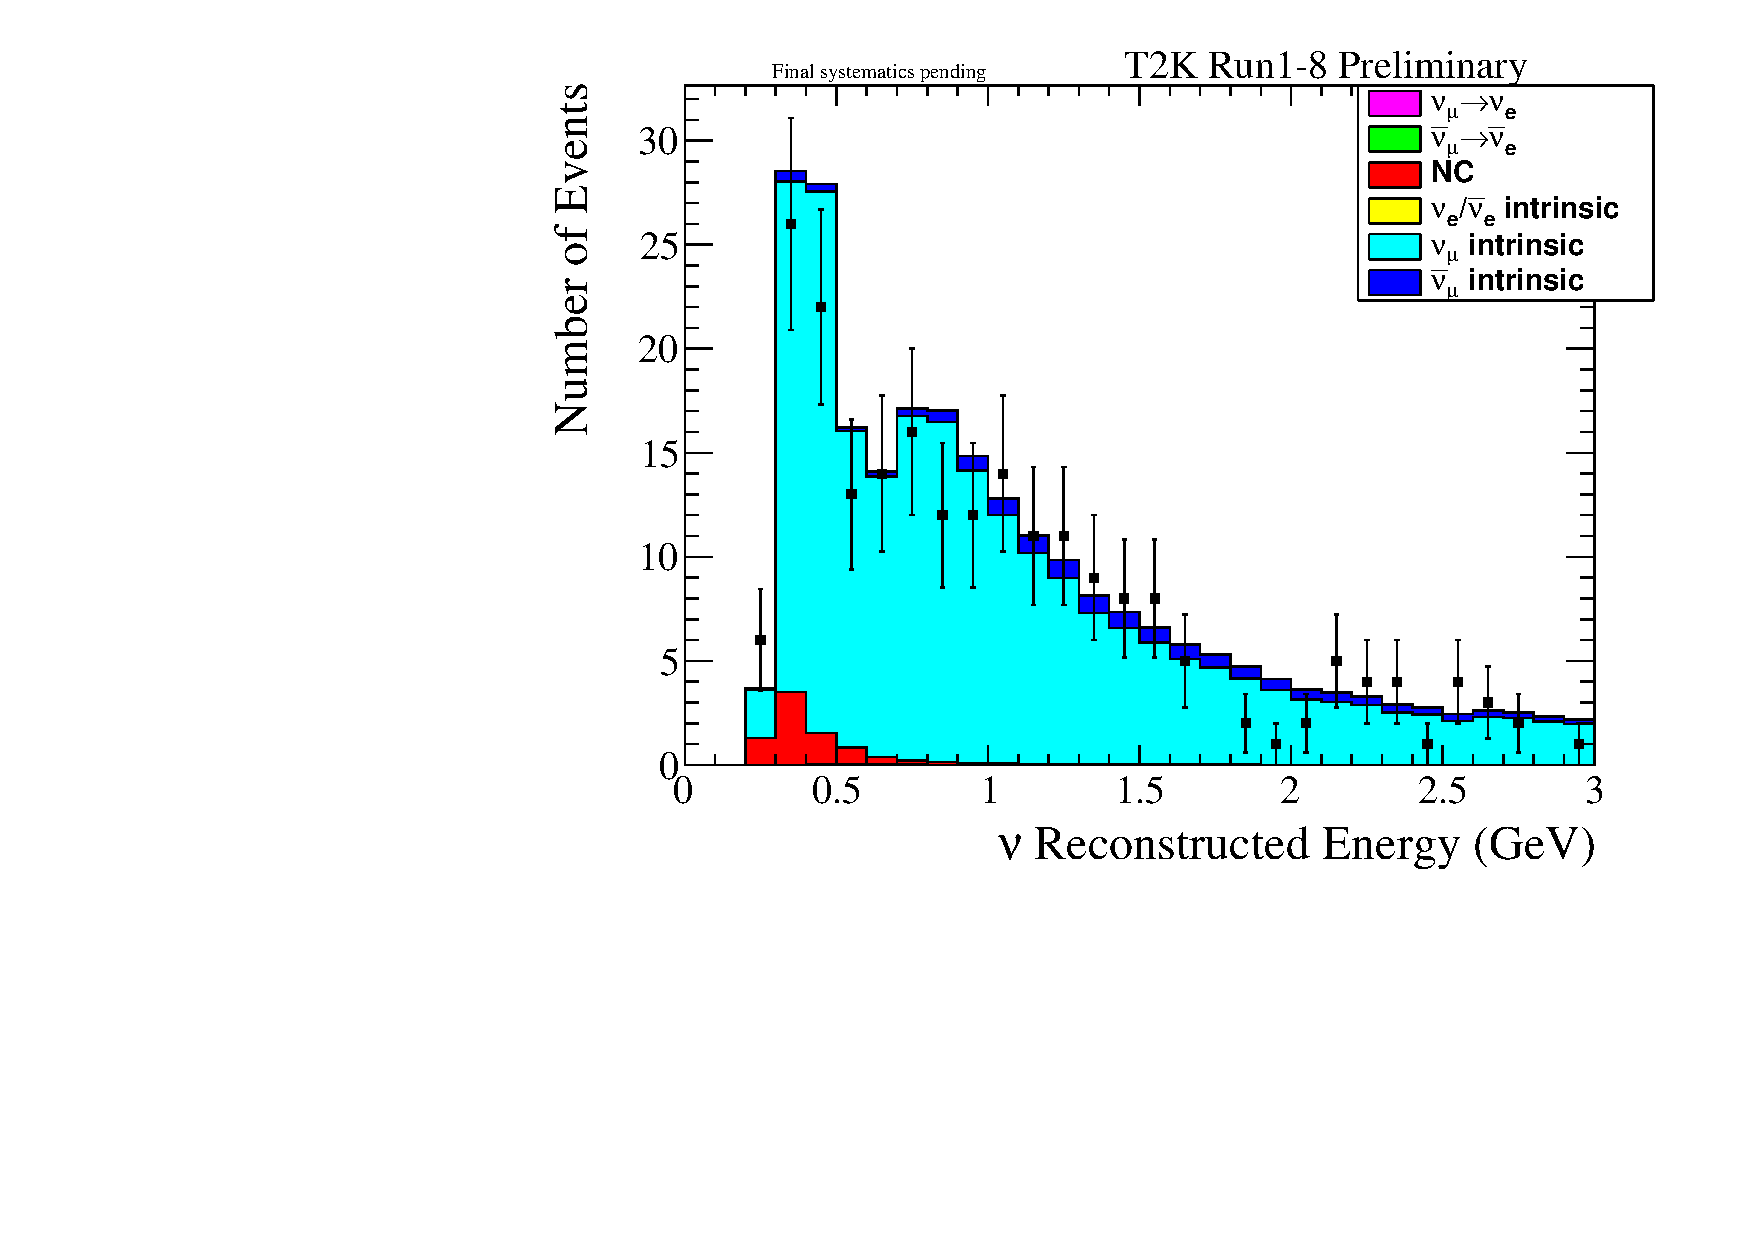
\includegraphics[width=0.9\textwidth]{spectra/spectrum_osc_asimovpf_1Rmu_data}
		\caption{Muon-like, neutrino mode}
	\end{subfigure}
	\begin{subfigure}[b]{0.49\textwidth}
		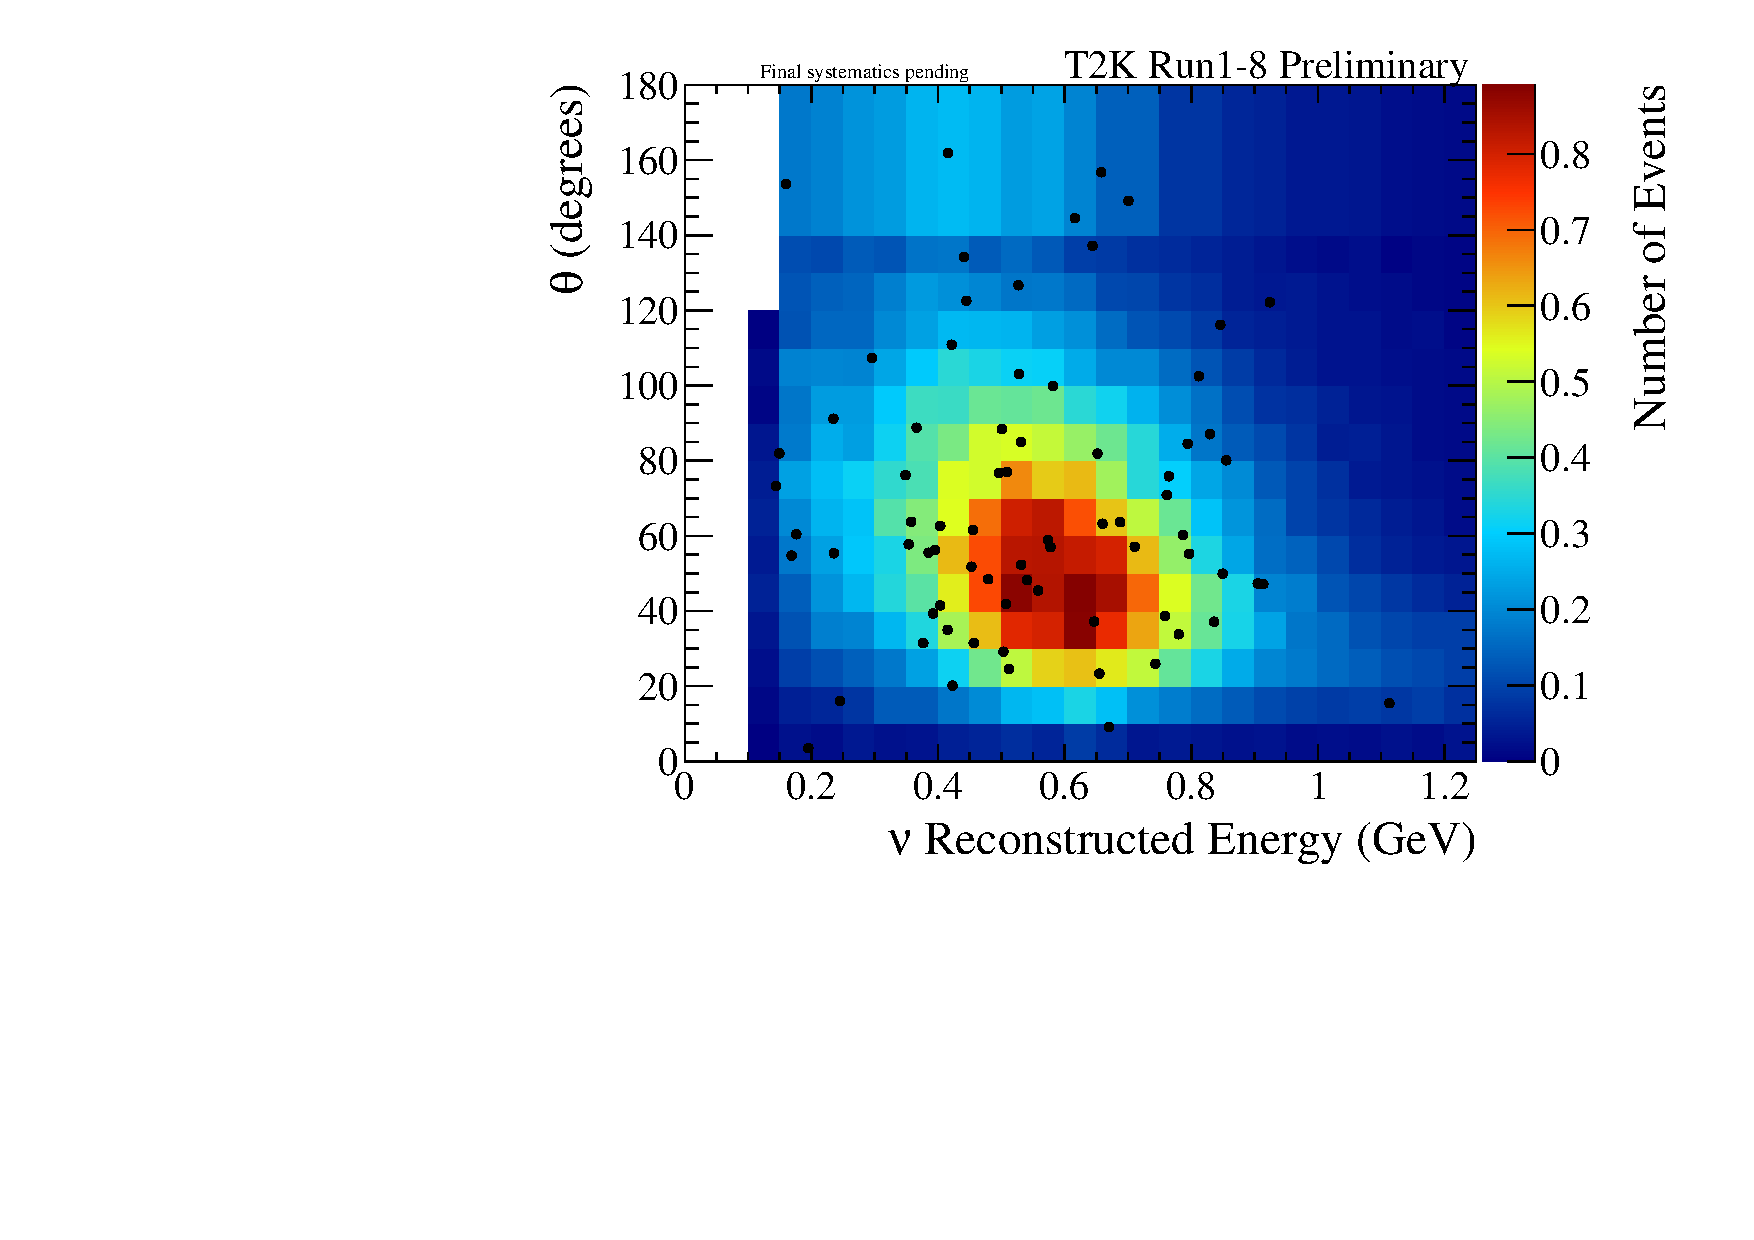
\includegraphics[width=0.9\textwidth]{spectra/spectrum_osc_asimovpf_1Re_data}
		\caption{Electron-like, neutrino mode}
	\end{subfigure}
	\begin{subfigure}[b]{0.49\textwidth}
		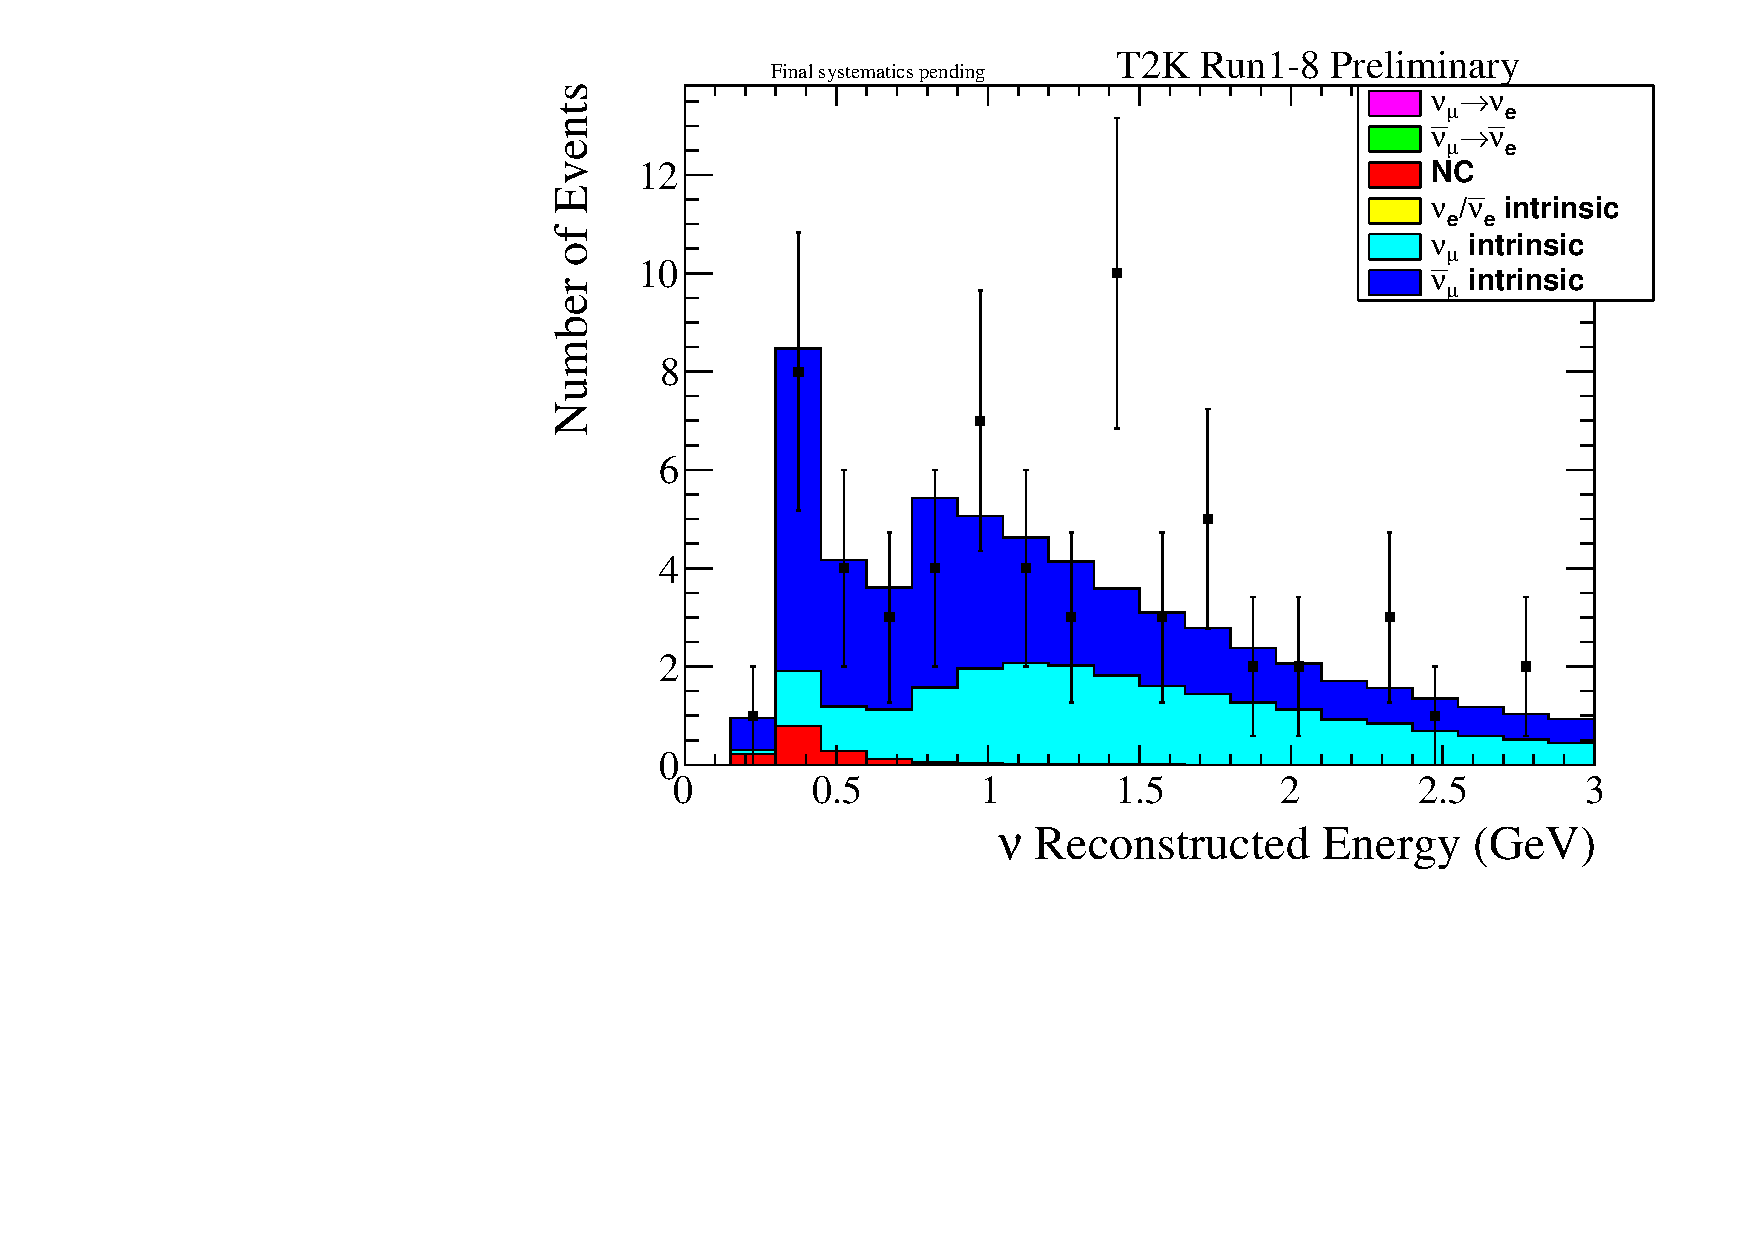
\includegraphics[width=0.9\textwidth]{spectra/spectrum_osc_asimovpf_RHC1Rmu_data}
		\caption{Muon-like, antineutrino mode}
	\end{subfigure}
	\begin{subfigure}[b]{0.49\textwidth}
		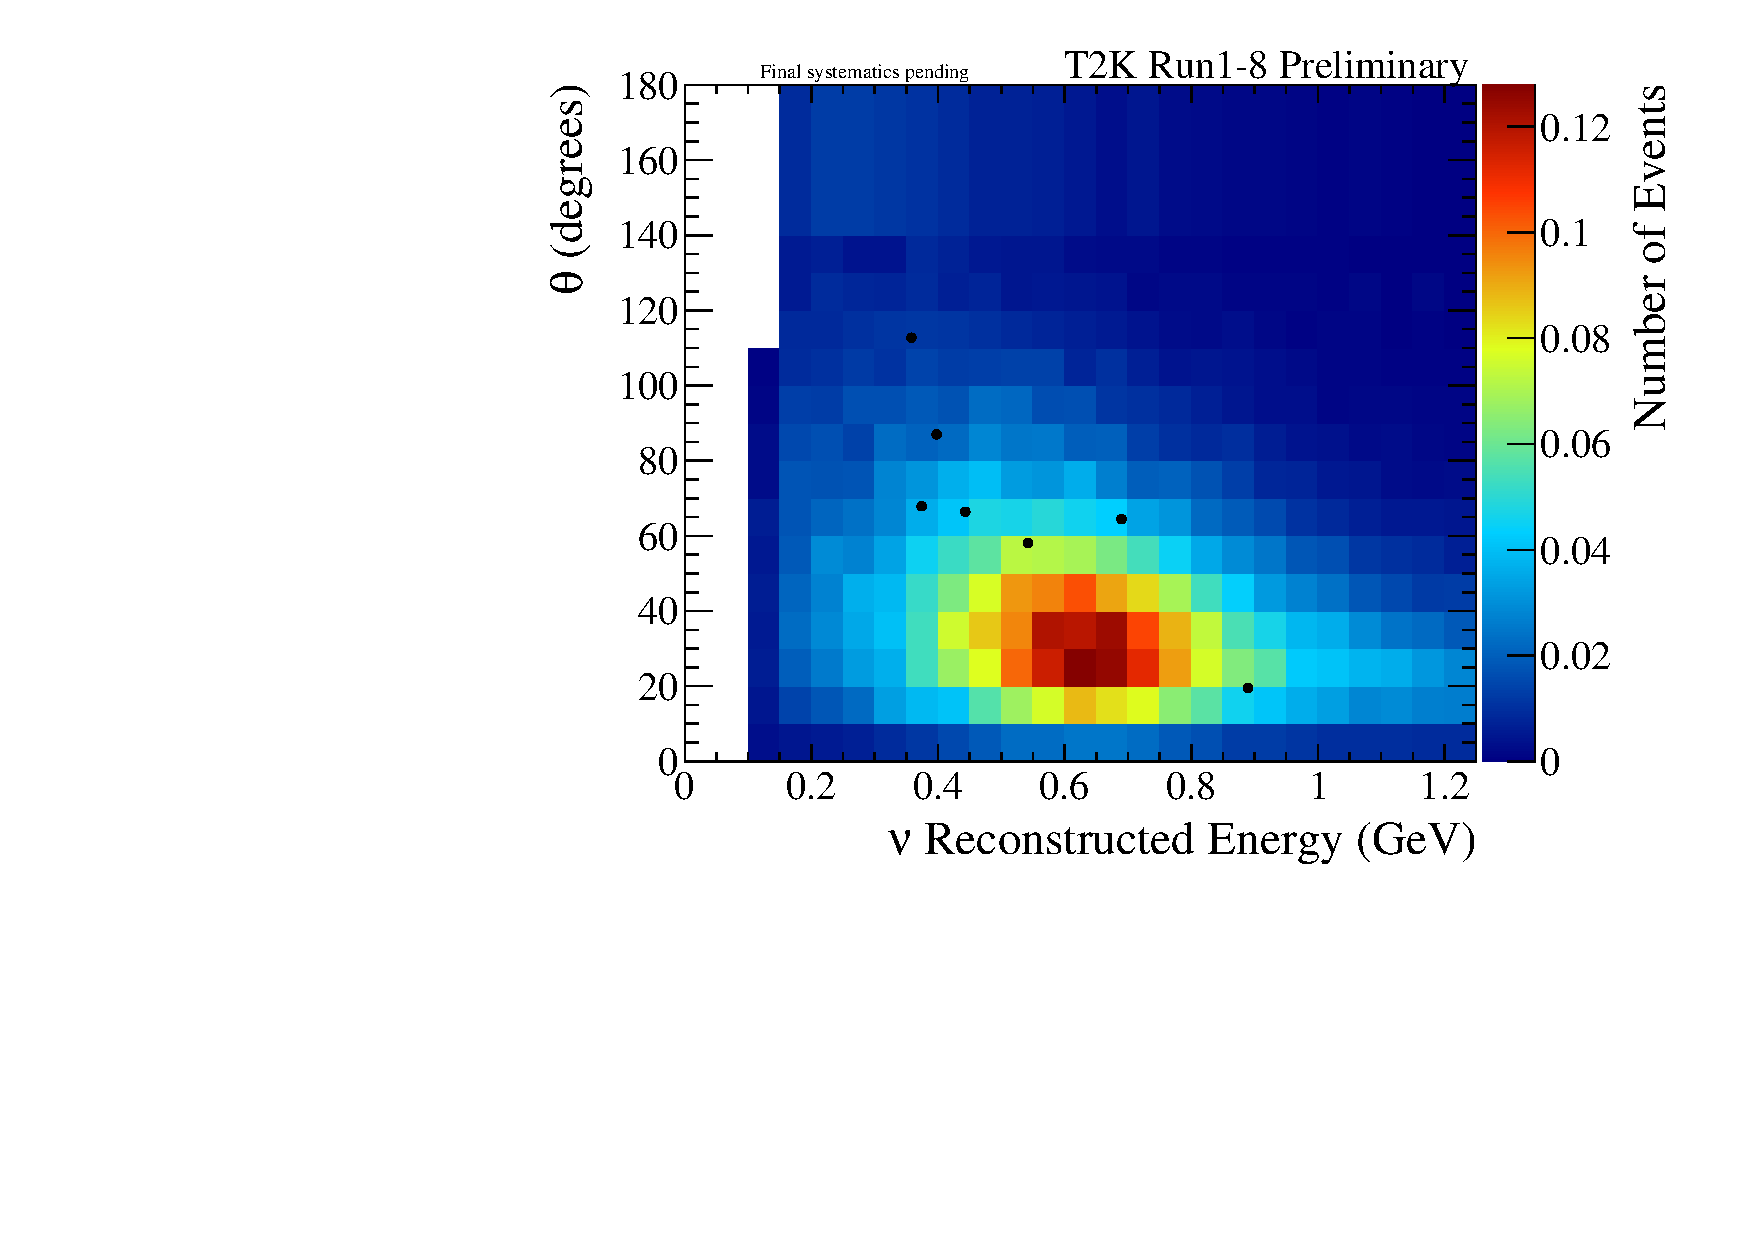
\includegraphics[width=0.9\textwidth]{spectra/spectrum_osc_asimovpf_RHC1Re_data}
		\caption{Electron-like antineutrino mode}
	\end{subfigure}
	\begin{subfigure}[b]{0.49\textwidth}
		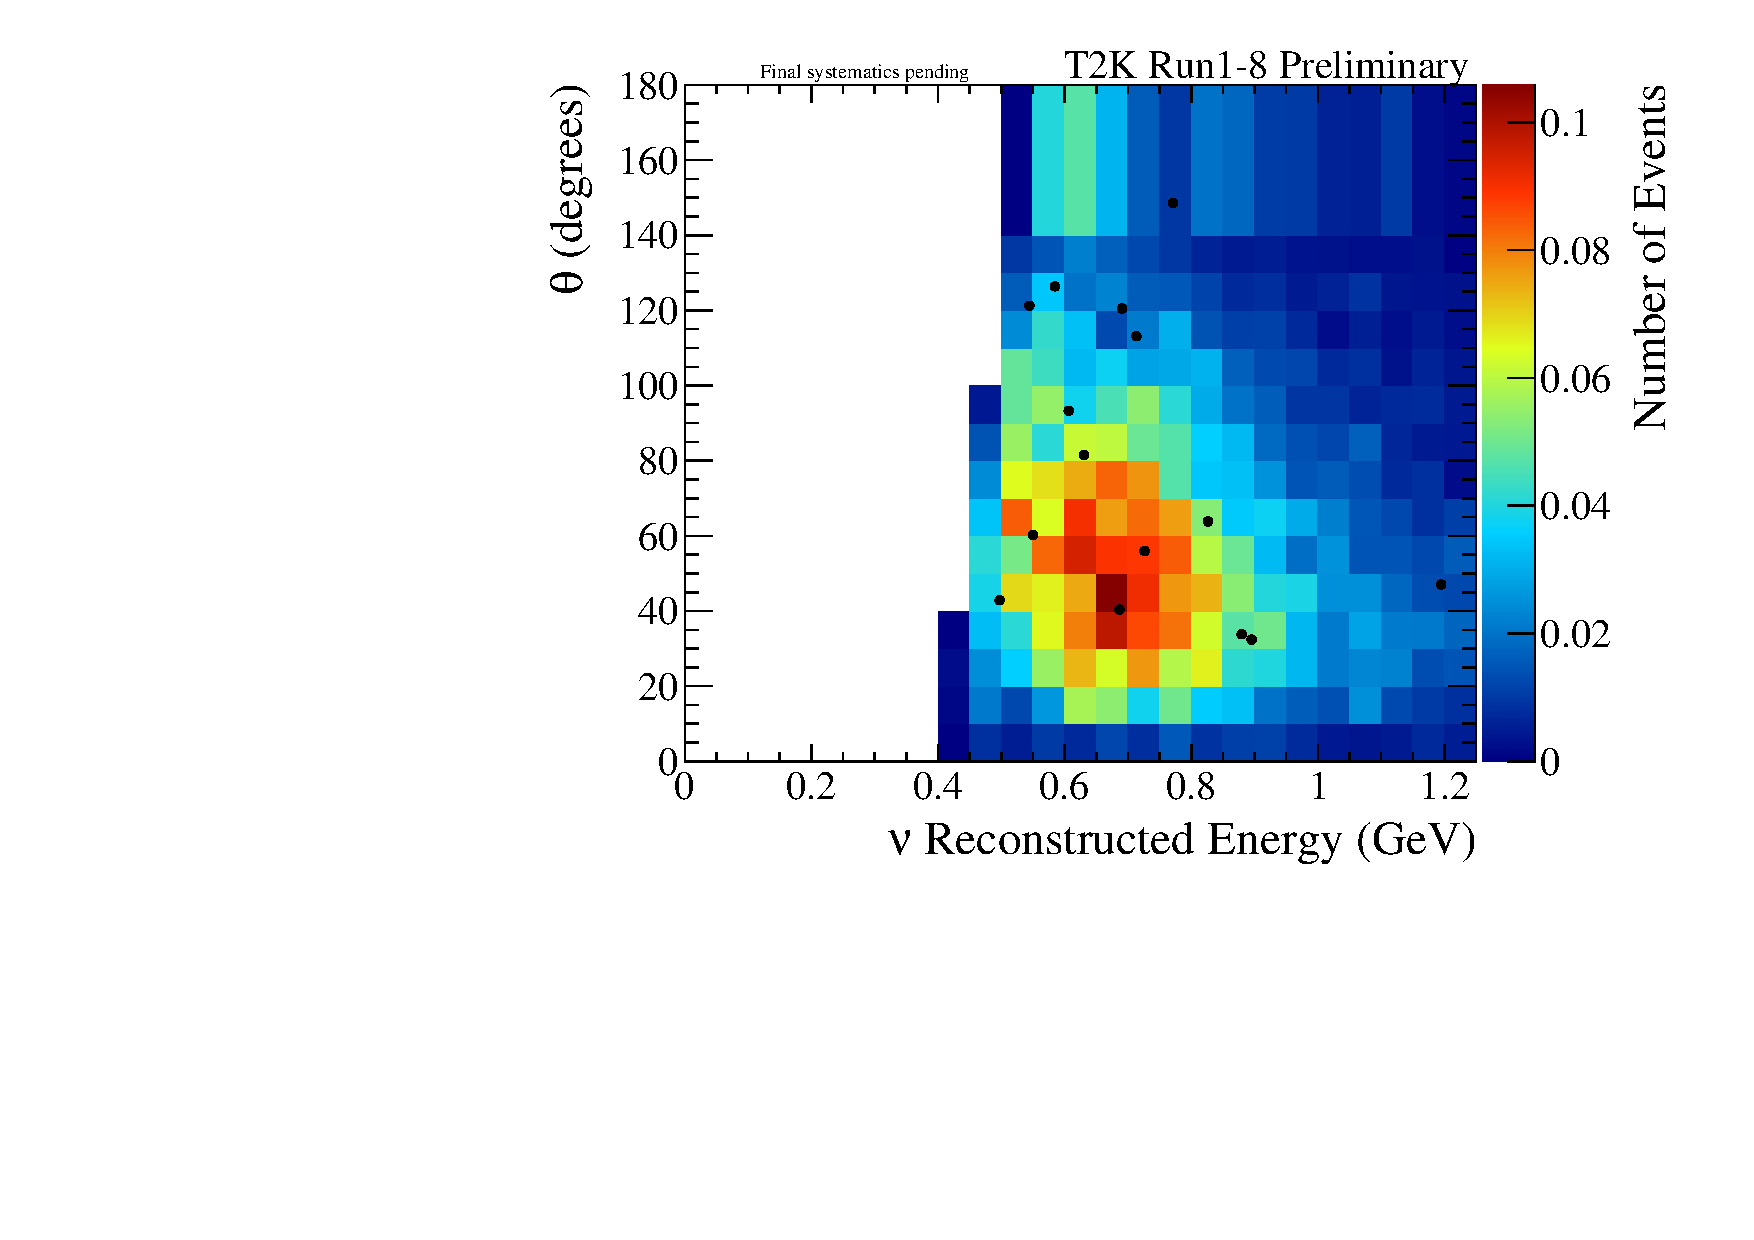
\includegraphics[width=0.9\textwidth]{spectra/spectrum_osc_asimovpf_MultiRe_data}
		\caption{\nueCConepi-like, neutrino mode}
	\end{subfigure}
	\caption {
		Predicted spectra and observed events (points). $\mu$-like distributions are a function of the reconstructed neutrino energy, while the $e$-like, including \nueCConepi, distributions are functions of both the reconstructed neutrino energy and the reconstructed angle between the outgoing lepton and the neutrino direction. The distributions correspond to the statistics collected in the full \RunPeriod data set. The spectra are generated with the systematic parameters described in \cref{sec:systematics} and the oscillation parameters corresponding to the best-fit values from the data fit (solar parameters at PDG 2016).
	}
	\label{fig:asimovpf_spectra_mc_data}
\end{figure*}
\clearpage
\begin{figure*}[htb]
	\center

	\begin{subfigure}[b]{0.49\textwidth}
		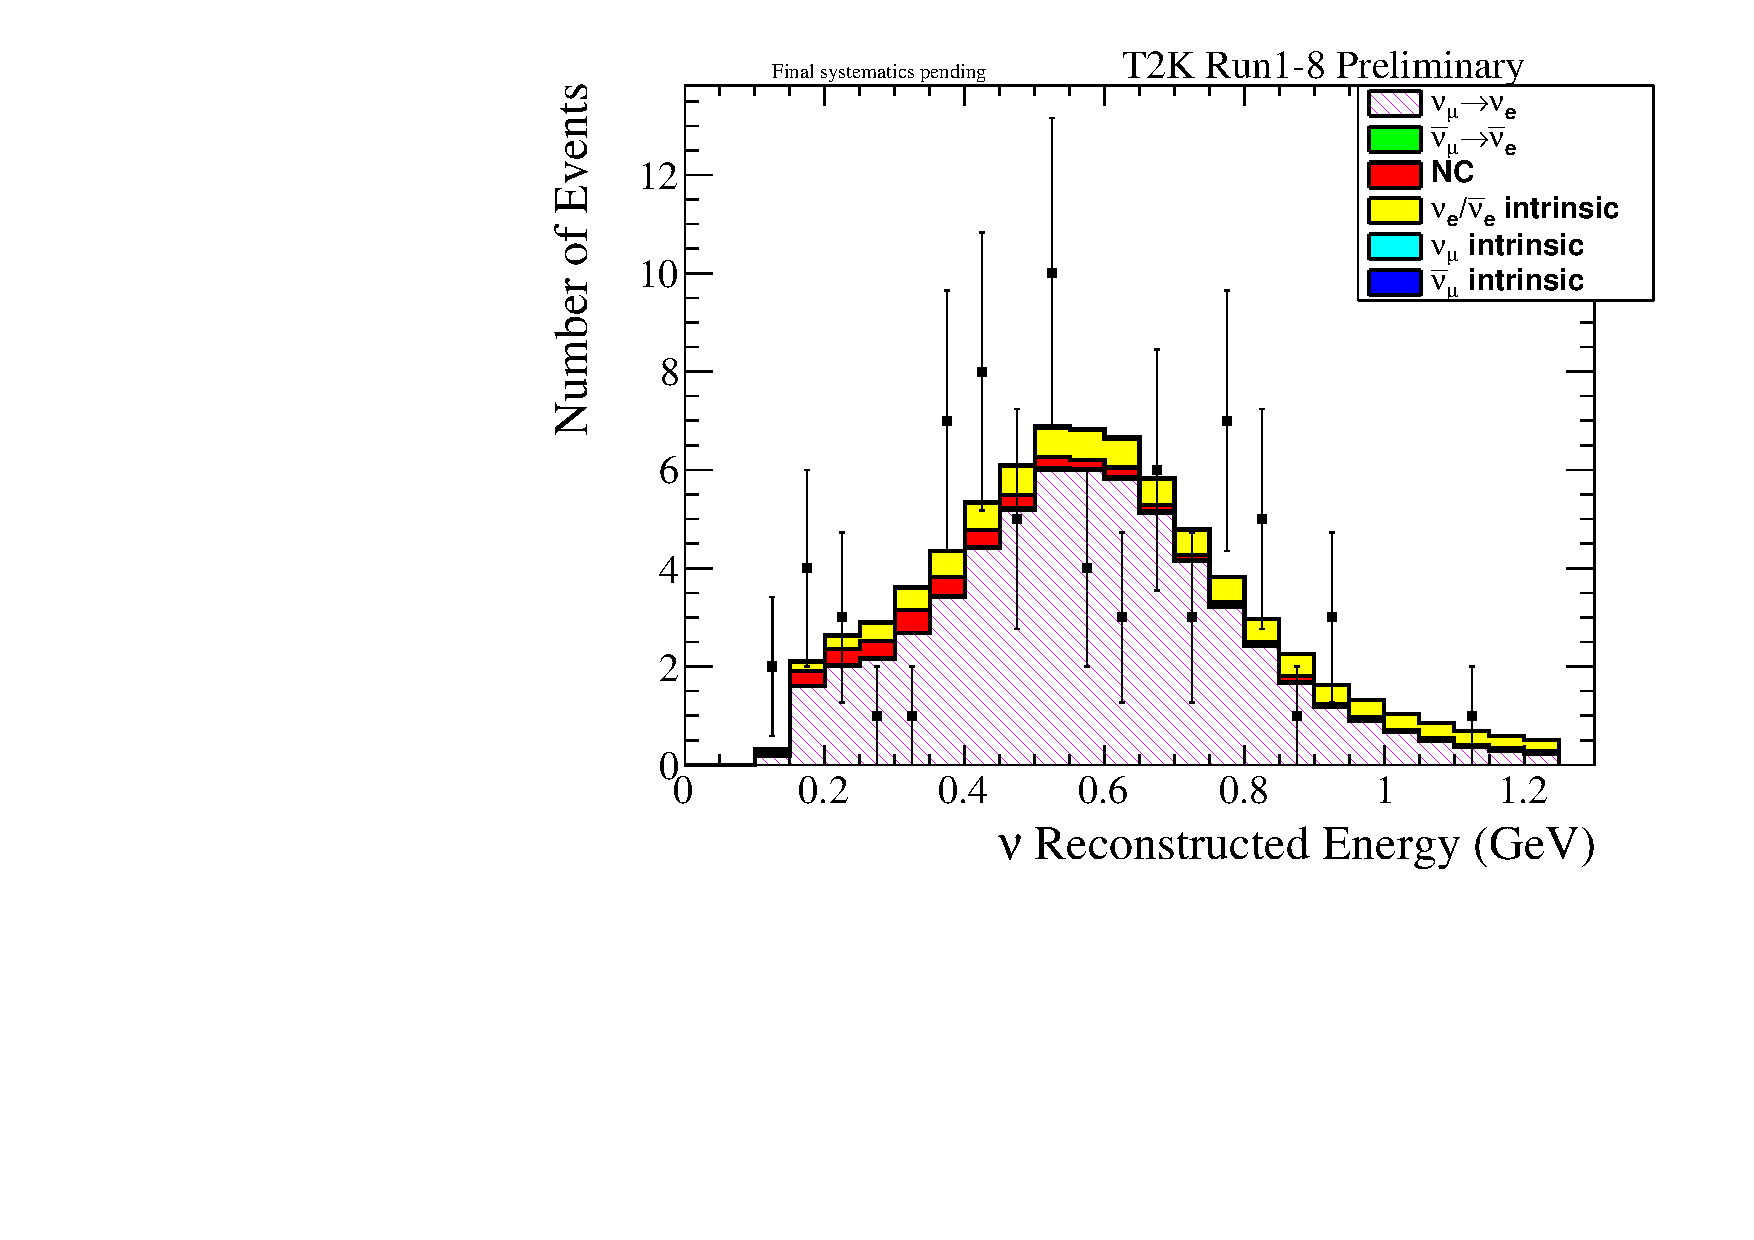
\includegraphics[width=0.9\textwidth]{spectra/erec_spectrum_osc_asimovpf_1Re_data}
		\caption{Electron-like, neutrino mode}
	\end{subfigure}
	\begin{subfigure}[b]{0.49\textwidth}
		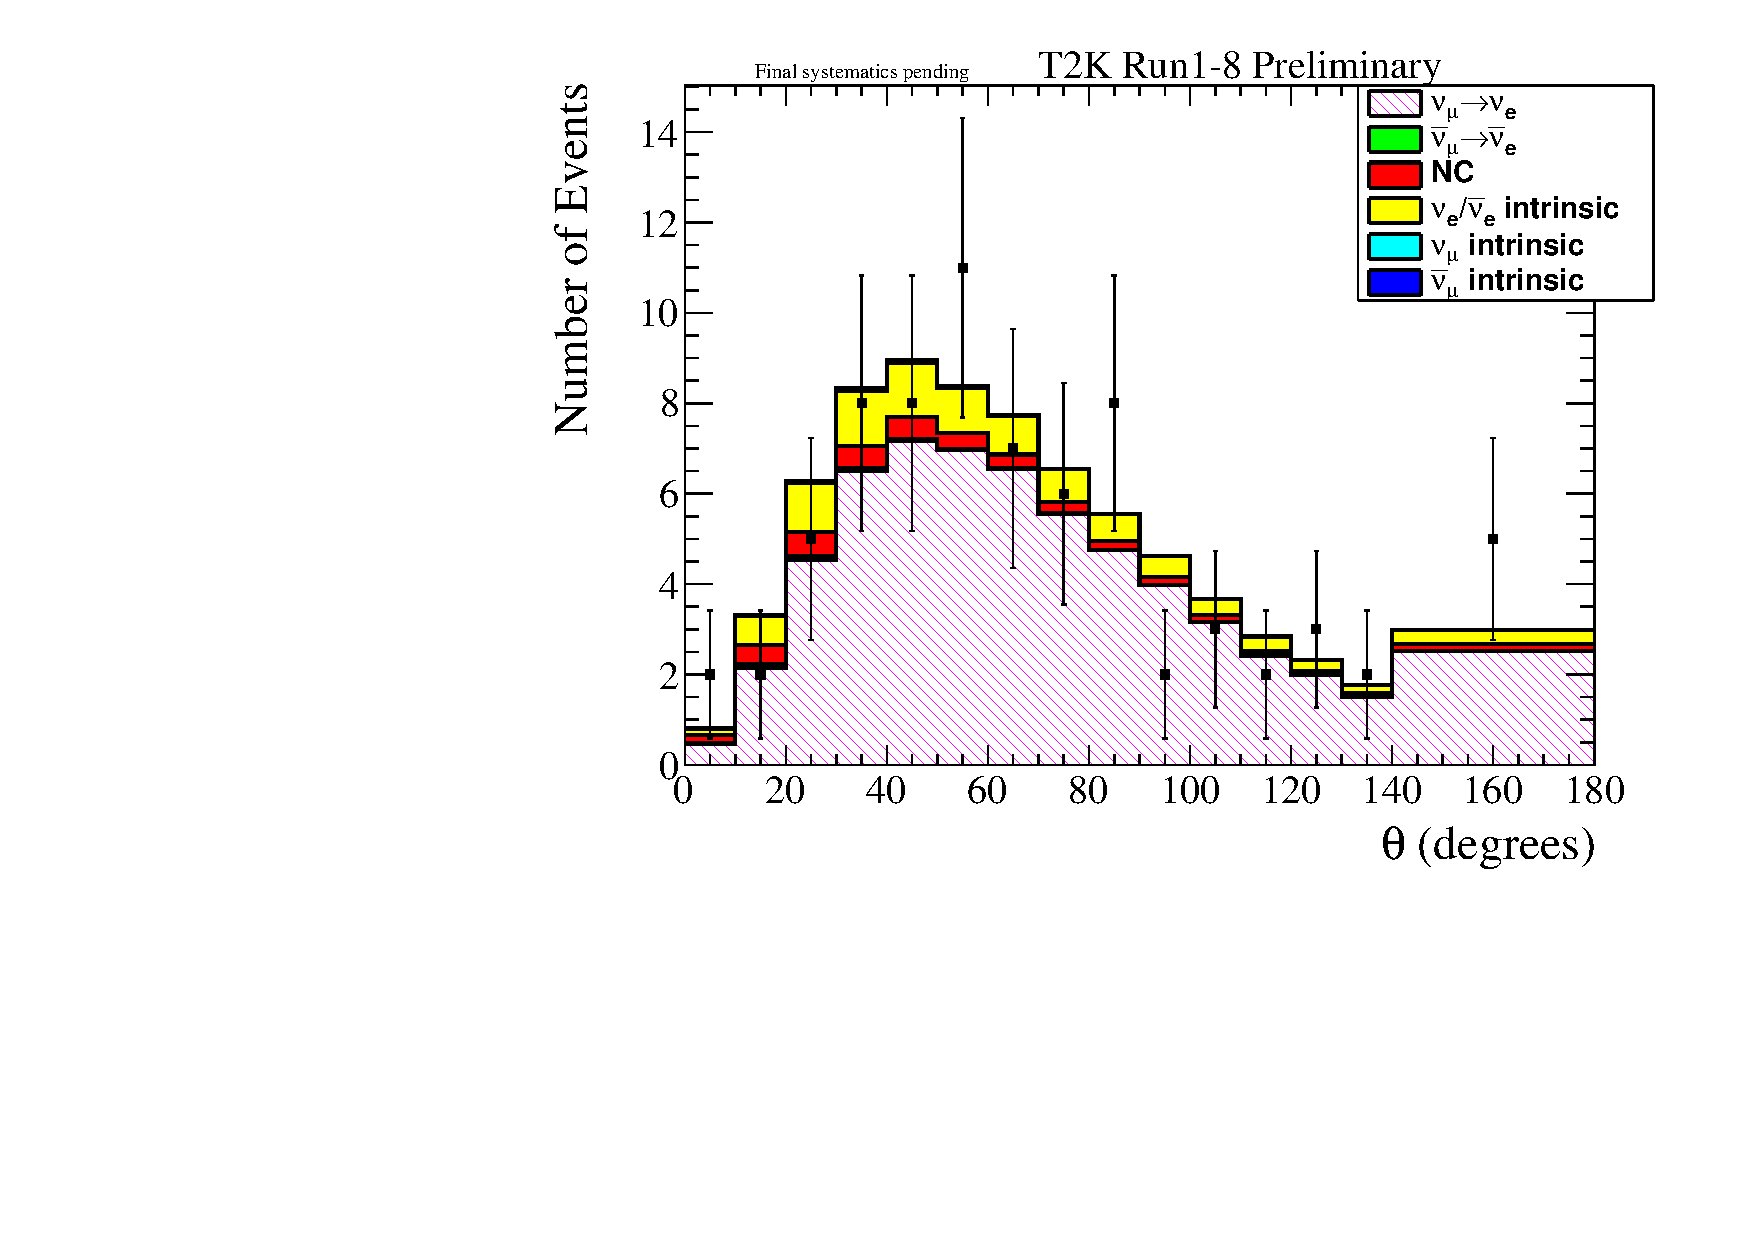
\includegraphics[width=0.9\textwidth]{spectra/theta_spectrum_osc_asimovpf_1Re_data}
		\caption{Electron-like, neutrino mode}
	\end{subfigure}

	\begin{subfigure}[b]{0.49\textwidth}
		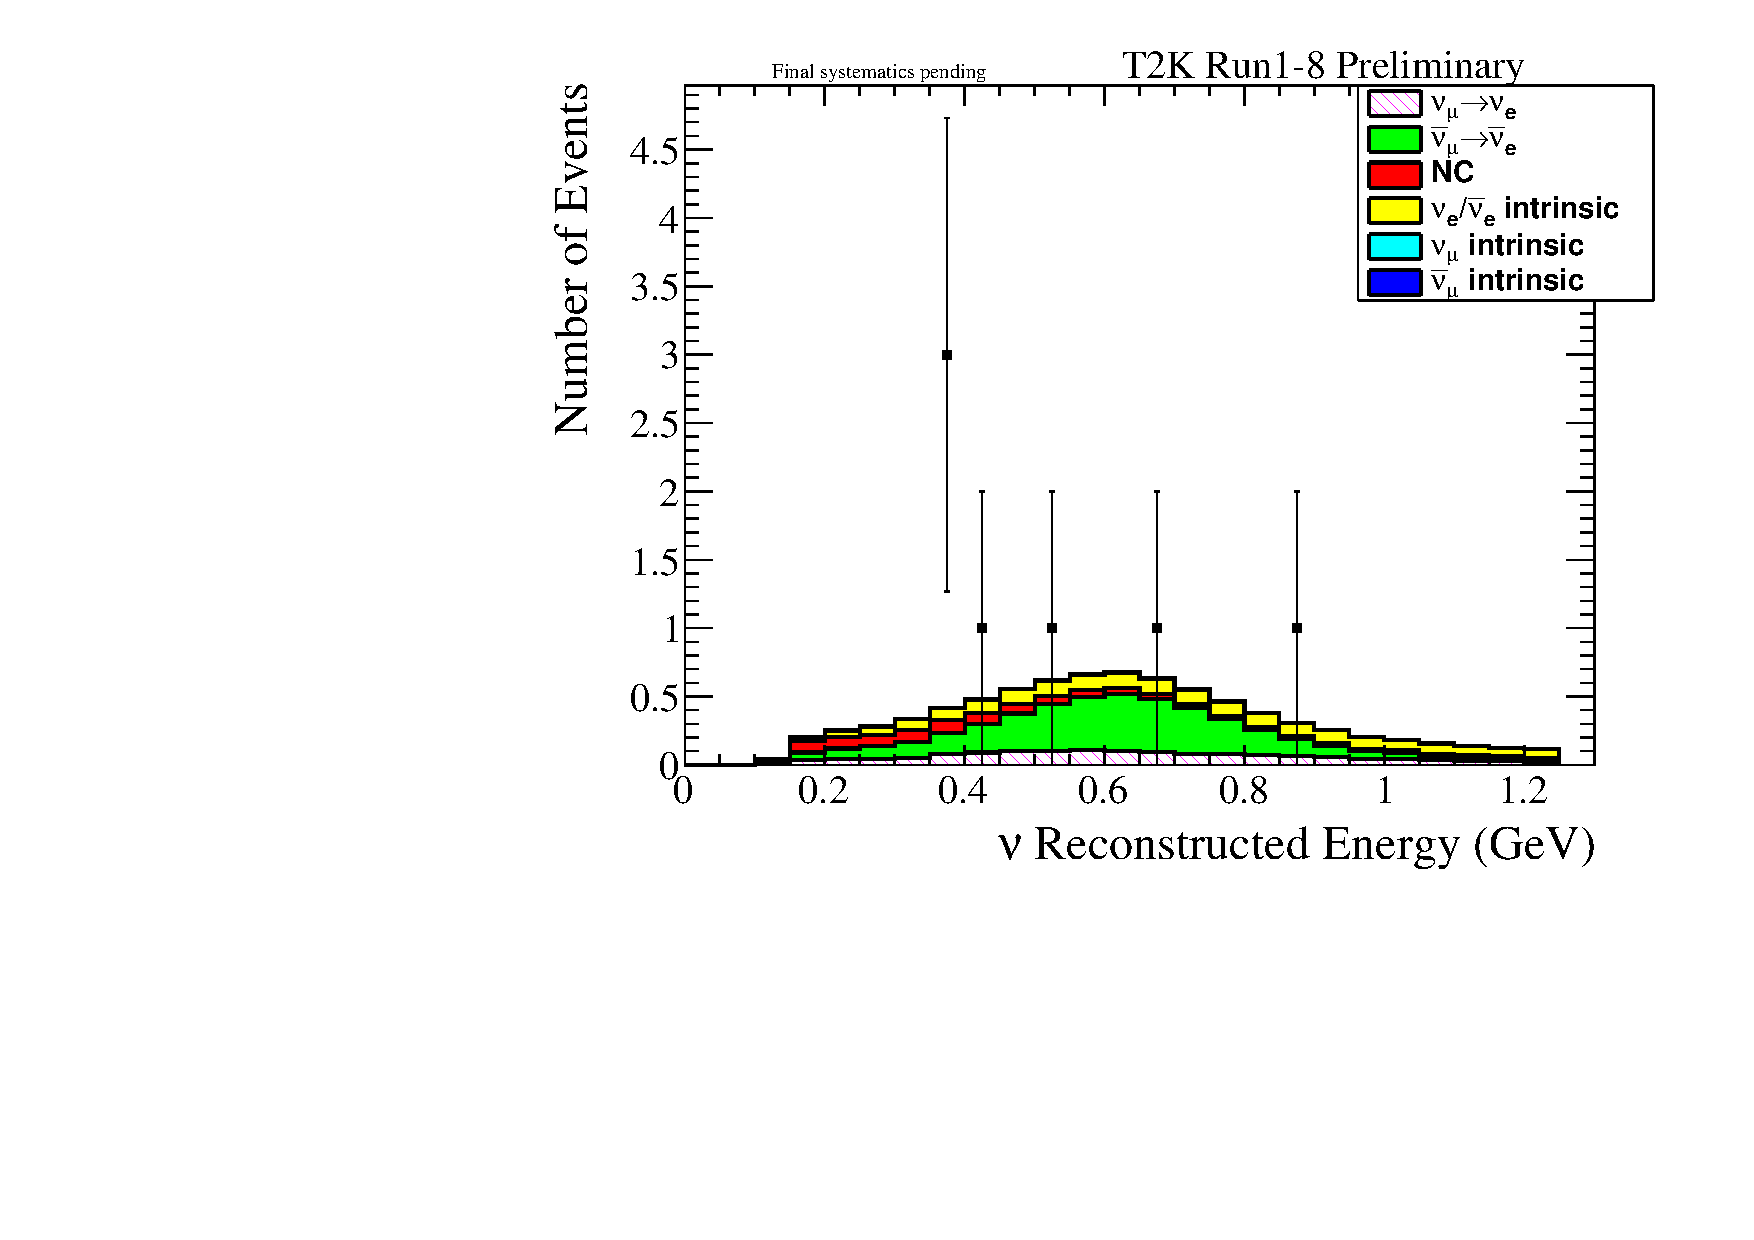
\includegraphics[width=0.9\textwidth]{spectra/erec_spectrum_osc_asimovpf_RHC1Re_data}
		\caption{Electron-like antineutrino mode}
	\end{subfigure}
	\begin{subfigure}[b]{0.49\textwidth}
		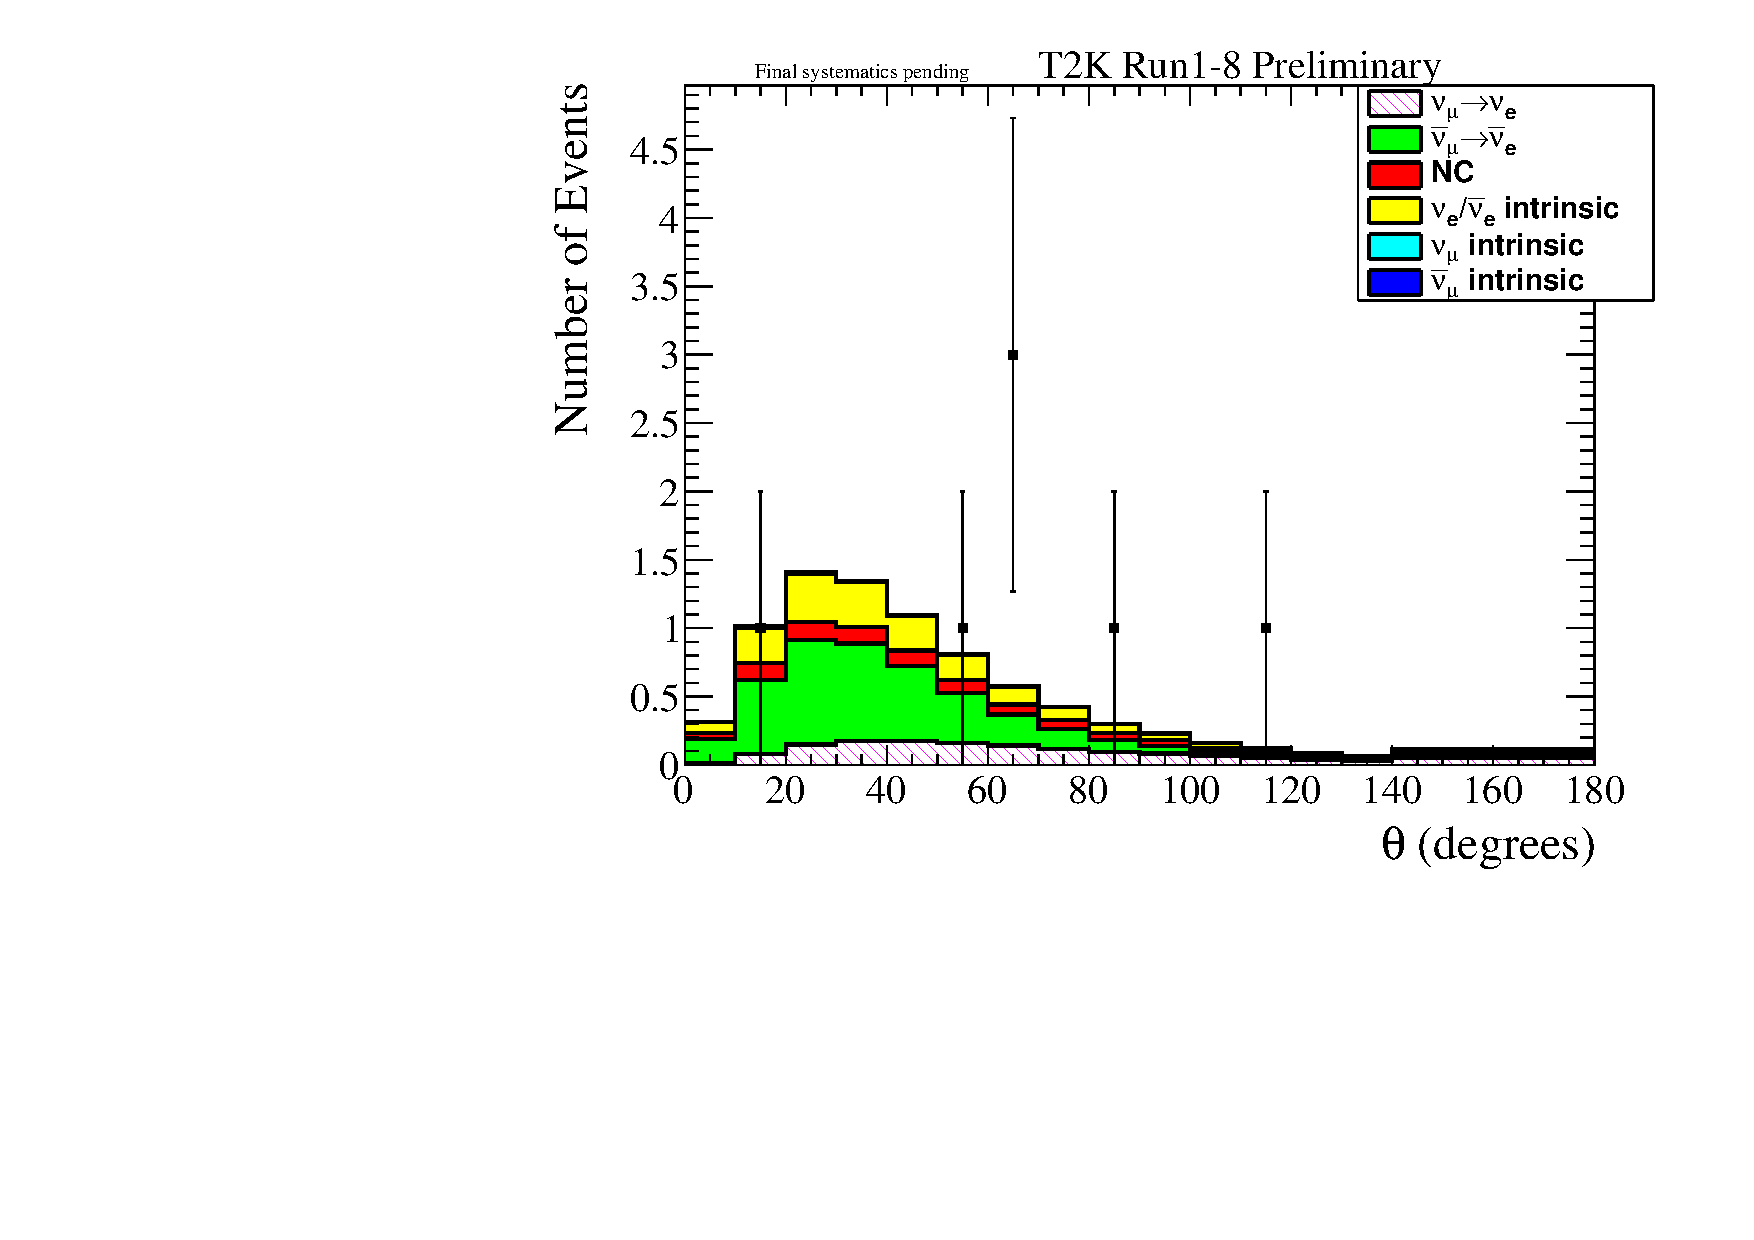
\includegraphics[width=0.9\textwidth]{spectra/theta_spectrum_osc_asimovpf_RHC1Re_data}
		\caption{Electron-like antineutrino mode}
	\end{subfigure}

	\begin{subfigure}[b]{0.49\textwidth}
		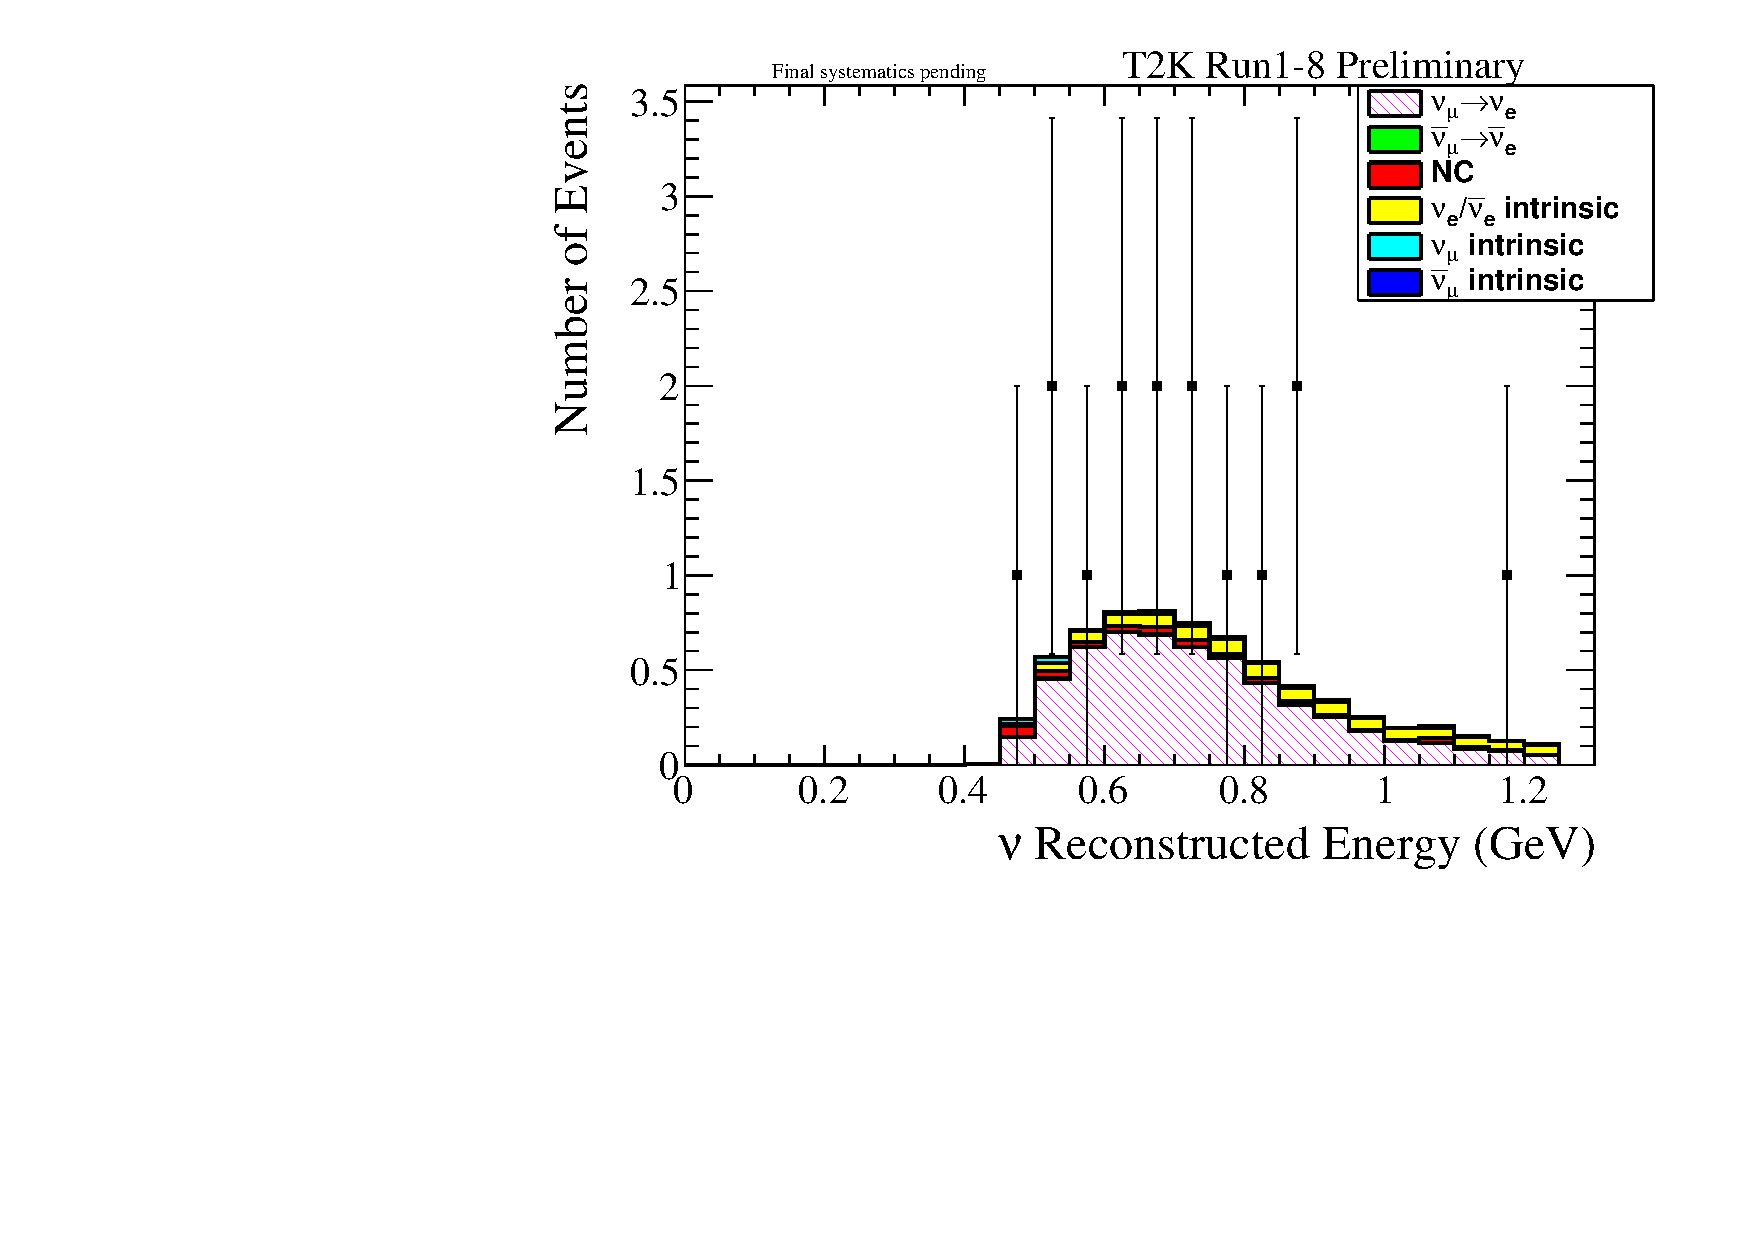
\includegraphics[width=0.9\textwidth]{spectra/erec_spectrum_osc_asimovpf_MultiRe_data}
		\caption{\nueCConepi-like, neutrino mode}
	\end{subfigure}
	\begin{subfigure}[b]{0.49\textwidth}
		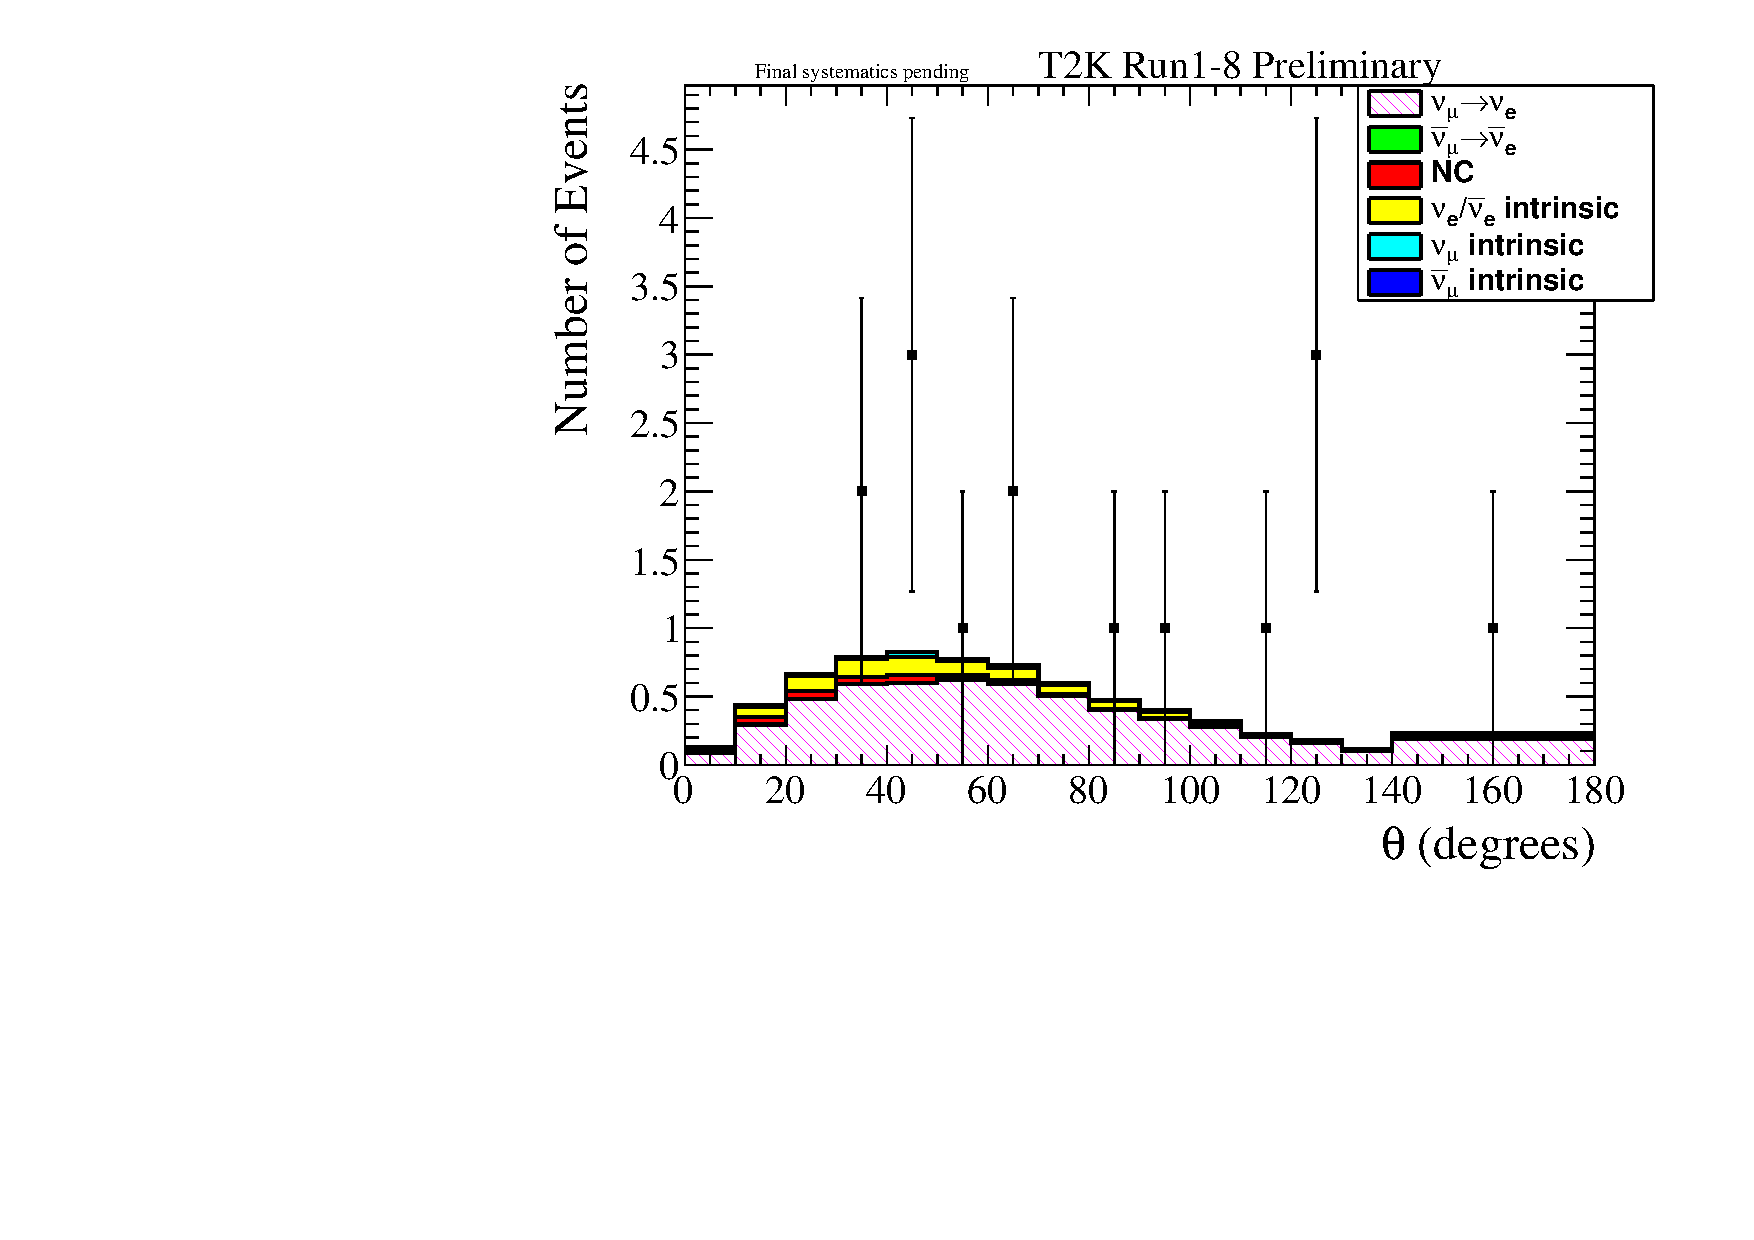
\includegraphics[width=0.9\textwidth]{spectra/theta_spectrum_osc_asimovpf_MultiRe_data}
		\caption{\nueCConepi-like, neutrino mode}
	\end{subfigure}
	\caption {
		Predicted spectra and observed events (points). The $e$-like, including \nueCConepi, distributions are functions of both the reconstructed neutrino energy and the reconstructed angle between the outgoing lepton and the neutrino direction, with the projections in each variable shown here. The distributions correspond to the statistics collected in the full \RunPeriod data set. The spectra are generated with the systematic parameters described in \cref{sec:systematics} and the oscillation parameters corresponding to the best-fit values from the data fit (solar parameters at PDG 2016).
	}
	\label{fig:asimovpf_spectra_mc_data_elike_1D}
\end{figure*}
\clearpage

The best-fit values and $1\sigma$ ranges for each oscillation parameter are shown in \cref{tab:data_bestfit} for normal hierarchy (which is preferred in all data fits). The $1\sigma$ ranges are extracted for each oscillation parameter from the 1-dimensional $\Delta \chi^2$ distributions shown in \crefrange{fig:dcp_data}{fig:dmsq23_data}.

The 1-dimensional contours are plotted with respect to the global minimum from normal and inverted hierarchies, while the 2-dimensional confidence intervals are shown drawing the normal and inverted hierarchy contours independently, i.e. each contour is produced with respect to the global minimum under that hierarchy hypothesis.

%The reactor measurements are in agreement with the T2K data at $1\sigma$ level if $\delta_{CP} \sim - \frac{\pi}{2}$. Furthermore we can see that the region close $\delta_{CP} = + \pi/2$ is excluded at 90\% CL.

\begin{table}
\centering
\begin{tabular}{| c | c | c | c | c | c |}
\hline
Parameter & Reactor & Best-fit (NH) & $\pm1\sigma$ (NH) & Best-fit (IH) & $\pm1\sigma$ (IH) \\
\hline
\deltacp & Yes & \BestFitDeltacpwRC & [\MOneSigmaDeltacpwRC,\POneSigmaDeltacpwRC] & \BestFitDeltacpwRCIH & [\MOneSigmaDeltacpwRCIH,\POneSigmaDeltacpwRCIH] \\
\deltacp & No & \BestFitDeltacpwoRC & [\MOneSigmaDeltacpwoRC,\POneSigmaDeltacpwoRC] & \BestFitDeltacpwoRCIH & [\MOneSigmaDeltacpwoRCIH,\POneSigmaDeltacpwoRCIH] \\
\ssqthonethree & No & \BestFitMixingOneThreewoRC & [\MOneMixingOneThreewoRC,\POneMixingOneThreewoRC] & \BestFitMixingOneThreewoRCIH & [\MOneMixingOneThreewoRCIH,\POneMixingOneThreewoRCIH] \\
\ssqthtwothree & Yes & \BestFitMixingTwoThreewRC & [\MOneMixingTwoThreewRC,\POneMixingTwoThreewRC] & \BestFitMixingTwoThreewRCIH & [\MOneMixingTwoThreewRCIH,\POneMixingTwoThreewRCIH] \\
\dmsqtwothree or \dmsqonethree & Yes & \BestFitDmTwoThreewRC & [\MOneDmTwoThreewRC,\POneDmTwoThreewRC] & \BestFitDmTwoThreewRCIH & [\MOneDmTwoThreewRCIH,\POneDmTwoThreewRCIH] \\
 ($10^{-3}\text{ eV}^2\text{/c}^4$) & & & & & \\
\hline
\end{tabular}

\caption{
The \RunPeriod measured oscillation parameter best-fit and the $\pm 1\sigma$ intervals are shown for normal and inverted hierarchies with respect to the hierarchy best-fit. The $\pm 1\sigma$ interval is obtained by using the constant $\Delta \chi^2$ method. For each parameter normal hierarchy is the global best-fit.
}
\label{tab:data_bestfit}
\end{table}

\clearpage

\subsection{Results for \appearance}
In \cref{fig:ssqth13_vs_dcp_data} the result for \appearance with reactor constraint and T2K only is shown.

\begin{figure*}[htb]
	\center
	\begin{subfigure}[b]{0.49\textwidth}
		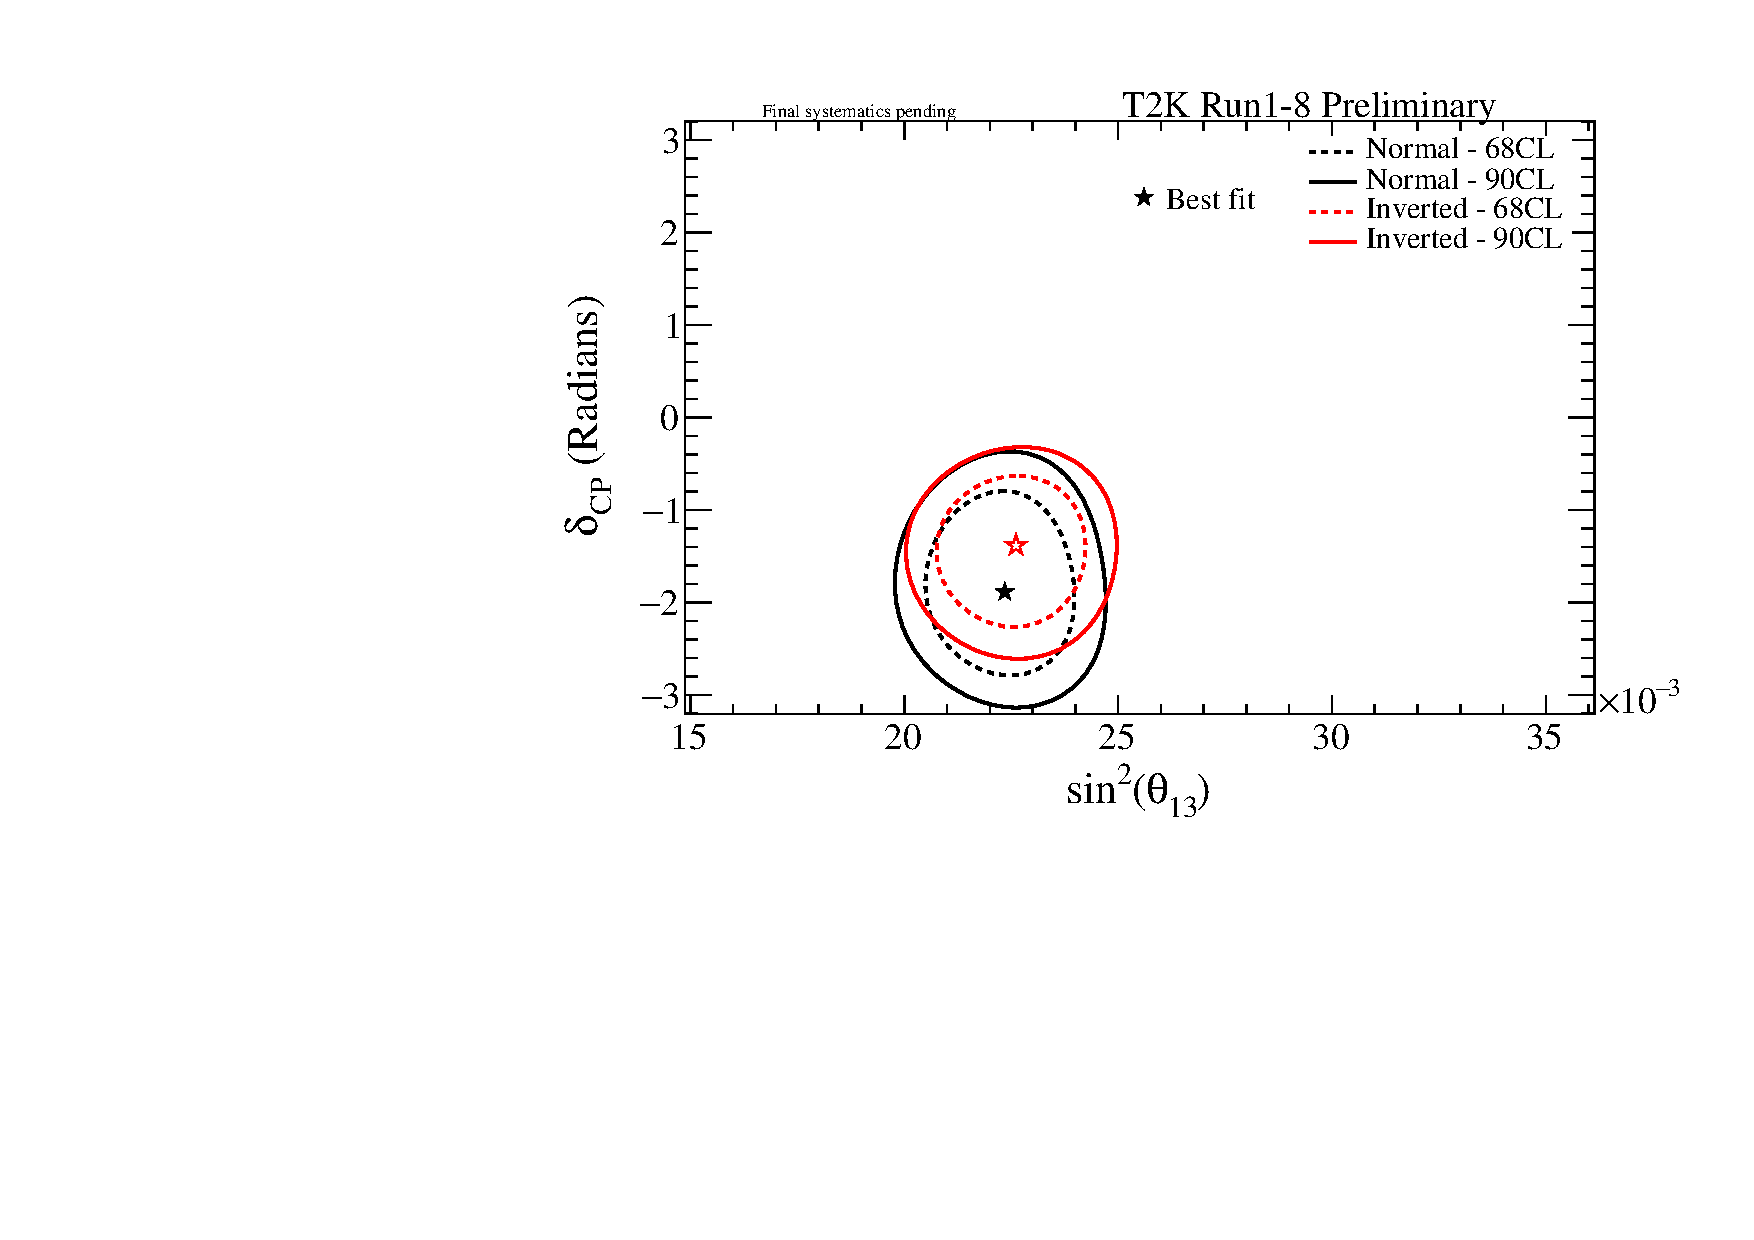
\includegraphics[width=0.9\textwidth]{data/reactor/mixing13_deltacp_data_reactor_global}
		\caption{\appearance with reactor constraint}
	\end{subfigure}
	\begin{subfigure}[b]{0.49\textwidth}
		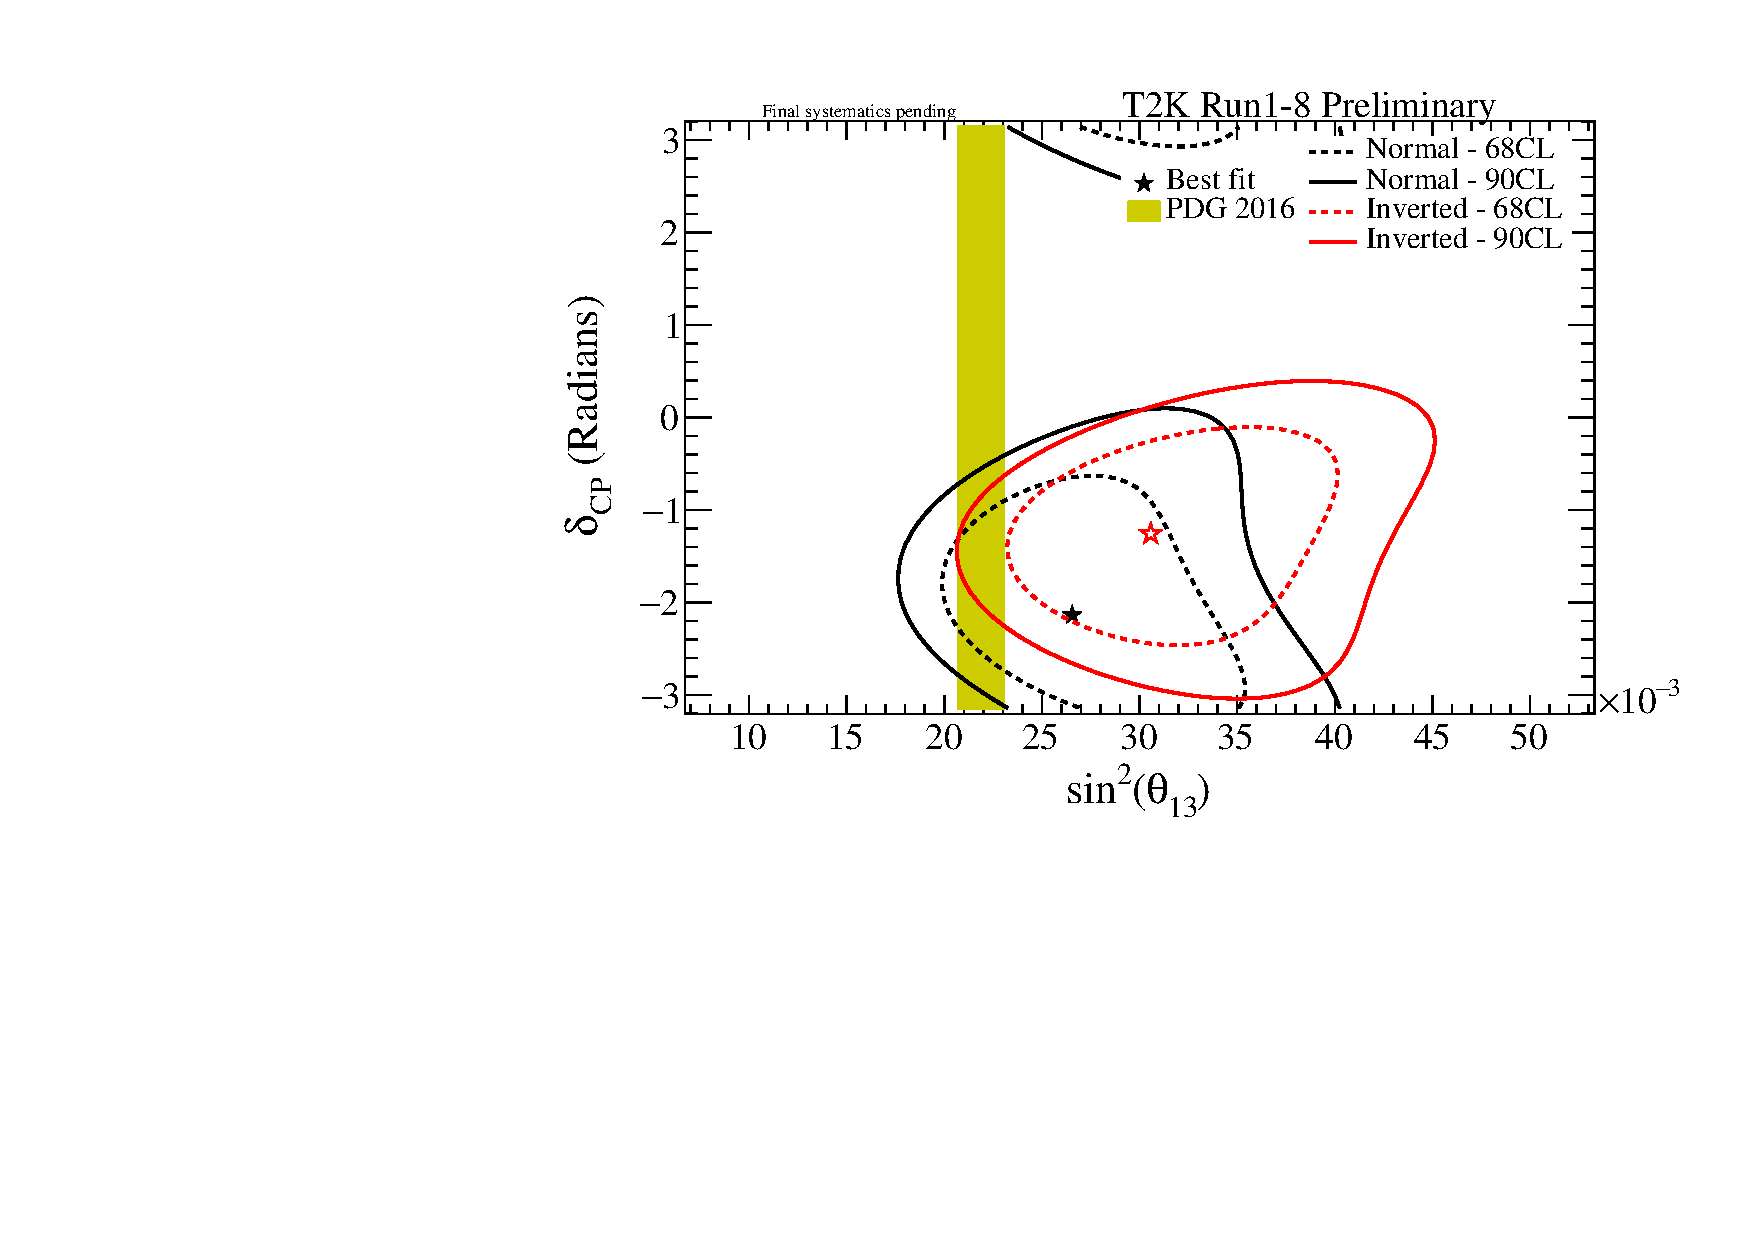
\includegraphics[width=0.9\textwidth]{data/t2k/mixing13_deltacp_data_t2k_global}
		\caption{\appearance T2K only}
	\end{subfigure}
	\caption {
		Contours at 68\% and 90\% CL for \appearance with and without reactor constraint. Normal and inverted hierarchy contours are independent. All 5 samples were used to produce these fits.
	}
	\label{fig:ssqth13_vs_dcp_data}
\end{figure*}

\subsection{Results for \disappearance}

The result for \disappearance with reactor constraint and T2K only is shown in fig.~\ref{fig:ssqth23_vs_dmsq23_data}.

\begin{figure*}[htb]
	\center
	\begin{subfigure}[b]{0.49\textwidth}
		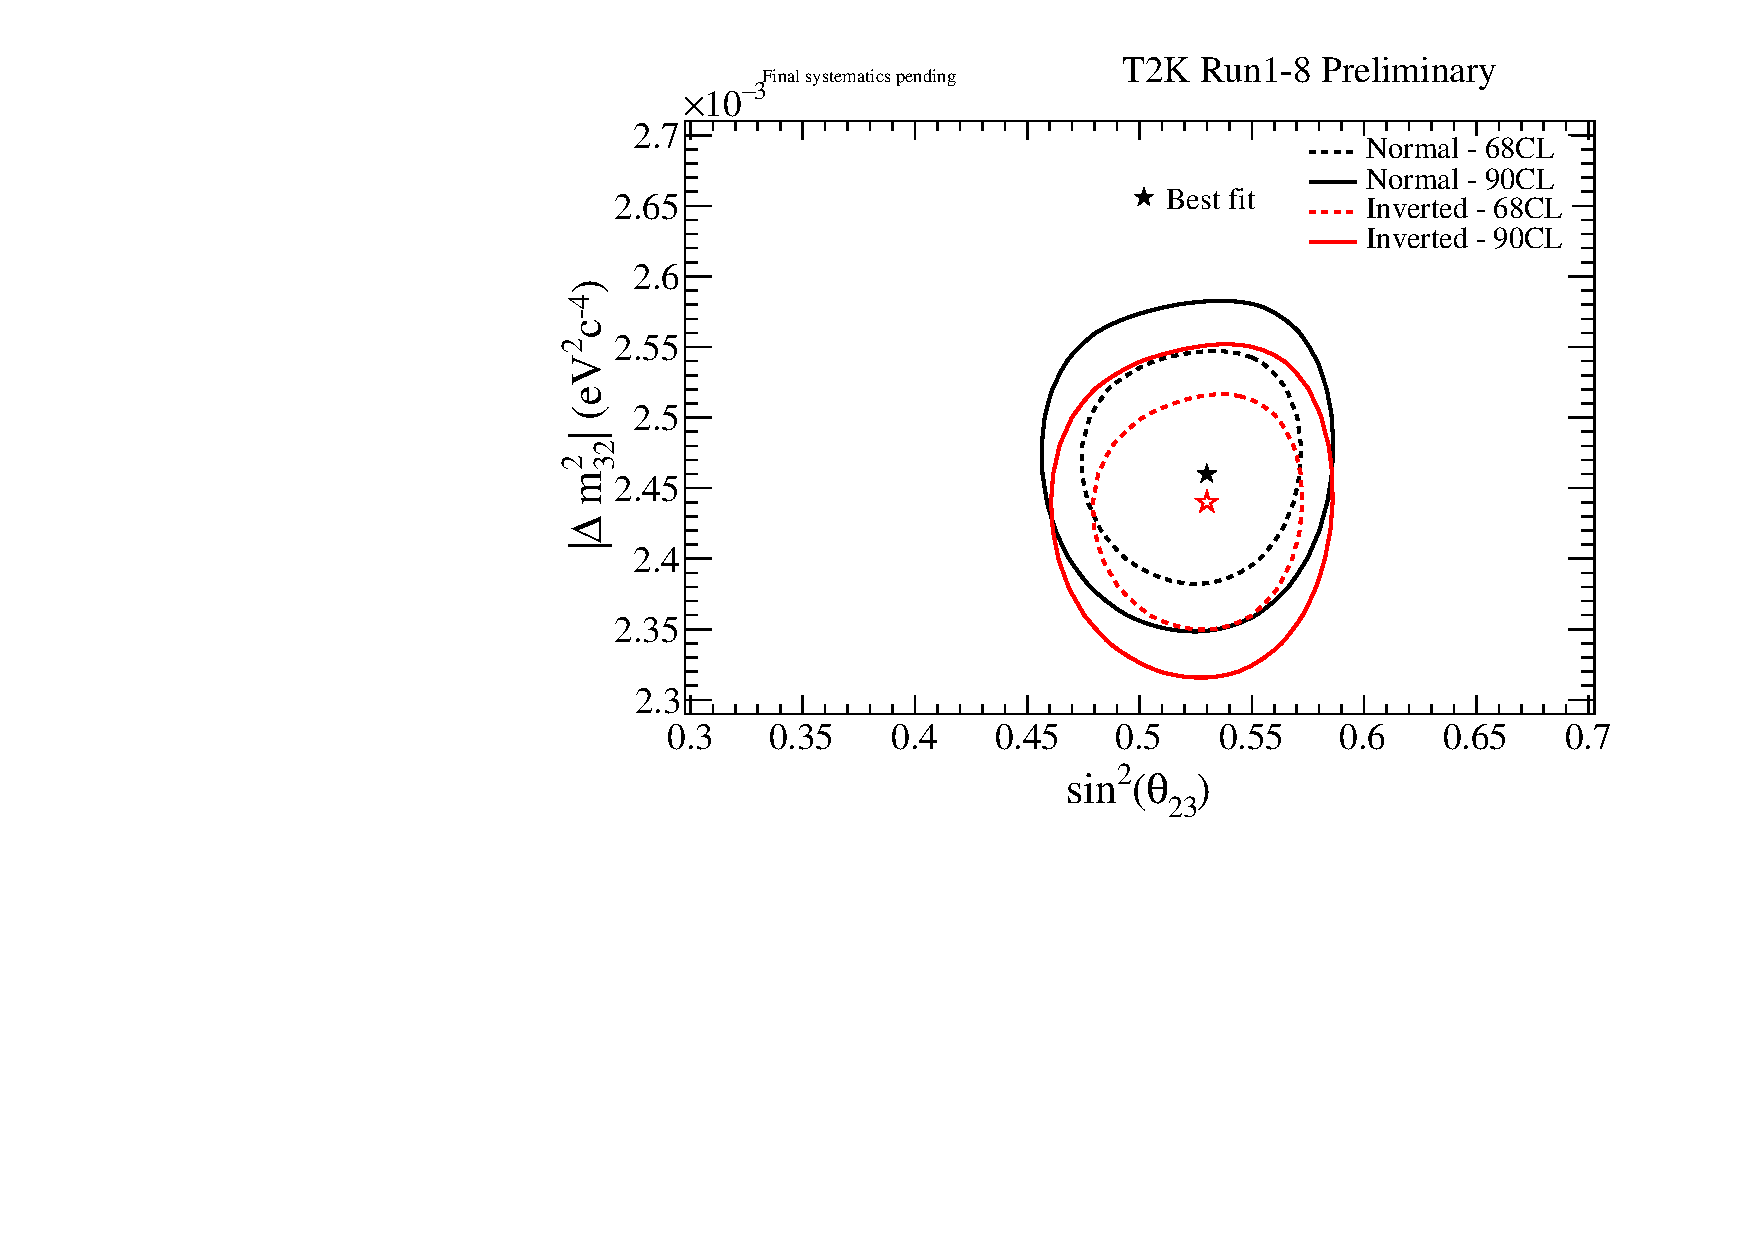
\includegraphics[width=0.9\textwidth]{data/reactor/mixing23_dmsq23_data_reactor_global}
		\caption{\disappearance with reactor constraint}
	\end{subfigure}
	\begin{subfigure}[b]{0.49\textwidth}
		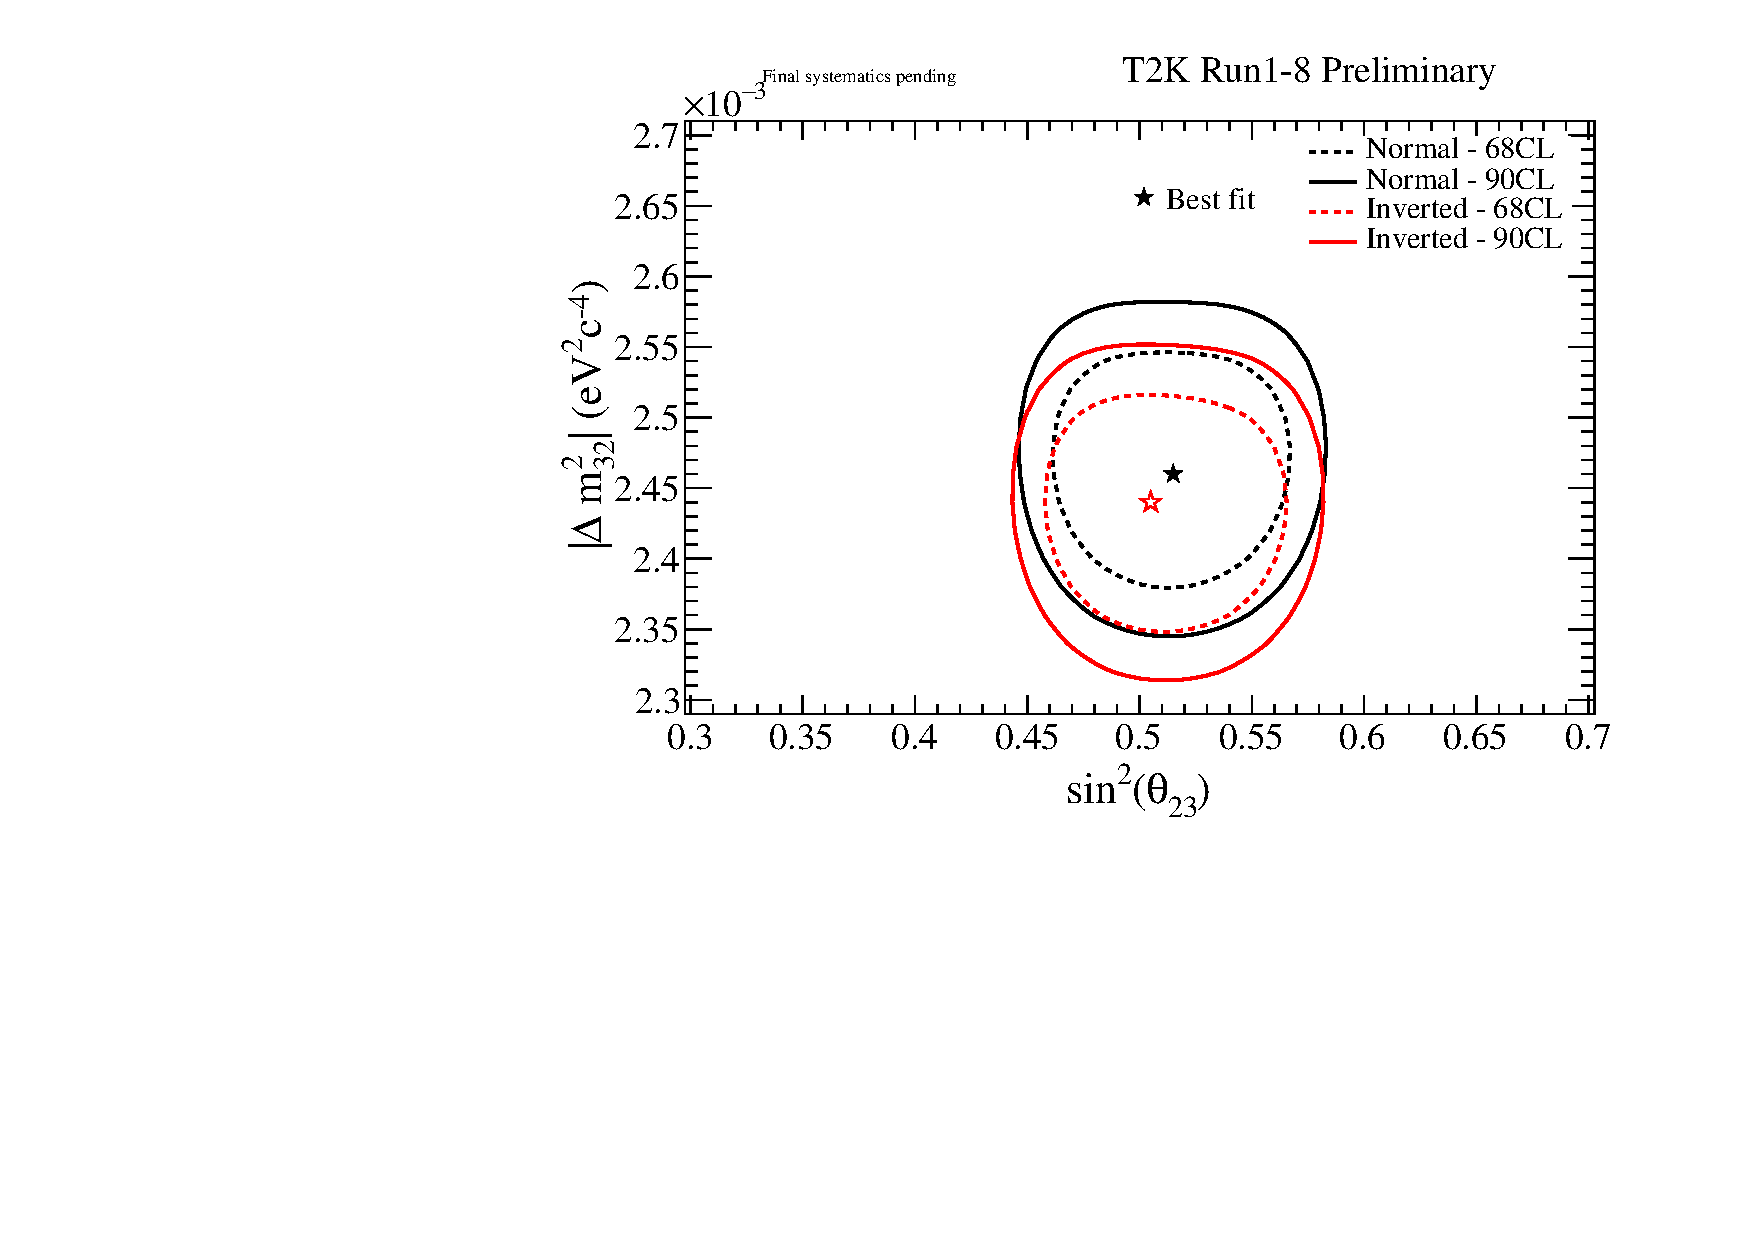
\includegraphics[width=0.9\textwidth]{data/t2k/mixing23_dmsq23_data_t2k_global}
		\caption{\disappearance T2K only}
	\end{subfigure}
	\caption {
		Contours at 68\% and 90\% CL for \disappearance with and without reactor constraint. Normal and inverted hierarchy contours are independent. All 5 samples were used to produce these fits.
	}
	\label{fig:ssqth23_vs_dmsq23_data}
\end{figure*}

\clearpage

\subsection{Results for \deltacp}

The result for \deltacp with reactor constraint and T2K only is shown in fig.~\ref{fig:dcp_data}.

\begin{figure*}[htb]
	\center
	\begin{subfigure}[b]{0.49\textwidth}
		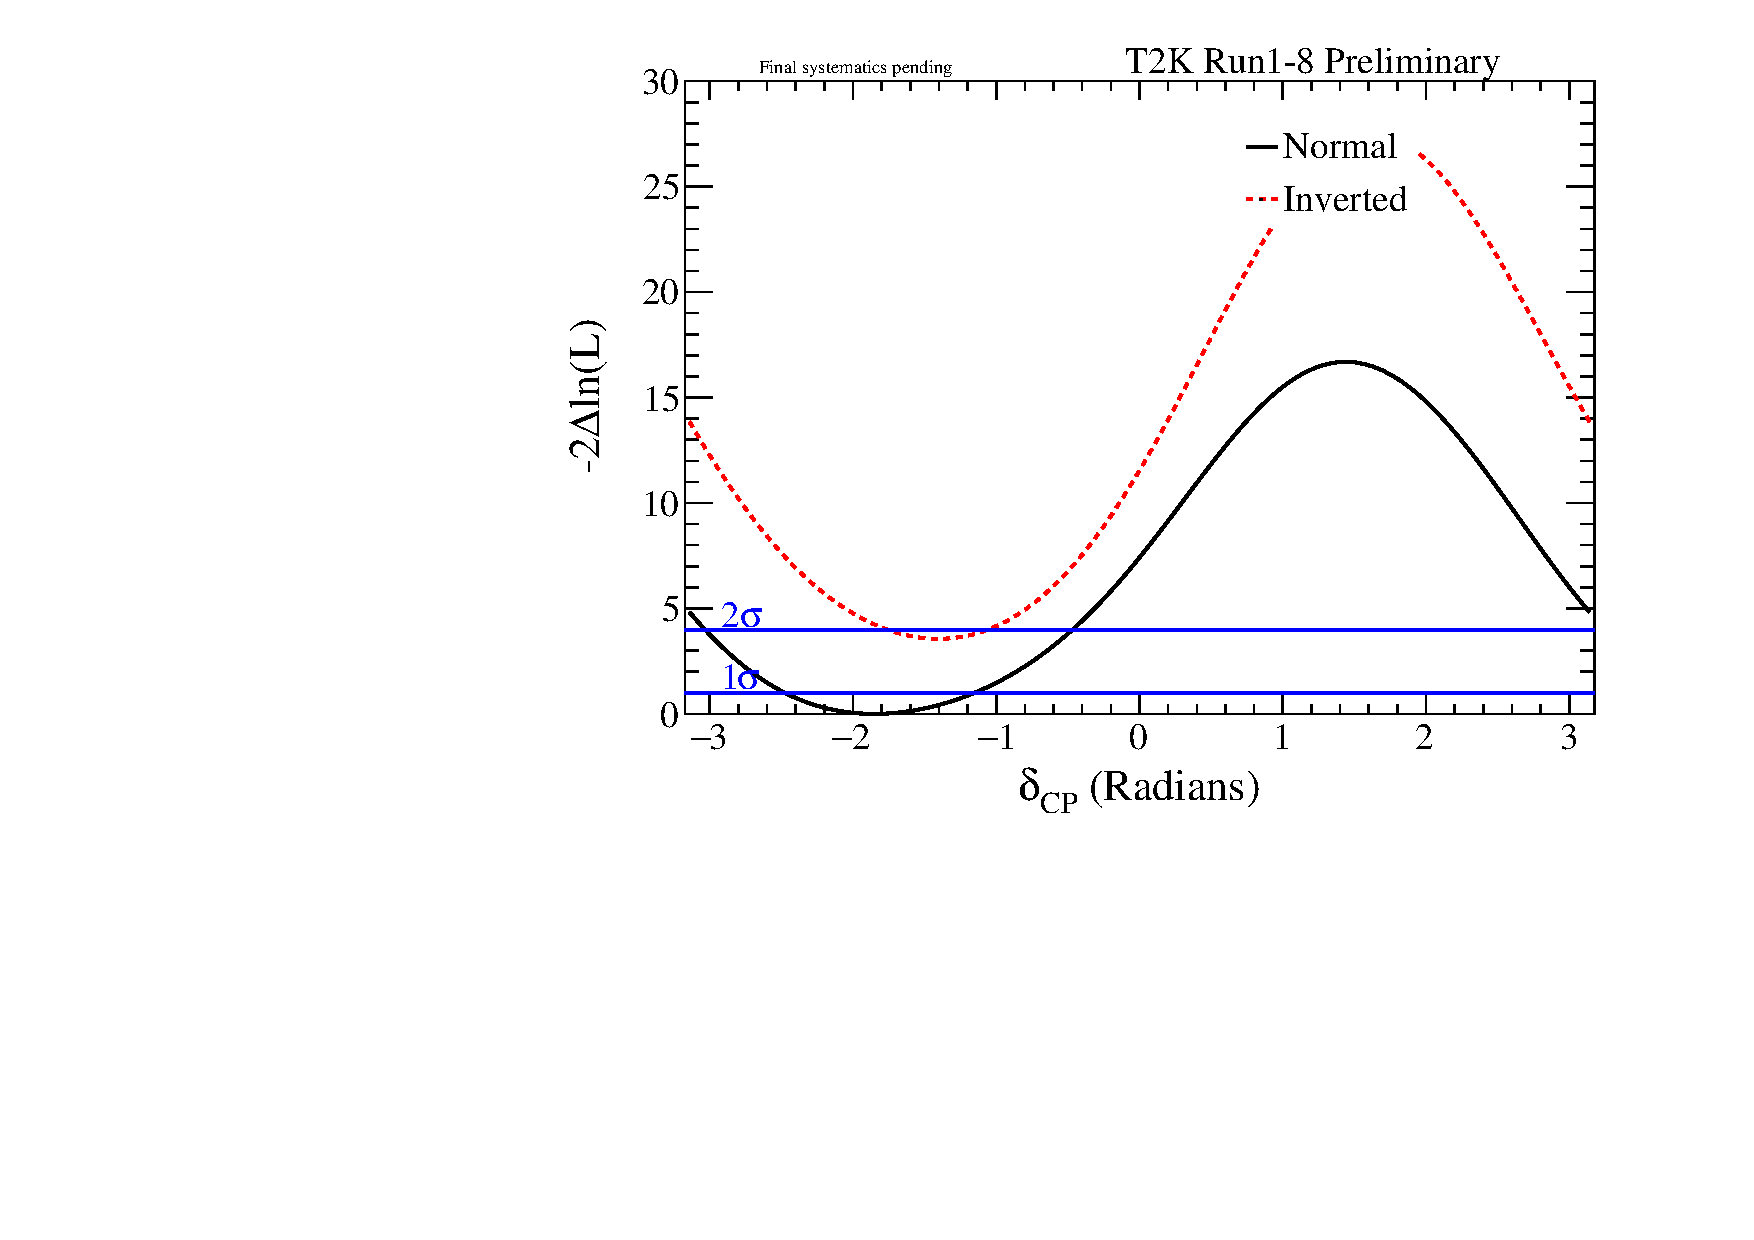
\includegraphics[width=0.9\textwidth]{data/reactor/deltacp_data_reactor_global}
		\caption{\deltacp with reactor constraint}
	\end{subfigure}
	\begin{subfigure}[b]{0.49\textwidth}
		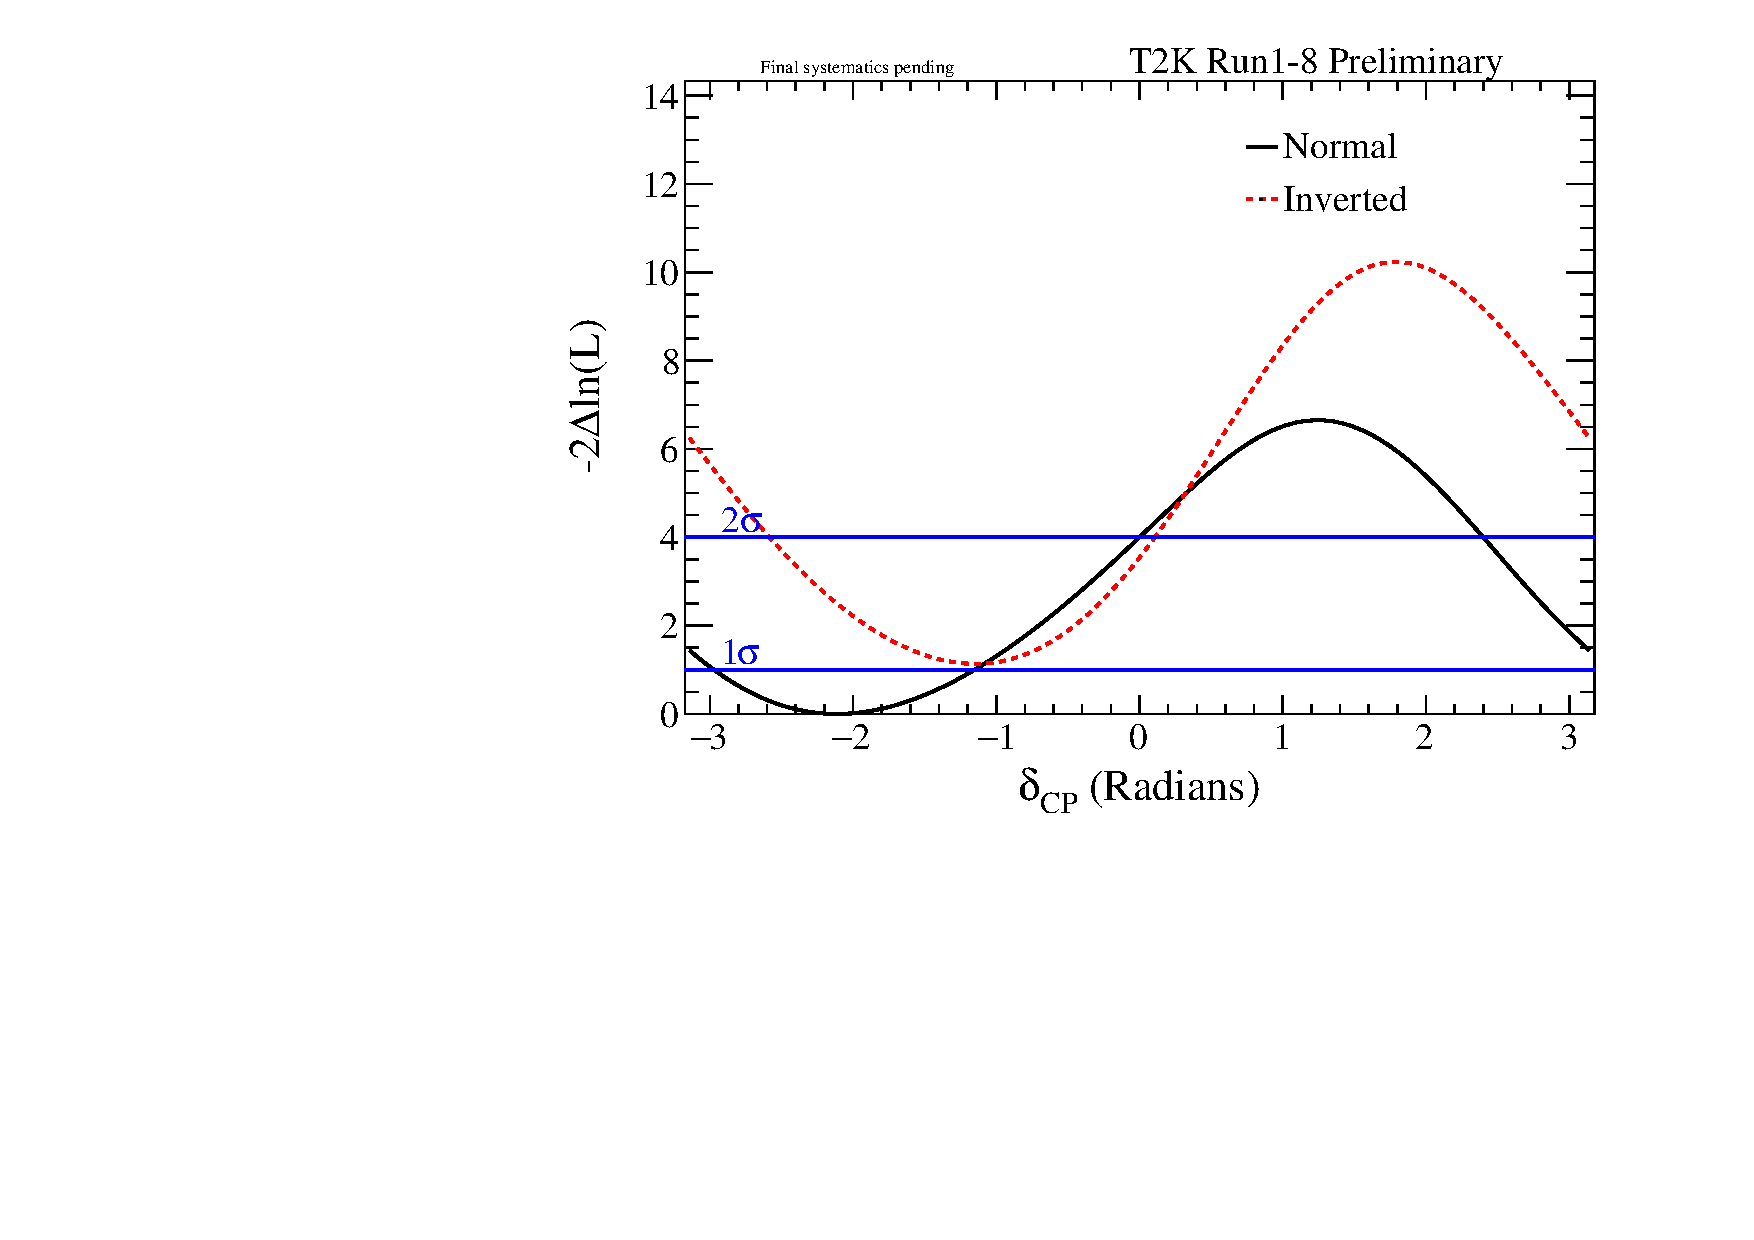
\includegraphics[width=0.9\textwidth]{data/t2k/deltacp_data_t2k_global}
		\caption{\deltacp T2K only}
	\end{subfigure}
	\caption {
		The expected $\Delta\chi^2$ distribution as a function of \deltacp with and without reactor constraint. The mass hierarchy is minimized, with normal and inverted hierarchy $\Delta\chi^2$ distributions shifted to the same global best-fit $\chi^2$ value, which is taken to be the minimum between normal and inverted hierarchy. All 5 samples were used to produce these fits.
	}
	\label{fig:dcp_data}
\end{figure*}

\subsection{Results for \ssqthonethree}

The result for \ssqthonethree (without reactor constraint) is shown in fig.~\ref{fig:th13_data}.

\begin{figure*}[htb]
	\center
	\begin{subfigure}[b]{0.49\textwidth}
		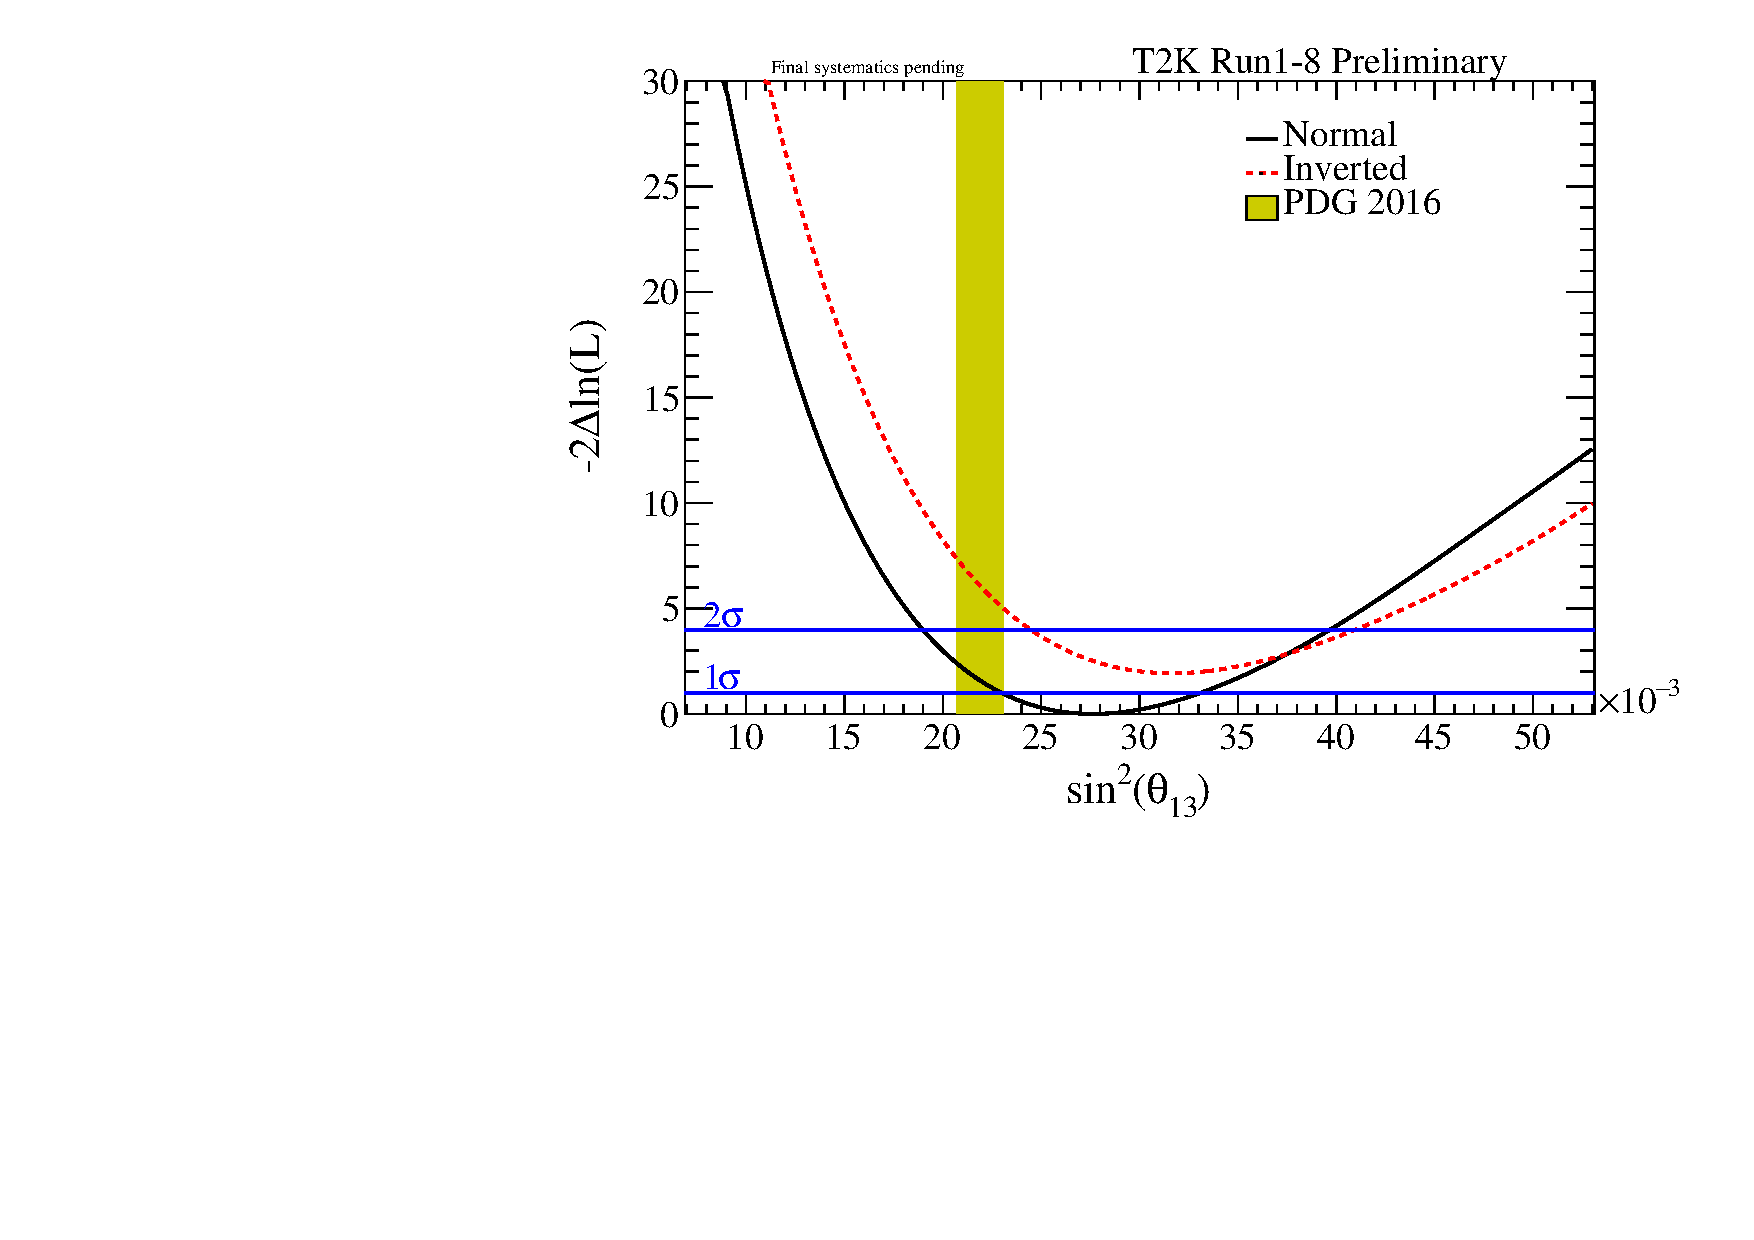
\includegraphics[width=0.9\textwidth]{data/t2k/mixing13_data_t2k_global}
		\caption{\ssqthonethree T2K only}
	\end{subfigure}
	\caption {
		The expected $\Delta\chi^2$ distribution as a function of \ssqthonethree without reactor constraint. The mass hierarchy is minimized, with normal and inverted hierarchy $\Delta\chi^2$ distributions shifted to the same global best-fit $\chi^2$ value, which is taken to be the minimum between normal and inverted hierarchy. All 5 samples were used to produce these fits.
	}
	\label{fig:th13_data}
\end{figure*}

\clearpage

\subsection{Results for \ssqthtwothree}

The result for \ssqthtwothree with reactor constraint and T2K only is shown in fig.~\ref{fig:th23_data}.

\begin{figure*}[htb]
	\center
	\begin{subfigure}[b]{0.49\textwidth}
		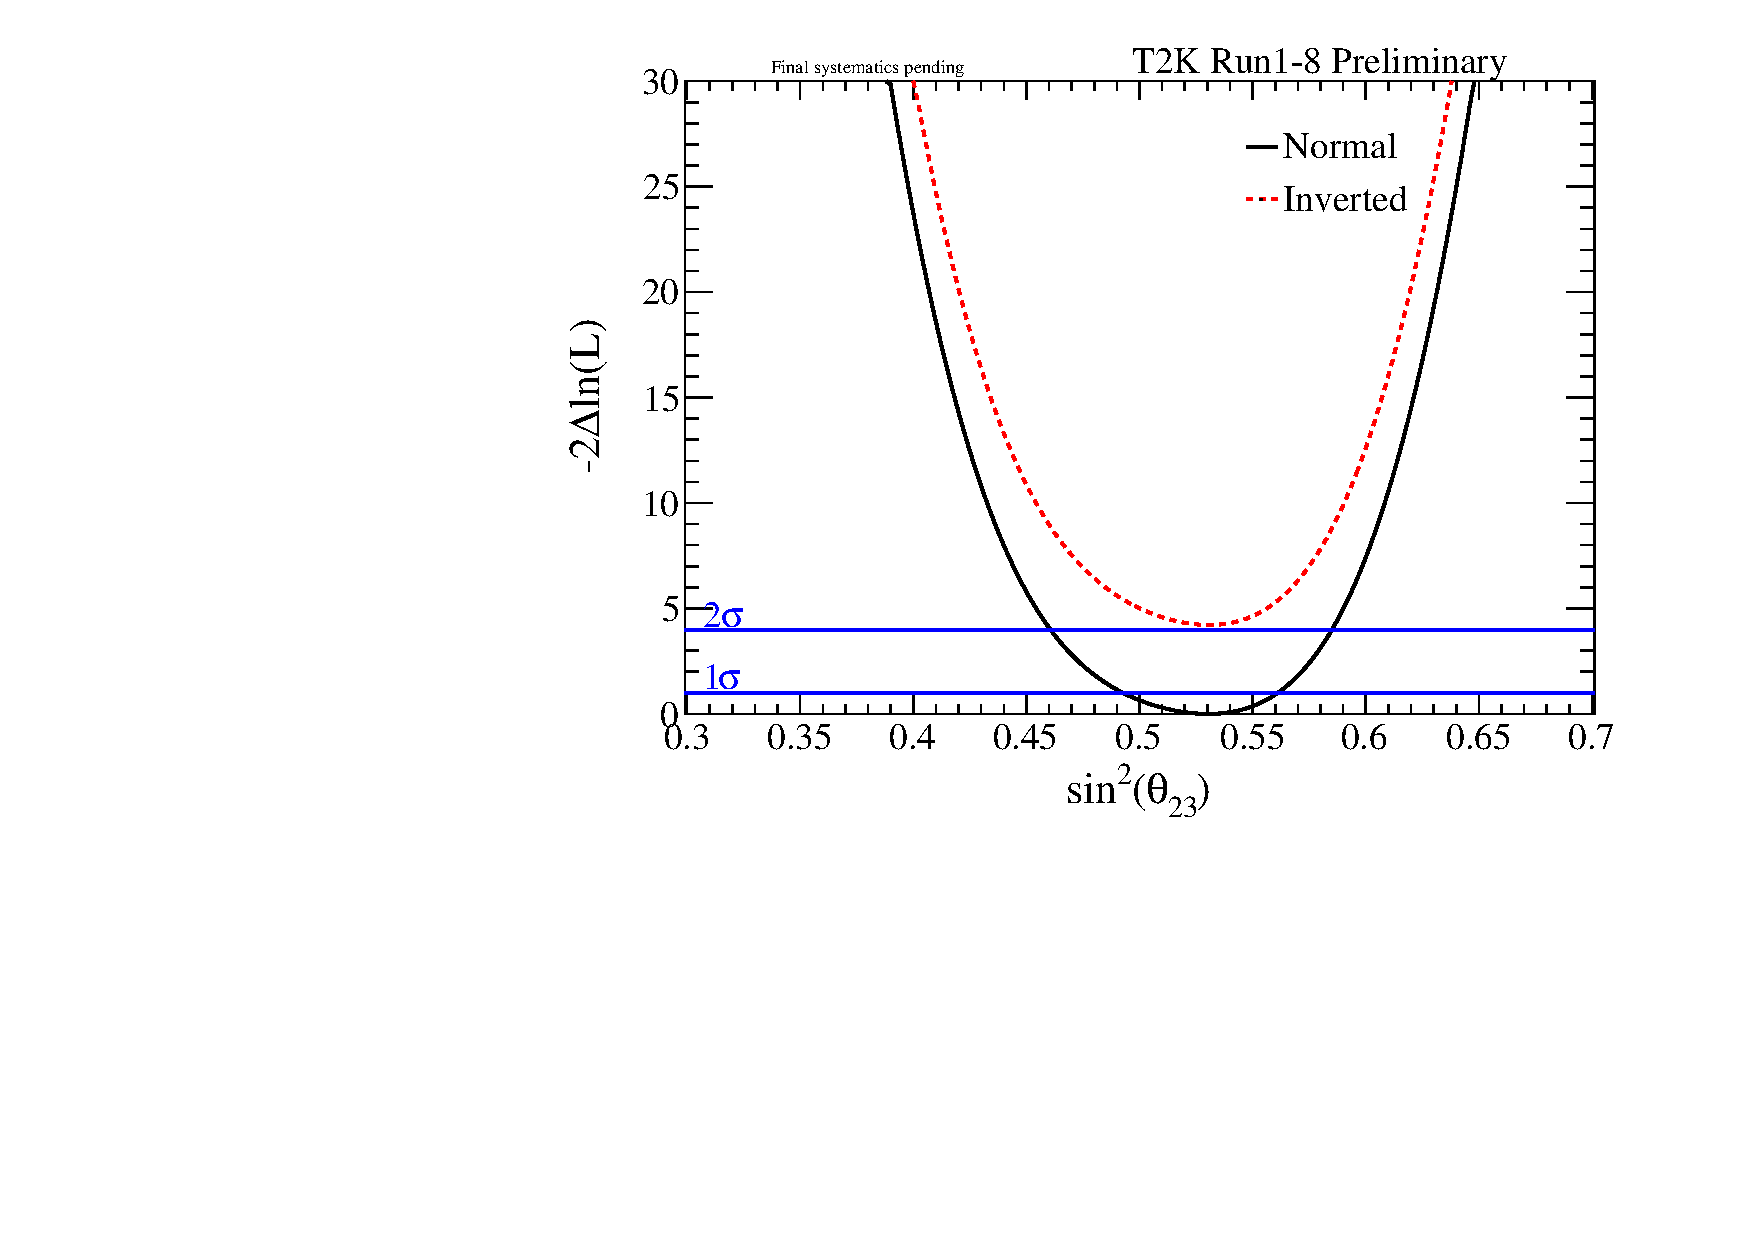
\includegraphics[width=0.9\textwidth]{data/reactor/mixing23_data_reactor_global}
		\caption{\ssqthtwothree with reactor constraint}
	\end{subfigure}
	\begin{subfigure}[b]{0.49\textwidth}
		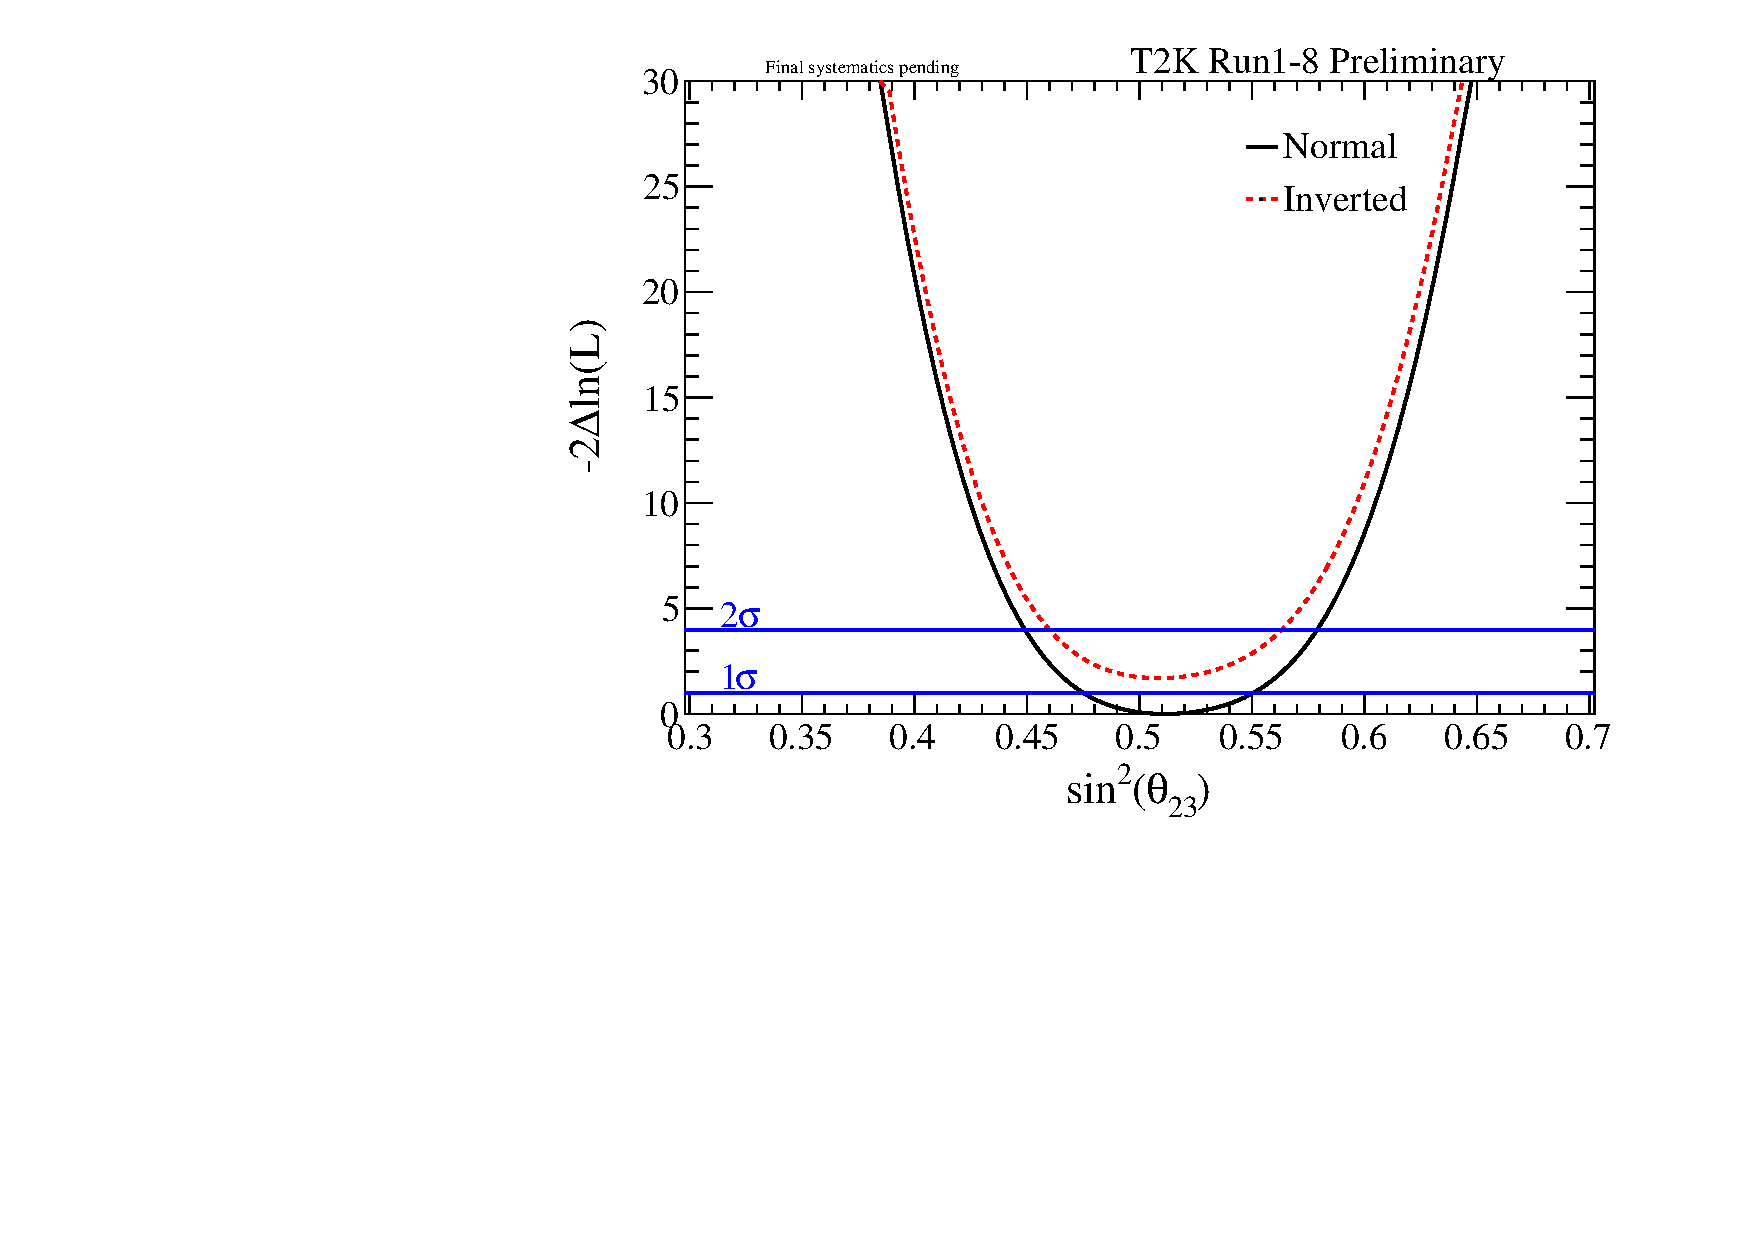
\includegraphics[width=0.9\textwidth]{data/t2k/mixing23_data_t2k_global}
		\caption{\ssqthtwothree T2K only}
	\end{subfigure}
	\caption {
		The expected $\Delta\chi^2$ distribution as a function of \ssqthtwothree with and without reactor constraint. The mass hierarchy is minimized, with normal and inverted hierarchy $\Delta\chi^2$ distributions shifted to the same global best-fit $\chi^2$ value, which is taken to be the minimum between normal and inverted hierarchy. All 5 samples were used to produce these fits.
	}
	\label{fig:th23_data}
\end{figure*}

\subsection{Results for \dmsqtwothree}

The result for \dmsqtwothree with reactor constraint and T2K only is shown in fig.~\ref{fig:dmsq23_data}.

\begin{figure*}[htb]
	\center
	\begin{subfigure}[b]{0.49\textwidth}
		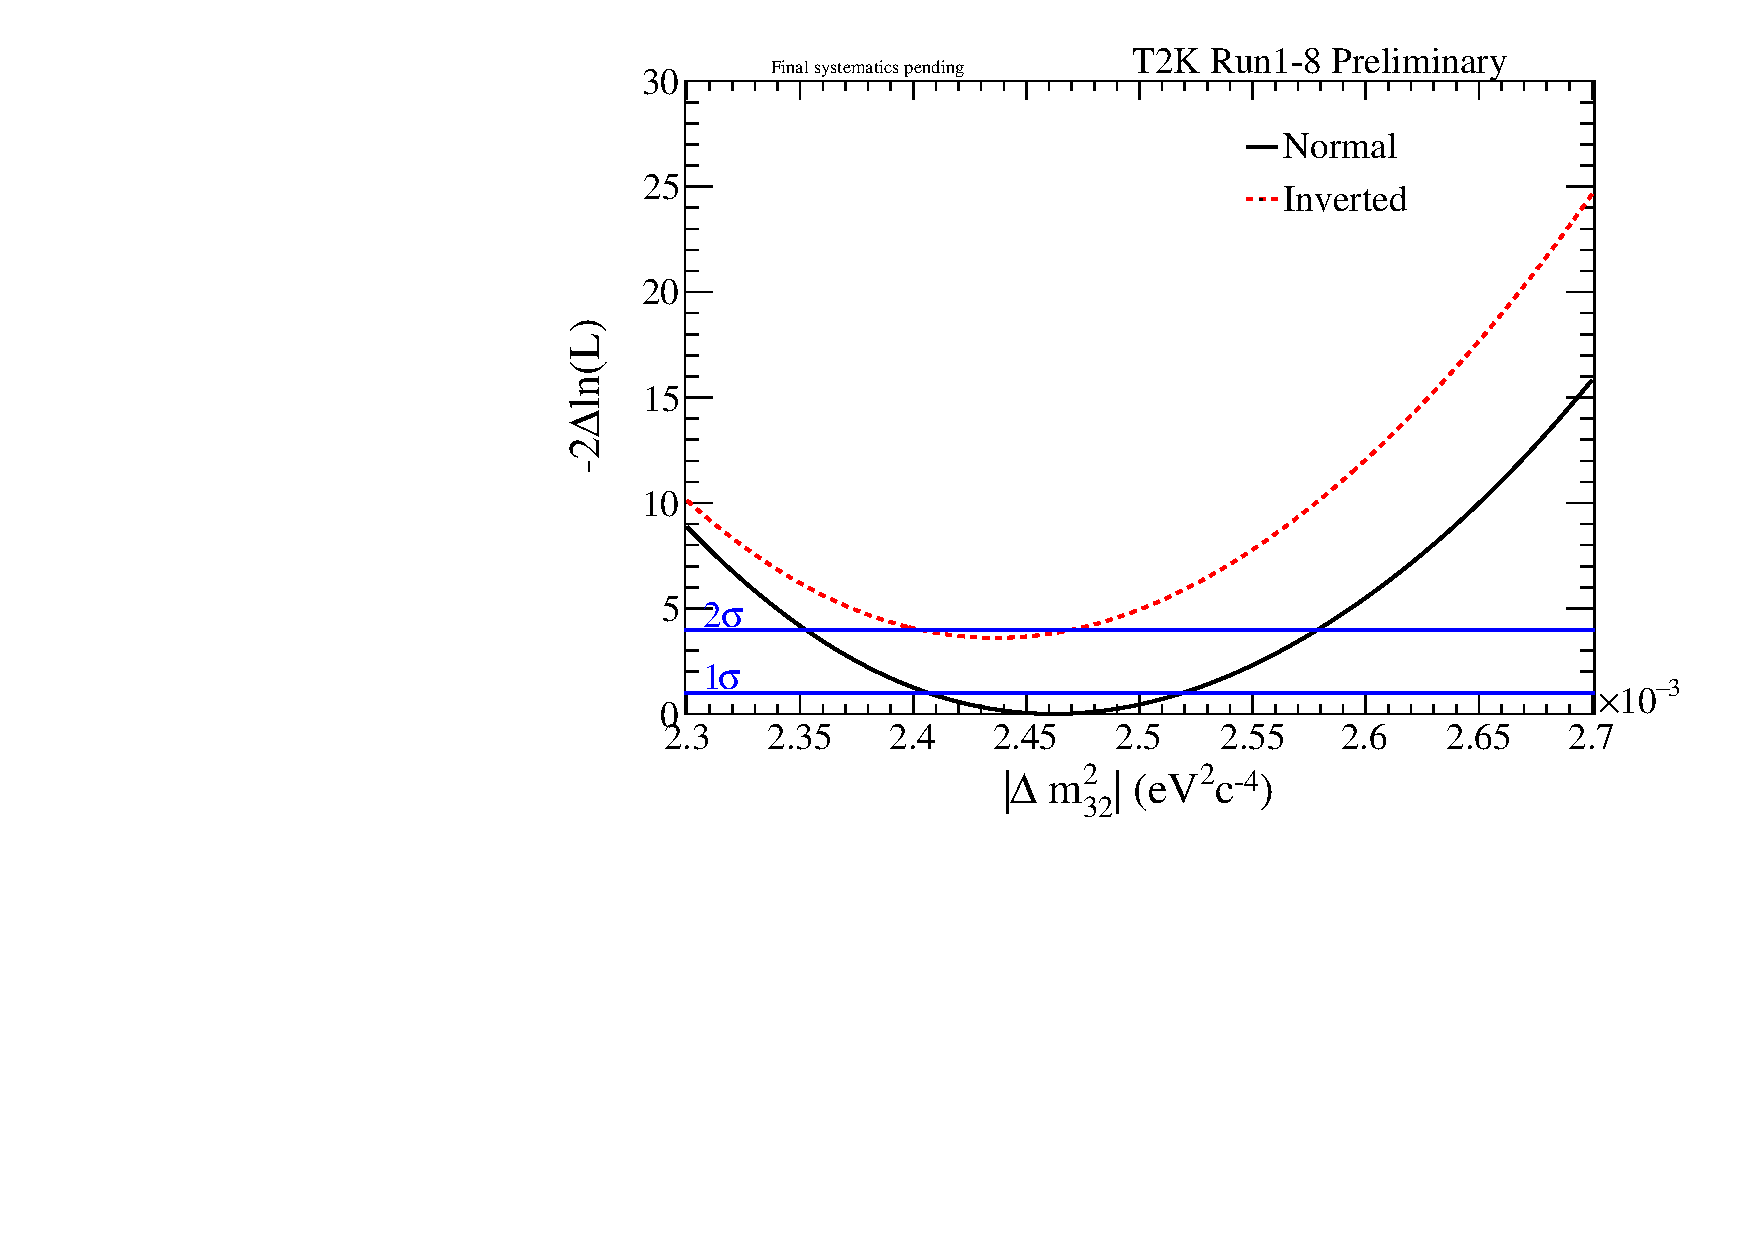
\includegraphics[width=0.9\textwidth]{data/reactor/dmsq23_data_reactor_global}
		\caption{\dmsqtwothree with reactor constraint}
	\end{subfigure}
	\begin{subfigure}[b]{0.49\textwidth}
		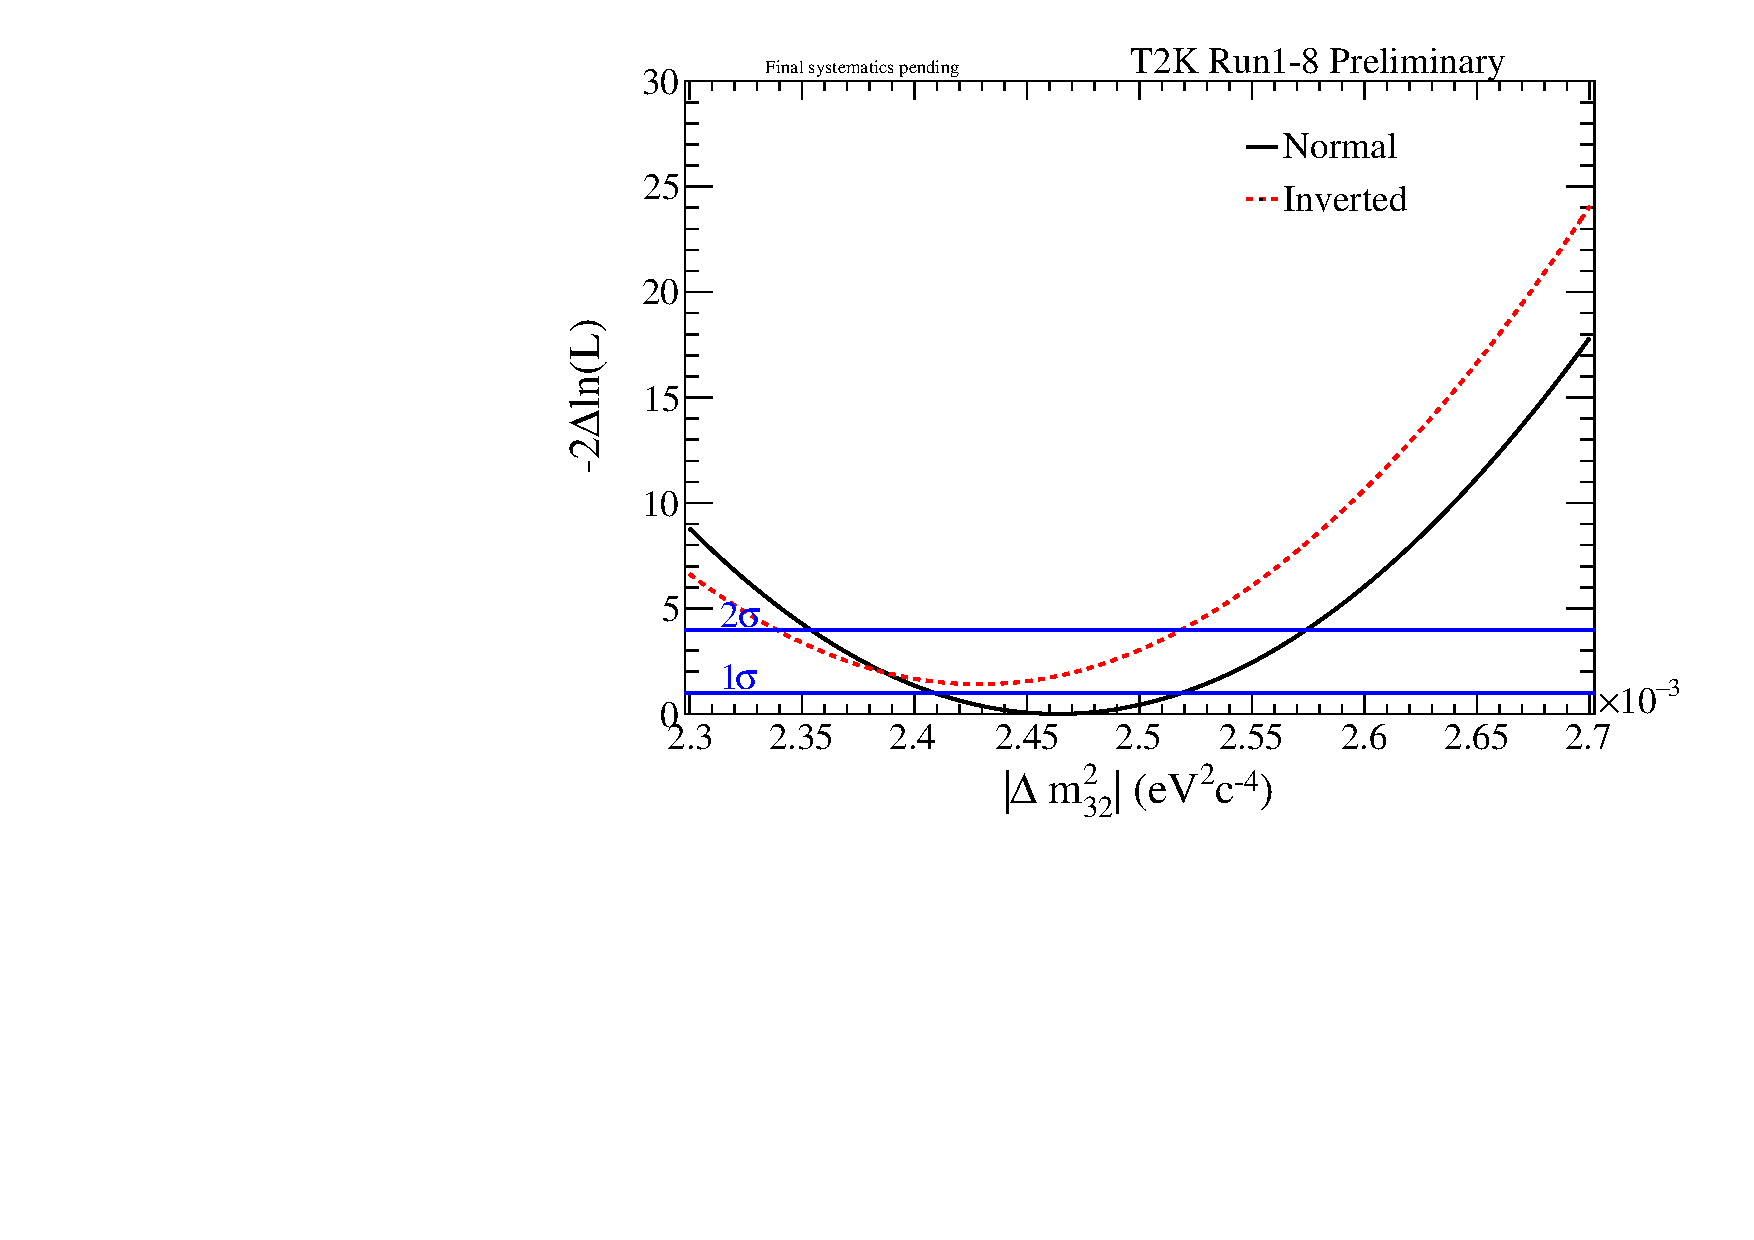
\includegraphics[width=0.9\textwidth]{data/t2k/dmsq23_data_t2k_global}
		\caption{\dmsqtwothree T2K only}
	\end{subfigure}
	\caption {
		The expected $\Delta\chi^2$ distribution as a function of \dmsqtwothree with and without reactor constraint. The mass hierarchy is minimized, with normal and inverted hierarchy $\Delta\chi^2$ distributions shifted to the same global best-fit $\chi^2$ value, which is taken to be the minimum between normal and inverted hierarchy. All 5 samples were used to produce these fits.
	}
	\label{fig:dmsq23_data}
\end{figure*}

\subsection {Feldman-Cousins simultaneous fit of \deltacp and mass hierarchy}
\label{sec:fc_significance}


This section presents the results of the Feldman-Cousins fit of \deltacp and mass hierarchy. Throws of oscillation parameters are made according to PDG 2016 best-fit values and errors for \ssqthonethree, \ssqthonetwo and \dmsqonetwo, whilst \ssqthtwothree and \dmsqtwothree are thrown according to the likelihood distribution produced by an Asimov fit using the best-fit from data for these parameters, this is an updated method from the previous analysis and the proposal is given in \cite{NewFC}. \deltacp is fixed at one of 9 evenly specified values on the range $\left[-\pi,\pi\right]$.

\subsubsection{Input oscillation parameters}
\label{sec:fc_significance:inputs}

The distributions of oscillation parameters (for normal hierarchy) are shown in \cref{fig:fc_input_dist}. Note that whilst the distributions of the atmospheric parameters are shown independently they are generated jointly from the likelihood distribution shown in \cref{fig:fc_input_disapp}.

\begin{figure*}[htb]
	\center
	\begin{subfigure}[b]{0.49\textwidth}
		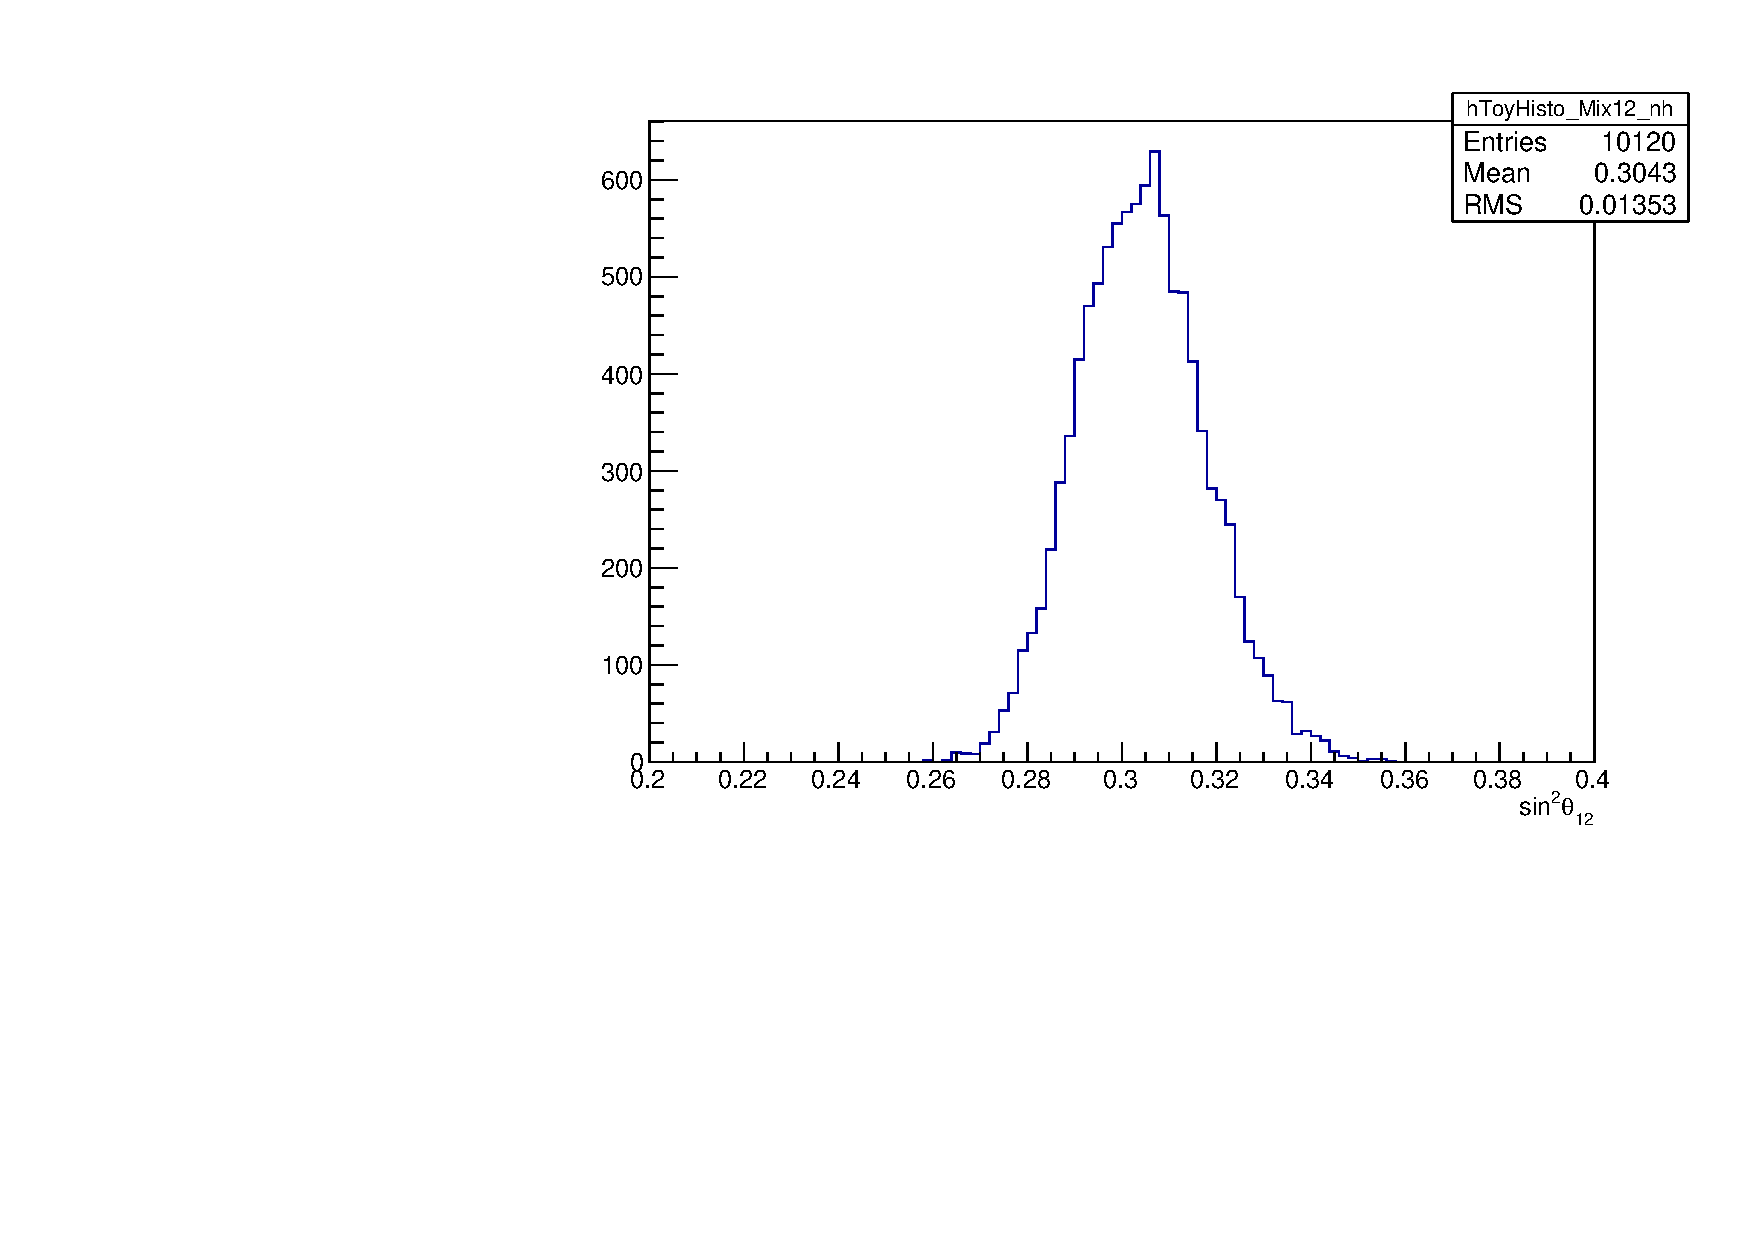
\includegraphics[width=0.9\textwidth]{data/fc/inputs/mixing12_in}
		\caption{\ssqthonetwo}
	\end{subfigure}
	\begin{subfigure}[b]{0.49\textwidth}
		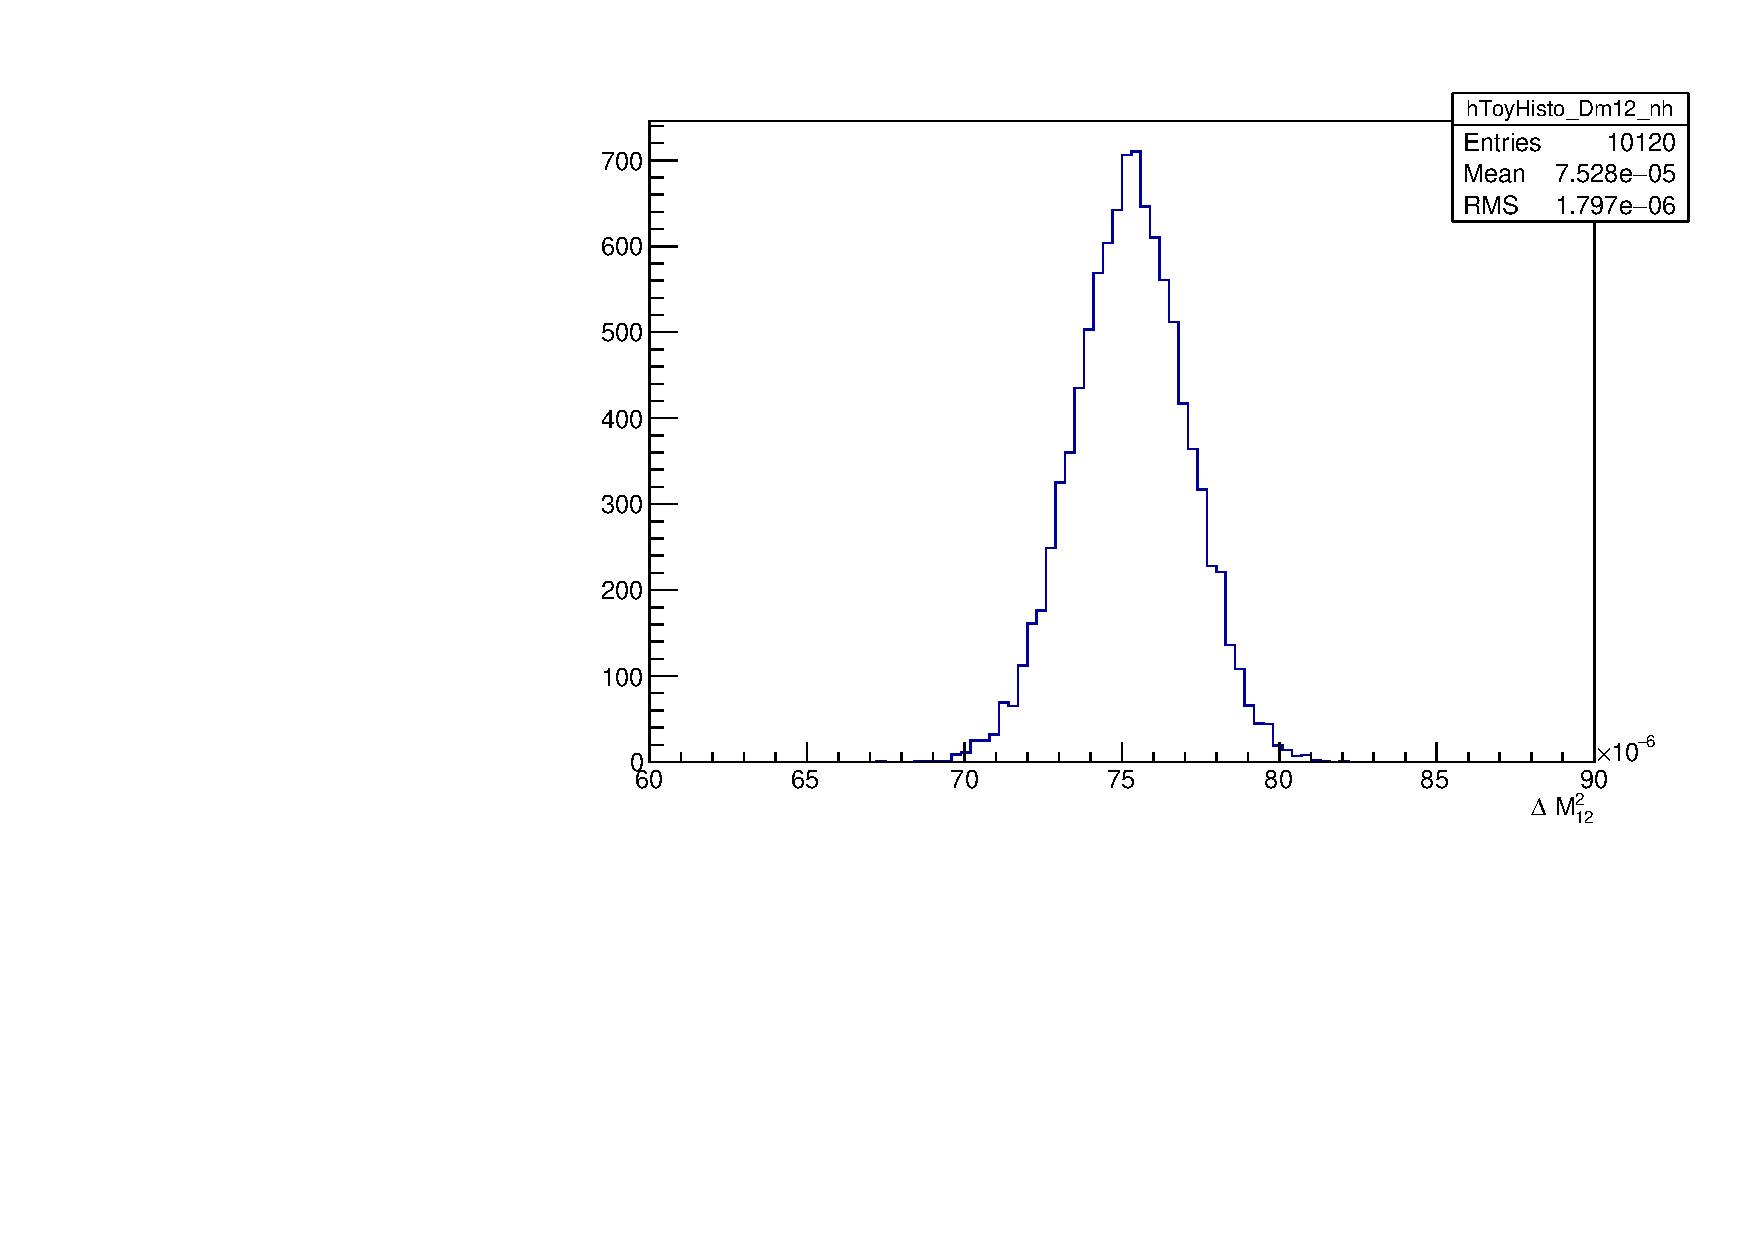
\includegraphics[width=0.9\textwidth]{data/fc/inputs/dm12_in}
		\caption{\dmsqonetwo}
	\end{subfigure}
	\begin{subfigure}[b]{0.49\textwidth}
		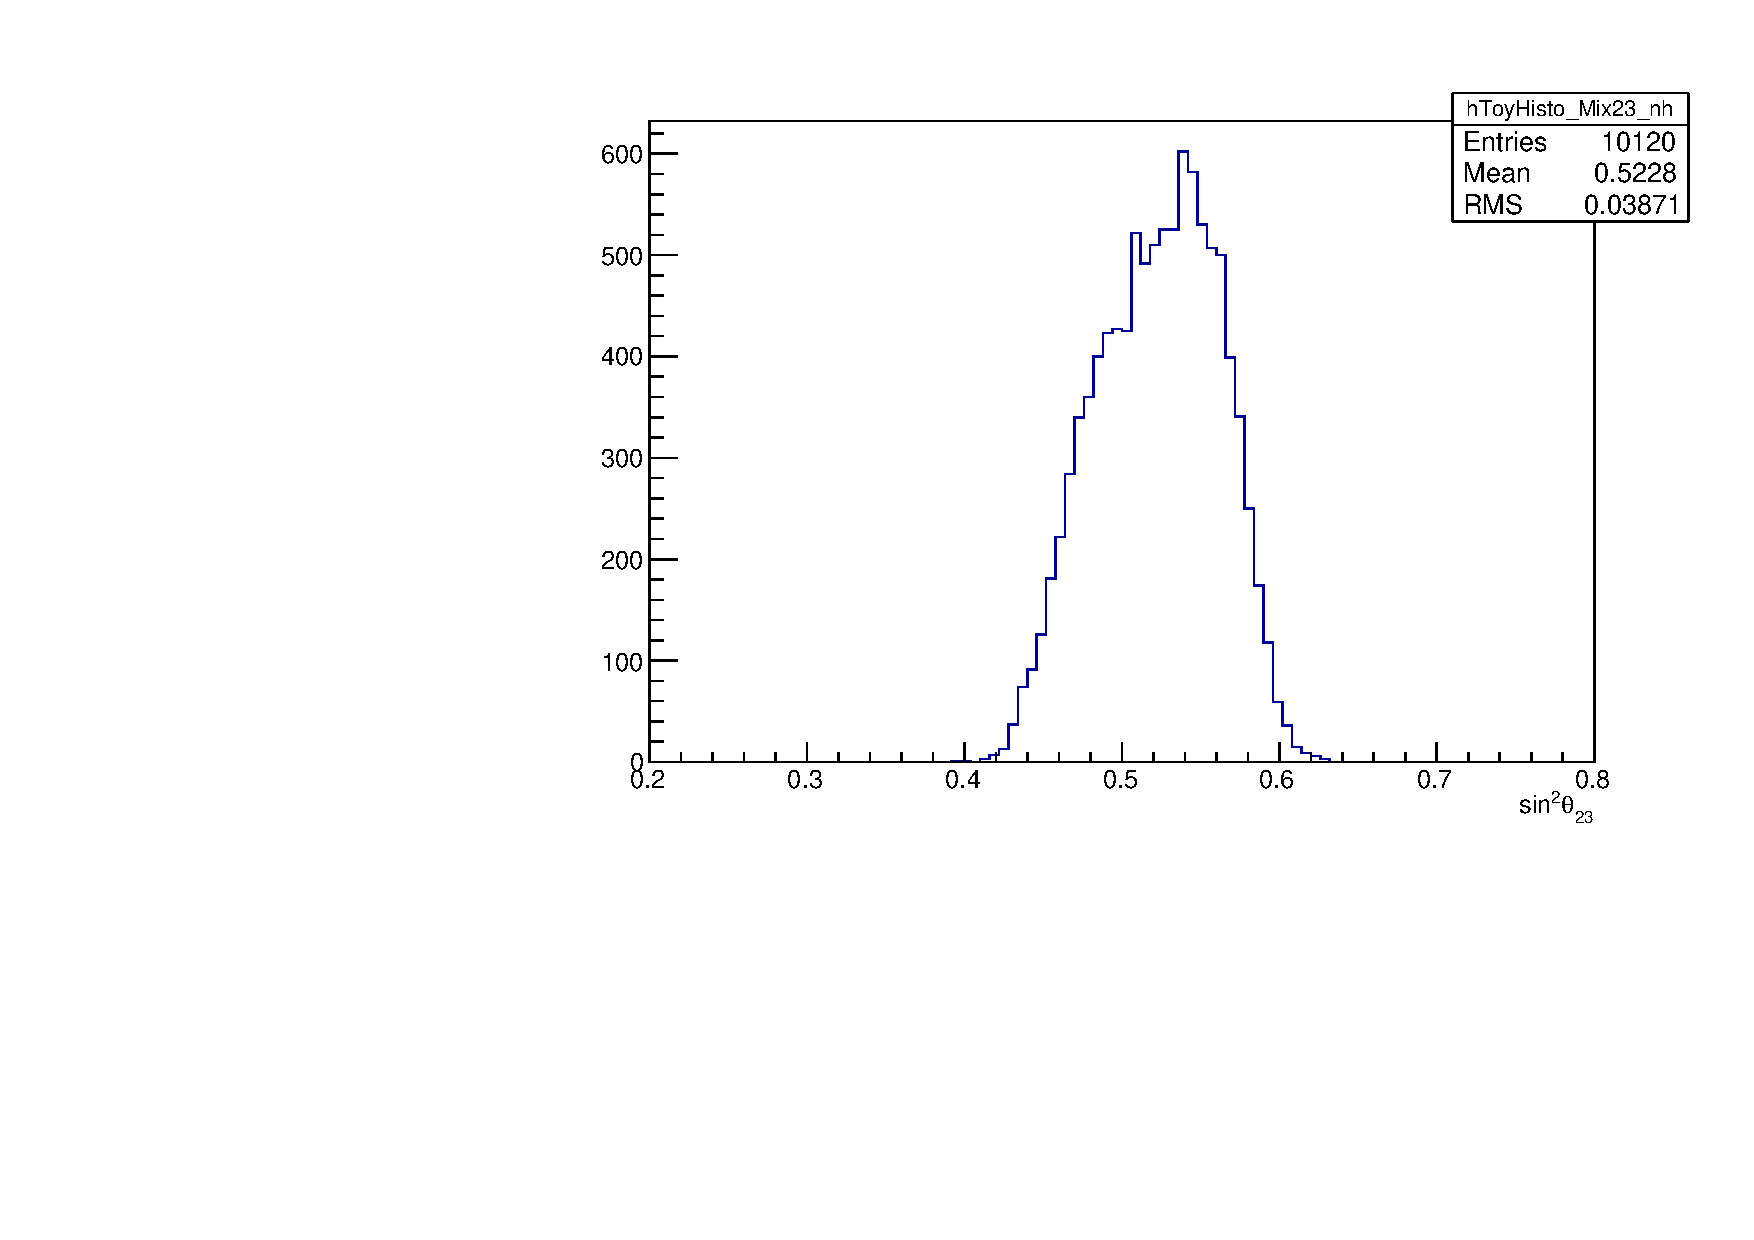
\includegraphics[width=0.9\textwidth]{data/fc/inputs/mixing23_in}
		\caption{\ssqthtwothree}
	\end{subfigure}
	\begin{subfigure}[b]{0.49\textwidth}
		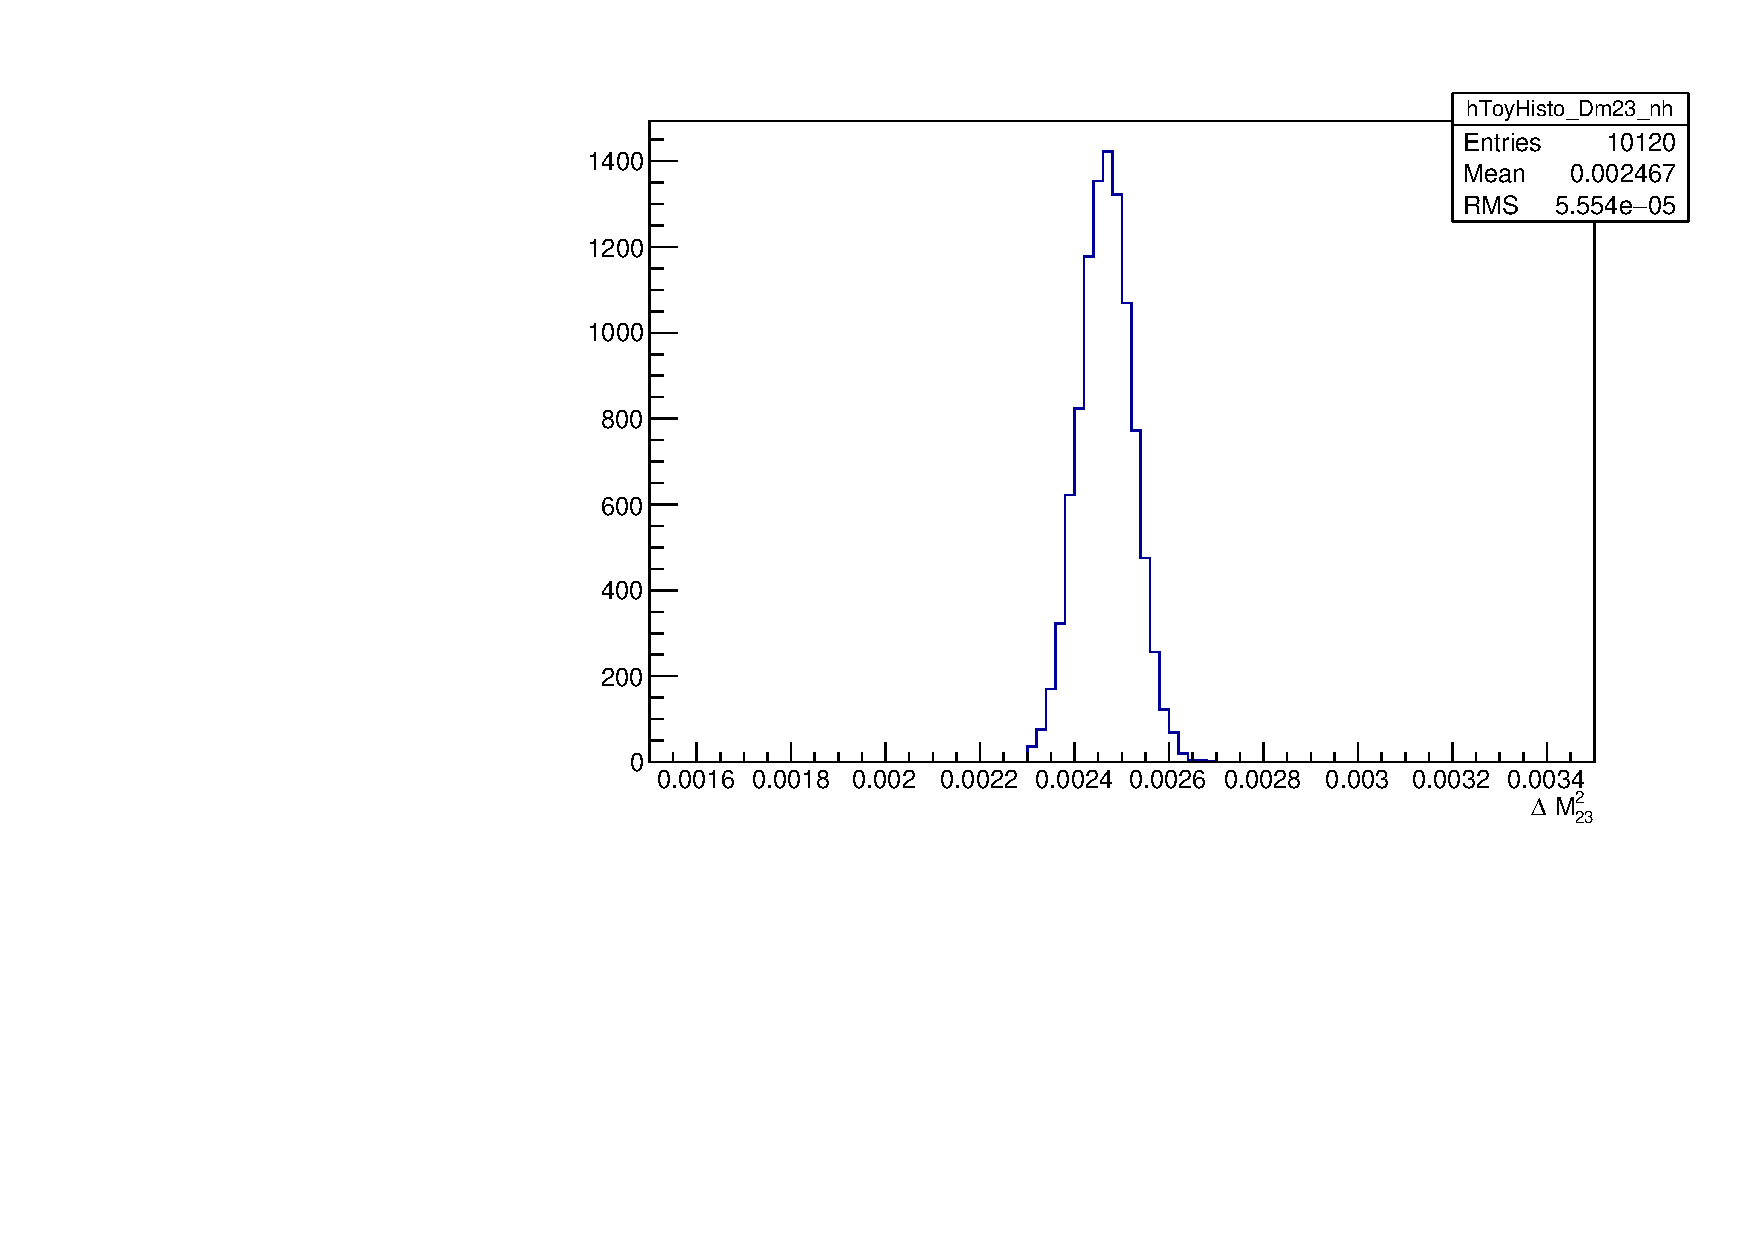
\includegraphics[width=0.9\textwidth]{data/fc/inputs/dm23_in}
		\caption{\dmsqtwothree}
	\end{subfigure}
	\begin{subfigure}[b]{0.49\textwidth}
		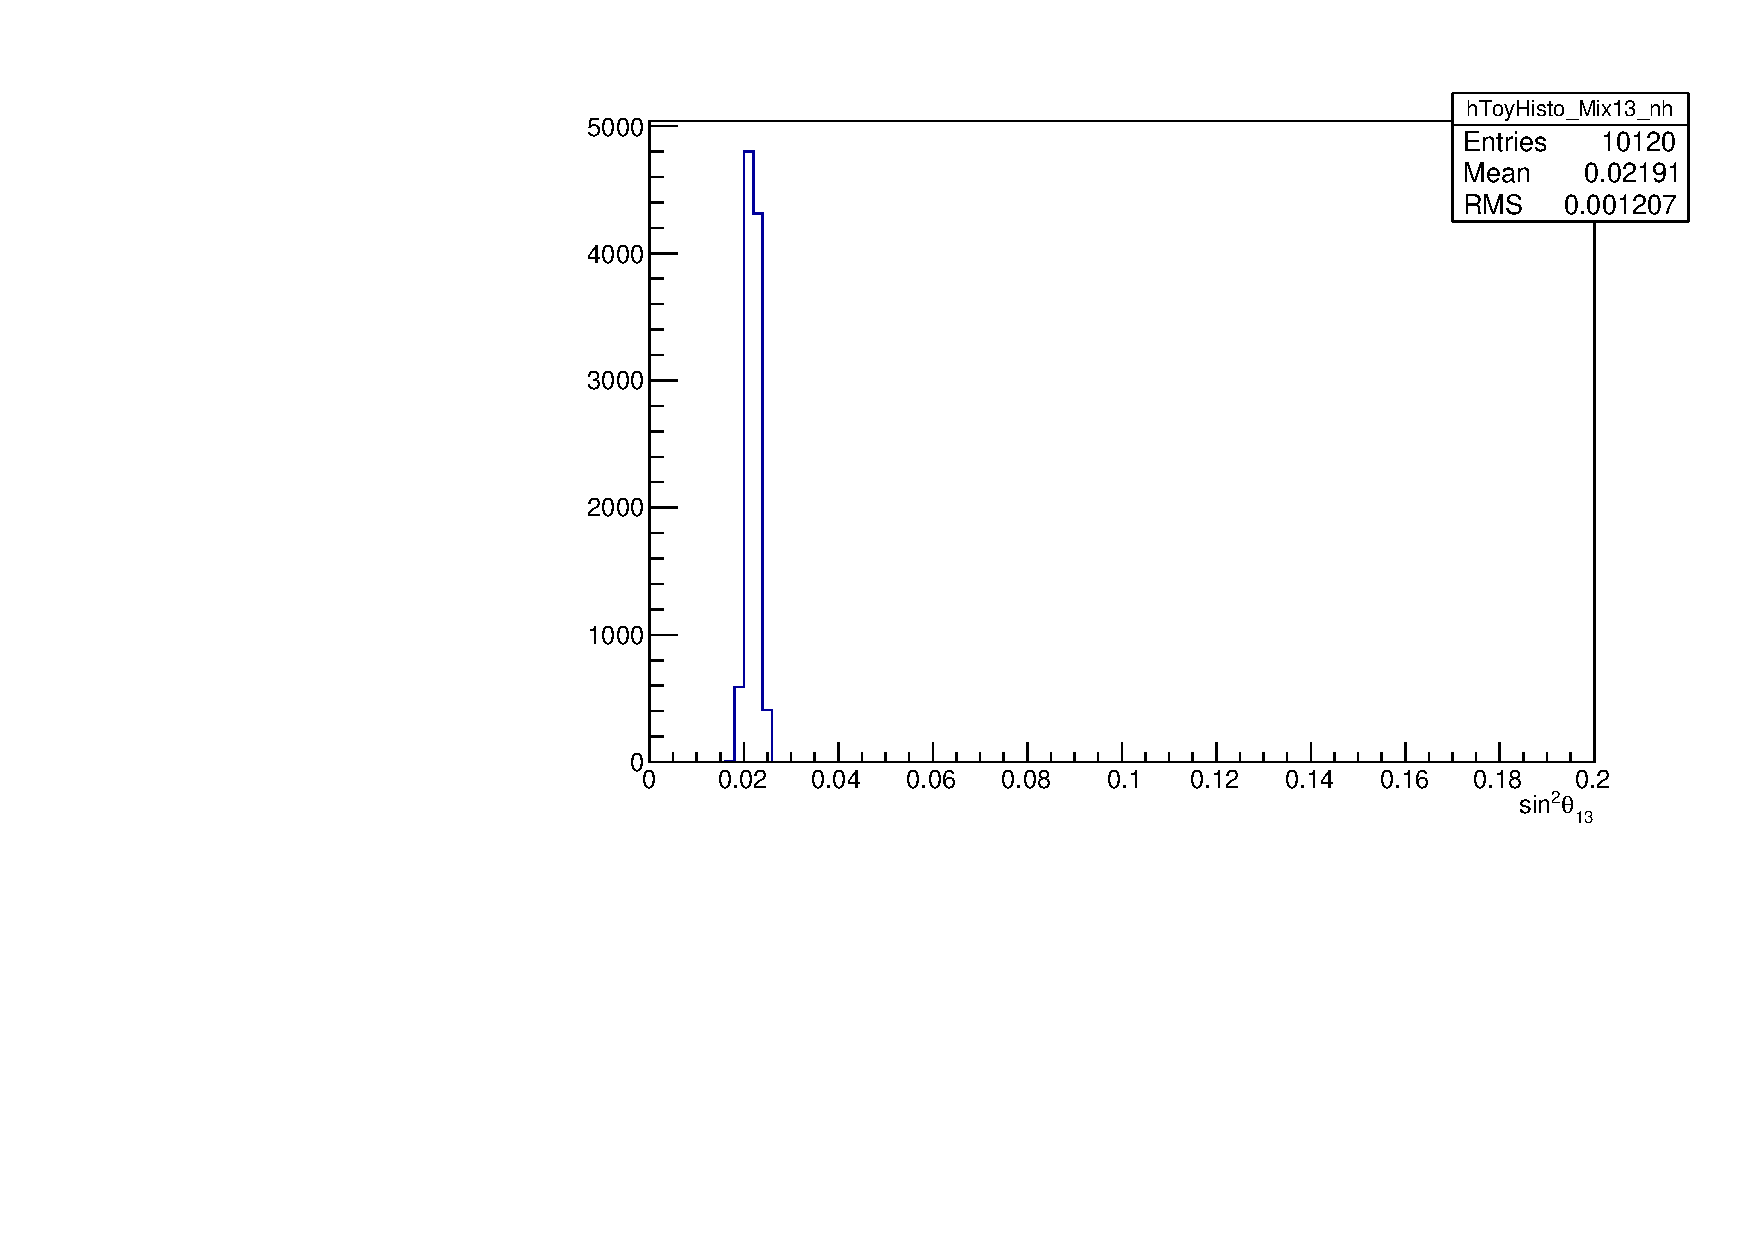
\includegraphics[width=0.9\textwidth]{data/fc/inputs/mixing13_in}
		\caption{\ssqthonethree}
	\end{subfigure}
	\caption {
		Distribution of oscillation parameter throws for Feldman-Cousins fits.
	}
	\label{fig:fc_input_dist}
\end{figure*}

\begin{figure*}[htb]
	\begin{subfigure}[b]{0.49\textwidth}
		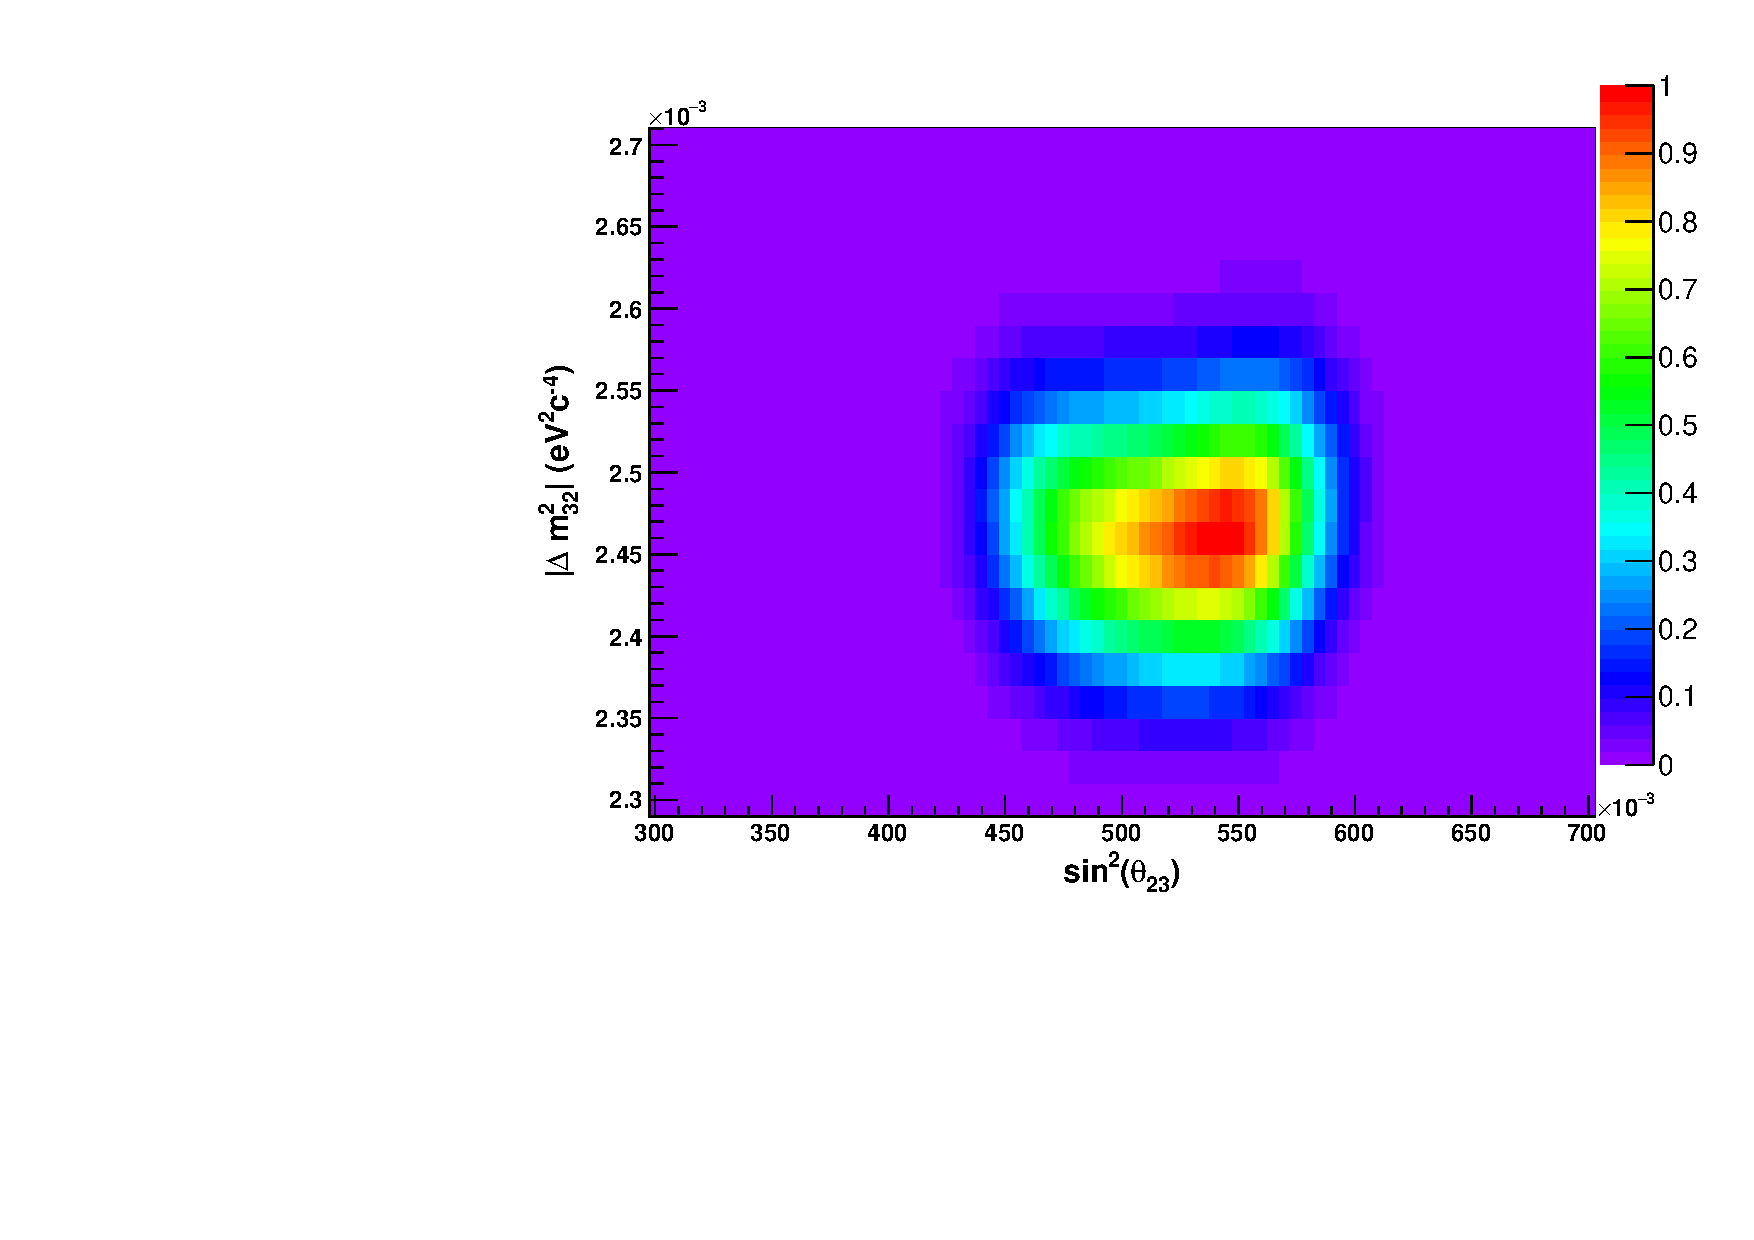
\includegraphics[width=0.9\textwidth]{data/fc/inputs/disappearance_nh_likelihood}
		\caption{Normal hierarchy}
	\end{subfigure}
	\begin{subfigure}[b]{0.49\textwidth}
		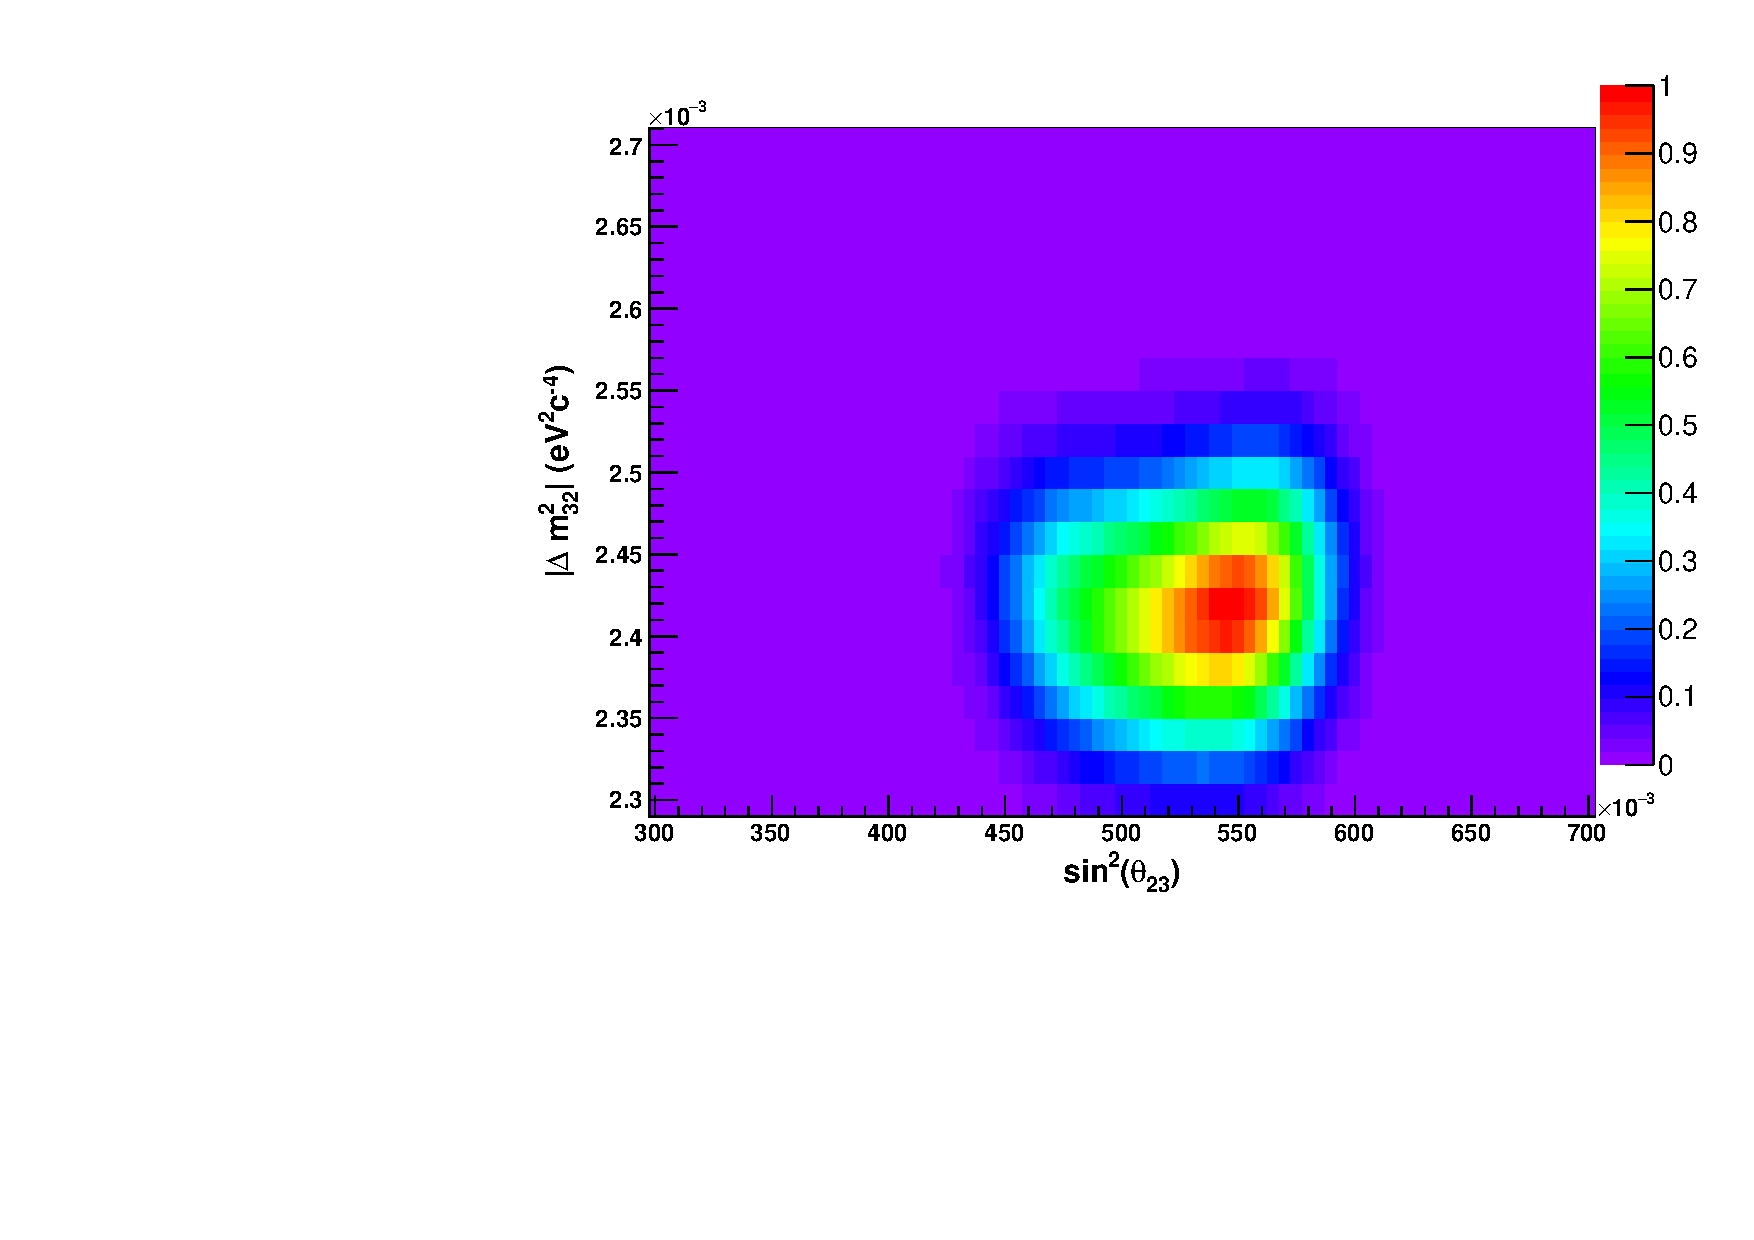
\includegraphics[width=0.9\textwidth]{data/fc/inputs/disappearance_ih_likelihood}
		\caption{Inverted hierarchy}
	\end{subfigure}
	\caption {
		Likelihood surfaces for throws of the disappearance parameter.
	}
	\label{fig:fc_input_disapp}
\end{figure*}

\subsubsection{Feldman-Cousins critical values and confidence intervals}
\label{sec:fc_significance:intervals}

In \cref{fig:fc_interval} the confidence intervals obtained with the `Feldman-Cousins' method are shown for \deltacp and mass hierarchy with reactor constraint for the \RunPeriod data set. The critical values at 90\%, $2\sigma$ and $3\sigma$ CL are computed for both the mass hierarchies at the following true values of \deltacp; $-\pi$, $-3\pi/4$, $-\pi/2$, $-\pi/4$, 0, $+\pi/4$, $+\pi/2$, $+3\pi/4$, and $+\pi$. Inverted hierarchy is almost excluded at $2\sigma$, except for a small interval around $\delta_{CP} = -\pi/2$. Both $\delta_{CP} = 0$ and $\delta_{CP} = \pi$ are excluded at $2\sigma$. In \cref{tab:fc_interval} the $2\sigma$ CL intervals for \deltacp versus mass hierarchy, obtained with the Feldman-Cousins method, are shown.

\begin{figure*}[htb]
	\center
	\begin{subfigure}[b]{0.6\textwidth}
		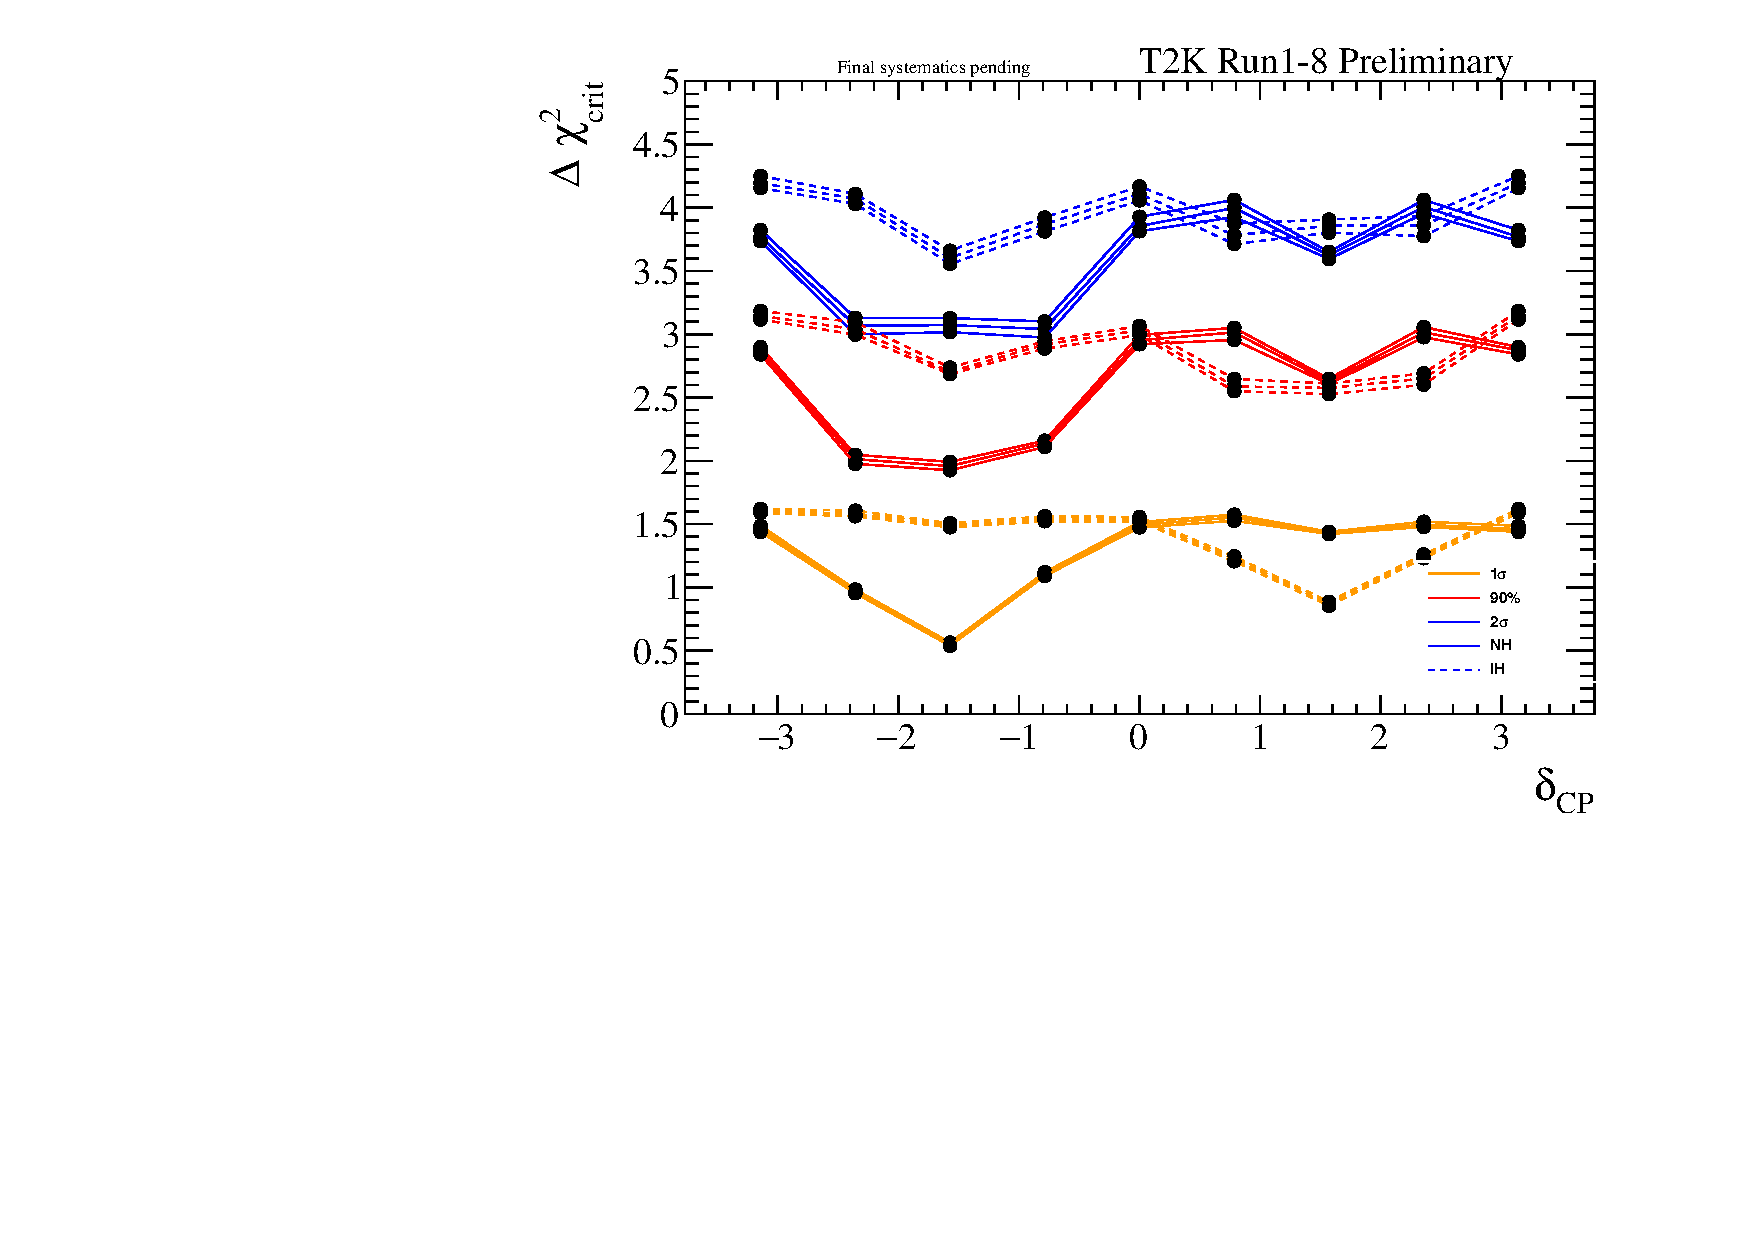
\includegraphics[width=0.9\textwidth]{data/fc/FC_critical_values}
		\caption{\label{fig:fc_critval}Critical $\Delta\chi^2$ values}
	\end{subfigure}
	\begin{subfigure}[b]{0.49\textwidth}
		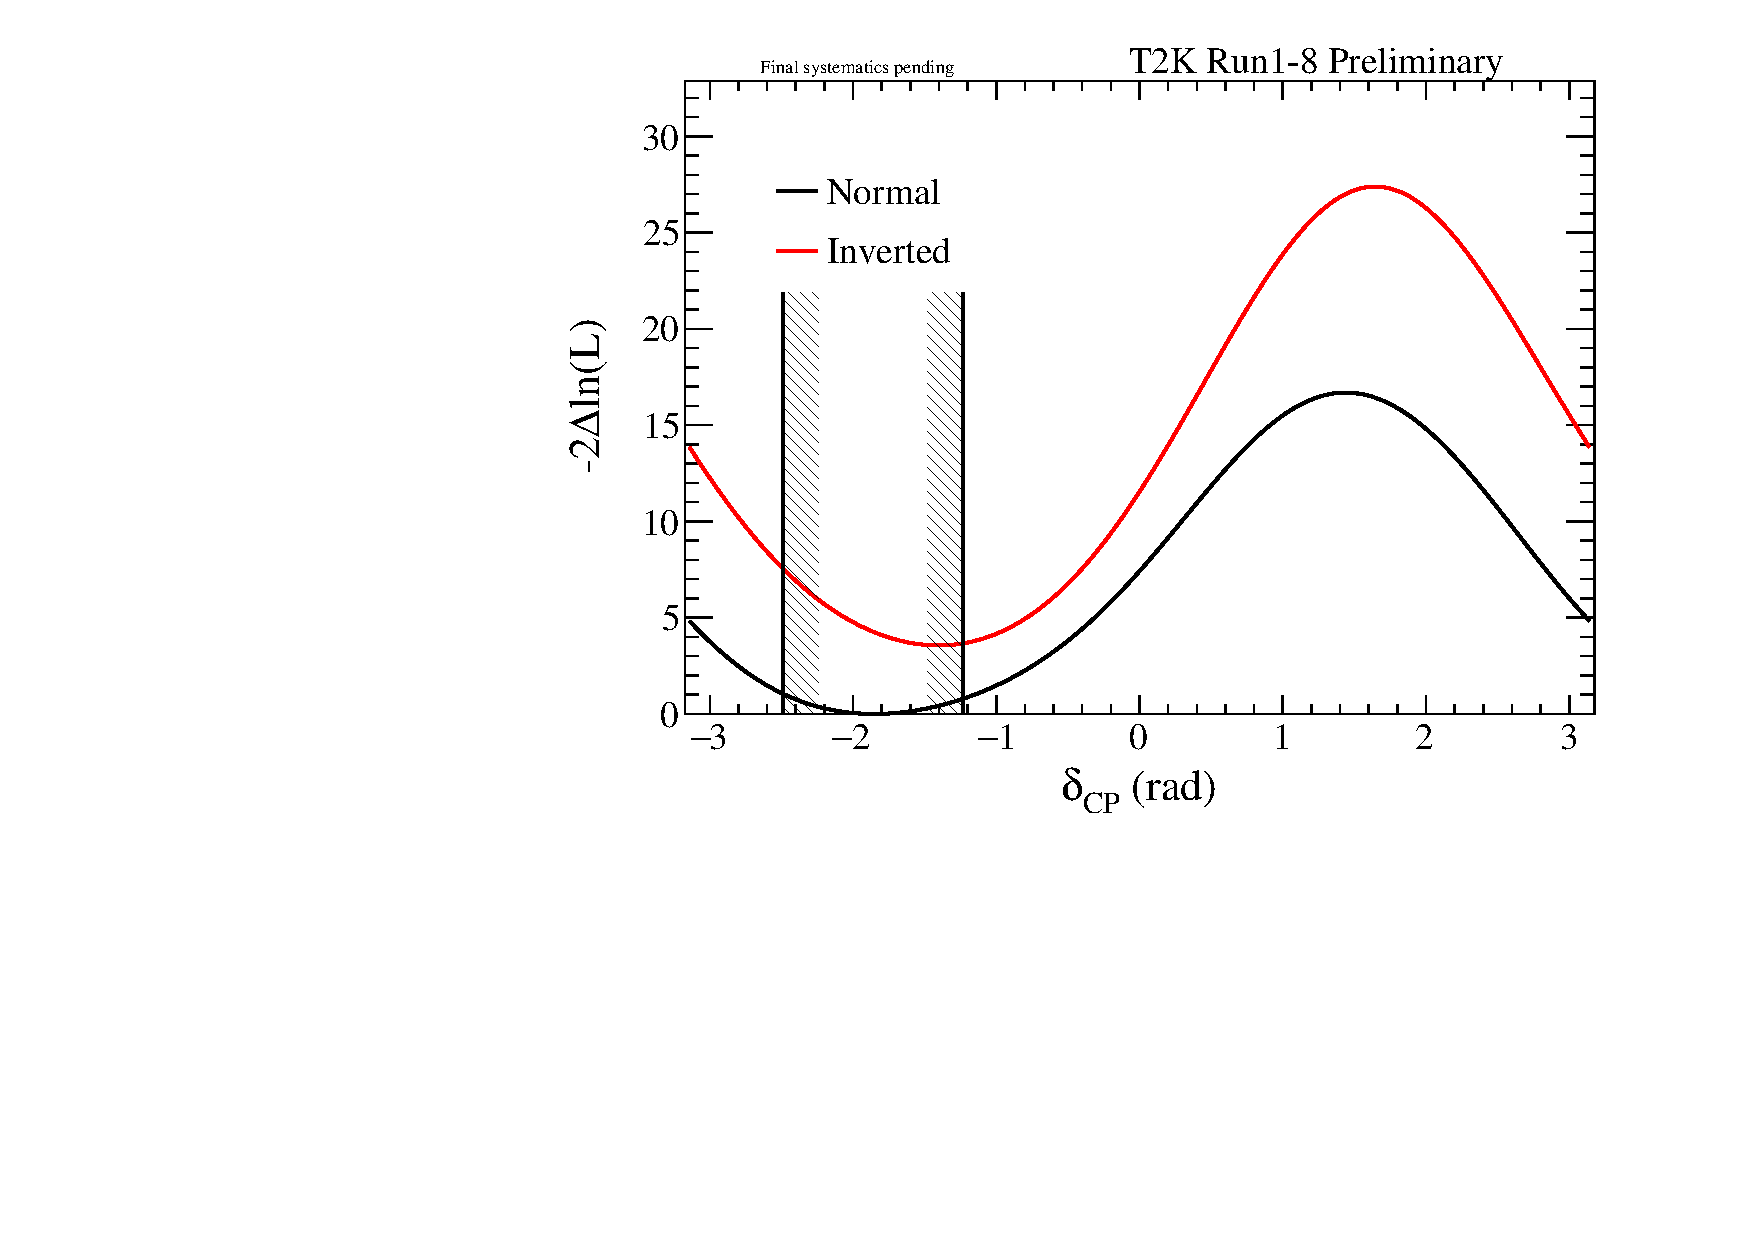
\includegraphics[width=0.9\textwidth]{data/fc/dcp_FC_1sigma_CL}
		\caption{$1\sigma$ CL exclusion region}
	\end{subfigure}
	\begin{subfigure}[b]{0.49\textwidth}
		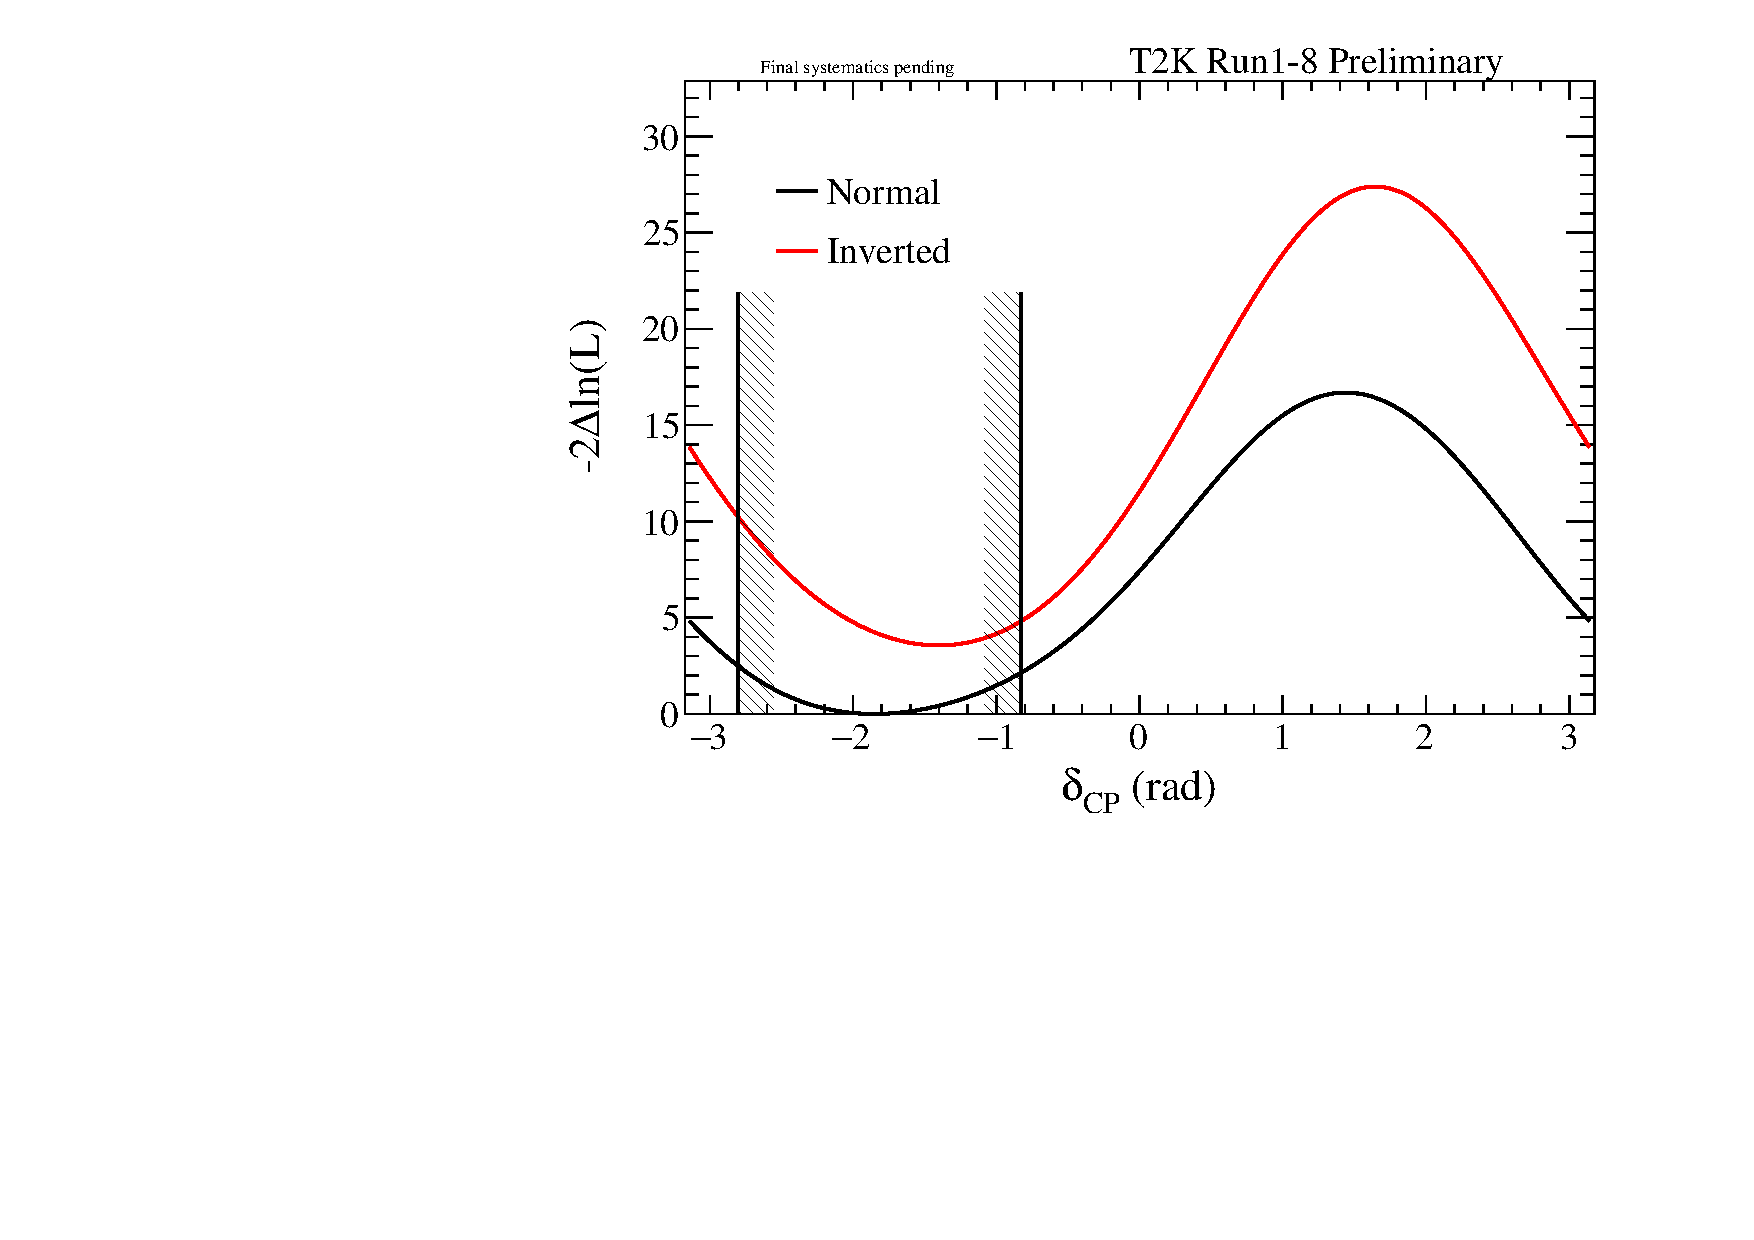
\includegraphics[width=0.9\textwidth]{data/fc/dcp_FC_90_CL}
		\caption{90\% CL exclusion region}
	\end{subfigure}
	\begin{subfigure}[b]{0.49\textwidth}
		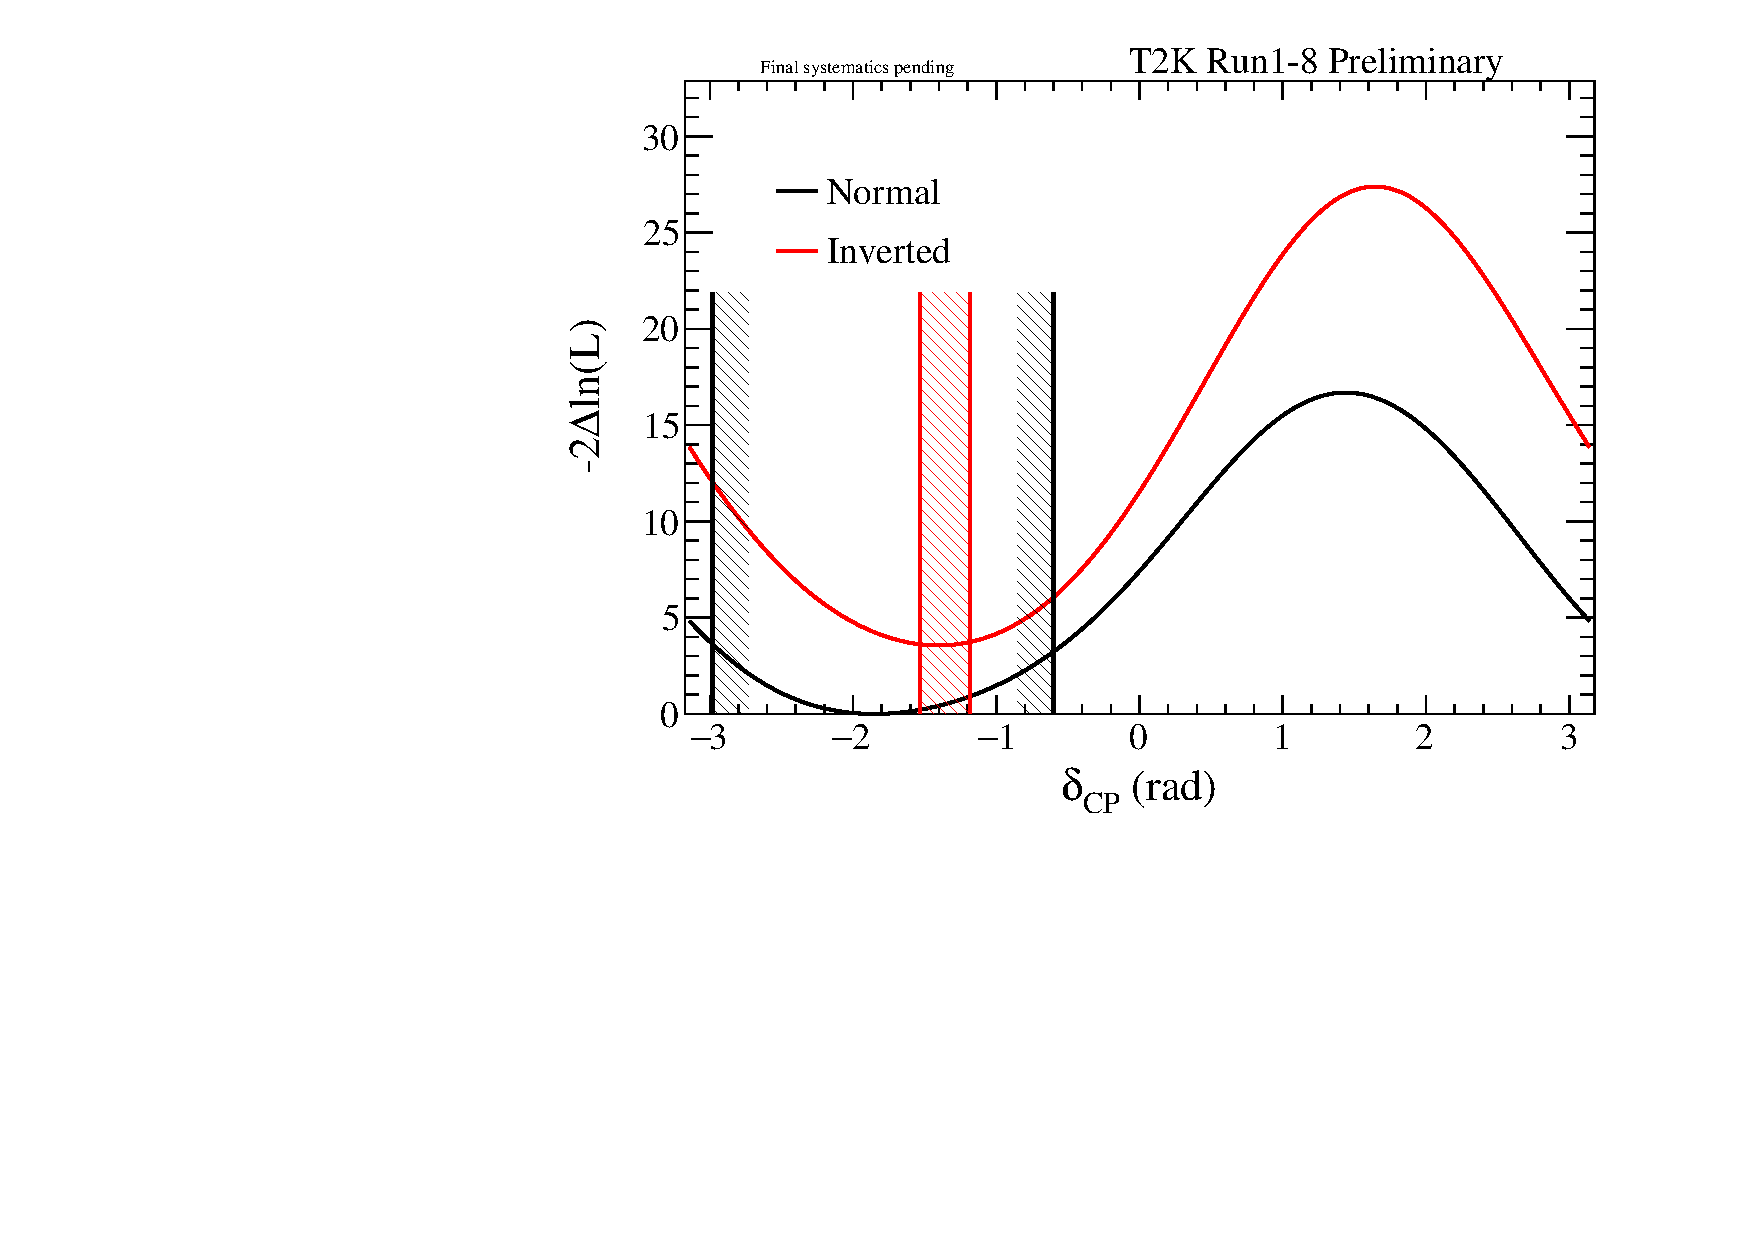
\includegraphics[width=0.9\textwidth]{data/fc/dcp_FC_2sigma_CL}
		\caption{$2\sigma$ CL exclusion region}
	\end{subfigure}
	\caption {
$\Delta\chi^2$ critical values and confidence intervals for the measured $\Delta\chi^2$ distributions for \RunPeriod. Critical values obtained with the Feldman-Cousins method for \RunPeriod for 9 evenly spaced values on the range \( \left[-\pi,\pi\right] \). Critical values are shown for 1\( \sigma \), 2\( \sigma \) and 90\% CL for normal (solid lines) and inverted (dashed lines) hierarchies. At least \num{1e4} toy experiments are performed for each point. The three bands of lines show the \( \pm 1\sigma \) uncertainty on the critical values. Also shown are the measured \( \Delta \chi^2 \) distributions shifted with respect to the same global minium and the $1\sigma$, 90\% and $2\sigma$ exclusion regions for both mass hierarchies. 
	}
	\label{fig:fc_interval}
\end{figure*}

\begin{table}[htb]
	\centering
	\begin{tabular}{| c | c | c | c | c |}
\hline
Parameter & Reactor & CL & Normal hierarchy & Inverted hierarchy \\
\hline
\deltacp		& Yes & 90\% & $\left[ -2.805, -0.830 \right]$ & - \\
\deltacp		& Yes & $ 2\sigma $ & $\left[ -2.981, -0.600 \right]$ & $\left[ -1.531, -1.184 \right]$ \\
\hline
\end{tabular}

	\caption{
		The confidence intervals at 90\% CL and $2\sigma$ CL obtained with the Feldman-Cousins method for the \RunPeriod data set is shown for the measurement of \deltacp versus mass hierarchy.
	}
	\label{tab:fc_interval}
\end{table}

%
%
%In \cref{fig:joint_dcp_fc_run17c} the confidence intervals obtained with the ``Feldman-Cousins" method
%are shown for $\delta_{CP}$ and mass hierarchy with reactor constraint for the Run 1-7c data set.
%The critical values at both 90\% and $2\sigma$ CL are computed
%for both the mass hierarchies and the following true values of $\delta_{CP}$: 
%$-\pi$, -2.356, $-\pi/2$, -0.785, 0, +0.785, $+\pi/2$, -2.356, $+\pi$. 
%The procedure described in \cref{sec:cl} is used.
%About 10k toy experiments were used for all the true points except $\delta_{CP} = \pi$ - normal hierarchy.
%Indeed the Run 1-7c data $\Delta \chi^2$ value is very close to the 90\% CL critical value, within one standard deviation of the critical value,
%if only 10k toy experiments are used. 
%For this reason, in order to provide a more precise statement about the 
%90\% CL exclusion of $\delta_{CP} = \pi$ - normal hierarchy, about 28k toy experiments are used, 
%so that the data $\Delta \chi^2$ value is outside the $\pm 1 \sigma$ critical value error.
%This can be seen in in \cref{fig:joint_dcp_fc_run17c}
%where the $\pm 1 \sigma$ error on the critical values are shown as well.
%The same procedure used for the Run 1-6 and Run 1-7b data fit, shown in \cref{sec:fc_significance}, is used.
%Inverted hierarchy is almost excluded at 90\% CL except for a small interval around $\delta_{CP} = -\pi / 2$.
%$\delta_{CP} = 0$ is still disfavored with respect to $\delta_{CP} = \pi$, which, however, is excluded at 90\% CL. 
%We can say that CP conservation assuming the PMNS framework is excluded at 90\% CL also for the Run 1-7c data set,
%though the p-value for $\delta_{CP} = \pi$ and normal hierarchy is very close to 0.1. 
%
%\begin{figure*}[htb]
%\center
%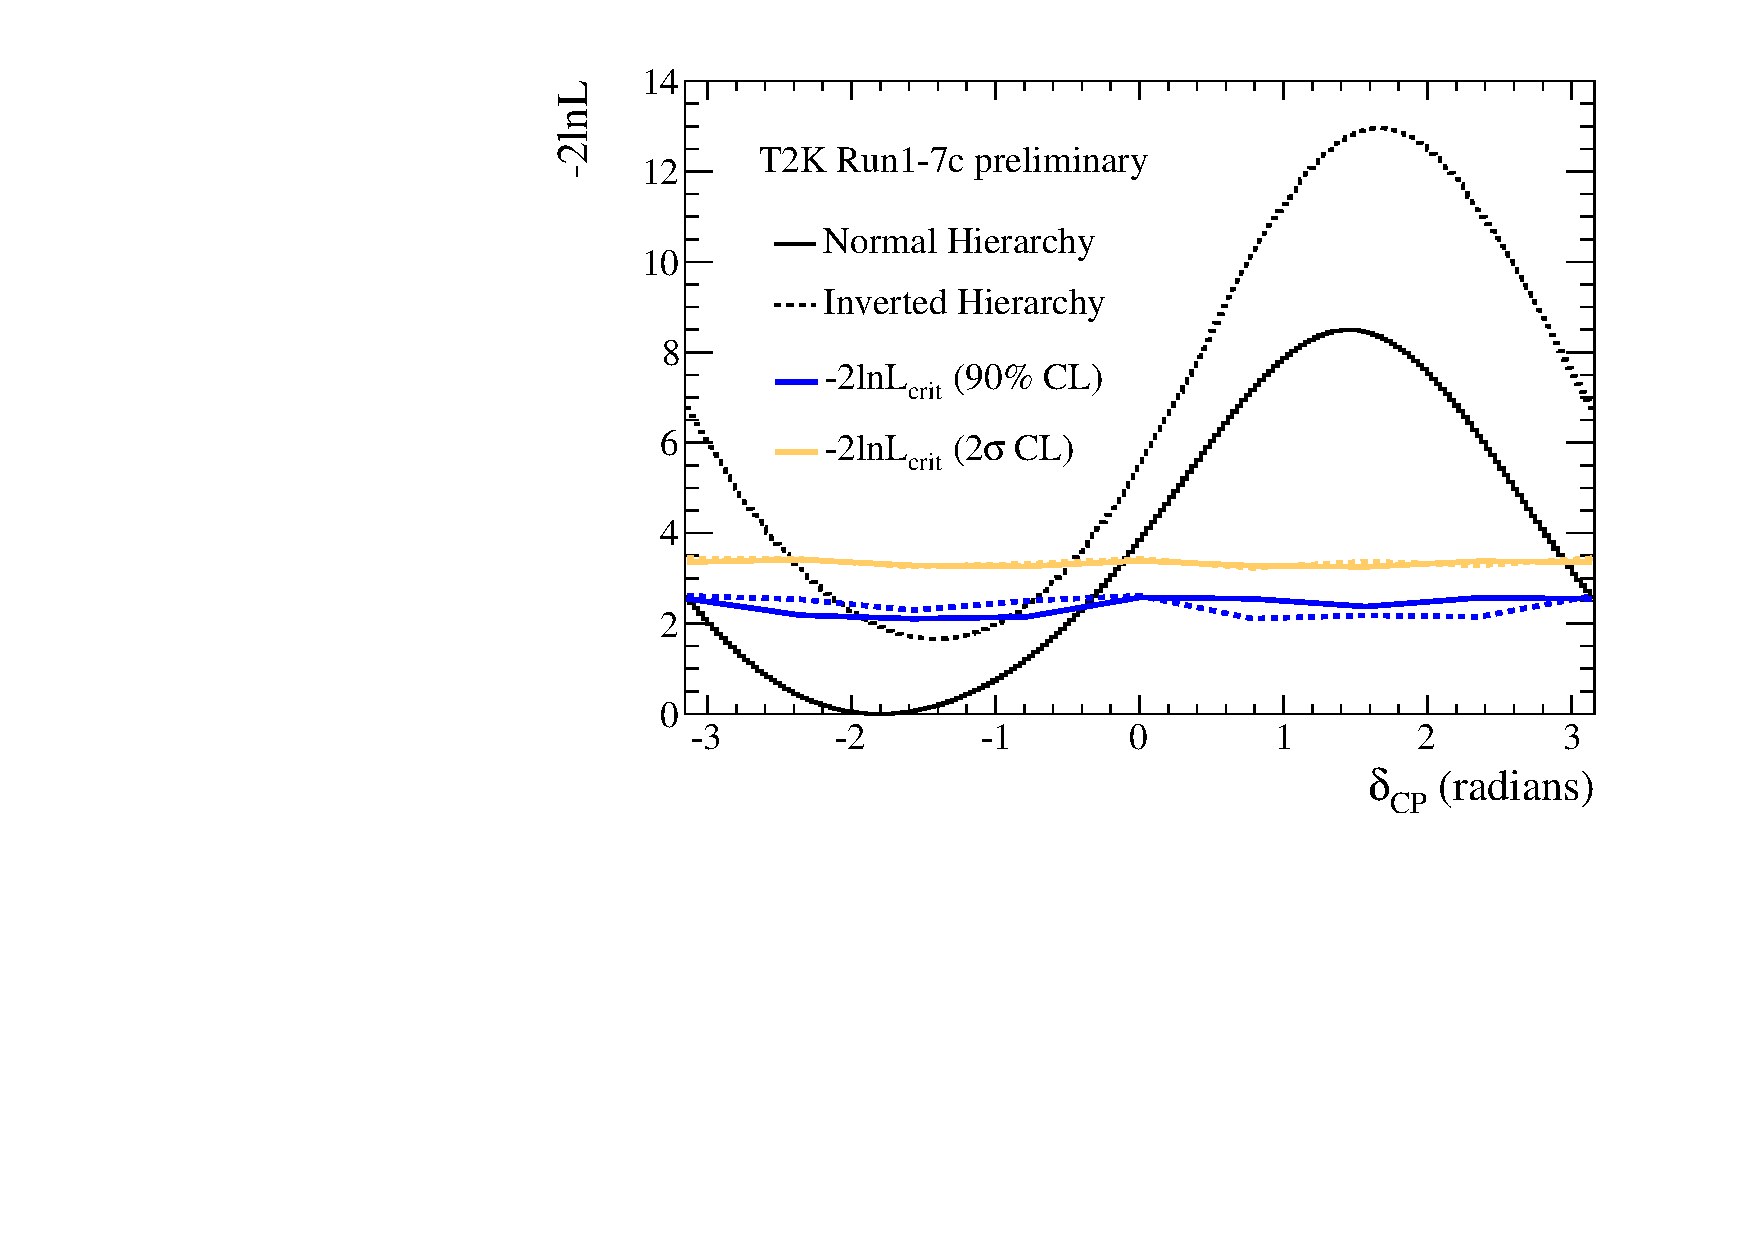
\includegraphics[width=0.49\textwidth]{joint_plots/coverage_fc/fc_run17c/dcp_mh_react_run17.pdf} 
%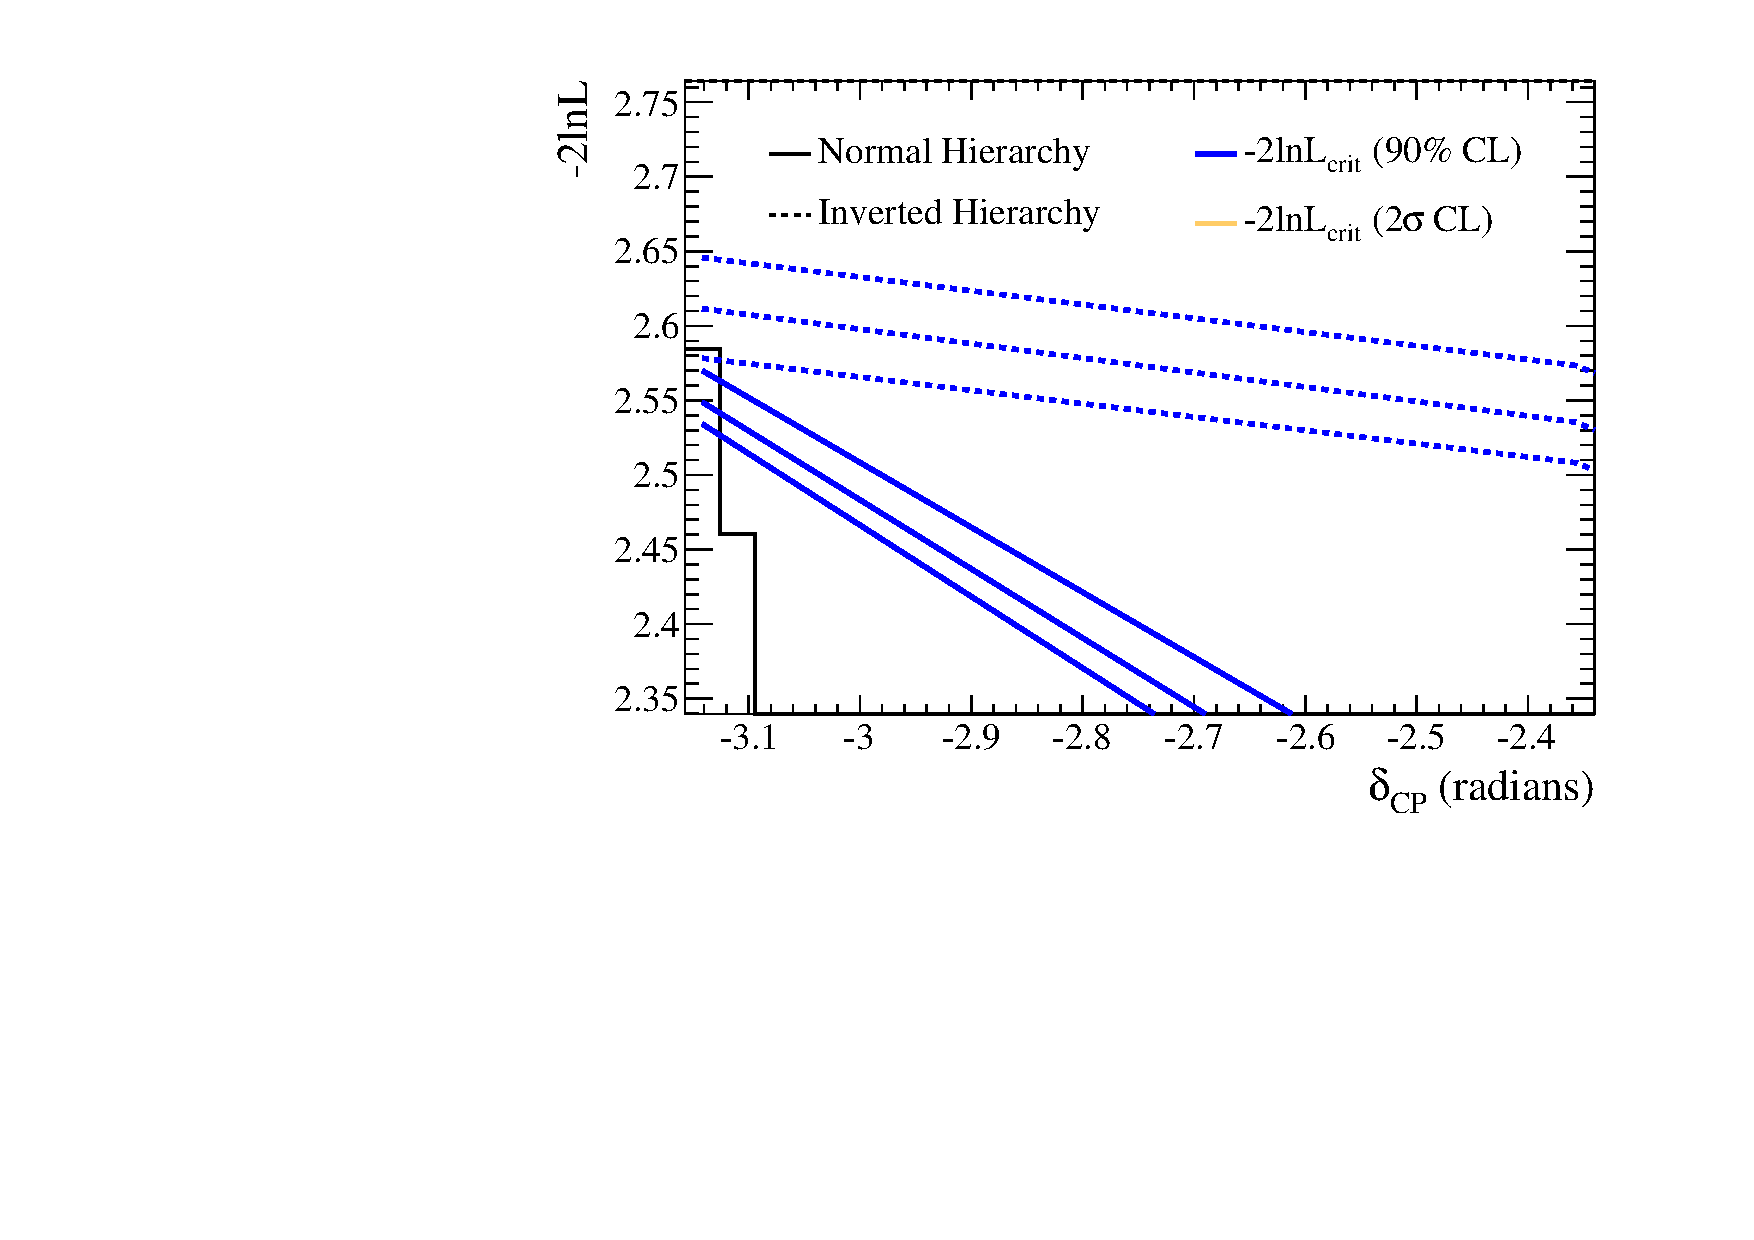
\includegraphics[width=0.49\textwidth]{joint_plots/coverage_fc/fc_run17c/dcp_mh_react_run17_zoom.pdf} \\
%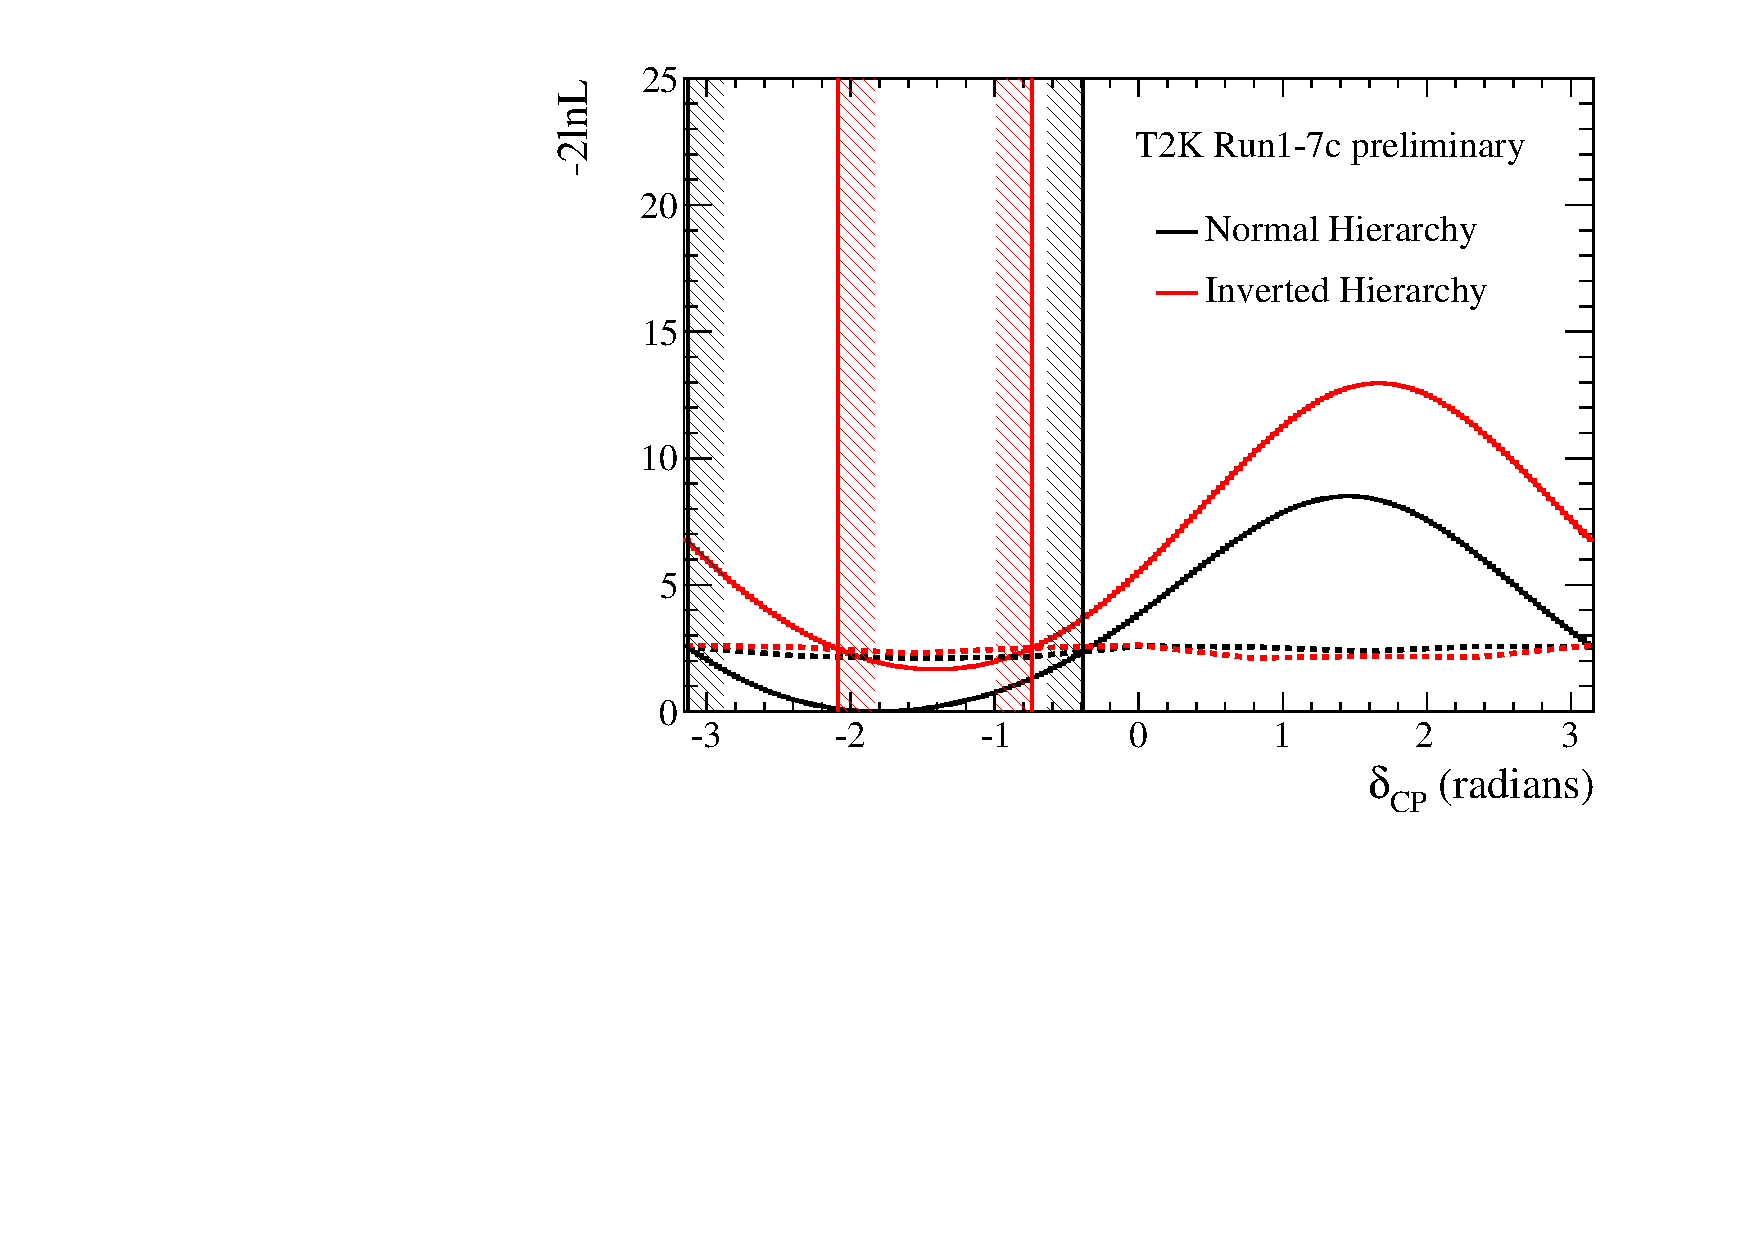
\includegraphics[width=0.49\textwidth]{joint_plots/coverage_fc/fc_run17c/dcp_mh_react_run17_interval_90CL.pdf} 
%\caption{
%Measured $\Delta \chi^2$ distributions with the full Run 1-7c data set.
%Both normal (black solid line) and inverted (black dashed line) hierarchies are shown. 
%The ``Feldman-Cousins" method is used to set the $\Delta \chi^2$ critical values in order to provide 
%confidence intervals with the proper coverage.
%The ranges of $\delta_{CP}$ which correspond to $\Delta \chi^2$ values larger than the critical 
%values (blue for 90\% CL and orange for $2\sigma$ CL) are excluded at a certain confidence level.
%Both normal and inverted hierarchy $\Delta \chi^2$ distributions are shifted with respect to the same global minimum. 
%All the oscillation parameters which are not parameters of interest
%are marginalised using the prior distributions shown in \cref{tab:marg_binnning}.
%The $\pm1 \sigma$ error on the critical values is shown as well, where specified, 
%and is represented by the lowest and highest set of critical values, with the same colour of the central ones.
%On the right plot a zoom on the critical values is shown.
%}
%\label{fig:joint_dcp_fc_run17c}
%\end{figure*}
%
%
%
%In \cref{tab:joint_bestfit_dcp_90CL_interval_FC_run17c} the 90\% CL intervals for $\delta_{CP}$ vs mass hierarchy,
%obtained with the Feldman-Cousins method, are shown.
%
%
%% Interval of deltaCP for 90% CL w/ Feldman-Cousins
%
%\begin{table}[htb]
%\centering
%\begin{tabular}{| c | c | c | c |}
%\hline
%{\bf Parameter}						& {\bf Reactors}		& {\bf Normal Hierarchy}		& {\bf Inverted Hierarchy}		\\
%\hline
%$\delta_{CP}$ (radians) 				& YES      			& [-3.13; -0.39]				& [-2.09; -0.74]				\\
%\hline
%\end{tabular}
%\caption{
%The confidence intervals at 90\% CL obtained with the Feldman-Cousins method
%for the Run 1-7c data set
%is shown for the measurement of $\delta_{CP}$ vs mass hierarchy.
%The reactor constraint $\sin^2 2\theta_{13} = 0.085 \pm 0.005 $ \cite{pdg_2014} is applied.
%}                                                                                                                                                                                          
%\label{tab:joint_bestfit_dcp_90CL_interval_FC_run17c}
%\end{table}
%
%
%\clearpage

\subsection {Discussion of the \RunPeriod data fit results}
\label{sec:results:discussion}

The \nueCConepi data set shows an excess in the number of observed appearance events, observing 15 events compared to an Asimov A expectation of 7. Unlike in our previous analysis, an excess is not observed in the neutrino mode one ring $e$-like sample, rather in this analysis we see a deficit in the number of observed events in neutrino mode one ring $\mu$-like sample, observing 240 against an Asimov A expectation of 268.

The value of \deltacp favoured by the joint fit analysis, when the reactor constraint is applied, is \BestFitDeltacpwRC and corresponds to normal hierarchy. If the reactor constraint is not applied, the best-fit value of \deltacp is \BestFitDeltacpwoRC and $\delta_{CP}=0$ is still excluded at $2\sigma$ CL.

When considering the constant $\Delta\chi^2$ method, we see that the constraint on \deltacp is stronger than expected. To investigate the source of this difference a number of fits were undertaken using hybrids of data and MC. In particular \cref{fig:deltacp_hybrids} shows the expected sensitivity from the Asimov A data set (dashed), the data fit (solid black) and then a number of additional fits where one of the data samples was replaced by the corresponding Asimov A sample (e.g. Data x1Rmu indicates a fit of 4 data samples, with the one-ring $\mu$-like sample being replaced by the Asimov A prediction). From this one can see that the largest contribution to the stronger constraint comes from the upward fluctuation observed in the \nueCConepi{} sample, but contributions are also evident from the FHC one-ring $\mu$-like sample, where a deficit in events is seen, and from the two one-ring $e$-like samples. This results in the exclusion of CP-conservation at more than $2 \sigma$ with the reactor constraint applied and the inverted hierarchy is disfavoured at 90\%CL. The effect is also apparent in the appearance contour.

\begin{figure*}[htb]
	\center
	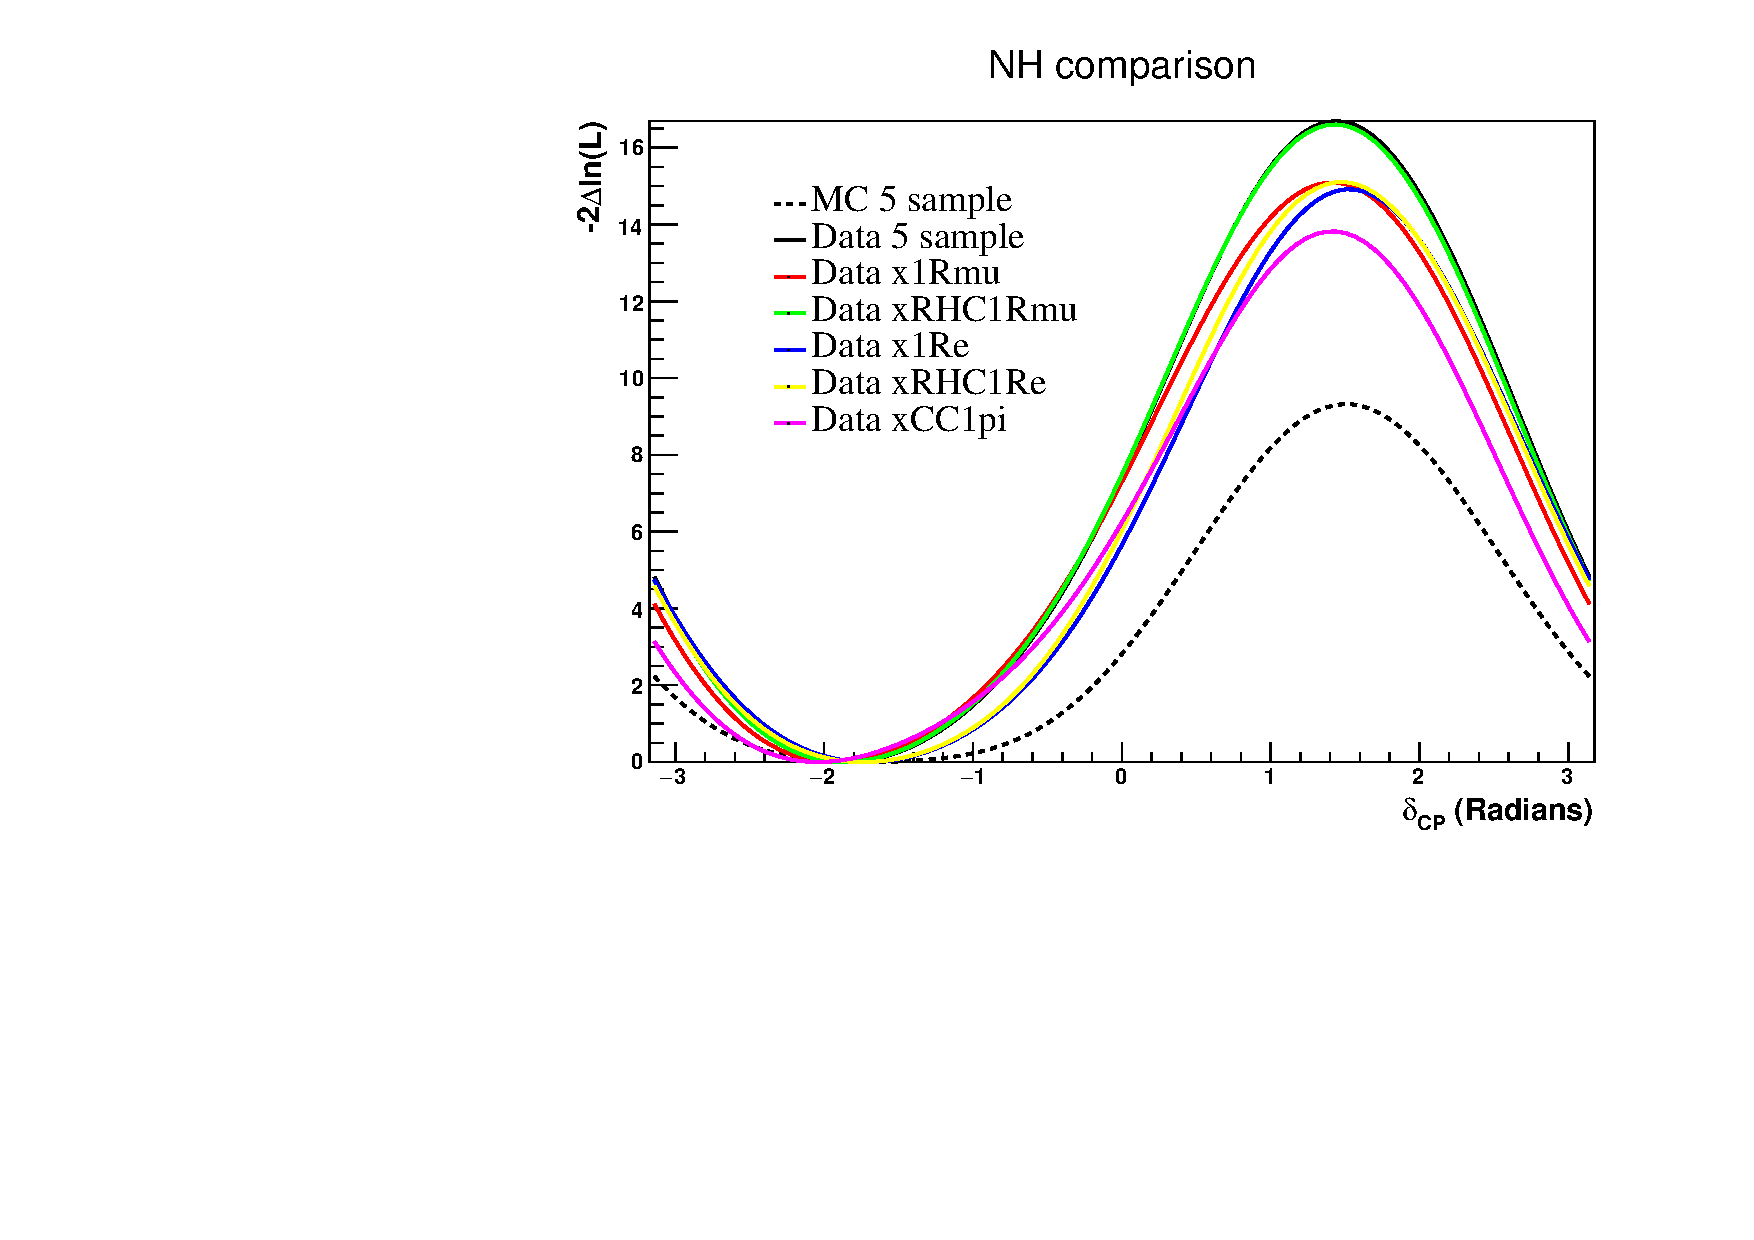
\includegraphics[width=0.9\textwidth]{studies/hybrids/deltacp_hybrids}
	\caption {
		The expected $\Delta\chi^2$ distribution as a function of \deltacp with reactor constraint for MC, data and data/MC hybrid data sets.
	}
	\label{fig:deltacp_hybrids}
\end{figure*}

% <THIS MAY BE RELEVANT COMPARING 4 SAMPLE TO 5 SAMPLE IF THE 5 SAMPLE PREFERS A LARGER THETA13 THAN THE 4 SAMPLE> The effect is also apparent in the $\sin^2 \theta_{13}$ Vs $\delta_{CP}$ contours where the new analysis prefers a larger value of $\sin^2 \theta_{13}$ which, when constrained by the reactor measurements, results in a stronger constraint on $\delta_{CP}$. 


% <AS ABOVE> The comparison of the fits to $\sin^2 \theta_{23}$ Vs $\Delta m^2_{32}$ are slightly unexpected considering the sensitivity study, however the result where a greater portion of the lower octant of $\sin^2 \theta_{23}$ is excluded at 90\%CL and 68\%CL can be explained again by the excess of events observed in the \nueCConepi{}  which favour a much larger value of $\sin^2 \theta_{23}$ and therefore push the parameter to the upper octant. \color{red}(speculative, needs confirmation)\color{black}

A stronger than expected constraint is also evident in the disappearance contour, with greater exclusion in \ssqthtwothree. Similarly to the \deltacp hybrid fits above, \cref{fig:disappearance_hybrids} shows the expected sensitivity from the Asimov A data set (red), the data fit (black) and then a number of additional fits where one of the data samples was replaced by the corresponding Asimov A sample. From this one can see that the stronger constraint can be explained by the deficit in the observed number of events in the one-ring $\mu$-like sample.

\begin{figure*}[htb]
	\center
	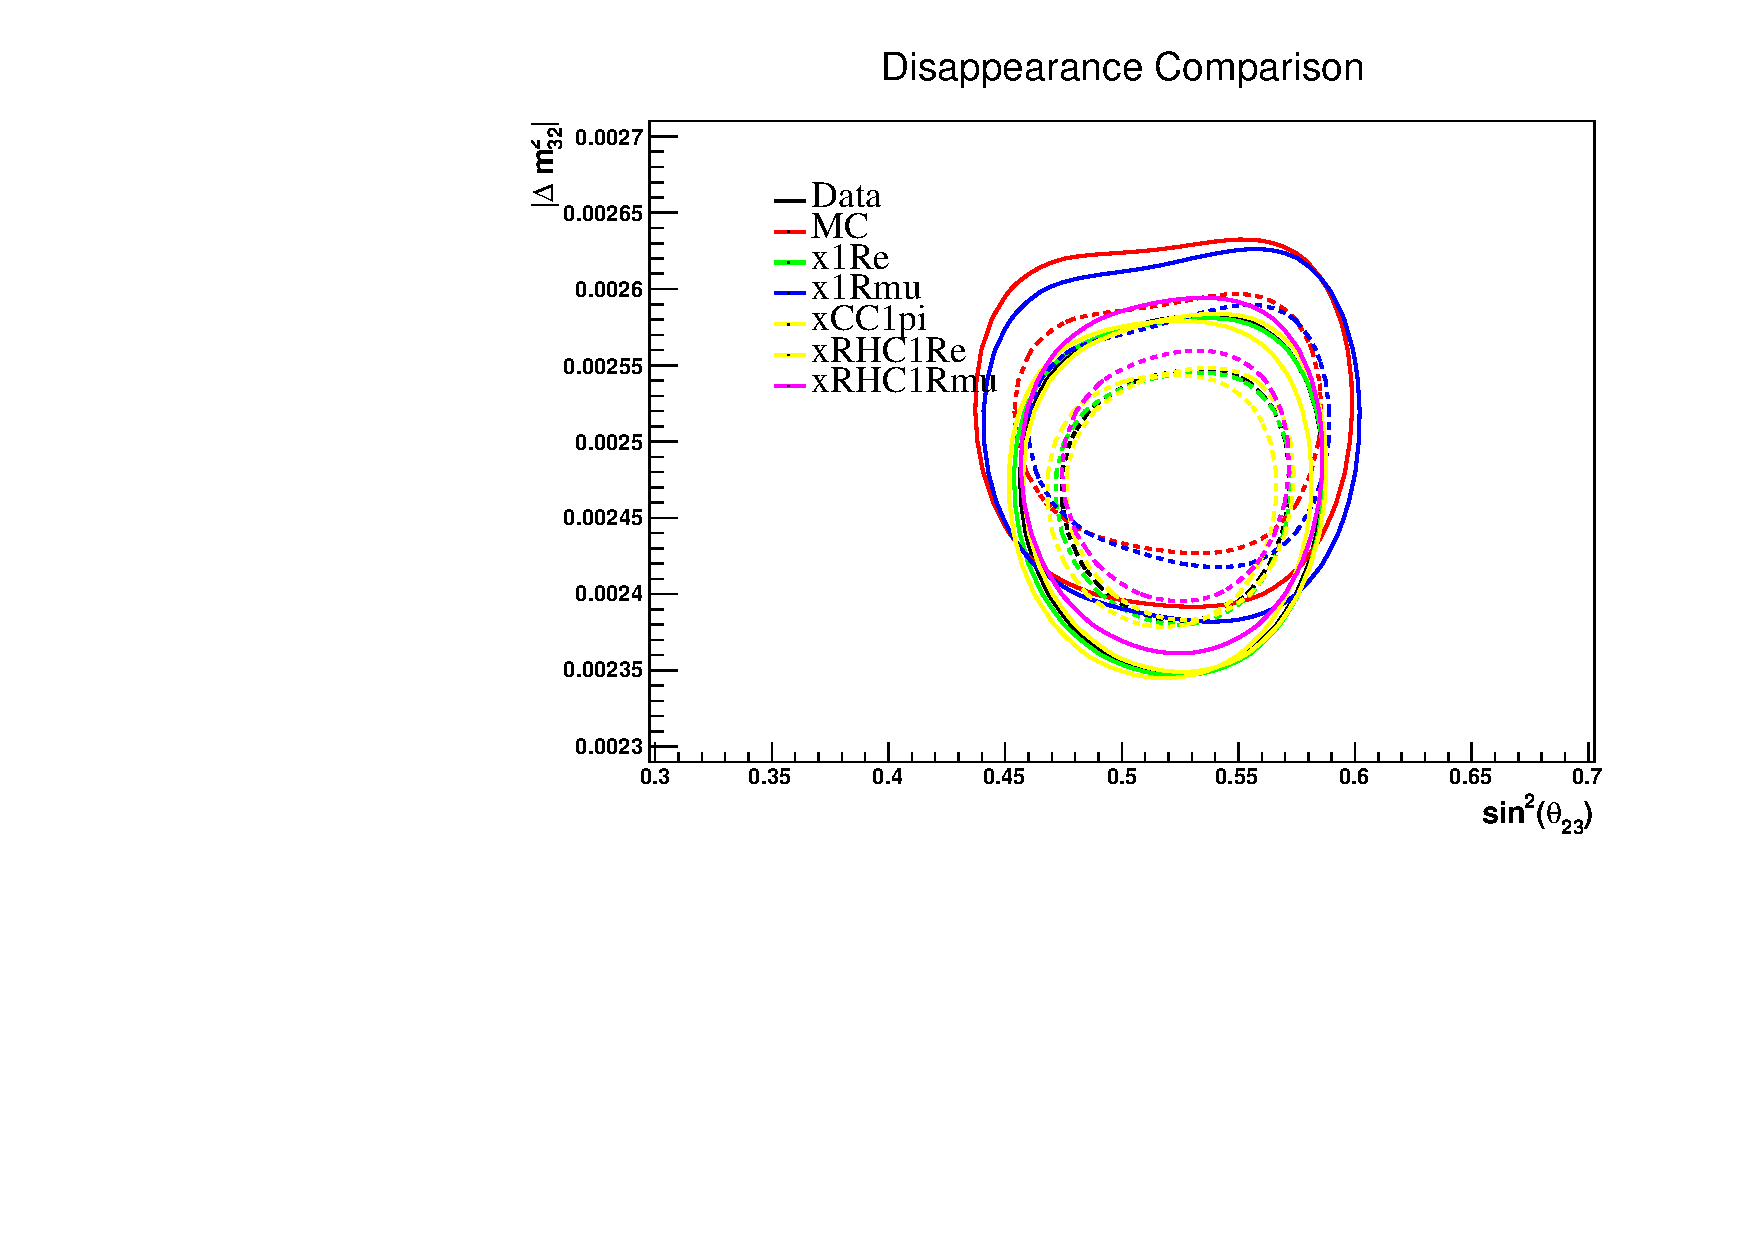
\includegraphics[width=0.9\textwidth]{studies/hybrids/disappearance_hybrids}
	\caption {
		The expected disappearance contours with reactor constraint for normal hierarchy for MC, data and data/MC hybrid data sets.
	}
	\label{fig:disappearance_hybrids}
\end{figure*}

% <AS ABOVE> The comparison of the fits to $\sin^2 \theta_{23}$ Vs $\Delta m^2_{32}$ are slightly unexpected considering the sensitivity study, however the result where a greater portion of the lower octant of $\sin^2 \theta_{23}$ is excluded at 90\%CL and 68\%CL can be explained again by the excess of events observed in the \nueCConepi{}  which favour a much larger value of $\sin^2 \theta_{23}$ and therefore push the parameter to the upper octant. \color{red}(speculative, needs confirmation)\color{black}

The value of \ssqthonethree favoured by the analysis is \BestFitMixingOneThreewoRC and corresponds to normal hierarchy, with the 1D contours in agreement with the PDG 2016 reactor constraint ($0.0219 \pm 0.0012$) at $\sim1.2 \sigma$ (see \cref{tab:data_bestfit}).

The value of \ssqthtwothree favoured by the analysis is \BestFitMixingTwoThreewRC (\BestFitMixingTwoThreewoRC) with (without) the reactor constraint and corresponds to normal hierarchy, with the 1D contours in agreement with and without the reactor constraint at $1 \sigma$, favouring maximal mixing as seen in our previous analyses.

The value of \dmsqtwothree favoured by the analysis is \BestFitDmTwoThreewRC $\times 10^{-3}\text{ eV}^2\text{/c}^4$ (\BestFitDmTwoThreewoRC$\times 10^{-3}\text{ eV}^2\text{/c}^4$) with (without) the reactor constraint and corresponds to normal hierarchy, with the 1D contours in agreement with and without the reactor constraint at $1 \sigma$.

\subsection {Comparison of \deltacp versus mass hierarchy result with sensitivity}
\label{sec:results:brazilian}

In order to provide a better understanding of the results of the \RunPeriod data fit, the result has been compared with the expected sensitivity obtained from a large number (10k) of toy experiments for different true value of \deltacp (currently only $\delta_{CP} = -\pi/2$ is included) and the mass hierarchy.

\subsubsection{Expected sensitivity method}
\label{sec:results:brazilian:method}
This section outlines the procedure to produce the expected sensitivity comparison plots. The example given is for true normal hierarchy and $\delta_{CP} = -\pi/2$.
\begin{itemize}
	\item \num{1e4} fake data sets are generated following the Feldman-Cousins method for a true value of \deltacp and mass hierarchy, in this case $\delta_{CP} = -\pi/2$ and normal hierarchy.
	\item A $\chi^2$ distribution is computed with respect to the marginalisation toys as a function of \deltacp and mass hierarchy.
	\item For each fake data set, the minimum value of $\chi^2$ for each bin of \deltacp, $\chi^2_{bin,min}$ is found with respect to both normal and inverted hierarchy.
	\item The test statistic is then computed as $\Delta\chi^2_{bin} = \chi^2_{bin} - \chi^2_{bin,min}$, which is slightly different to the Feldman-Cousins method, where $\Delta\chi^2_{FC} = \chi^2_{true} - \chi^2_{best-fit}$. The distributions of $\Delta\chi^2_{bin}$ and $\Delta\chi^2_{FC}$ coincide if the bin is $\delta_{CP} = -\pi/2$ and normal hierarchy, i.e. the true point used to generate the toy experiments.
	\item This results in a $\Delta\chi^2$ distribution from which we can draw conclusions about the expected $\Delta\chi^2$ for each value of \deltacp given a hypothesised true value and hierarchy.
	\item The spread of the $\Delta\chi^2$ distribution for each point of \deltacp and mass hierarchy is obtained as the range of the $\Delta\chi^2_{bin}$ distribution that contains respectively the 68.27\% and 95.45\% of the toy experiments on its left side. The test statistic $\Delta\chi^2_{bin}$ is assumed ot be 1-sided because by construction $\chi^2_{bin,min} \le \chi^2_{bin}$.
	\item An alternative to the one-sided distribution is also produced, for which values of $\Delta\chi^2$ of each bin of \deltacp are themselves binned (100 evenly-spaced bins on the range [$\Delta\chi^2_{bin,min},\Delta\chi^2_{bin,max}$]) and then toys are added to the expected sensitivity bands starting from the bin of $\Delta\chi^2$ that contains the most toys, until 68.27\% and 95.45\% of the toy experiments have been included, thereby producing two-sided distributions.
	\item A plot is also produced to show the fraction of toy experiments which exclude each value of \deltacp to greater than $2\sigma$ significance in the Feldman-Cousins corrected critical values along with the probabilities to exclude $\delta_{CP} = 0$ and $\delta_{CP} = \pi$ for a given true value of \deltacp.
\end{itemize}

\subsubsection{$\delta_{CP} = -\pi/2$ - normal hierarchy}

In \cref{fig:brazilian_dcp_mpi2} the \RunPeriod data result for \deltacp versus mass hierarchy is compared to the $1\sigma$ and $2\sigma$ uncertainties on the $\Delta\chi^2$ distributions corresponding to $\delta_{CP} = -\pi/2$ and (a) normal hierarchy and (b) inverted hierarchy. We see that the data contour is contained within the $2\sigma$ band for inverted hierarchy, whilst the data contour falls just outside the $2\sigma$ band for normal hierarchy in the region around $\delta_{CP} = 0$. This suggests that the data constraint is consistent with the PMNS matrix at around the $2\sigma$ level.

We also see an interesting feature near $\delta_{CP} = -\pi/2$ where the $\Delta\chi^2$ values have a wider distribution. This is due to the boundary at $\delta_{CP} = -\pi/2$ which causes a wider distribution when the parameter \deltacp would like to be pushed beyond the boundary in the fit.

Finally from \cref{fig:brazilian_dcp_mpi2}(c) we see that $\delta_{CP} = 0$ and $\delta_{CP} = \pi$ are excluded at 90\% confidence level in around 40\% (see \cref{tab:exclusion_prob}) of the toy experiments and excluded at $2\sigma$ confidence level in between 25\% and 30\% of the toy experiments, with $\delta_{CP} = \pi$ excluded in slightly fewer toy experiments in each case.

\begin{figure*}[htb]
	\center
	\begin{subfigure}[b]{0.49\textwidth}
		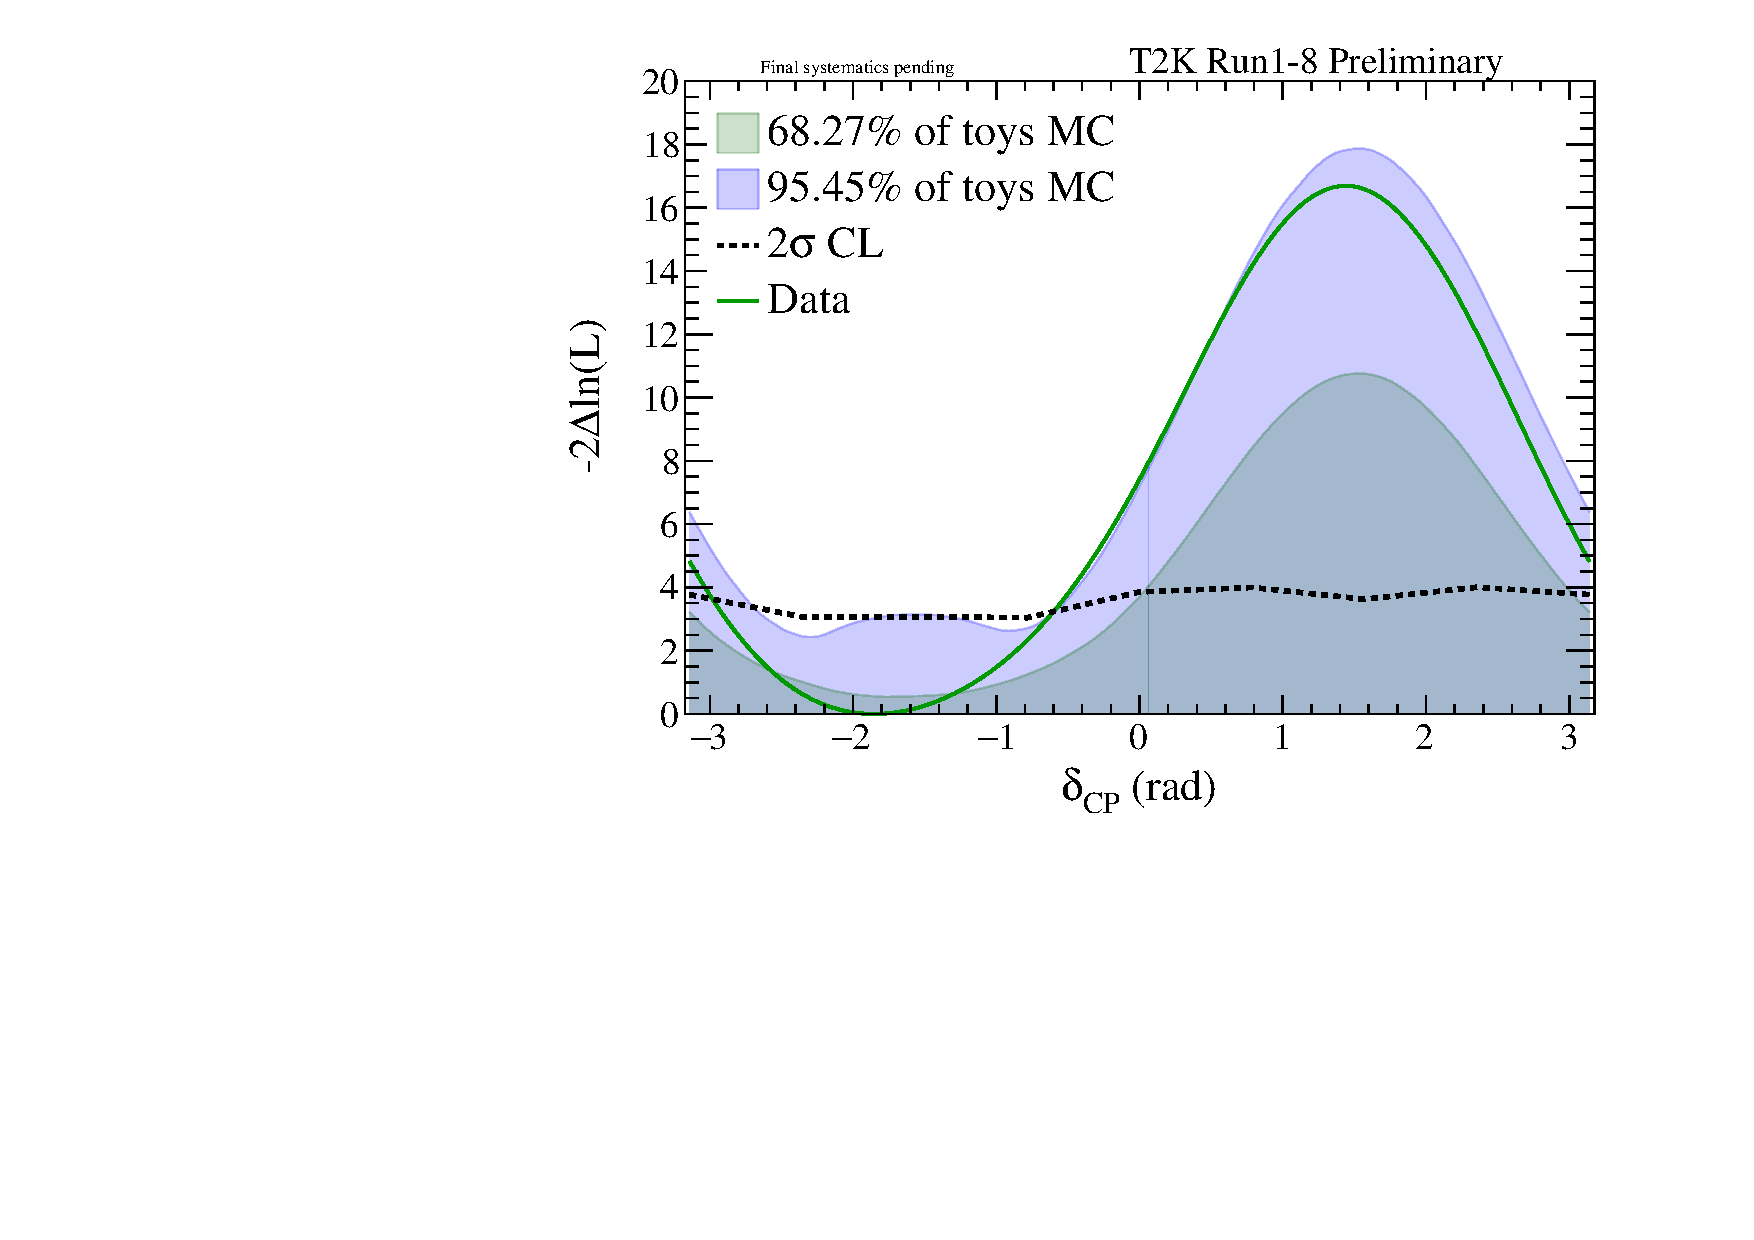
\includegraphics[width=0.9\textwidth]{comparison/dcp_run18_react_Data_braz_nh}
		\caption{Normal hierarchy}
	\end{subfigure}
	\begin{subfigure}[b]{0.49\textwidth}
		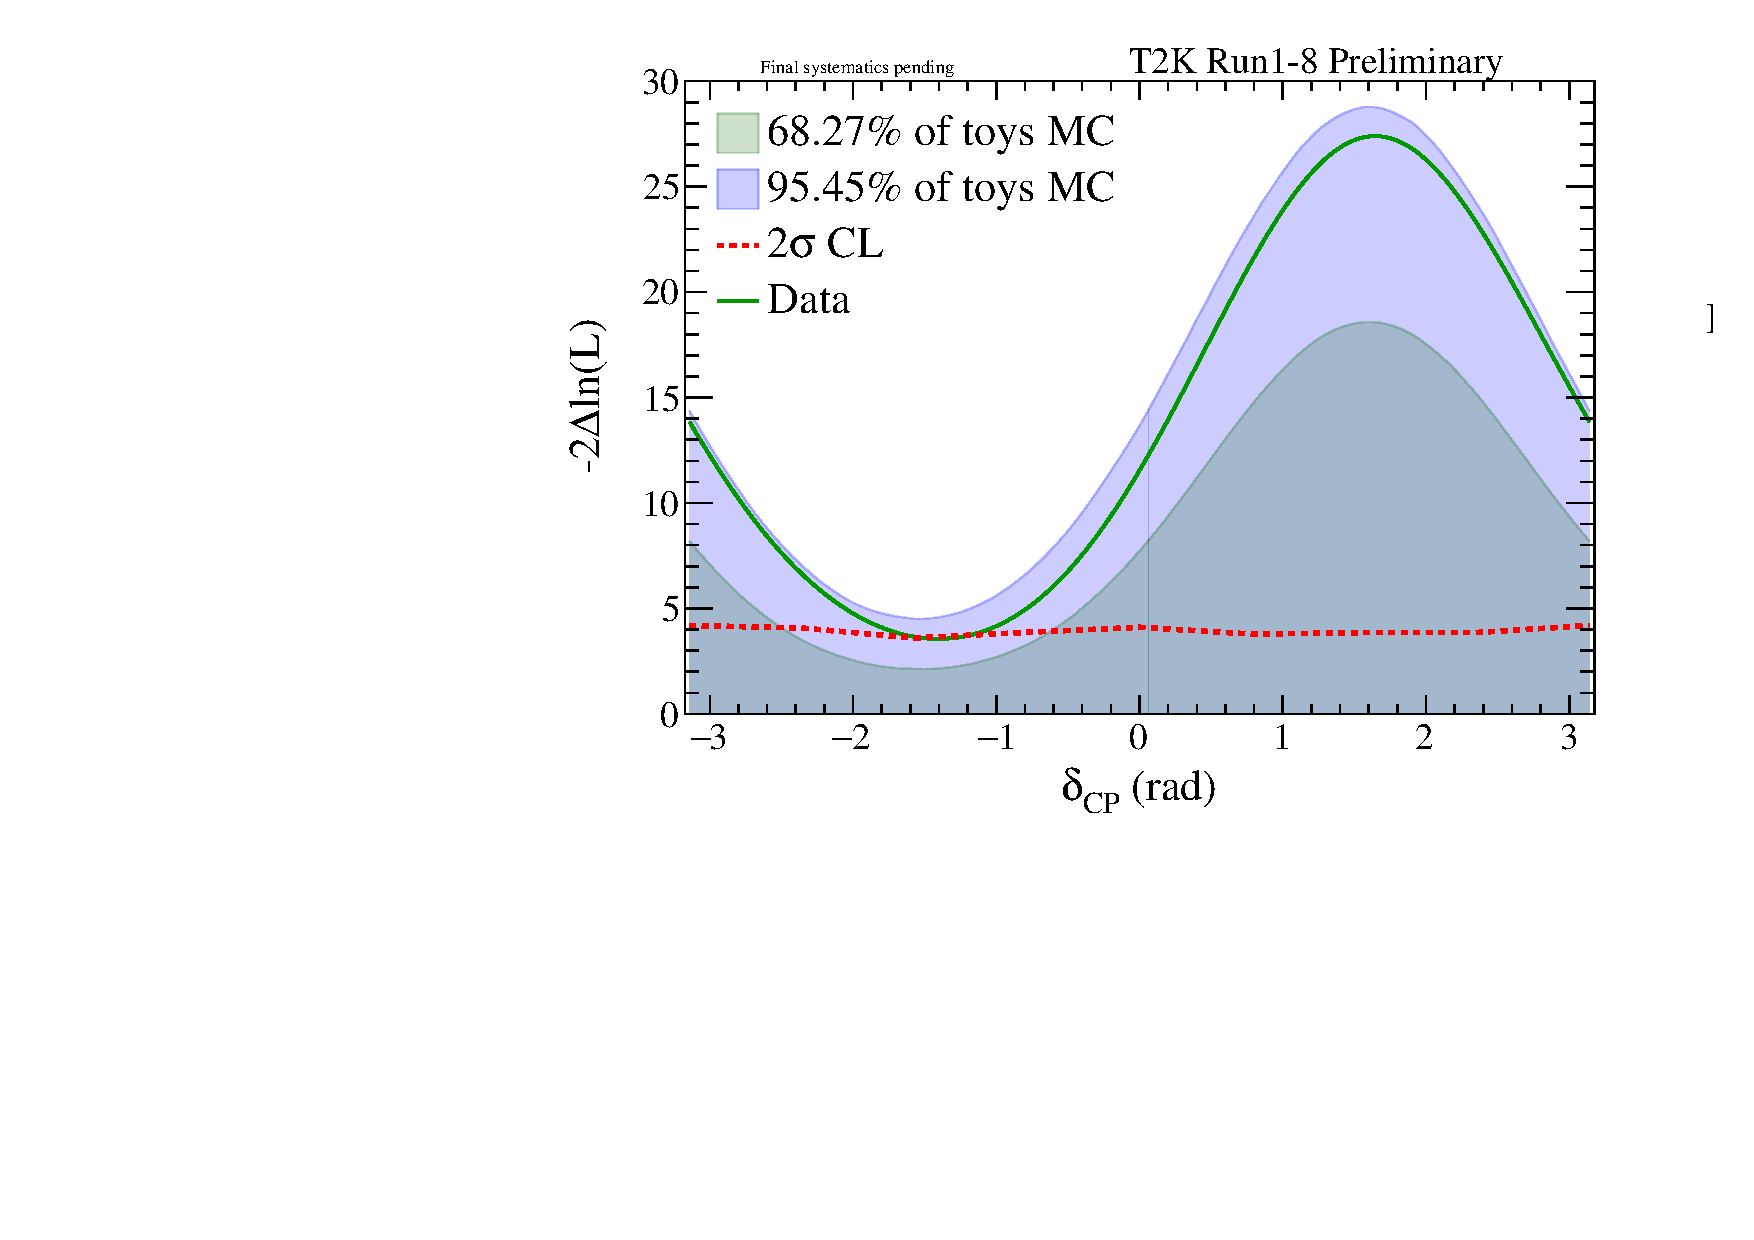
\includegraphics[width=0.9\textwidth]{comparison/dcp_run18_react_Data_braz_ih}
		\caption{Inverted hierarchy}
	\end{subfigure}
	\begin{subfigure}[b]{0.49\textwidth}
		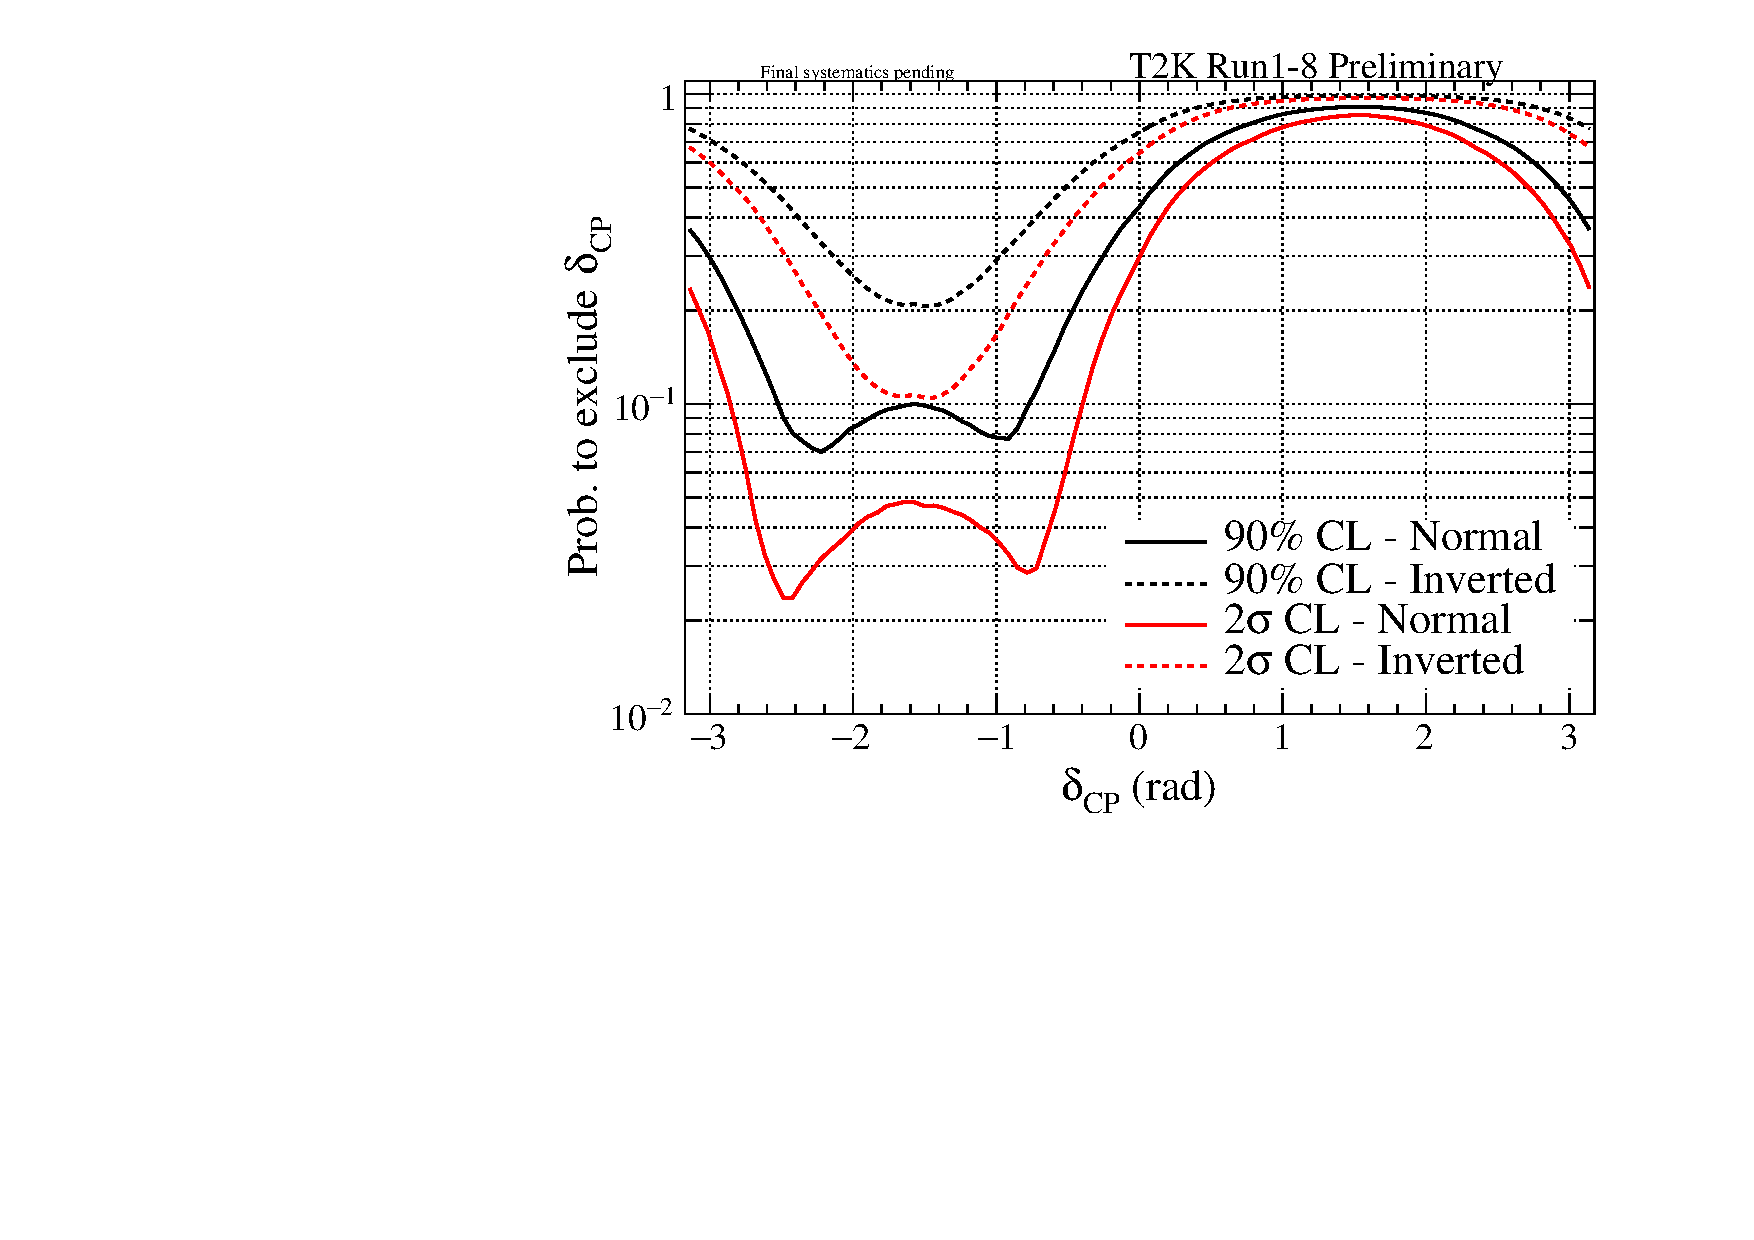
\includegraphics[width=0.9\textwidth]{comparison/dcp_run18_react_Data_prob_chisq}
		\caption{Data \(\Delta \chi^2\) probablility }
	\end{subfigure}
	\caption {
		The distribution of $\Delta\chi^2$ vs \deltacp obtained with \num{1e4} toy experiments generated with $\delta_{CP} = -\pi/2$ and normal hierarchy is shown. The $\Delta\chi^2$ distributions obtained by fixing the mass hierarchy to normal (left) and inverted (right) are shown, along with the $\Delta\chi^2$ values corresponding to 68.27\% and 95.45\% of the toy experiments and the average $\Delta\chi^2$ values from all experiments. Also shown are the fractions of toys which exclude each value of \deltacp to 90\% and $2\sigma$ using the Feldman-Cousins corrected critical values (bottom).
	}
	\label{fig:brazilian_dcp_mpi2}
\end{figure*}

\begin{table}[htb]
	\centering
	\begin{tabular}{| c | c | c | c |}
\hline
\deltacp & Hierarchy & 90\% & $2\sigma$ \\
\hline
0		& NH & 0.430 & 0.300 \\
$\pi$	& NH & 0.383 & 0.250 \\
0		& IH & 0.760 & 0.656 \\
$\pi$	& IH & 0.769 & 0.667 \\
\hline
\end{tabular}

	\caption{
		The fraction of toy experiments for which $\delta_{CP} = 0, \pi$ and normal and inverted hierarchy are excluded at 90\% and $2\sigma$ CL is shown. 10k toy experiments are used.
	}
	\label{tab:exclusion_prob}
\end{table}

\subsubsection{$\delta_{CP} = -1.833$ - normal hierarchy}

In \cref{fig:brazilian_dcp_bestfit} the \RunPeriod data result for \deltacp versus mass hierarchy is compared to the $1\sigma$ and $2\sigma$ uncertainties on the $\Delta\chi^2$ distributions corresponding to $\delta_{CP} = -1.833$ and (a) normal hierarchy and (b) inverted hierarchy. We see that the data contour is consistent with the PMNS matrix at around the $2\sigma$ level.

\begin{figure*}[htb]
	\center
	\begin{subfigure}[b]{0.49\textwidth}
		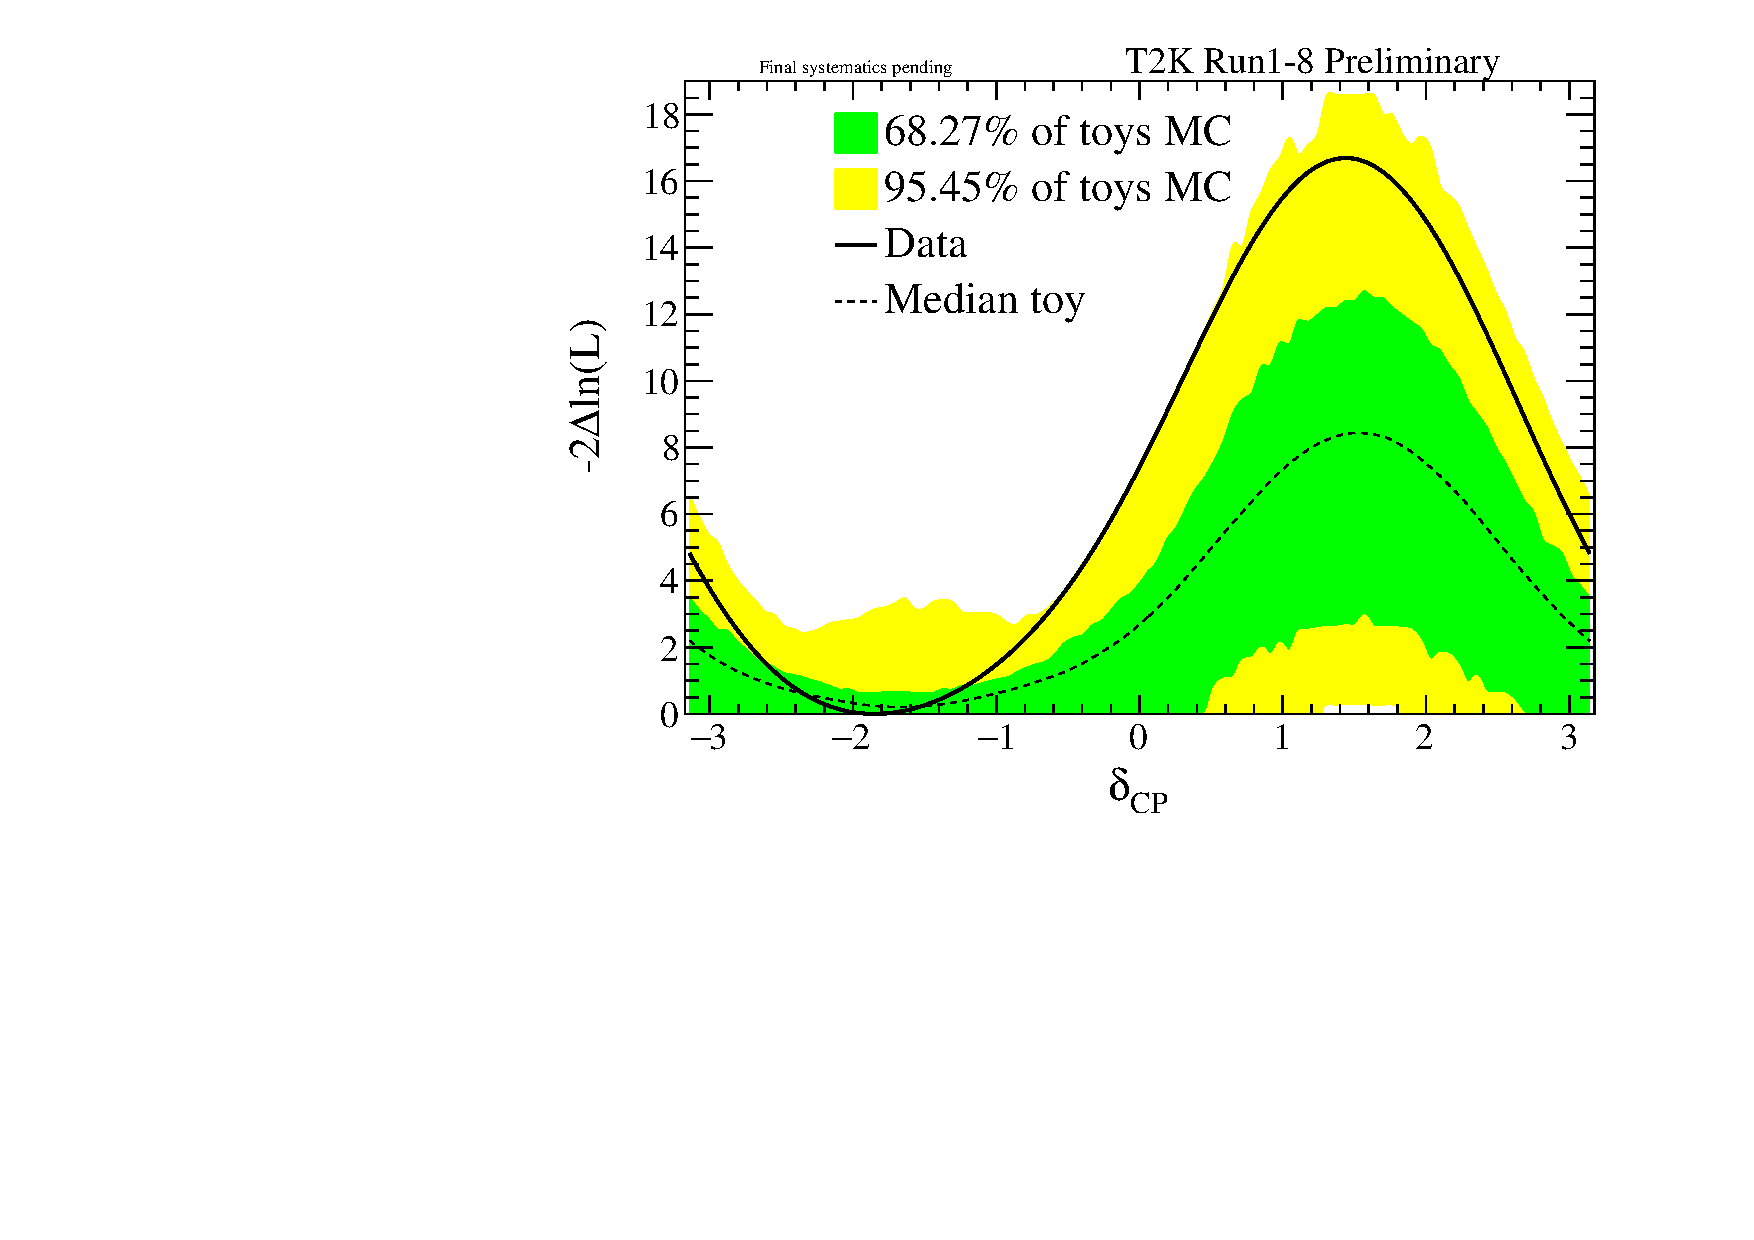
\includegraphics[width=0.9\textwidth]{comparison/deltacp/deltacp_run18_all_twosided_braz_nh}
		\caption{Normal hierarchy}
	\end{subfigure}
	\begin{subfigure}[b]{0.49\textwidth}
		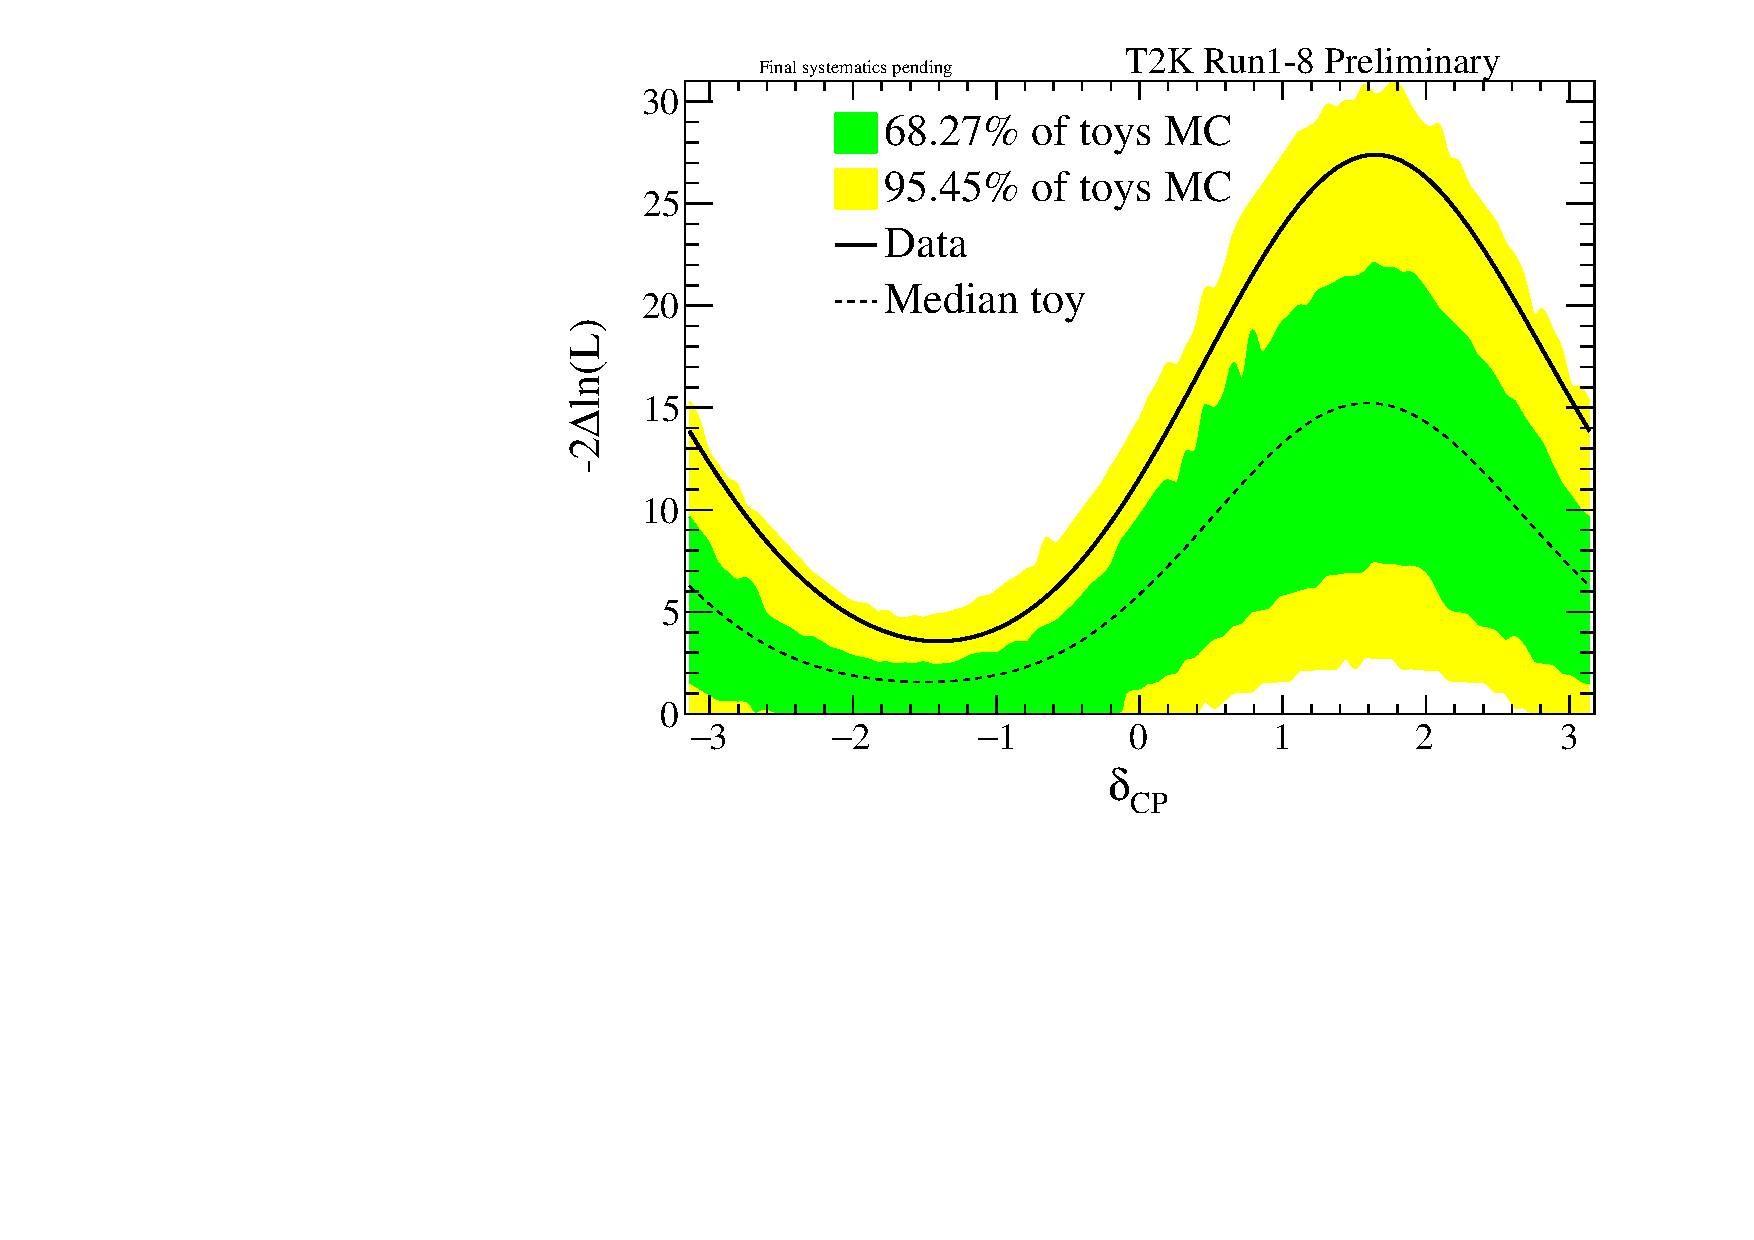
\includegraphics[width=0.9\textwidth]{comparison/deltacp/deltacp_run18_all_twosided_braz_ih}
		\caption{Inverted hierarchy}
	\end{subfigure}
	\caption {
		The distribution of $\Delta\chi^2$ vs \deltacp obtained with \num{1e4} toy experiments generated with $\delta_{CP} = -1,833$ and normal hierarchy is shown. The $\Delta\chi^2$ distributions obtained by fixing the mass hierarchy to normal (left) and inverted (right) are shown, along with the $\Delta\chi^2$ values corresponding to 68.27\% and 95.45\% of the toy experiments, the median toy and the data contour.
	}
	\label{fig:brazilian_dcp_bestfit}
\end{figure*}

\subsubsection{Sample-by-sample expected sensitivity}

An extension to the two-sided method described above was applied in order to assess the effect of each sample on the \deltacp contour obtained. There key difference to the two-sided method described in \cref{sec:results:brazilian:method} is that the generation of the \num{1e4} fake data sets is undertaken for a single sample of interest, with the remaining 4 samples being fixed at the observed spectra.

\Crefrange{fig:brazilian_dcp_nh_samples}{fig:brazilian_dcp_ih_samples}

\begin{figure*}[htb]
	\center
	\begin{subfigure}[b]{0.49\textwidth}
		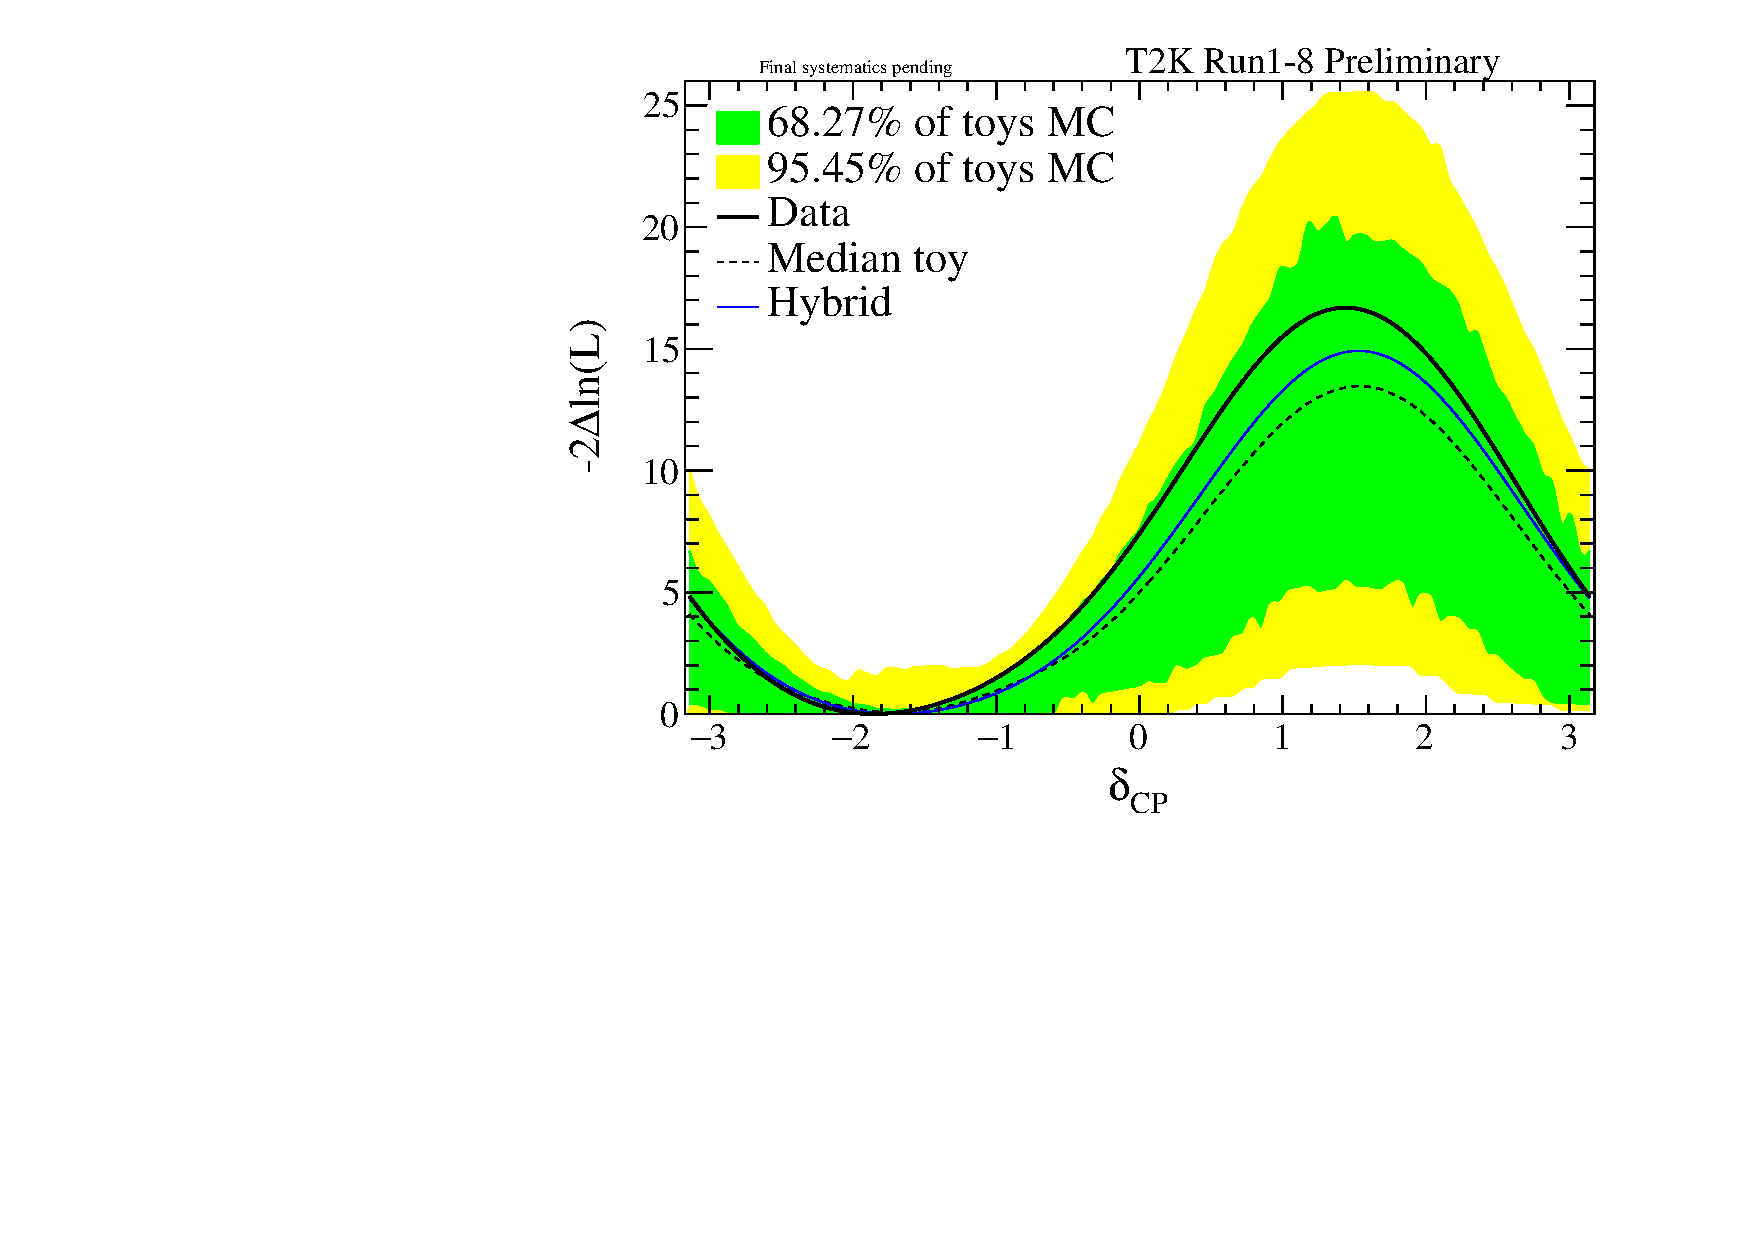
\includegraphics[width=0.9\textwidth]{comparison/deltacp_run18_fhc1re_braz_nh}
		\caption{Electron-like, neutrino mode}
	\end{subfigure}
	\begin{subfigure}[b]{0.49\textwidth}
		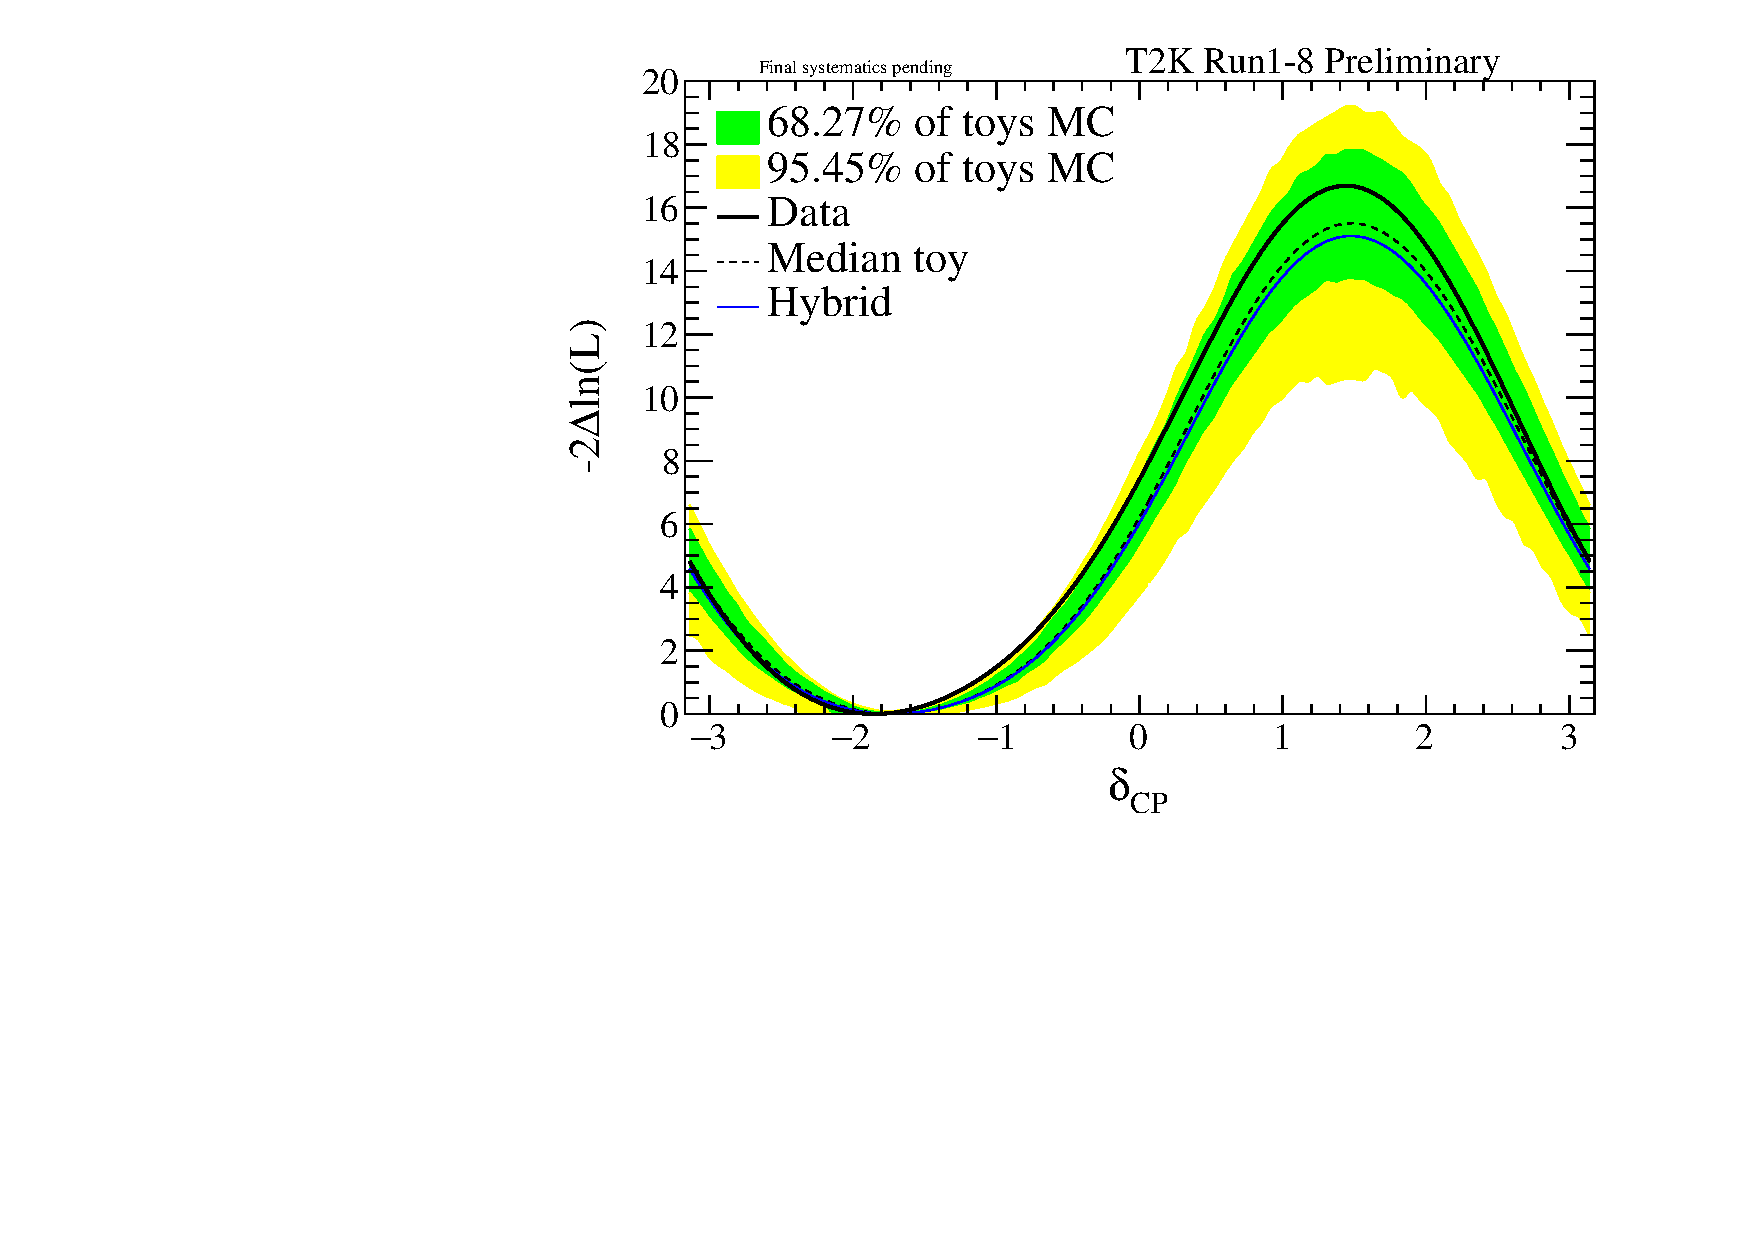
\includegraphics[width=0.9\textwidth]{comparison/deltacp_run18_rhc1re_braz_nh}
		\caption{Electron-like, antineutrino mode}
	\end{subfigure}
	\begin{subfigure}[b]{0.49\textwidth}
		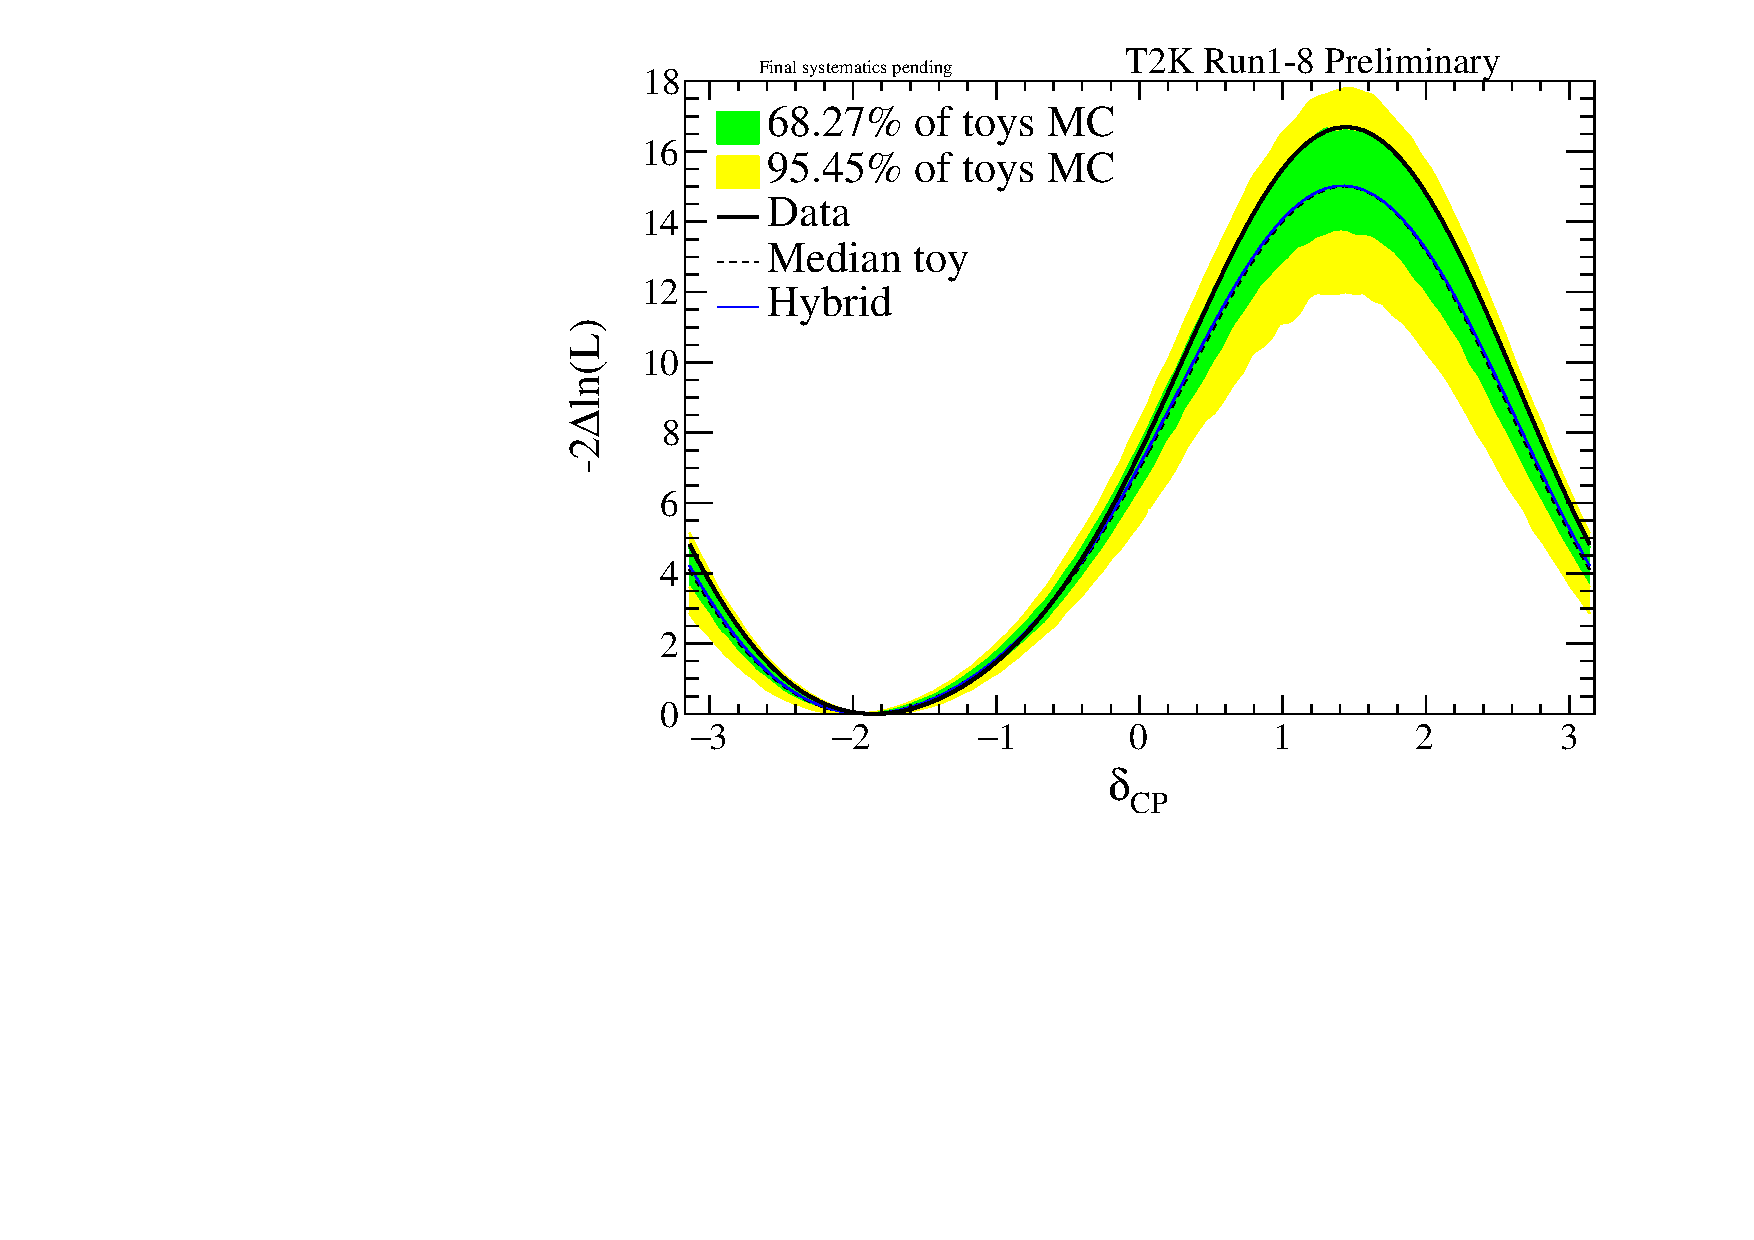
\includegraphics[width=0.9\textwidth]{comparison/deltacp_run18_fhc1rmu_braz_nh}
		\caption{Muon-like, neutrino mode}
	\end{subfigure}
	\begin{subfigure}[b]{0.49\textwidth}
		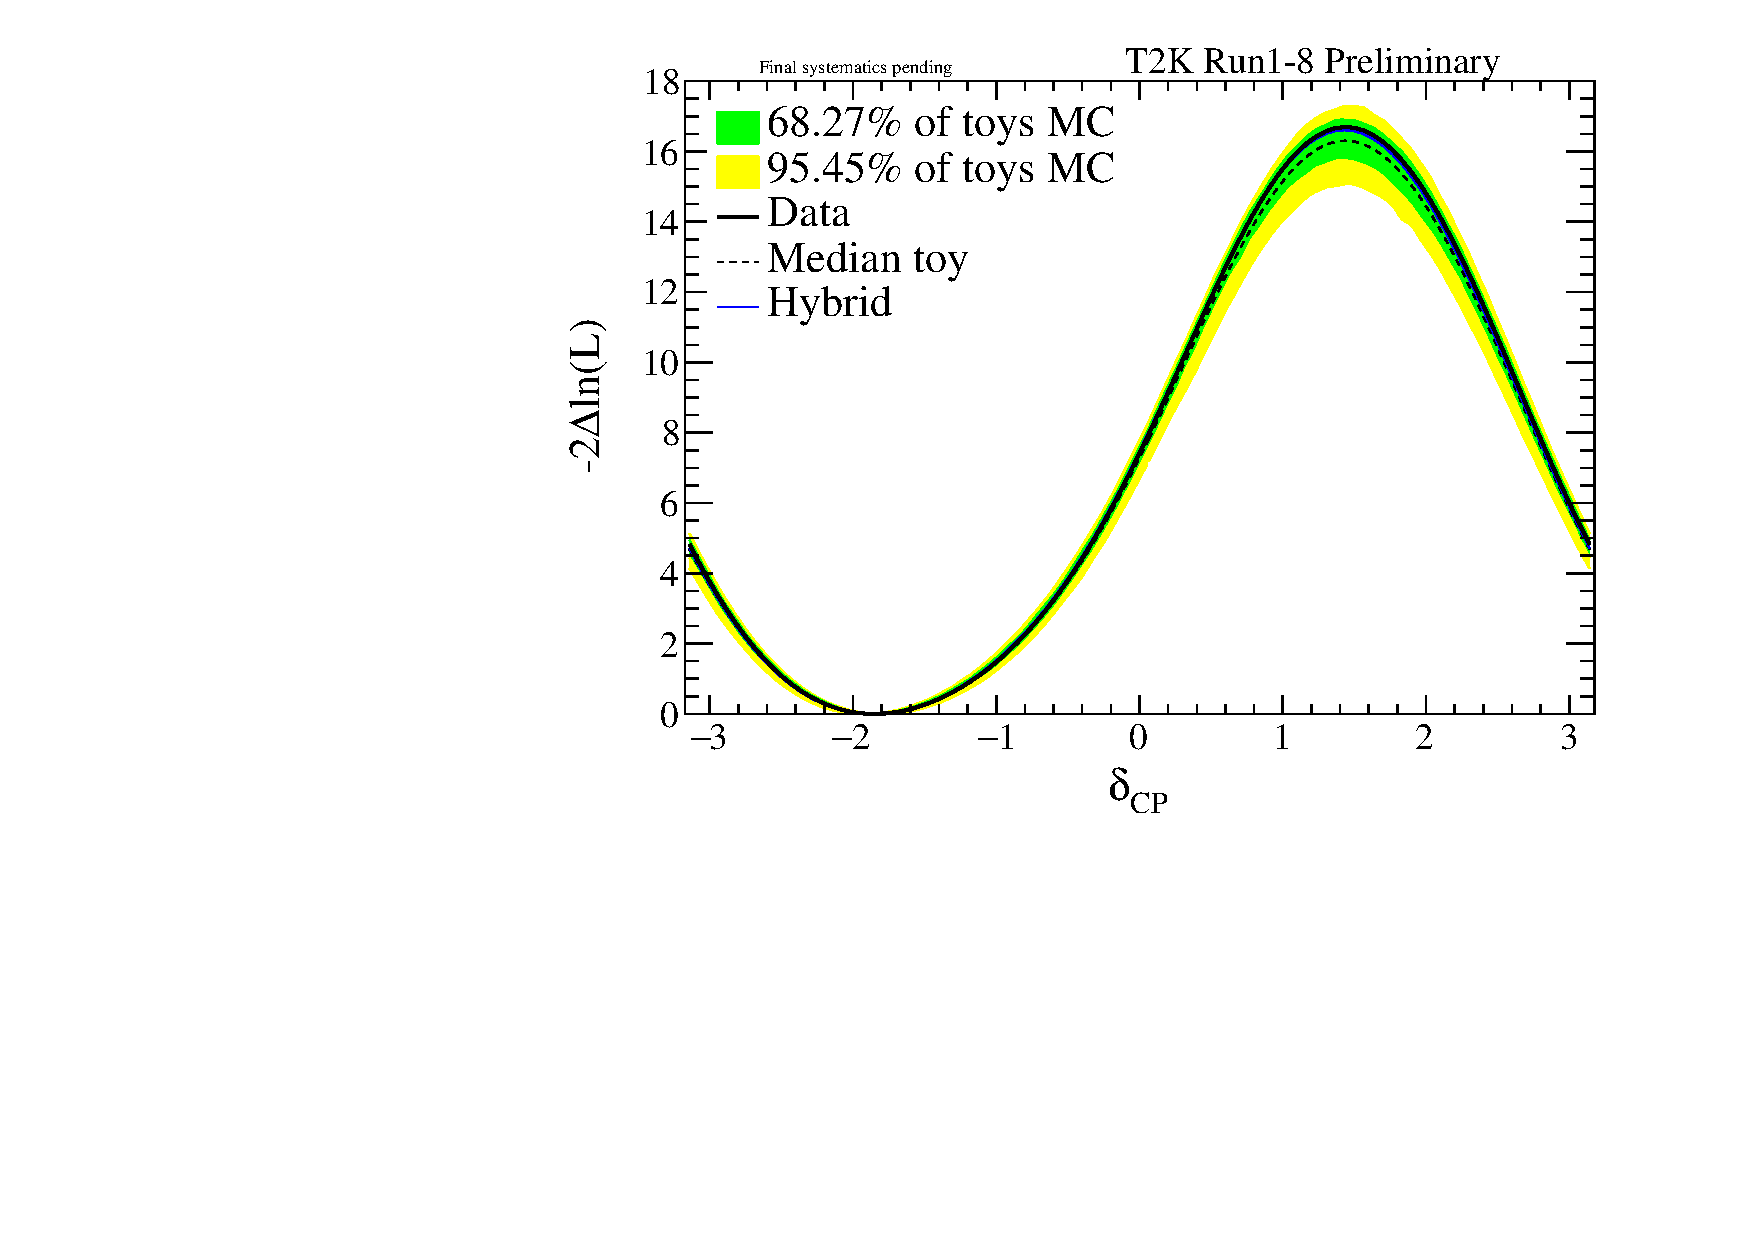
\includegraphics[width=0.9\textwidth]{comparison/deltacp_run18_rhc1rmu_braz_nh}
		\caption{Muon-like, antineutrino mode}
	\end{subfigure}
	\begin{subfigure}[b]{0.49\textwidth}
		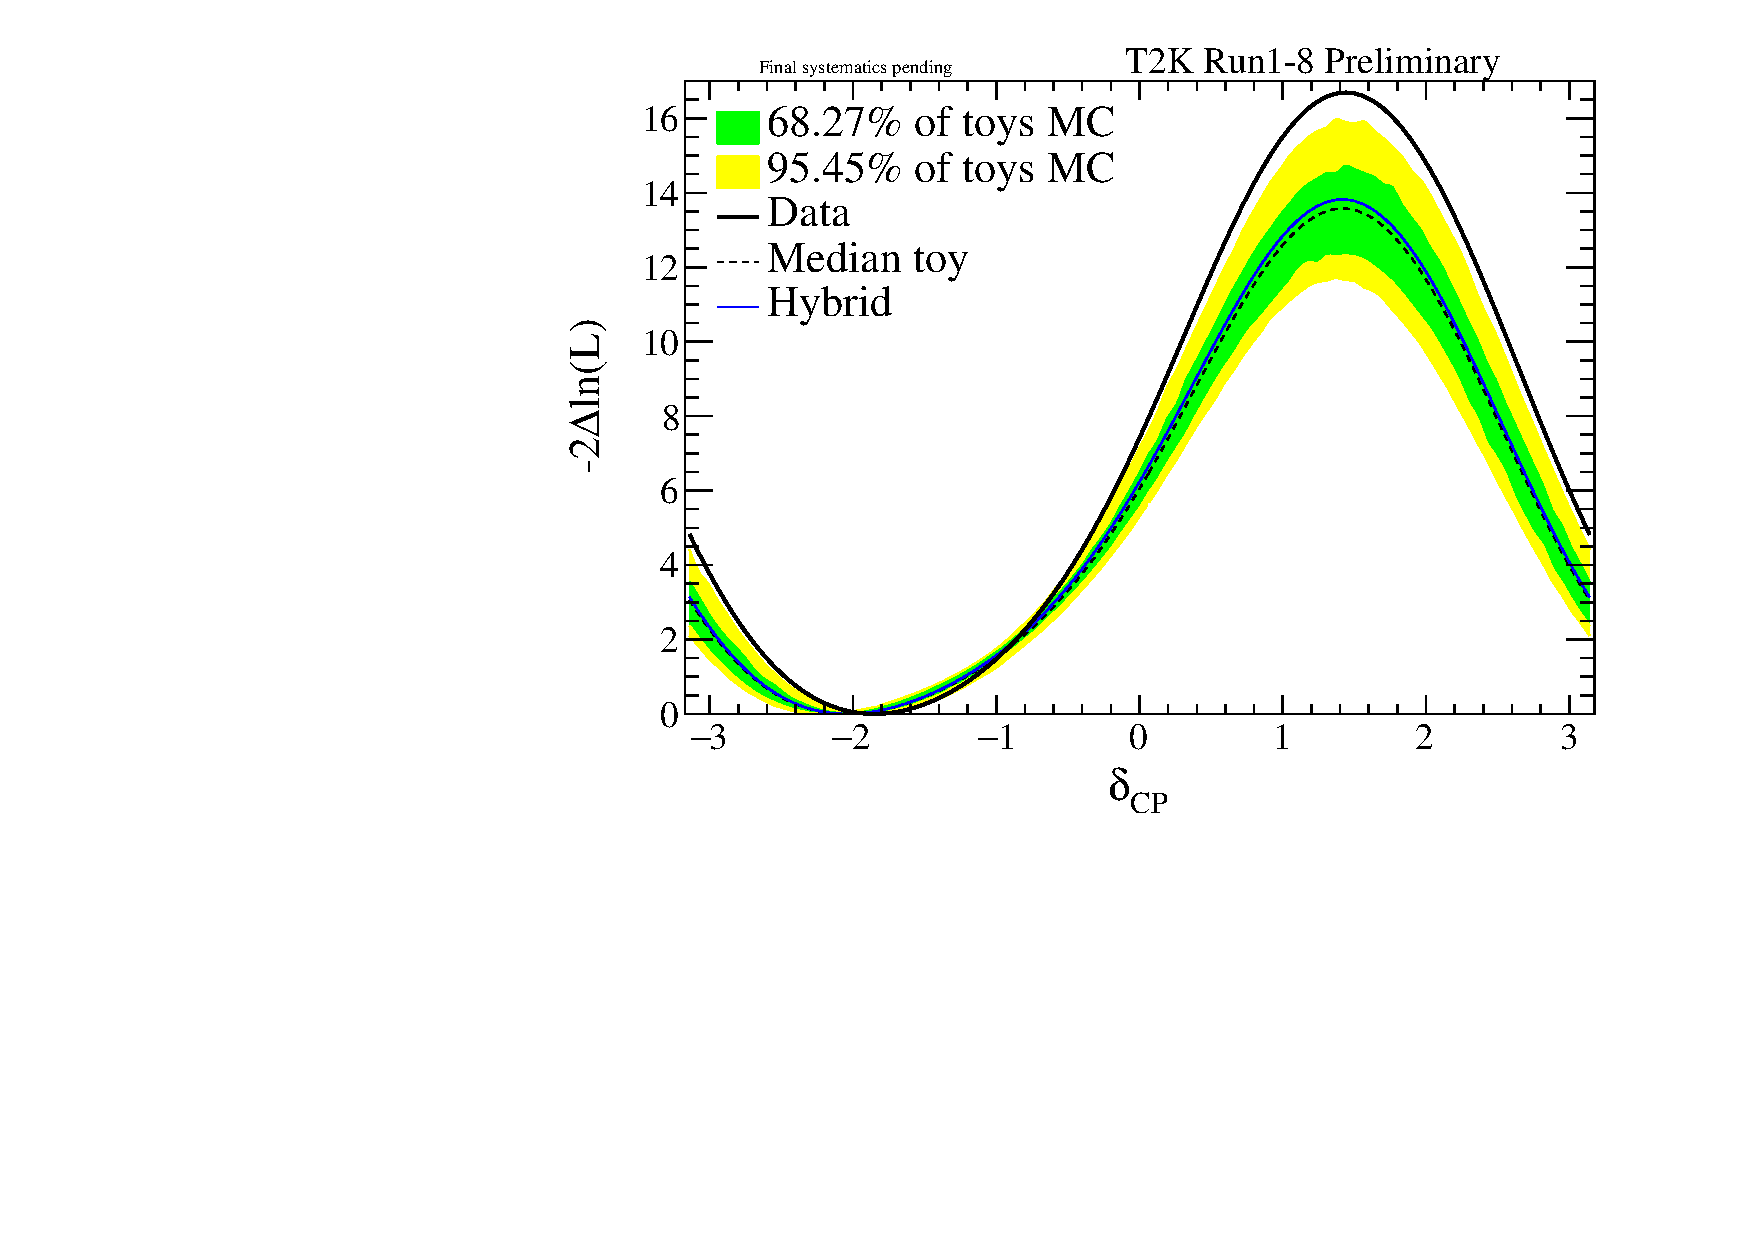
\includegraphics[width=0.9\textwidth]{comparison/deltacp_run18_cc1pi_braz_nh}
		\caption{\nueCConepi-like, neutrino mode}
	\end{subfigure}
	\caption {
		The distribution of $\Delta\chi^2$ vs \deltacp obtained with \num{1e4} toy experiments generated with $\delta_{CP} = -1.833$ and normal hierarchy is shown. The $\Delta\chi^2$ distribution obtained from the full 5-sample fit, obtained by fixing the mass hierarchy to normal, is shown, along with the $\Delta\chi^2$ values corresponding to 68.27\% and 95.45\% of the toy experiments for the indicated sample, with all other samples fixed at their observed spectra.
	}
	\label{fig:brazilian_dcp_nh_samples}
\end{figure*}

\begin{figure*}[htb]
	\center
	\begin{subfigure}[b]{0.49\textwidth}
		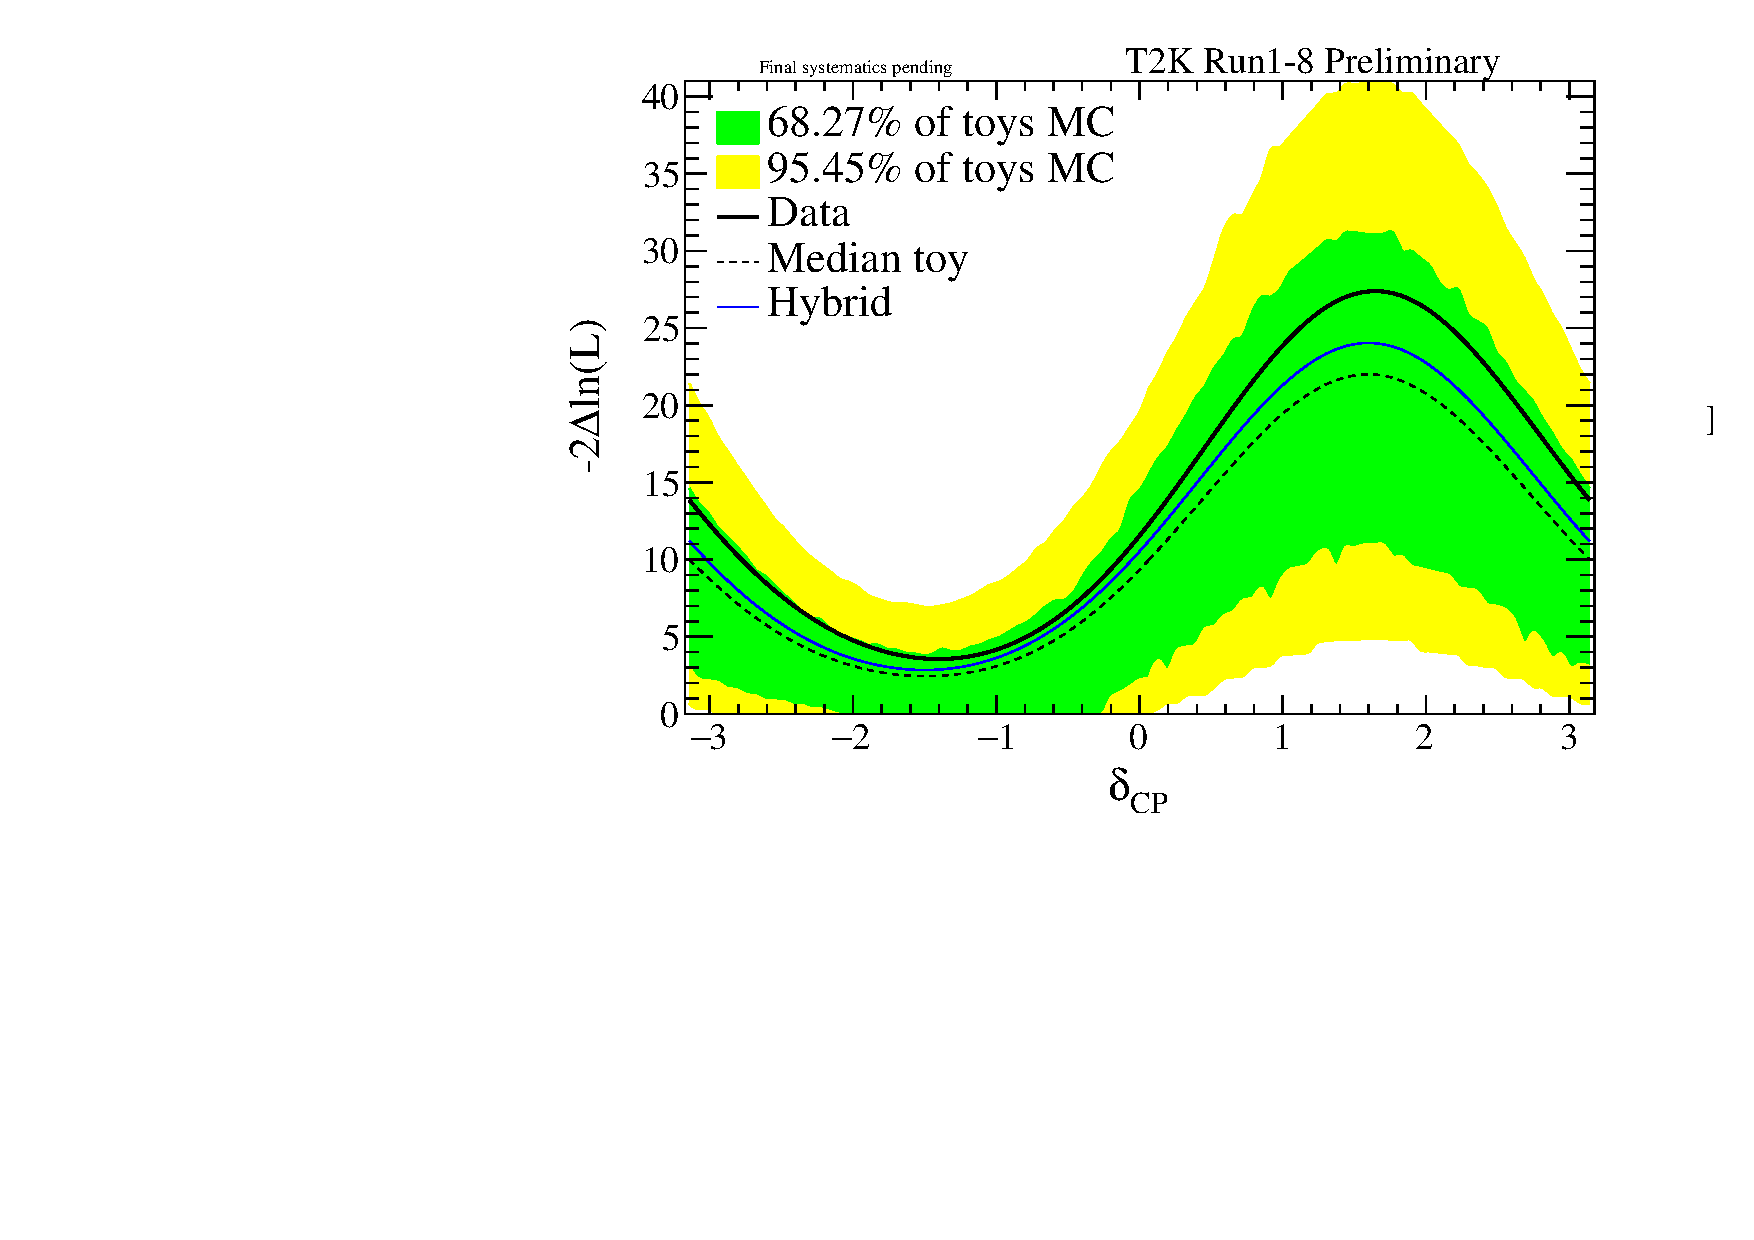
\includegraphics[width=0.9\textwidth]{comparison/deltacp_run18_fhc1re_braz_ih}
		\caption{Electron-like, neutrino mode}
	\end{subfigure}
	\begin{subfigure}[b]{0.49\textwidth}
		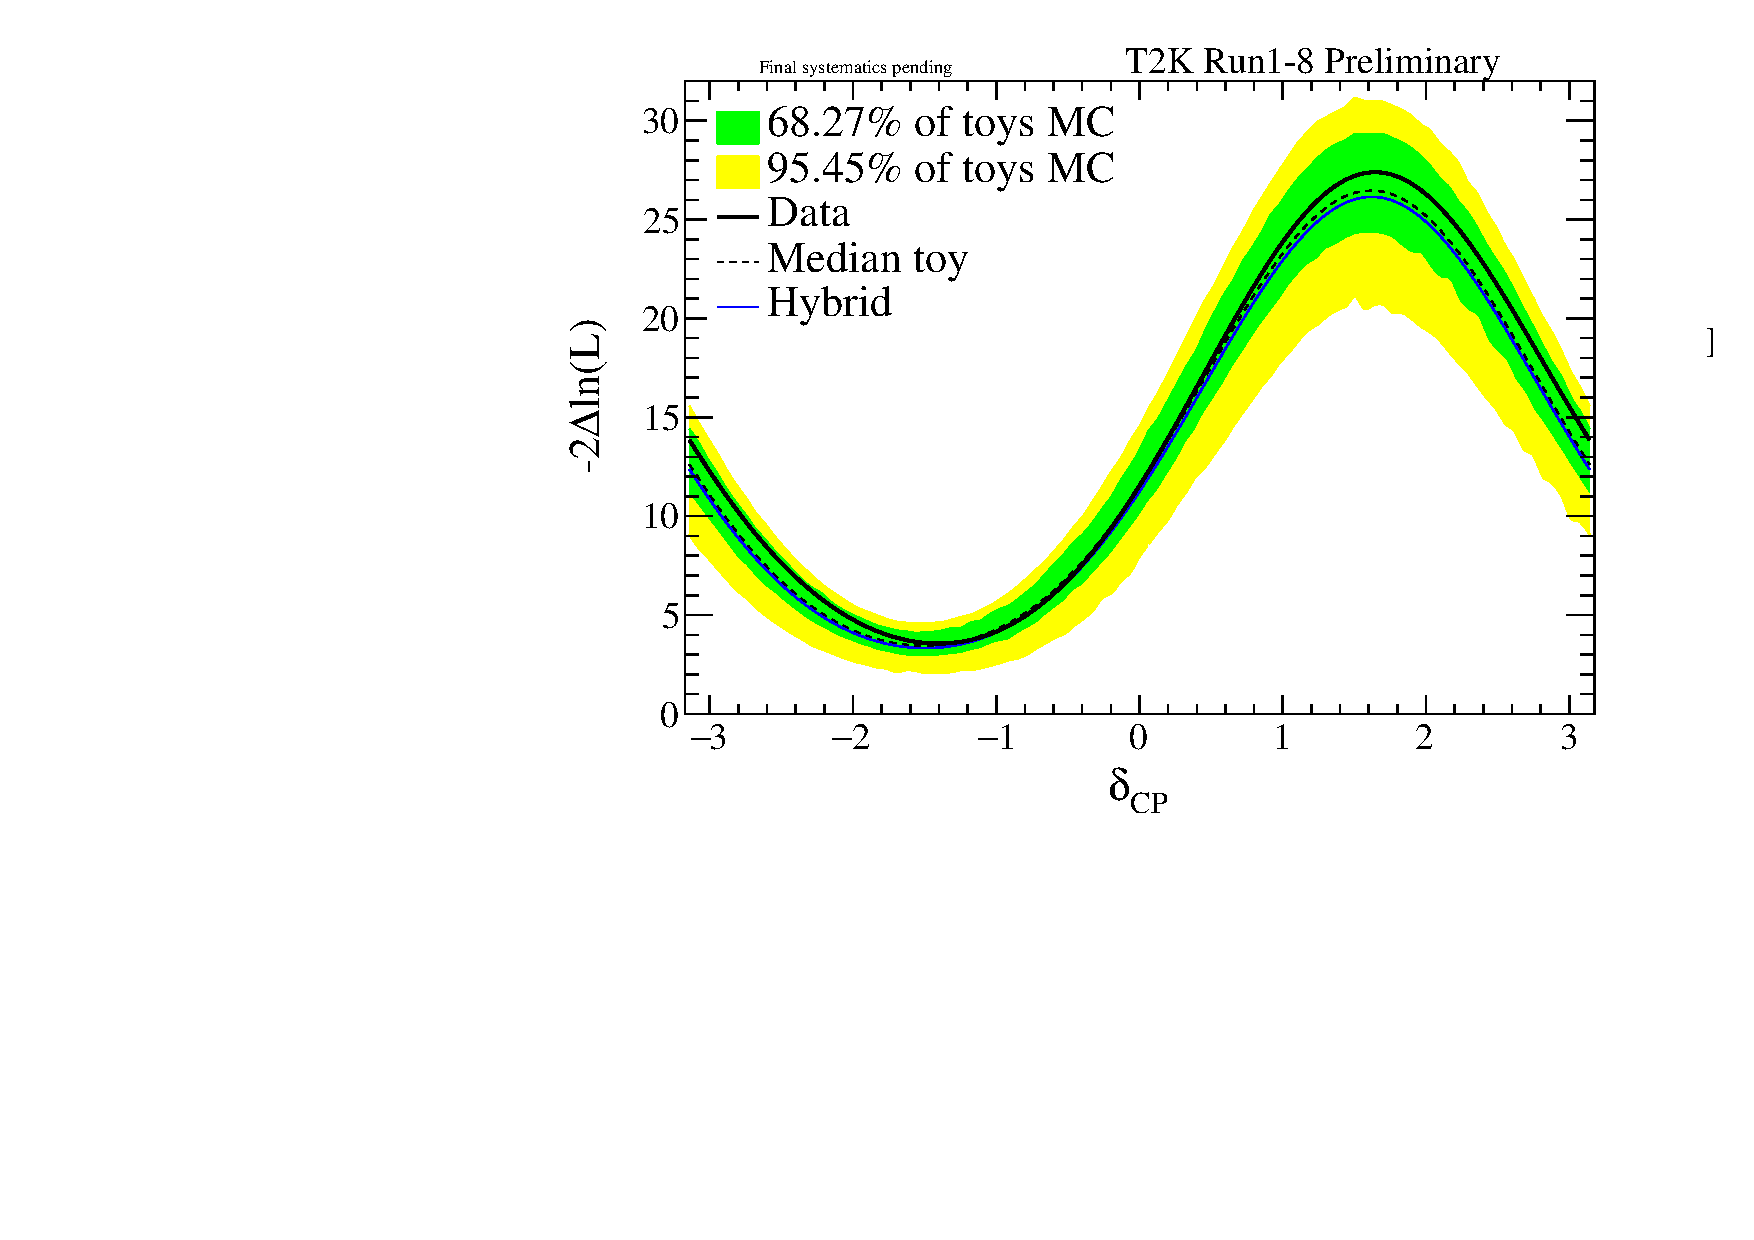
\includegraphics[width=0.9\textwidth]{comparison/deltacp_run18_rhc1re_braz_ih}
		\caption{Electron-like, antineutrino mode}
	\end{subfigure}
	\begin{subfigure}[b]{0.49\textwidth}
		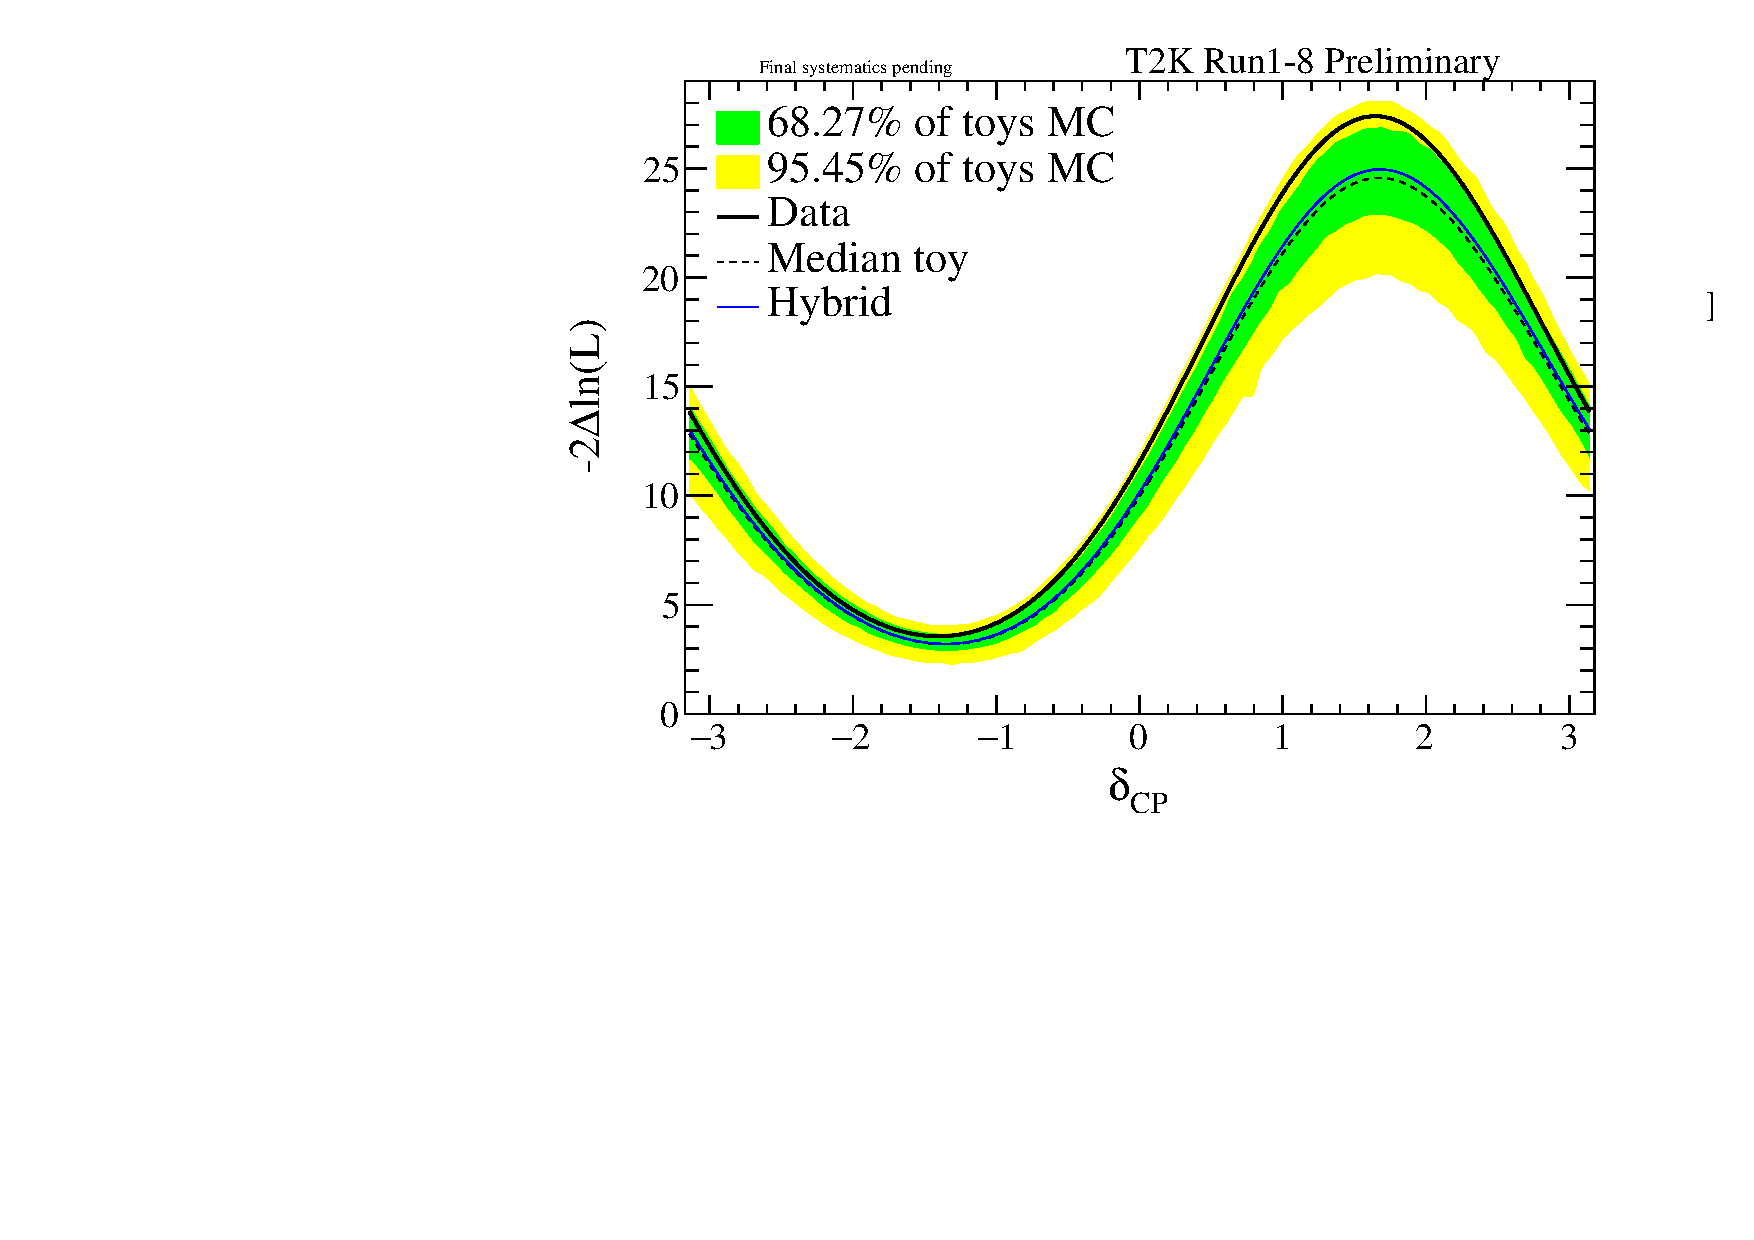
\includegraphics[width=0.9\textwidth]{comparison/deltacp_run18_fhc1rmu_braz_ih}
		\caption{Muon-like, neutrino mode}
	\end{subfigure}
	\begin{subfigure}[b]{0.49\textwidth}
		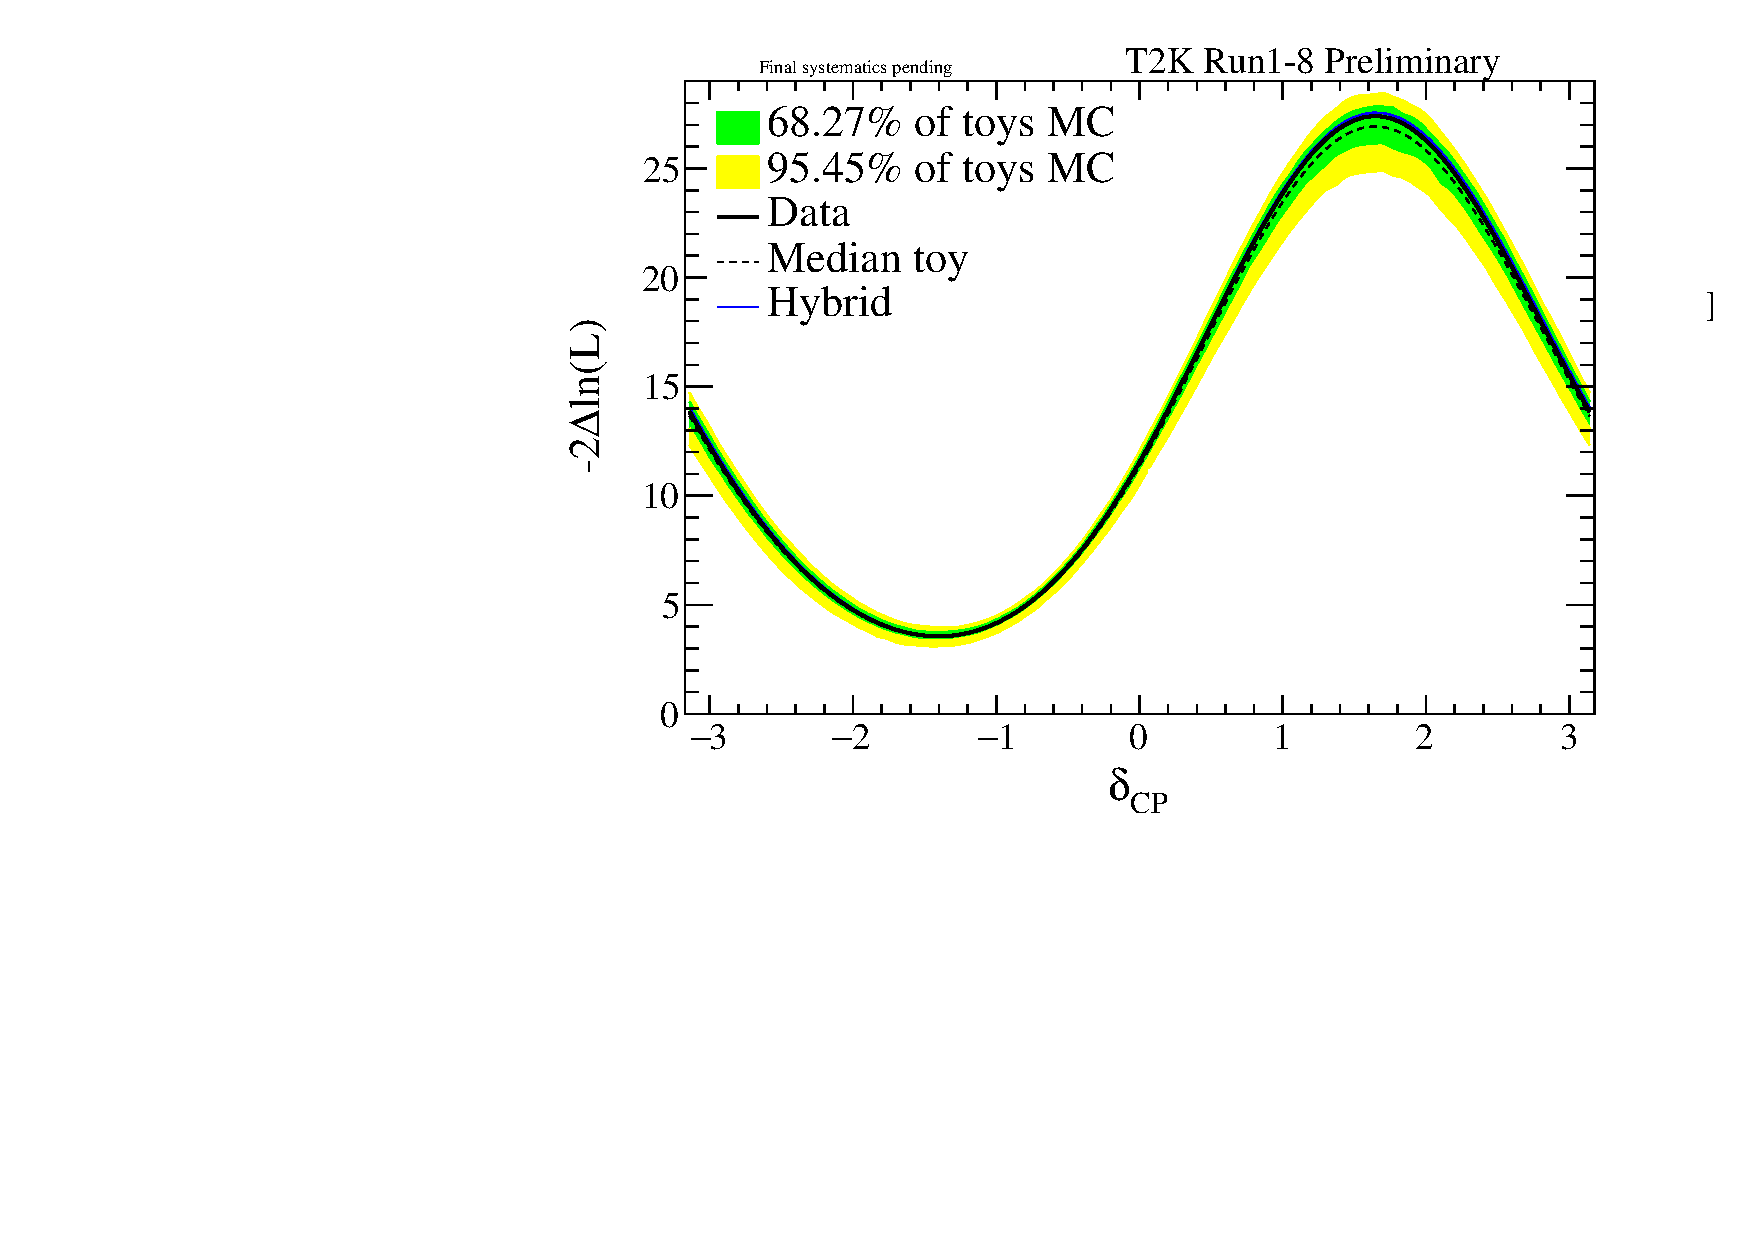
\includegraphics[width=0.9\textwidth]{comparison/deltacp_run18_rhc1rmu_braz_ih}
		\caption{Muon-like, antineutrino mode}
	\end{subfigure}
	\begin{subfigure}[b]{0.49\textwidth}
		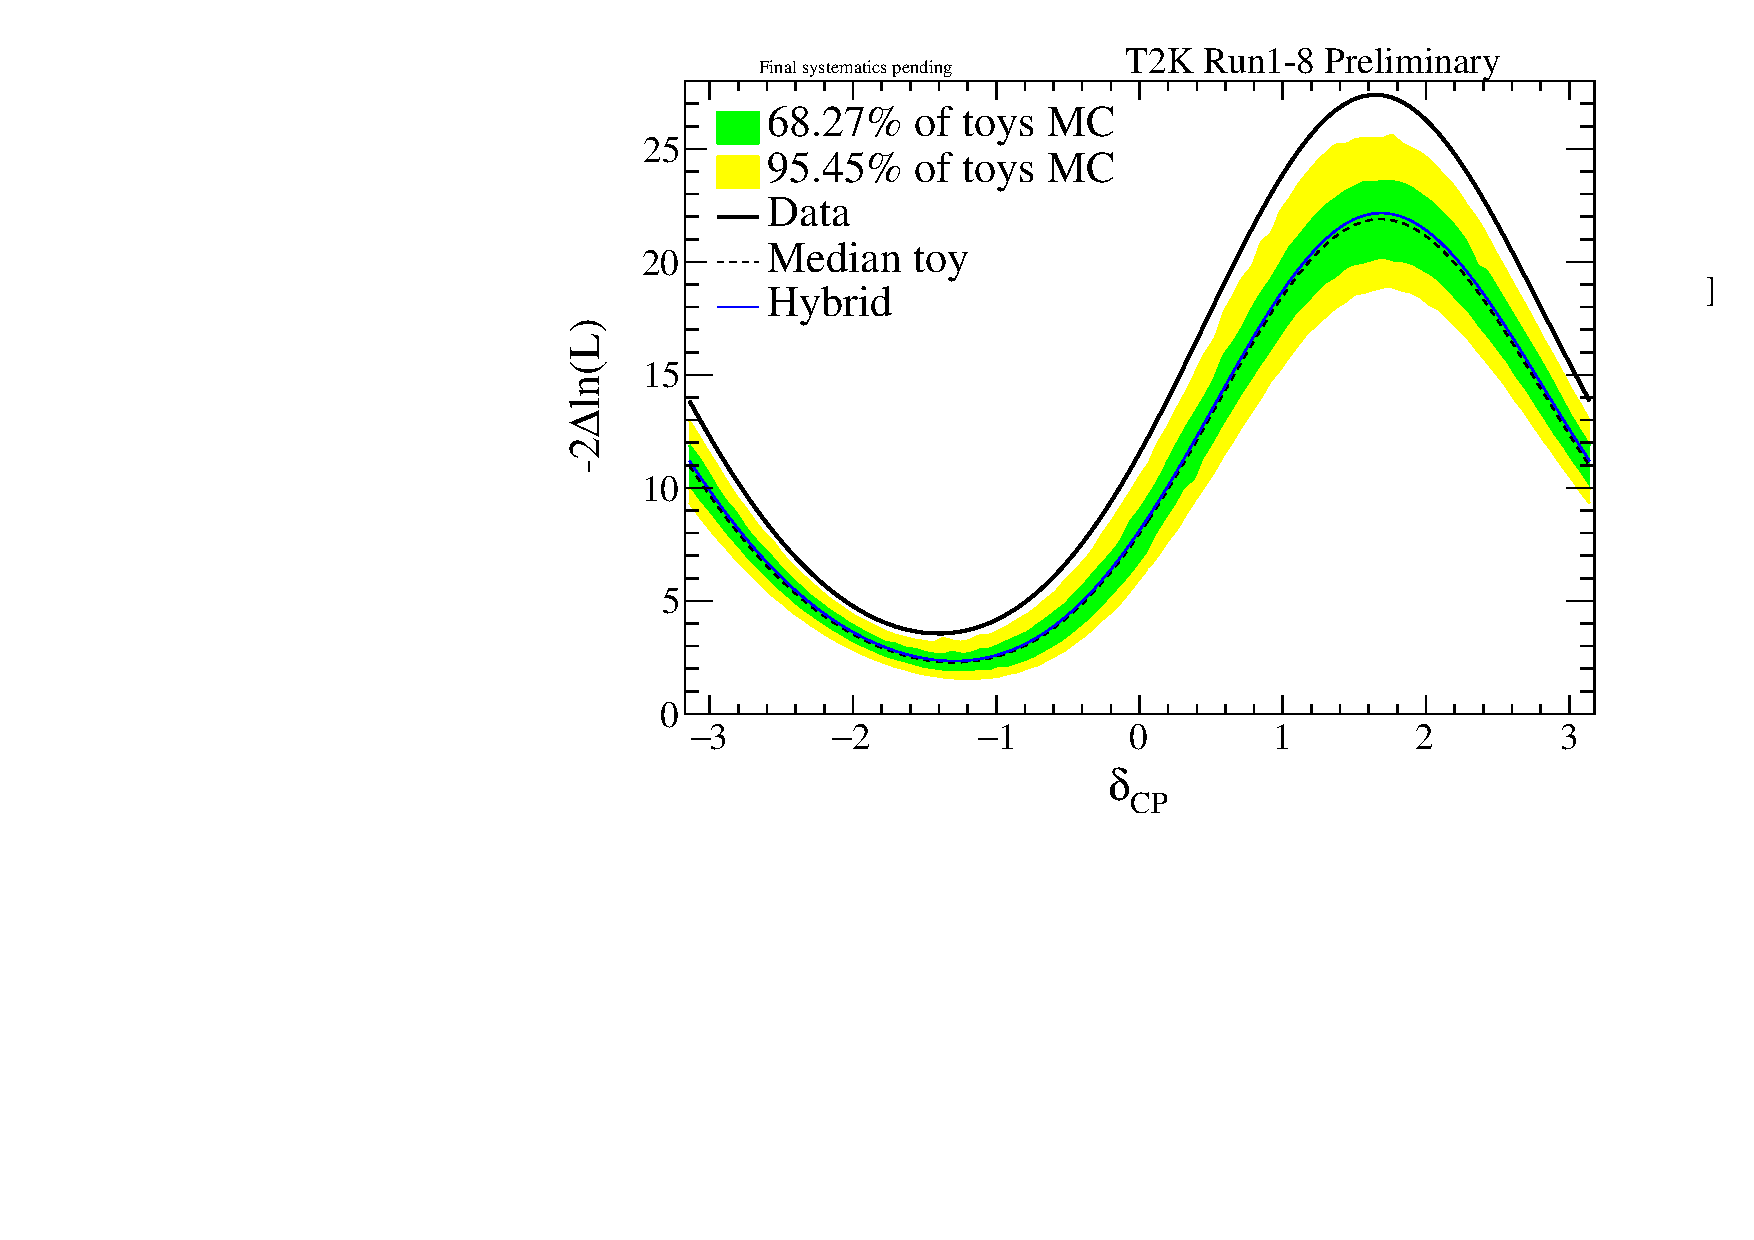
\includegraphics[width=0.9\textwidth]{comparison/deltacp_run18_cc1pi_braz_ih}
		\caption{\nueCConepi-like, neutrino mode}
	\end{subfigure}
	\caption {
		The distribution of $\Delta\chi^2$ vs \deltacp obtained with \num{1e4} toy experiments generated with $\delta_{CP} = -1.833$ and normal hierarchy is shown. The $\Delta\chi^2$ distribution obtained from the full 5-sample fit, obtained by fixing the mass hierarchy to inverted, is shown, along with the $\Delta\chi^2$ values corresponding to 68.27\% and 95.45\% of the toy experiments for the indicated sample, with all other samples fixed at their observed spectra.
	}
	\label{fig:brazilian_dcp_ih_samples}
\end{figure*}

It can be seen from \cref{fig:brazilian_dcp_nh_samples} that for normal hierarchy the observed contour resides within the $1\sigma$ band of expected sensitivities for 4 of the samples and thus while three of these contours are contributing to a stronger constraint than expected, the additional strength of the constraint in these samples is by no means surprising.

The contribution from the \nueCConepi sample is rather extreme, as might be expected given the excess events observed in this sample, with the observed contour falling outside the $2\sigma$ band of expected sensitivities for this sample. Nonetheless, with all 5 samples considered together, as in \cref{fig:brazilian_dcp_mpi2}(a), the observed constraint resides approximately within the $2\sigma$ expected sensitivity.

For the case of inverted hierarchy (\cref{fig:brazilian_dcp_ih_samples}) a similar scenario is observed, the principal difference being that the FHC one-ring $\mu$-like sample has an observed contour contained with the $2\sigma$ band of expected sensitivities, though the full 5 sample contour remains within the $2\sigma$ expected sensitivity (\cref{fig:brazilian_dcp_mpi2}).

\subsection {Comparison of \ssqthtwothree versus mass hierarchy result with sensitivity}
\label{sec:results:brazilian_mixing23}

This section provides a comparison of the \RunPeriod data fit with the expected sensitivity for \ssqthtwothree.

The procedure used is the one outline in \cref{sec:results:brazilian:method} for the two-sided distribution, with the appropriate change in oscillation parameter. Furthermore, whereas the expected sensitivity method for \deltacp throws the atmospheric parameters from a 2D likelihood distribution from on an Asimov fake data set, whose oscillation parameter values are those from the disappearance data fit, in this case the \dmsqtwothree parameter is thrown from the 1D projection of this likelihood distribution.

\subsubsection{$\sin^2\theta_{23} = 0.530$ - normal hierarchy}

In \cref{fig:brazilian_mixing23_bestfit} the \RunPeriod data result for \ssqthtwothree versus mass hierarchy is compared to the $1\sigma$ and $2\sigma$ uncertainties on the $\Delta\chi^2$ distributions corresponding to $\sin^2\theta_{23} = 0.530$ for (a) normal hierarchy and (b) inverted hierarchy.

\begin{figure*}[htb]
	\center
	\begin{subfigure}[b]{0.49\textwidth}
		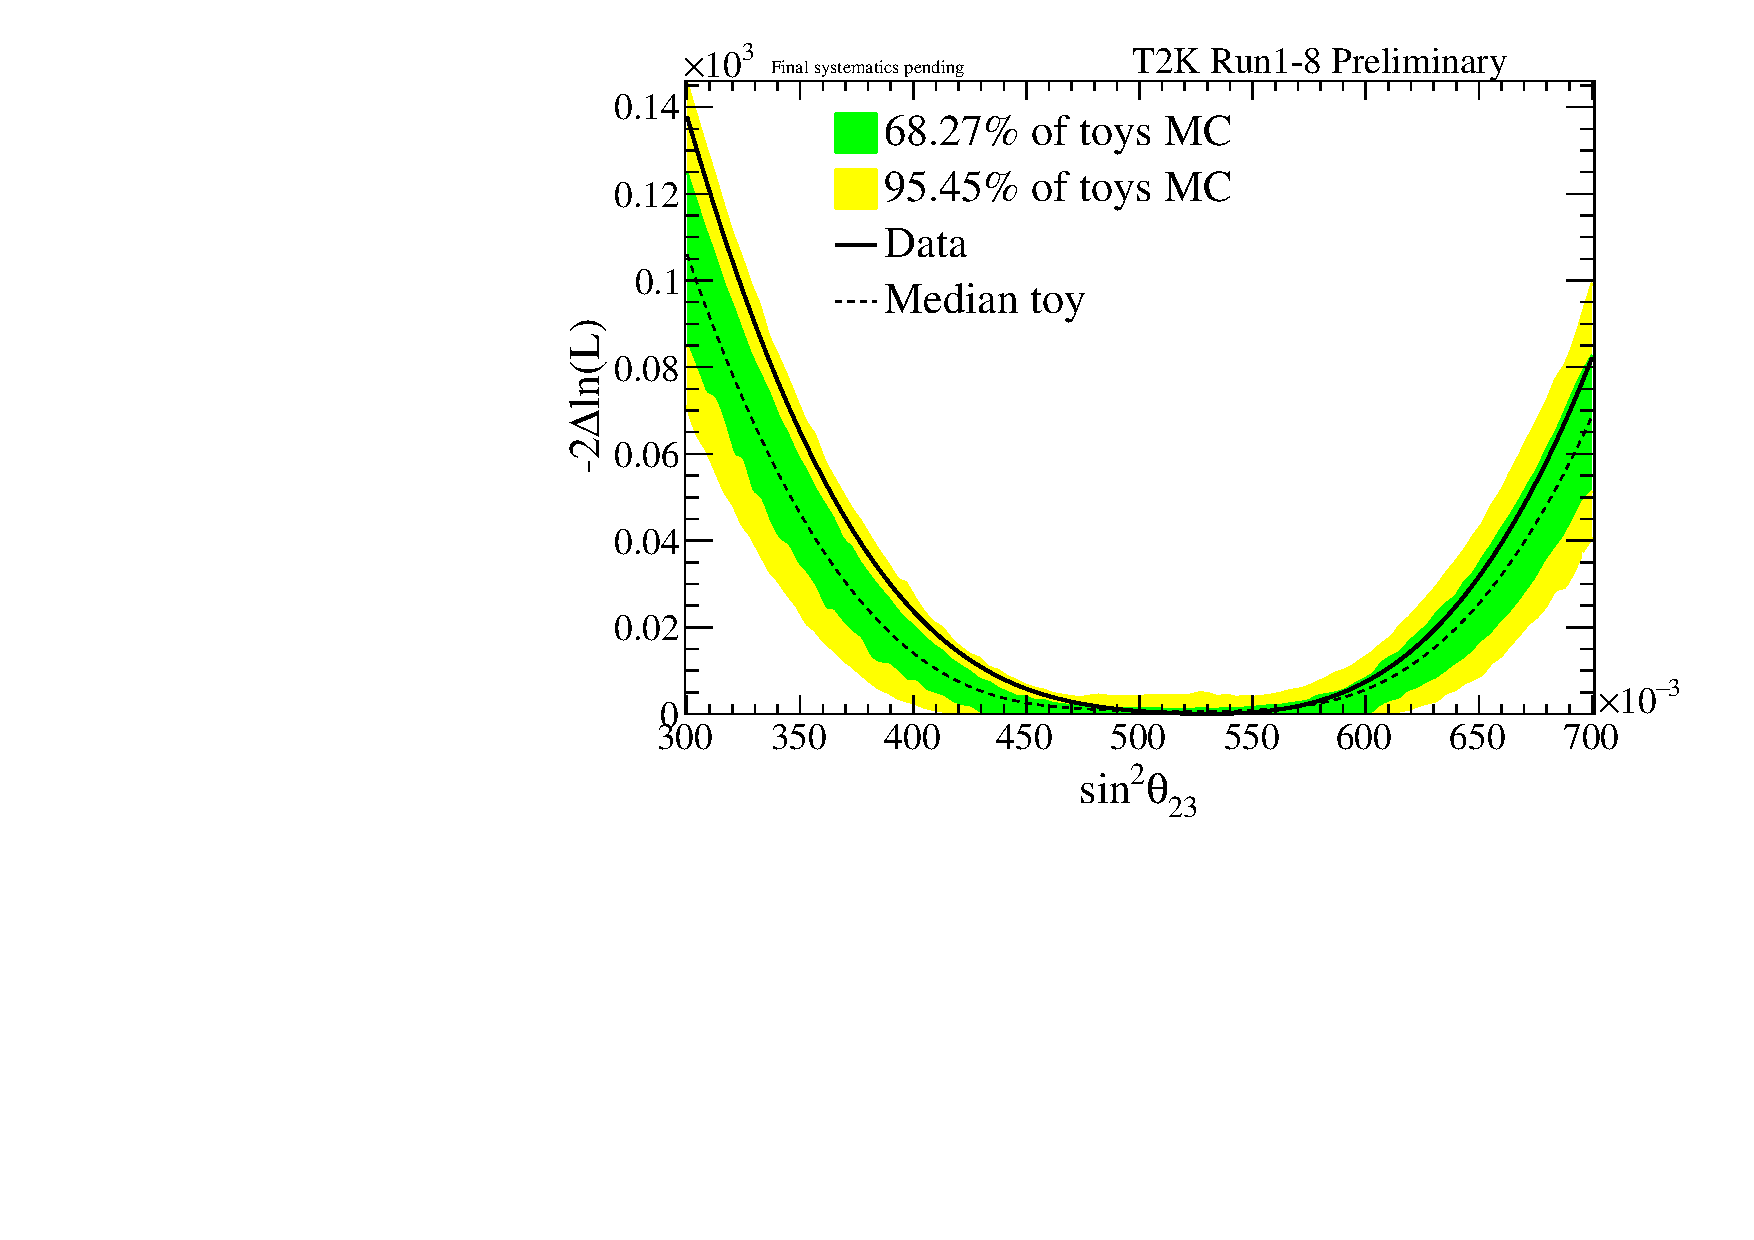
\includegraphics[width=0.9\textwidth]{comparison/mixing23/mixing23_run18_all_twosided_braz_nh}
		\caption{Normal hierarchy}
	\end{subfigure}
	\begin{subfigure}[b]{0.49\textwidth}
		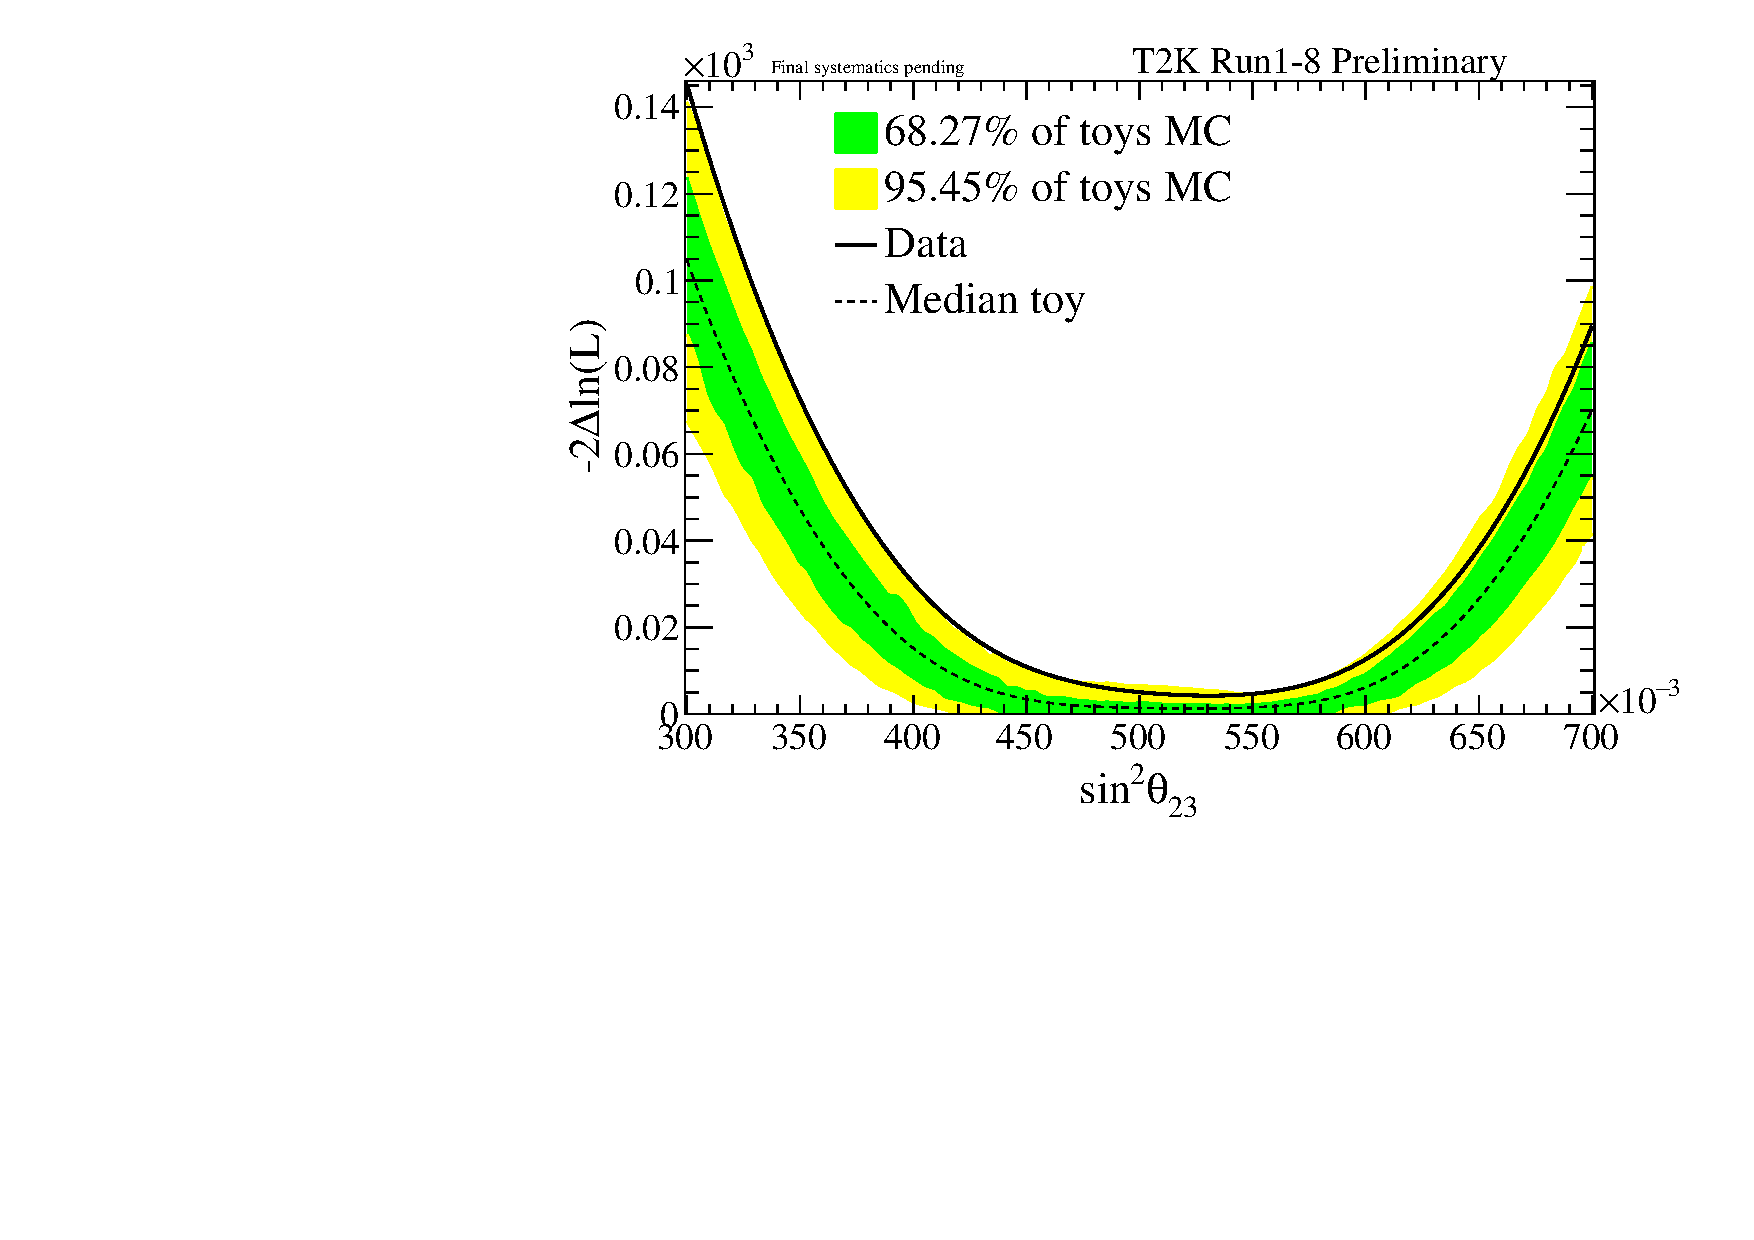
\includegraphics[width=0.9\textwidth]{comparison/mixing23/mixing23_run18_all_twosided_braz_ih}
		\caption{Inverted hierarchy}
	\end{subfigure}
	\caption {
		The distribution of $\Delta\chi^2$ vs \ssqthtwothree obtained with \num{1e4} toy experiments generated with $\sin^2\theta_{23} = 0.530$ and normal hierarchy is shown. The $\Delta\chi^2$ distributions obtained by fixing the mass hierarchy to normal (left) and inverted (right) are shown, along with the $\Delta\chi^2$ values corresponding to 68.27\% and 95.45\% of the toy experiments, the median toy and the data contour.
	}
	\label{fig:brazilian_mixing23_bestfit}
\end{figure*}

\subsection {Comparison of \dmsqtwothree versus mass hierarchy result with sensitivity}
\label{sec:results:brazilian_dmsq}

This section provides a comparison of the \RunPeriod data fit with the expected sensitivity for \dmsqtwothree.

The procedure used is the one outline in \cref{sec:results:brazilian:method} for the two-sided distribution, with the appropriate change in oscillation parameter. Furthermore, whereas the expected sensitivity method for \deltacp throws the atmospheric parameters from a 2D likelihood distribution from on an Asimov fake data set, whose oscillation parameter values are those from the disappearance data fit, in this case the \ssqthtwothree parameter is thrown from the 1D projection of this likelihood distribution.

\subsubsection{$\Delta m^2_{32} = -2.462 \times 10^{-3} \text{eV}^2\text{ c}^{-4}$ - normal hierarchy}

In \cref{fig:brazilian_dmsq23_bestfit} the \RunPeriod data result for \dmsqtwothree versus mass hierarchy is compared to the $1\sigma$ and $2\sigma$ uncertainties on the $\Delta\chi^2$ distributions corresponding to $\Delta m^2_{32} = -2.462 \times 10^{-3} \text{eV}^2\text{ c}^{-4}$ for (a) normal hierarchy and (b) inverted hierarchy.

\begin{figure*}[htb]
	\center
	\begin{subfigure}[b]{0.49\textwidth}
		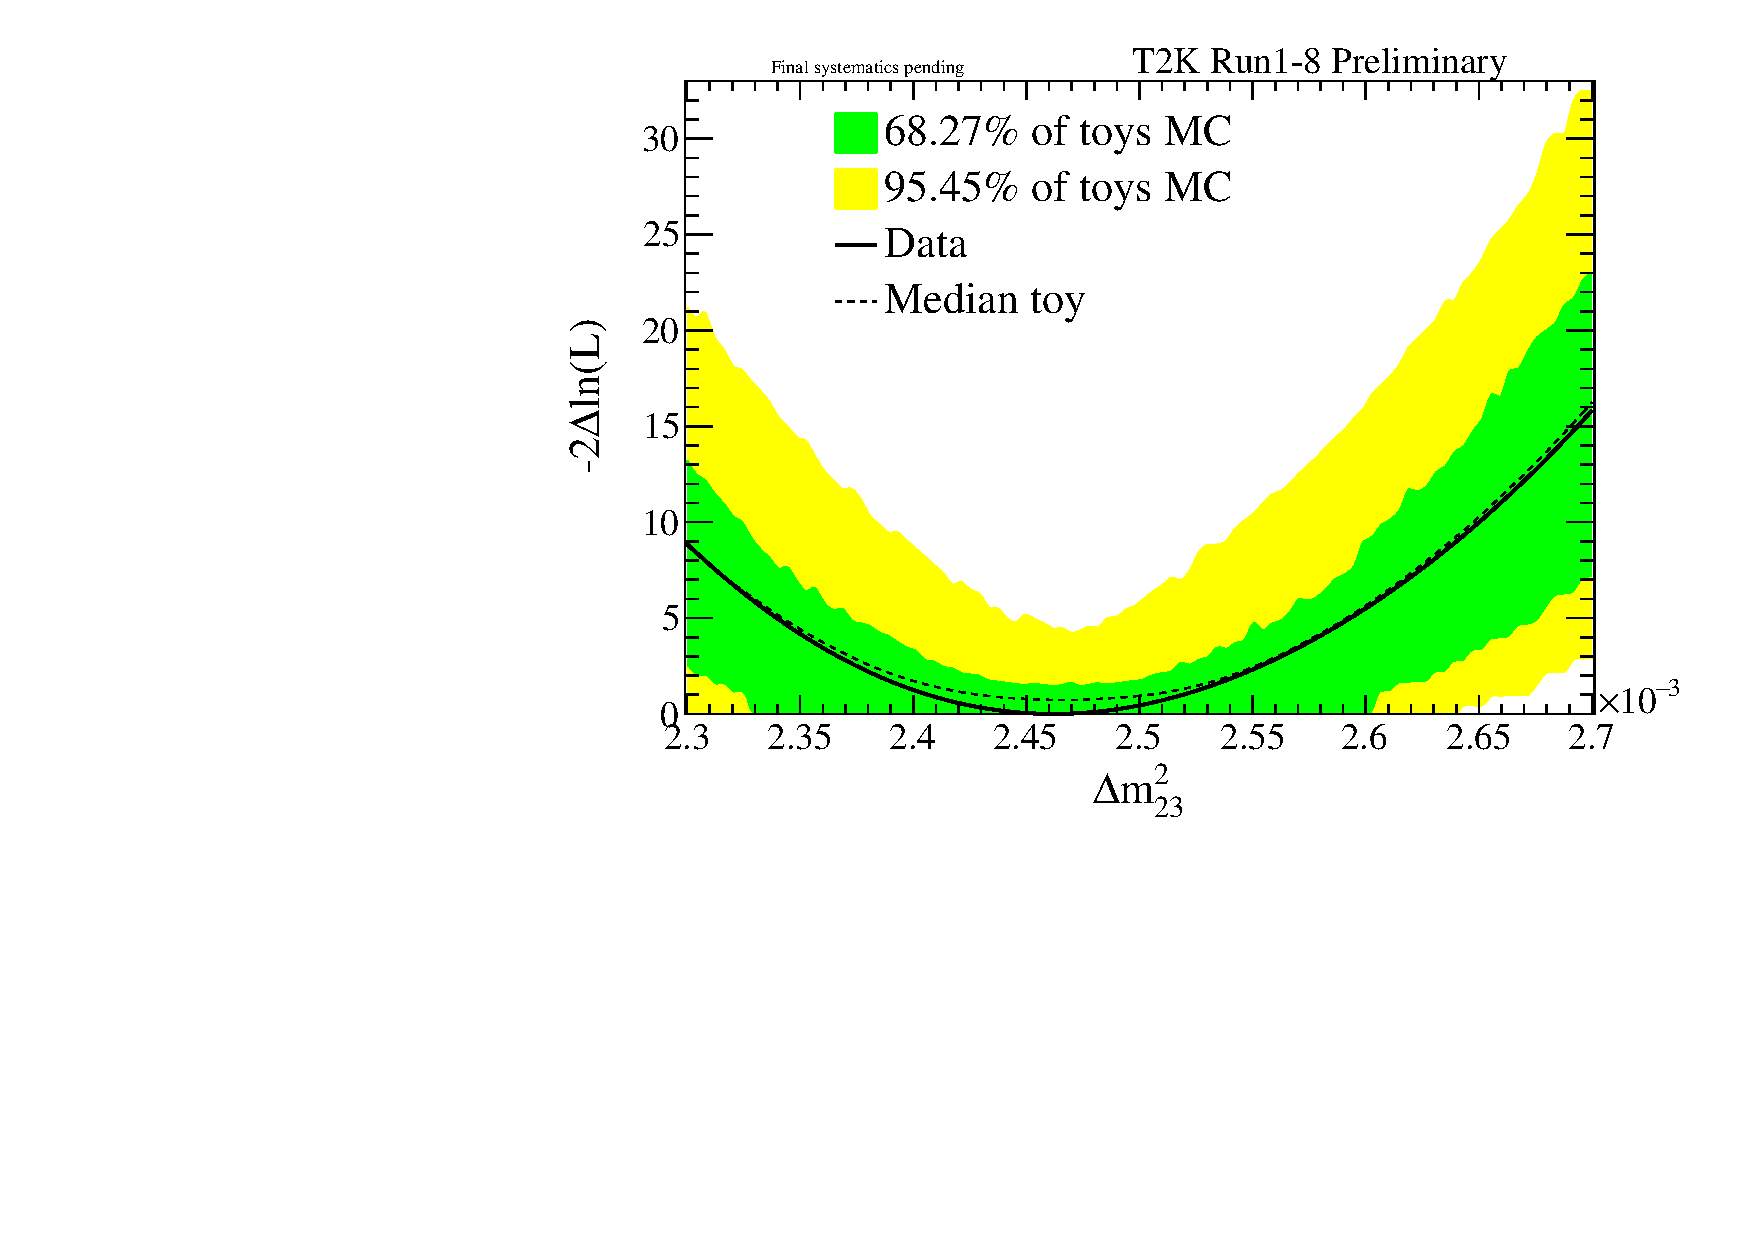
\includegraphics[width=0.9\textwidth]{comparison/dmsq23/dmsq23_run18_all_twosided_braz_nh}
		\caption{Normal hierarchy}
	\end{subfigure}
	\begin{subfigure}[b]{0.49\textwidth}
		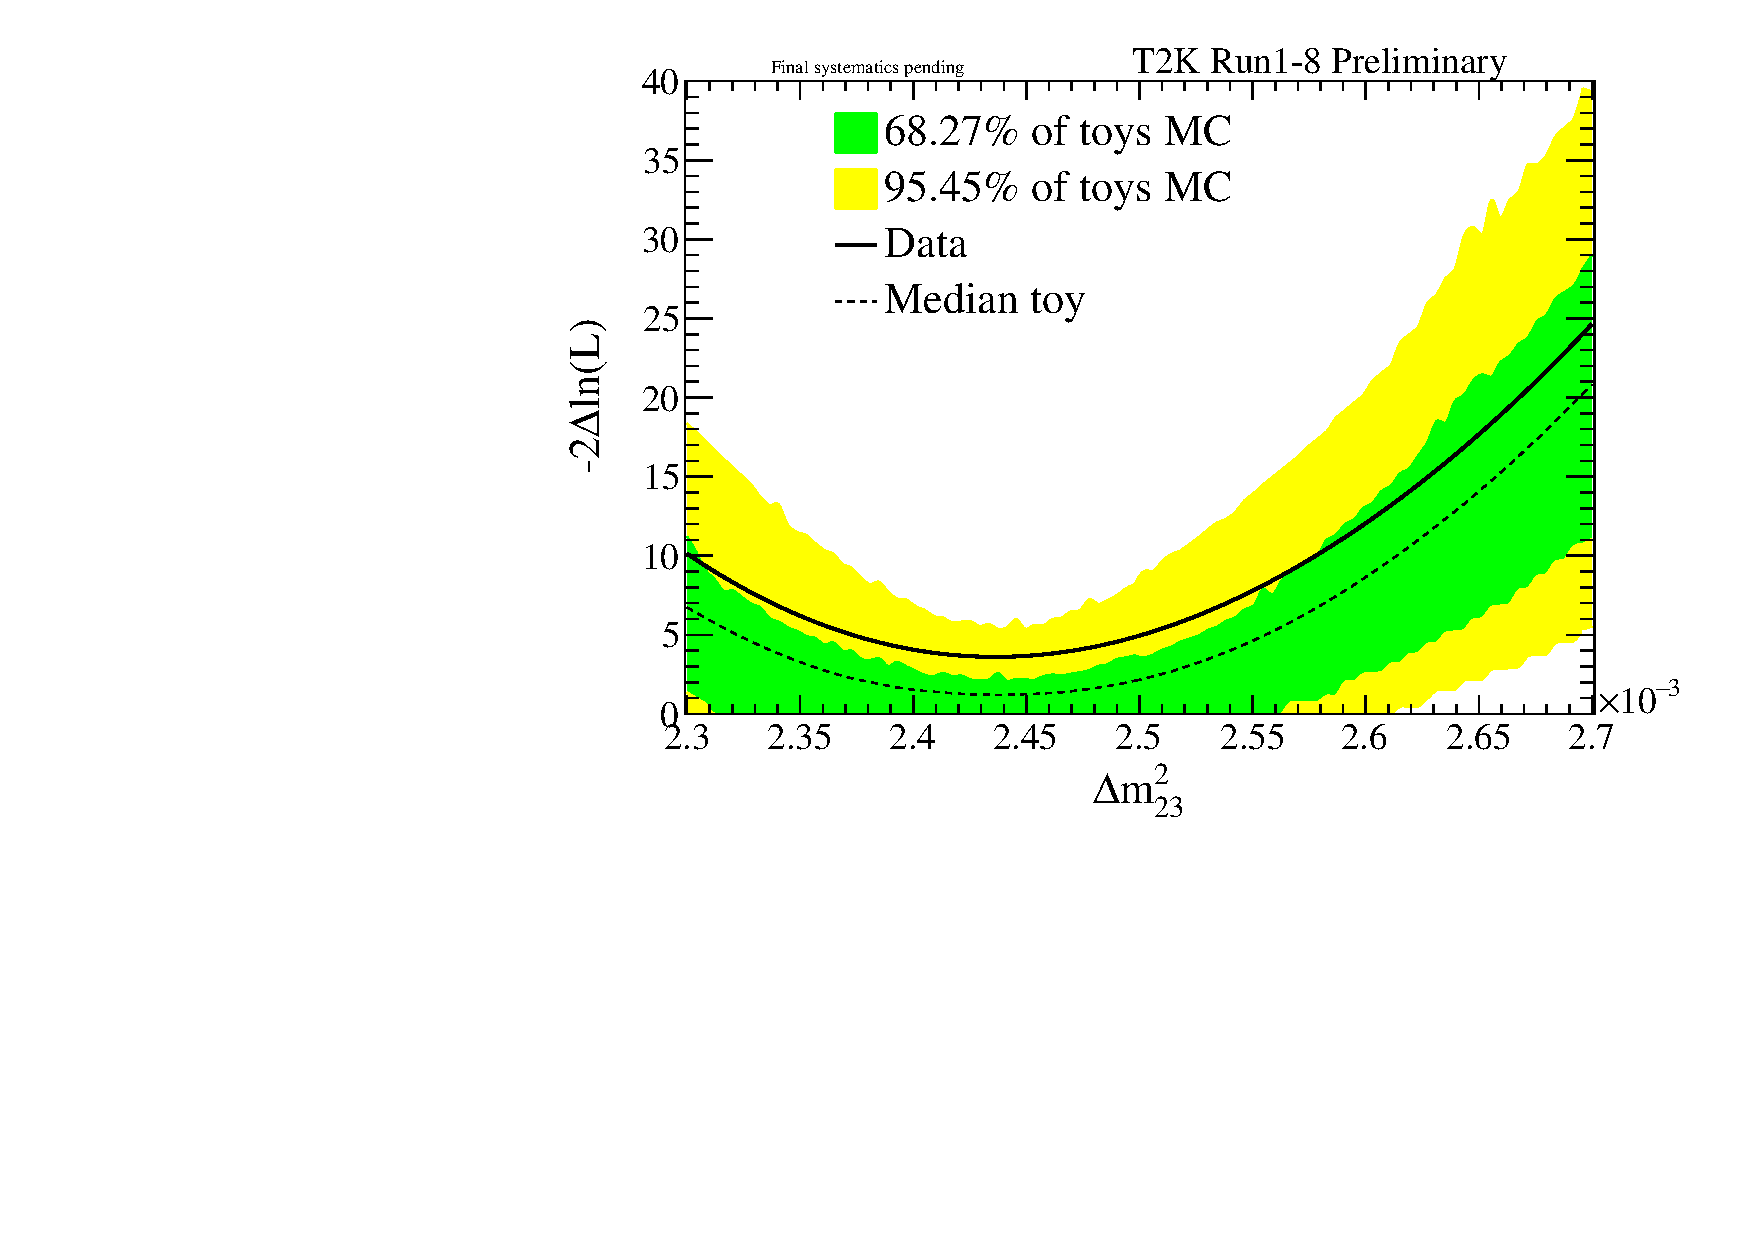
\includegraphics[width=0.9\textwidth]{comparison/dmsq23/dmsq23_run18_all_twosided_braz_ih}
		\caption{Inverted hierarchy}
	\end{subfigure}
	\caption {
		The distribution of $\Delta\chi^2$ vs \dmsqtwothree obtained with \num{1e4} toy experiments generated with $\Delta m^2_{32} = -2.462 \times 10^{-3} \text{eV}^2\text{ c}^{-4}$ and normal hierarchy is shown. The $\Delta\chi^2$ distributions obtained by fixing the mass hierarchy to normal (left) and inverted (right) are shown, along with the $\Delta\chi^2$ values corresponding to 68.27\% and 95.45\% of the toy experiments, the median toy and the data contour.
	}
	\label{fig:brazilian_dmsq23_bestfit}
\end{figure*}

\subsection {Comparison of $e$-like event rates with expectation}
\label{sec:results:bievent}
It is valuable to see how different values of \deltacp, \ssqthtwothree and hierarchy affect the predicted event rates. \Cref{fig:bievent} shows the predicted $\nueb$ event rate vs $\nue$ event rate for best-fit values of oscillation parameters where \deltacp is varied between CP conserving and maximally CP violating values, and \ssqthtwothree is varied around its best-fit, for both hierarchies. Event rates for a given value of \ssqthtwothree and mass hierarchy are linearly interpolated between those computed for 9 evenly-spaced values of \deltacp from $-\pi$ to $+\pi$ to indicate the behaviour produced by varying \deltacp. The observed event rates with $1\sigma$ errors are also shown. \Cref{fig:bievent}(a) shows $e$-like event rates where the FHC sample includes the \nueCConepi sample, while \cref{fig:bievent}(b) shows $e$-like event rates where the FHC sample does not include the \nueCConepi sample.
\begin{figure*}[htb]
	\center
	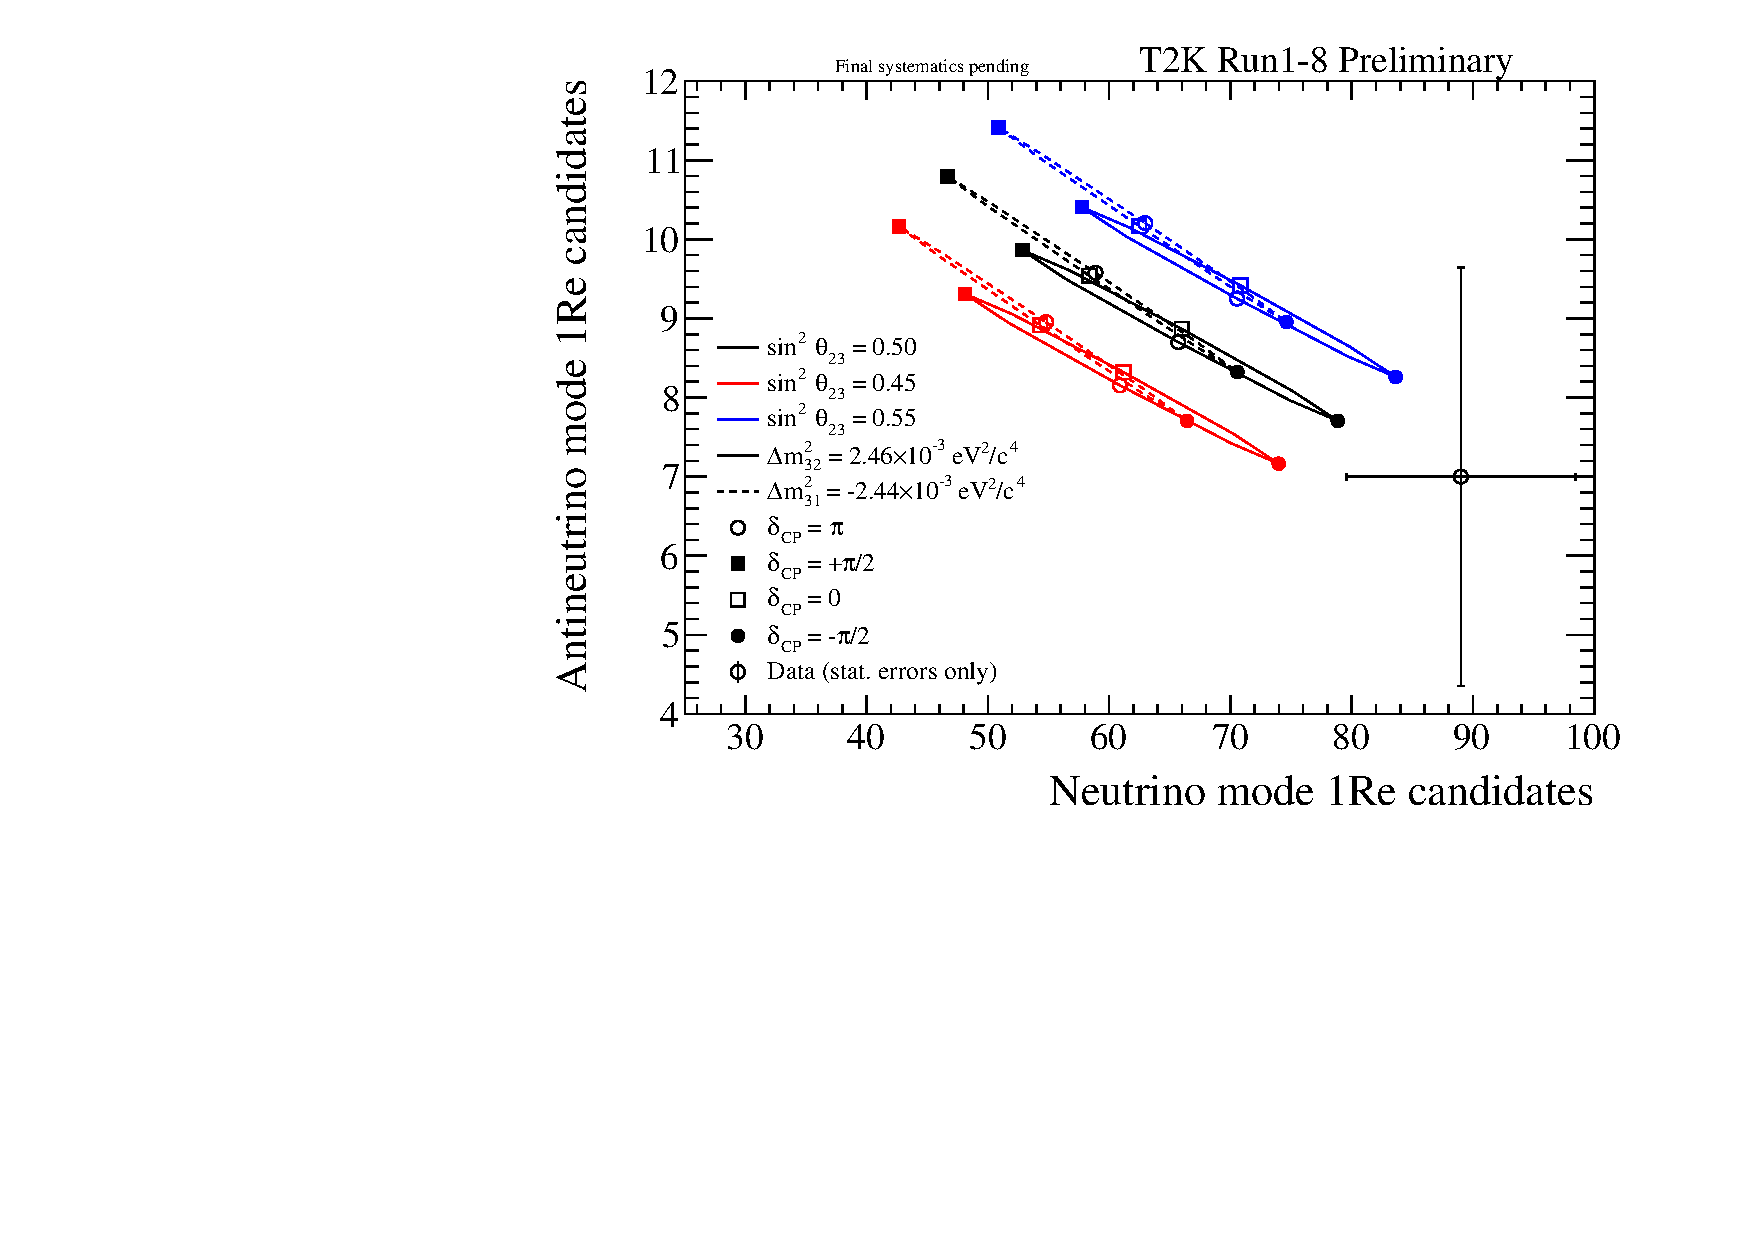
\includegraphics[width=0.7\textwidth]{studies/bievent/ellipse_cc1pi_all}
	\caption {
		This plot shows the candidate RHC one-ring $e$-like event rate vs the candidate FHC one-ring $e$-like event rate for a variety of different oscillation parameter values. Predictions are generated for best-fit values of oscillation parameters for different values of \deltacp, \ssqthtwothree and mass hierarchy. In particular the FHC and RHC event rates are plotted for the CP conserving and maximally CP violating values of \deltacp, with \ssqthtwothree set at the best-fit value and $\pm 1\sigma$ values in both normal and inverted hierarchy. The observed rates with statistical error shown are also included.
	}
	\label{fig:bievent}
\end{figure*}

\clearpage

%%% Local Variables:
%%% mode: latex
%%% TeX-master: "../TN327"
%%% End:
